% Author Thomas C. Hales
% Copyright Thomas C. Hales
% Format latex.
% 

%!TEX TS-program = latex    
%% This line is for TexShop. 

% Revision history. See svn.
% Document created Dec 6, 2002
% Revision started Jan 2007, from published DCG.

\documentclass[cup9a]{cupbook}
%% Cambridge University Press Macros from
%% https://authornet.cambridge.org/information/productionguide/laTex_files/

%
\usepackage{graphicx}
\usepackage{verbatim}
\usepackage{latexsym}
\usepackage{amsfonts}
%\usepackage{amsthm}
\usepackage{amsmath}
%\usepackage{mathidx}
\usepackage{makeidx}
\usepackage{multicol}
\usepackage{crop}
\usepackage{txfonts}
%\usepackage{pdfsync}  %for TexShop sync.
\usepackage[letterpaper,colorlinks=true,
            ps2pdf,hyperindex=true]{hyperref}
%\usepackage{mparhack} %http://www.tex.ac.uk/cgi-bin/texfaq2html?label=marginparside
\usepackage{multind}
\usepackage{url}

% This file contains local settings and system dependencies



% Auxiliary directories
\def\ps{../../../../Pictures/kep07ps}  % flypaper graphics
\def\pdf{/Users/thomashales/Pictures/collect_geom} % tarski graphics

\def\showgraphics{f}  
% t: display graphics (there are none to show yet)
% f (default): print a "no graphics logo" where graphics would normally go.


\def\displayallproof{t} 
% t (default): display all proofs.
% f: print documents without the proofs-- theorem statements only

\def\displayrating{f}
% t (default): display all ratings (verbose is also true)
% f : don't show them.

\def\verbose{f}
% f (default): do not display debugging information,
% t : display debug information and information about the formalization.

\def\tarskipagesep{f}
% f (default): no page breaks between lemmas in tarski collection.
% t :add page breaks

\def\tarskistrip{f}
% f (default): preserves control sequences in tarski collection
% t: control sequences in tarski collection are stripped and printed to an auxiliary file.

\def\tarskidump{f}
% t : dump tarski guid data to external write file.
% f (default) : don't use external write file.
 
%-%
% --Repository--
%-%
% generate revision number by
% svn propset svn:keywords "LastChangedRevision" kepmacros.tex
\def\svninfo{%
  TeXed on \today; \hfill\break
  Repository Root: https://flyspeck.googlecode.com/svn \hfill\break
  SVN $LastChangedRevision$
  }

%-%
% --Fonts--
%-%
\font\twrm=cmr8

%-%
% --Graphics--
%-%
%set \showgraphics option in flag_fly.tex
% flypaper graphics
\def\myincludegraphics#1{%
      \if\showgraphics t{\includegraphics{#1}}%
      \else{
\includegraphics{noimage.eps}}\fi}
\def\szincludegraphics[#1]#2{%
      \if\showgraphics t{\includegraphics{#2}}%
      \else{
\includegraphics{noimage.eps}}\fi}

% kepler graphics
\def\pdffigtemplatex#1#2#3{%
\begin{figure}[htb]%
  \centering
  \myincludegraphics{\pdfp/#1}
  \caption{#3}
  \label{fig:#2}%
\end{figure}%
}
\def\pdfg#1#2#3{\if\showgraphics t{\pdffigtemplatex{#1}{#2}{#3}}\else{}\fi}


% tarski graphics
\def\pdffigtemplate#1#2#3{%
\begin{figure}[htb]%
  \centering
  \myincludegraphics{\pdf/#1}
  \caption{#3}
  \label{tarski:fig:#2}%
\end{figure}%
}
\def\pdffig#1#2#3{\if\showgraphics t{\pdffigtemplate{#1}{#2}{#3}}\else{}\fi}

%-%
% --Footnotes--
%-%
% http://help-csli.stanford.edu/tex/latex-footnotes.shtml
\long\def\symbolfootnote[#1]#2{\begingroup%
\def\thefootnote{\ensuremath{\fnsymbol{footnote}}}\footnote[#1]{#2}\endgroup}

%-%
% --Special Formatting--
%-%
% http://en.wikibooks.org/wiki/LaTeX/Formatting#List_Structures
\renewcommand{\labelitemii}{$\star$}


%-%
% --Indexing, References, Citations--
%-%
\def\indy#1#2{\index{index/#1}{#2}}

%-%
% --Proof Display--
%-%
% set with \displayallproof in flag_fly. If f, then proofs are swallowed.
%% "proved" environment. toggle with \displayallproof
%
\def\hide#1{}
\def\swallowed{\relax}
\def\swallow#1\swallowed{}
\newenvironment{iproved}{}{}
\newenvironment{proved}{\resetproved\begin{iproved}}{\end{iproved}}
\def\hideproof{\renewenvironment{iproved}{%
   \centerline{\it -- Proof Proofed --}
  \renewenvironment{itemize}{}{}
  \renewenvironment{enumerate}{}{}
  \def\item{\relax}
  \catcode13=12
  \swallow
}{}}
\def\showproof{\renewenvironment{iproved}{\begin{proof}}{\end{proof}}}
\def\resetproved{\if\displayallproof t\showproof\else\hideproof\fi}



%-%
% --Debugging Information--
%-%
\def\uf#1{{\par\narrower\it #1}} % unfinished manuscript
%% verbose:
\def\rating#1{\if\displayrating t{{\textsc {[rating={\ensuremath {#1}}].\ }}}\else{}\fi}
\def\oldrating#1{\if\displayrating t{{\textsc {[former rating={\ensuremath {#1}}].\ }}}\else{}\fi}
\def\formal#1{\if\verbose t{{\tt [formal: #1].\ }}\else{}\fi}
\def\formalauthor#1{\if\verbose t{{\tt [formal proof by: #1].\ }}\else{}\fi}
\def\footformal#1{\if\verbose t{\footnote{\formal{#1}}}\else{}\fi}
\def\usage#1{\if\verbose t{\symbolfootnote[1]{#1}}\else{}\fi}
\def\move#1#2{\begin{#1} See \ref{#2}.\end{#1}}
\def\FIXX#1{\if\verbose t{\footnote{\tt [#1]}}\else{}\fi}
\def\page#1#2{#2 {\it [dcgp.#1]}}
% first entry Lemma or Sec of DCG, second entry page.
\def\dcg#1#2{{\if\verbose t{{\tt{[DCG-#1]}}\indy{References}{ZC{#2 #1}@{DCG-#1}|page{#2}}}\else{}\fi}}
\def\tlabel#1{\label{#1}\if\verbose t{{\tt [#1].\ }%
   \indy{References}{#1|itt}}\else{}\fi}
\def\ifverbose#1{\if\verbose t{{#1}}\else{}\fi}




%% Indexing
\def\refXX{0} % for unknown links.
\def\showref#1{\ref{#1}{\tt[#1]}\indy{References}{#1}}
\def\oldlabel#1{\label{x-#1}}

\def\tref#1{\ref{#1}\indy{References}{#1}}
\def\itt#1{{\bf #1}}
\def\guid#1{{\tt[#1].\ }\indy{References}{ZA{#1}@{#1}|itt}}
% textsc
\def\calc#1{{\textsc{calc-#1}}\indy{Interval}{{#1}@{#1}}}
\def\newcalc#1{{\textsc{newcalc-#1}}\indy{Interval}{{#1}@{#1 (new XX)}}}
\def\assembly#1{{\textsc{assembly-#1}}\indy{References}{ZD{#1}@{#1}}}
%\def\conseq#1{{\textsc{conseq-#1}}}

%% 


%% Tarski indexing. Write summary data to external file "\mywrite",
% which is generated in tarski.tex
% Need to extend cs character set.  Use this only within a block.
\def\setcat{
\catcode`\-=11
\catcode`\.=11
\catcode`\:=11
\catcode`\0=11
\catcode`\1=11
\catcode`\2=11
\catcode`\3=11
\catcode`\4=11
\catcode`\5=11
\catcode`\6=11
\catcode`\7=11
\catcode`\8=11
\catcode`\9=11
}
\def\tarfe#1#2{{\foote{{\tt[L.E.G:#1]}~\csname #1-sum\endcsname%
  \expandafter\ifx \csname #1-guid\endcsname \relax [XX-BAD-IDENTIFIER]\else{}\fi
  }
  {\csname #1-guid\endcsname{#2}}}}
\def\tarf#1{\tarfe{#1}{}}
\def\tarfE#1{\tarfe{EE}{-\csname #1\endcsname}}
% control sequences will contain [-.0-9:] \catcode`\-=11, etc.
\newtoks\mysummary
\newtoks\myguid
\newtoks\myname
\def\separator{\if\tarskipagesep t{\clearpage}\else%
  \smallskip\hrule height 0.5pt depth 0pt width 60pt\bigskip\fi}
\def\identity#1{#1}
\def\foote#1#2{\footnote{#1~{\it (#2)}}}
\def\marker#1#2{\par\hangafter1\hangindent=1em\noindent{\bf #1:}\quad #2}
\def\name#1{\marker{Name}{#1}\myname={#1}
  \write\myhtml{  "#1", //name}
}
\def\summary#1{\marker{Summary}#1\mysummary={#1}
  % cleanse control sequences for html
  \if\tarskistrip t{
  \def\sqr{sqrt}
  \def\sqrt{sqrt}
  \def\op{\identity}
  \def\epsilon{epsilon}
  \def\Delta{Delta}
  \def\ups{upsilon}
  \def\beta{beta}
  \def\rho{rho}
  \def\CalE{E}
  \def\chi{chi}
  \def\eta{eta}
  \write\myhtml{  "#1", // summary}
  }
  \else\relax\fi
}
\def\guid#1{\if\tarskidump f{{\tt [#1]}}\else{\marker{ID}#1
   \indy{guid}{#1}
   \immediate\write\mywrite{\global\expandafter\def\csname \the\myname-sum \endcsname{\the\mysummary}}
   \immediate\write\mywrite{\global\expandafter\def\csname \the\myname-guid \endcsname{#1}}
   \immediate\write\myhtml{  "#1" // guid}}%
   \fi
}
\def\tag#1{\marker{Tags}#1
   \immediate\write\myhtml{  "#1", // tag}
}
%\def\rating#1{\marker{Rating}#1
%   \write\myhtml{  <rating>#1</rating>}
%}
\newenvironment{tarski}{%
\write\myhtml{new Tarski(}
%\def\name   {\marker{Name}}
%\def\summary{\marker{Summary}}
%\def\tag    {\marker{Tags}}
\def\rating {\marker{Rating}}
\def\hol{\marker{HOL-Light}}
%\def\guid   {\marker{ID}}
\def\tlabel{\label}
}{\separator\immediate\write\myhtml{),}
}
\newenvironment{tarskidata}{\write\myhtml{var tarskis=[}}
{
\immediate\write\myhtml{];}
}
%% tarski indexing
%\def\tarf#1{\footnote{{\tt geom-#1~\ref{#1}}\indy{ZA{#1}@{#1}}}}




%-%
% --Symbols--
%-%
% norm
\def\|{{\hskip0.1em|\hskip-0.15em|\hskip0.1em}}
\def\mid{\ :\ }
\def\norm#1#2{\|#1 - #2\|}
\def\normo#1{{\|#1\|}}
\def\sland{\ \land\ }
% Sam's
\def\myscorept{\text{ \sl pt}}
\def\qrtet{{quasi-regular tetrahedron}}
\def\qrtets{{quasi-regular tetrahedrons}}
\def\tomcite{{}}
\DeclareMathOperator{\myscore}{\sigma}
 \DeclareMathOperator{\gma}{gma}
 \DeclareMathOperator{\score}{\sigma}
 \DeclareMathOperator{\sol}{sol}
 \DeclareMathOperator{\dih}{dih}
\newtheorem{calcf}{Calculation}[subsection]

% mathcal
\def\CalB{{\mathcal B}}
\def\CalC{{\mathcal C}}
\def\CalD{{\mathcal D}}
\def\CalE{{\mathcal E}}
\def\FF{{\mathcal F}}
\def\CalF{{\mathcal F}}
\def\CalQ{{\mathcal Q}}
%\def\CalW{{\mathcal W}}
\def\CalR{{\mathcal R}}
\def\CalS{{\mathcal S}}
\def\CalV{{\mathcal V}}
\def\T{{\mathcal T}}
\def\Q{{\mathcal Q}}


% brackets
\def\leftopen{]}
\def\leftclosed{[}
\def\rightopen{[}
\def\rightclosed{]}

%% obsolete
\def\leftb{[}
\def\rightb{]}

% squiqqly relations
\def\seq{\approx}
\def\sle{\preceq}
\def\sge{\succeq}
\def\slt{\prec}
\def\sgt{\succ}

% mathbb
\def\R{{\mathbb R}}
\def\N{{\mathbb N}}
\newcommand{\ring}[1]{\mathbb{#1}}
\def\A{{\mathbf A}}
\def\Rp{\ring{R}^{3\,\prime}}

% operatorname
\def\op#1{{\operatorname{#1}}}
\def\optt#1{{\operatorname{{\texttt{#1}}}}}

\def\opat{\op{@}}
\def\atn{\op{arctan\ensuremath{_2}}}
\def\azim{\op{azim}}
\def\sol{\operatorname{sol}}
\def\vol{\op{vol}}
\def\quo{\operatorname{quo}}
\def\anc{\operatorname{anc}}
\def\cro{\operatorname{crown}}
%\def\vor{\operatorname{vor}}
%\def\svor{\operatorname{svor}}
\def\sign{\operatorname{sign}}
\def\octavor{\operatorname{octavor}}
\def\dih{\operatorname{dih}}
\def\Adih{\operatorname{Adih}}
\def\arc{\operatorname{arc}}
\def\cosarc{\operatorname{cosarc}}
\def\rad{\operatorname{rad}}
\def\gap{\operatorname{gap}}
\def\sc{{\operatorname{sc}}}
\def\geom{{\operatorname{g}}}
\def\anal{{\operatorname{an}}}
\def\PM{\operatorname{PM}}
\def\bool{\operatorname{bool}}
\def\true{\op{true}}
\def\false{\op{false}}
\def\flat{\operatorname{flat}}
\def\tangle#1{\langle #1\rangle}
\def\ceil#1{\lceil #1\rceil}
\def\floor#1{\lfloor #1\rfloor}
\def\ups{\upsilonup} % Needs txfonts; else use \upsilon
\def\orgn{\varthetaup} % center of packing
%\def\comp#1{\llbracket #1 \rrbracket}
\def\comp#1{[#1]}
\def\Wdart{W_{\text{dart}}}
\def\Wedge{W_{\text{edge}}}
\def\cell{\operatorname{cell}}

\def\SA{A}
\def\SB{B}
\def\SC{C}
\def\SD{D}
\def\SE{E}
\def\del{\partial}
\def\doct{\delta_{oct}}
\def\dtet{\delta_{tet}}
\def\pt{\hbox{\it pt}}
\def\hm{{h_0}} % 1.26
%\def\Vol{\hbox{vol}}
\def\scoregoal{8\,\pt}
\def\maxpi{\pi_{\max}}
\def\tausc{{\tau\!\operatorname{sc}}}
\def\piF{{\pi_F}}
\def\xiG{\xi_\Gamma}
\def\piG{\pi_\Gamma}
\def\xiV{\xi_V}
\def\xik{\xi_\kappa}
\def\xikG{\xi_{\kappa,\Gamma}}
\def\piV{\pi_V}
\def\tauLP{{\tau_{\hbox{\twrm LP}}}}
\def\DLP{\operatorname{D}_{\hbox{\twrm LP}}}
\def\ZLP{\operatorname{Z}_{\hbox{\twrm LP}}}
\def\tlp{\tau_{\hbox{\twrm LP}}}  % 2 args (p,q) tri, quad
\def\sLP{\sigma_{\hbox{\twrm LP}}}  % 2 args (p,q) tri, quad
\def\squander{(4\pi\zeta-8)\,\pt}
\def\trgt{\operatorname{\it{target}}}
\def\tildeF{{\hbox{$\tilde F$}}}
\def\zloop{{z}_{loop}}
\def\dloop{{\delta}_{loop}}
\def\sqr{\sqrt}
\def\tildeV{V^{\CalS}}
%\def\BigD{\Delta}
%\def\bigd{\Delta^0}
\def\FCinner{\op{FC}_{\text{inner}}}
\def\FC{\op{FC}}
\def\FCR{\op{FCR}}
\def\rogFC{\op{rog}^0_{\text{FC}}}
\def\chino{\chi_0}

\def\x#1{\op{\bf c}{#1}}  % marks context \x(p,r).
\def\xs#1{\op{\bf sc}{#1}}  % marks special context \x(p,r,s).
\def\xtazimlt{\x{(3,1: \op{azim}(\op{gap}) <\pi)}}
\def\xtazimge{\x{(3,1: \op{azim}(\op{gap}) \ge \pi)}}
\def\xfgap{\x{(4,1:\op{gap})}}
\def\y#1{\op{\bf ep}{#1}}  % marks edge parameters \y(n,k).
\def\pqr#1{#1} % marks type (p,q,r).
%\def\pqr#1{\op{\bf typ}{#1}} % marks type (p,q,r).

%% HYPERMAP macros:
% avoid e for both hypermap edge and edge {v,w}
\def\e{\varepsilonup}
\def\ocirc{}



%% FORMULATION macros:
\def\lam{\lambda}
\def\Lam{\Lambda}
\def\bl{{\underline{\lam}}}
\def\bm{{\underline{\mu}}}
\def\angle#1#2#3{{\op{angle}(#1,{#2,#3})}}


\def\card{\op{card}}

% accent used in India citation in Overview.
\def\=#1{\accent"16 #1}
\def\i{I}
%\def\={\relax}



%% Enclosed CALE control sequences:
\expandafter\def\csname 2t0-doesnt-pass-through\endcsname{01}
\expandafter\def\csname E1453\endcsname{02}   
\expandafter\def\csname dcg-p89\endcsname{03}   
\expandafter\def\csname enclosed-v\endcsname{04}   
\expandafter\def\csname 277\endcsname{05}   
\expandafter\def\csname 245\endcsname{06}   
\expandafter\def\csname 245bis\endcsname{07}   
\expandafter\def\csname node\endcsname{08}   
\expandafter\def\csname E:part4:1\endcsname{09}   
\expandafter\def\csname E:part4:2\endcsname{10}   
\expandafter\def\csname E:part4:3\endcsname{11}   
\expandafter\def\csname E:part4:4\endcsname{12}   
\expandafter\def\csname E:part4:5\endcsname{13}   
\expandafter\def\csname E:part4:6\endcsname{14}   
\expandafter\def\csname E:part4:7\endcsname{15}   
\expandafter\def\csname E:part4:8\endcsname{16}   
\expandafter\def\csname E:part4:9\endcsname{17}   
\expandafter\def\csname E:part4:10\endcsname{18}   
\expandafter\def\csname dcg-p142\endcsname{19}   
\expandafter\def\csname convex-quad\endcsname{20}   
\expandafter\def\csname last:E\endcsname{21}
\expandafter\def\csname rem2.7\endcsname{22}     
\expandafter\def\csname pass-anchor\endcsname{23}

%% 
 
 
 
 
 
 
 


 \crop
%\makeindex

% CUP BOOK CLASS SPECIFIC
\newtheorem{lemma}{Lemma}[chapter]
\newtheorem{definition}{Definition}[chapter]
\newtheorem{remark}{Remark}[chapter]
\newtheorem{theorem}{Theorem}[chapter]
\newtheorem{corollary}{Corollary}[chapter]
\newtheorem{example}{Example}[chapter]
\newtheorem{claim}{Claim}[chapter]
\newtheorem{notation}{Notation}[chapter]
\newtheorem{assumption}{Assumption}[chapter]
\newtheorem{interpretation}{Interpretation}[chapter]
\newtheorem{conjecture}{Conjecture}[chapter]
\newtheorem{note}{Author's Note}[chapter]
%%%%%%%%%%%%%%%%%%%%%%%%%%%%%%%%%%%%%%%%%%%%%%%%%%%%

\begin{document}
\raggedbottom  % for now.
%\raggedright  % don't worry for now.

    \title{Flyspeck :
      %\\ \phantom{Hello}
      \\  A Blueprint for the Formal Proof of the Kepler Conjecture
      \\ (2009 Version)}
      
      %\\{XX Sphere Packings From the Ground Up}
    \author{Thomas C. Hales}
    \maketitle
    \frontmatter
    \tableofcontents
    \thanks

\mainmatter

\noindent

\bigskip\noindent
This material is based upon work supported by the National Science
Foundation under
Grants 0503447 and 0804189.

\bigskip\noindent\svninfo 

%\bigskip\noindent
%A pdf of an earlier version of this work appears at\hfill\break 
%\url{http://www.math.pitt.edu/~thales/papers/Flyspeck_Blueprint_2008.pdf}.

\bigskip\noindent
%% XX Thanks to Tran Nam Trung on the hypermap chapter.

%% INDEX OF FORMAL TERMS.

\def\idx#1#2{\indy{Spec}{{\tt #1}; #2}}
\def\idz#1#2#3{\indy{Spec}{{\tt #1}; #2; {\tt \textbackslash \string#3}}}
\idx{pt}{$\pt$}
\idz{atn2~x~~y}{$\atn(x,y)$}{atn}
\idx{sqrt8}{$\sqrt8$}
\idx{sqrt2}{$\sqrt2$}
\idx{t0}{$t_0$}
\idx{two\_t0}{$2t_0$}
\idx{square\_2t0}{$(2t_0)^2$}
\idx{square\_4t0}{$(4t_0)^2$}
\idx{zeta}{$\zeta$}
\idz{doct}{$\doct$}{doct}
\idz{dtet}{$\dtet$}{dtet}
\idx{pi\_rt18}{$\pi/\sqrt{18}$}
\idx{rogers}{$\sqrt2/\zeta$}
\idx{compression\_cut}{$1.41$}
\idz{squander\_target}{$\squander$}{squander}
\idz{xi\_gamma}{$\xiG$}{xiG}
\idz{xiV}{$\xiV$}{xiV}
\idx{xi'\_gamma}{$\xiG'$}
\idz{xi\_kappa}{$\xik$}{xik}
\idz{xi\_kappa\_gamma}{$\xikG$}{xikG}
\idz{pi\_max}{$\maxpi$}{maxpi}
\idx{t4}{$t_4$}
\idx{t5}{$t_5$}
\idx{t6}{$t_6$}
\idx{t7}{$t_7$}
\idx{t8}{$t_8$}
\idx{t9}{$t_9$}
\idx{t10}{$t_{10}$}
\idx{s5}{$s_5$}
\idx{s6}{$s_6$}
\idx{s7}{$s_7$}
\idx{s8}{$s_8$}
\idx{s9}{$s_9$}
\idx{s10}{$s_{10}$}
\idx{eps0}{$\epsilon_0$}
\idx{Z31}{$Z_{3,1}$}
\idx{D31}{$D_{3,1}$}
\idx{Z31}{$Z(\y{(3,1)})$}
\idx{Z32}{$Z(\y{(3,2)})$}
\idx{Z33}{$Z(\y{(3,3)})$}
\idx{Z41}{$Z(\y{(4,1)})$}
\idx{Z42}{$Z(\y{(4,2)})$}
\idx{D31}{$D(\y{(3,1)})$}
\idx{D32}{$D(\y{(3,2)})$}
\idx{D33}{$D(\y{(3,3)})$}
\idx{D41}{$D(\y{(4,1)})$}
\idx{D42}{$D(\y{(4,2)})$}
\idx{D51}{$D(\y{(5,1)})$}
\idz{delta\_x x1 ... }{$\Delta(x_1,\ldots)$}{Delta}
\idx{delta\_x4 x1 ... }{$\Delta_4(x_1,\ldots)$}
\idx{delta\_x6 x1 ... }{$\Delta_6(x_1,\ldots)$}
\idz{ups\_x x1 ...}{$\ups(x_1,\ldots)$}{ups}
\idz{eta\_x x1 x2 x3}{$\eta(\sqrt{x_1},\sqrt{x_2},\sqrt{x_3})$}{eta}
\idz{eta\_y y1 y2 y3}{$\eta(y_1,y_2,y_3)$}{eta}
\idz{rho\_x x1 ... }{$\rho(x_1,\ldots)$}{rho}
\idx{rad2\_y y1 ... }{$(\rad_V\{v_0,v_1,v_2,v_3\})^2,\ y_1 = |v_0-v_1|,\ldots$}
\idz{chi\_x x1 ... }{$\chi(x_1\ldots)$}{chi}
\idz{dih\_x x1 ... }{$\dih(\sqrt{x_1},\ldots)$}{dih}
\idz{dih\_y y1 ... }{$\dih(y_1,\ldots)$}{dih}
\idx{dih2\_x x1 x2 ... }{$\dih(\sqrt{x_2},\ldots)$}
\idx{dih2\_y x1 x2 ... }{$\dih(y_2,\ldots)$}
\idx{dih3\_x x1 x2 ... }{$\dih(\sqrt{x_3},\ldots)$}
\idx{dih3\_y x1 x2 ... }{$\dih(y_3,\ldots)$}
\idz{sol\_x x1 ... }{$\sol(v_0,\ldots),\ x_1=|v_0-v_1|^2,\ldots$}{sol}
\idz{sol\_y y1 ... }{$\sol(v_0,\ldots),\ y_1=|v_0-v_1|,\ldots$}{sol}
\idx{vol\_x x1 ... }{$\sqrt{\Delta(x_1,\ldots)}/12$}
\idz{beta psi theta}{$\beta_\psi\theta$}{beta}
\idz{arclength a b c}{$\arc(a,b,c)$}{arc}
\idx{volR a b c}{$\op{volR}(a,b,c)$}
\idx{solR a b c}{$\op{solR}(a,b,c)$}
\idx{dihR a b c}{$\op{dihR}(a,b,c)$}
\idx{vorR a b c}{$\op{sovoR}(a,b,c,\lambda_{oct})$}
\idx{denR a b c}{$\delta(a,b,c)$}
\idx{tauR a b c}{$\op{sovoR}(a,b,c,\lambda_{sq})$}
\idx{qy y1 y2 y3 t}{$\op{quovol}(a,b,c)$}
\idx{quo\_x x y z}{}
\idx{qn y1 y2 z t}{}
\idx{phi h t}{}
\idx{phi0}{}
\idx{eta0 h}{}
\idx{crown h}{}
\idx{anc y1 y2 y6}{}
\idx{K0 y1 y2 y6}{}
\idx{AH h t}{}
\idx{BHY y}{}
\idx{KY y1 y2 y3 y4 y5 y6}{}
\idx{KX x1 x2 x3 x4 x5 x6}{}
\idx{vor\_analytic\_x x1 x2 x3 x4 x5 x6}{}
\idx{vor\_analytic\_x\_flipped x1 x2 x3 x4 x5 x6}{}
\idx{octavor\_analytic\_x x1 x2 x3 x4 x5 x6}{}
\idx{tau\_analytic\_x x1 x2 x3 x4 x5 x6}{}
\idx{kappa y1 y2 y3 y4 y5 y6}{}
\idx{kappa\_dih\_y y1 y2 y3 y5 y6 d}{}
\idx{level\_at h t}{}
\idx{vorstar h1 h2 h3 a1 a2 a3 t}{}
\idx{vort\_y y1 y2 y3 y4 y5 y6 t}{}
\idx{vor\_0\_y y1 y2 y3 y4 y5 y6}{}
\idx{tau\_0\_y y1 y2 y3 y4 y5 y6}{}
\idx{vor\_0\_x x1 x2 x3 x4 x5 x6}{}
\idx{tau\_0\_x x1 x2 x3 x4 x5 x6}{}
\idx{vort\_x x1 x2 x3 x4 x5 x6 t}{}
\idx{tauVt\_x x1 x2 x3 x4 x5 x6 t}{}
\idx{vorA\_x x1 x2 x3 x4 x5 x6}{}
\idx{tauA\_x x1 x2 x3 x4 x5 x6}{}
\idx{vorC0\_x x1 x2 x3 x4 x5 x6}{}
\idx{tauC0\_x x1 x2 x3 x4 x5 x6}{}
\idx{vorC\_x x1 x2 x3 x4 x5 x6}{}
\idx{tauC\_x x1 x2 x3 x4 x5 x6}{}
\idx{v0x x1 x2 x3 x4 x5 x6}{}
\idx{v1x x1 x2 x3 x4 x5 x6}{}
\idx{gamma\_x x1 x2 x3 x4 x5 x6}{}
\idx{tau\_gamma\_x x1 x2 x3 x4 x5 x6}{}
\idx{rad2\_x x1 x2 x3 x4 x5 x6}{}
\idx{sigma\_qrtet\_x x1 x2 x3 x4 x5 x6}{}
\idx{sigma1\_qrtet\_x x1 x2 x3 x4 x5 x6}{}
\idx{tau\_sigma\_x x1 x2 x3 x4 x5 x6}{}
\idx{sigma32\_qrtet\_x x1 x2 x3 x4 x5 x6}{}
\idx{mu\_flat\_x x1 x2 x3 x4 x5 x6}{}
\idx{taumu\_flat\_x x1 x2 x3 x4 x5 x6}{}
\idx{mu\_upright\_x x1 x2 x3 x4 x5 x6}{}
\idx{mu\_flipped\_x x1 x2 x3 x4 x5 x6}{}
\idx{vor\_0\_x\_flipped x1 x2 x3 x4 x5 x6}{}
\idx{octavor0\_x x1 x2 x3 x4 x5 x6}{}
\idx{nu\_x x1 x2 x3 x4 x5 x6}{}
\idx{nu\_gamma\_x x1 x2 x3 x4 x5 x6}{}
\idx{taunu\_x x1 x2 x3 x4 x5 x6}{}
\idx{octa\_x x1 x2 x3 x4 x5 x6}{}
\idx{sigmahat\_x x1 x2 x3 x4 x5 x6}{}
\idx{sigmahat\_x' x1 x2 x3 x4 x5 x6}{}
\idx{sigmahatpi\_x x1 x2 x3 x4 x5 x6}{}
\idx{tauhat\_x x1 x2 x3 x4 x5 x6}{}
\idx{tauhatpi\_x x1 x2 x3 x4 x5 x6}{}
\idx{pi\_prime\_tau k0 k1 k2}{}
\idx{pi\_prime\_sigma k0 k1 k2}{}



  % Formal Spec Index.

\smallskip
\newpage




%%%%%%%%%%%%%%%%%%%%%%%%%%%%%%%%%%%%%%%%%%%%%%%%%%%%
   \newpage
   %\setcounter{chapter}{-1}
   %\chapter{Preface}

%%%%%%%%%%%%%%%%%%%%%%%%%%%%%%%%%%%%%%%%%%%%%%%%%%%%
  
    



In this \chap, trigonometry is developed analytically.  The basic
trigonometric functions are defined by their power series
representations, and calculus of a single real variable is used to
develop the basic properties of these functions.  We give a brief
review of the definitions and properties.


\subsection{sine and cosine}

The cosine and sine functions are defined by their infinite series:
    \begin{equation}\label{eqn:cos-def}\cos(x) = 1 - x^2/2! + x^4/4! \cdots,\qquad
  \sin(x) = x - x^3/3! + x^5/5! \cdots.
    \end{equation}
Convergence is absolute for every real number $x$.
The series can be evaluated at $0$:
    \begin{equation}\label{eqn:cos0}
    \cos(0) = 1,\qquad \sin(0) = 0.
    \end{equation}

The series may be differentiated term-by-term to establish the identities:
    \begin{equation}\label{eqn:cos'}
    \frac{d \cos(x)}{dx} = -\sin(x),\qquad \frac{ \sin(x)}{dx} = \cos(x).
    \end{equation}

The powers $(\cos(x))^n$ and $(\sin(x))^n$ are conventionally written
$\cos^n(x)$ and $\sin^n(x)$.

Trigonometric identities follow easily from these definitions.  We
give a couple of examples.

\begin{lemma}\label{lemma:circle}
   $$\cos^2(x) + \sin^2(x) = 1.$$
\end{lemma}

\begin{proof}
By basic properties of derivatives and Equation~\ref{eqn:cos'},
the derivative of the function $f(x) = \cos^2(x) +\sin^2(x)$ is
identically zero.   So the function is constant.  From
Equation~\ref{eqn:cos0}, it follows that $f(x)=f(0)=1$.
\end{proof}

\begin{lemma}\label{lemma:sin_add}
  $$\begin{array}{lll}
  \sin(x+y) &= \sin(x)\cos(y) + \cos(x)\sin(y)\\
  \cos(x+y)  &= \cos(x)\cos(y) - \sin(x)\sin(y).
  \end{array}$$
\end{lemma}

\begin{proof}
Fix $y$.  Let
    $$\begin{array}{lll}
    f(x) = &(\cos(x+y) - \cos(x)\cos(y) +
    \sin(x)\sin(y))^2 +\\ & (\sin(x+y) -\sin(x)\cos(y) -
    \cos(x)\sin(y))^2.
    \end{array}$$
The derivative of $f$ is identically zero.  The function is
therefore constant. Also, $f(0)=0$.  Thus, $f$ is identically zero.
If a sum of real squares is zero, the individual terms are zero. The
identities follow.
\end{proof}

\begin{lemma}\label{lemma:cos_even}
The cosine is an even function.  The sine is an odd
function.
    $$\cos(-x) = \cos(x),\quad\sin(-x) = -\sin(x).$$
\end{lemma}

\begin{proof}
The derivative of
    $$(\cos(-x) - \cos(x))^2 + (\sin(-x) +\sin(x))^2$$
is identically zero.  Argue as in the previous lemmas.
\end{proof}

\subsection{$\pi$}
\label{sec:pi}

It is known that the cosine function has a unique root between $0$
and $2$. The constant $\pi$ is defined as twice that root.  Thus, by
definition $\cos(\pi/2) = 0$, and the cosine has no root greater
than $0$ and less than $\pi/2$. The $\cos$ function is in fact
positive on the interval $\leftclosed 0,\pi/2\rightopen$.


\begin{lemma}\label{lemma:sin_pi2}
    $\sin (\pi/2) = 1.$
\end{lemma}

\begin{proof}
The derivative of $\sin$ is non-negative between $0$ and $\pi/2$.
Its value at $0$ is $0$.  Thus, $\sin$ is non-negative on
$[0,\pi/2]$.  We can check the identity of the lemma by checking
that the squares of the two sides are equal. Then $\sin^2(\pi/2) =
{1-\cos^2(\pi/2)} = 1$.
\end{proof}

\begin{lemma}\label{lemma:sin_cos}
    $$\sin(\pi/2 - x) = \cos(x).$$
\end{lemma}

\begin{proof}
    Apply the addition law for the sine function,
    $$\sin(\pi/2 - x) = \sin(\pi/2)\cos(-x) + \cos(\pi/2)\sin(-x)$$
    and use
    $\sin(\pi/2) = 1$, $\cos(\pi/2) = 0$.  Then use that $\cos$ is
    an even function.
\end{proof}

Similarly, $\cos(\pi/2 - x) = \sin(x)$ or $\cos(\pi/2 + x) =
-\sin(x)$, $\sin(\pi/2 + x) = \cos(x)$.  Further,
    $$\begin{array}{lll}
      \sin(\pi + x) &= \phantom{-}\cos(\pi/2 + x) &= -\sin(x),\\
      \cos(\pi + x) &= -\sin(\pi/2 + x) &= -\cos(x),\\
      \sin(2\pi + x) &= -\sin(\pi + x) &= \phantom{-}\sin(x),\\
      \cos(2\pi + x) &= -\cos(\pi + x) &= \phantom{-}\cos(x).
      \end{array}$$


\subsection{tangent}
\label{sec:tangent}

\begin{definition}\label{def:tan}
Let $\tan(x) = \sin(x)/\cos(x)$, defined when $\cos(x)\ne0$.
\end{definition}


\begin{lemma}\label{lemma:tan_add}
    If $\cos(x)\ne 0$, $\cos(y)\ne 0$, and $\cos(x+y)\ne0$ then
    $$\tan(x+y) = \frac{\tan(x) + \tan(y) }{ 1 - \tan(x)\tan(y)}$$
\end{lemma}

\begin{proof}
  Divide the first line of Lemma~\ref{lemma:sin_add} by the second
  line of the same lemma.
\end{proof}

\begin{lemma}\label{lemma:tan_pi4}
    $$\tan(\pi/4) = 1.$$
\end{lemma}

\begin{proof}
    $$\tan(\pi/4) = \sin(\pi/2-\pi/4)/\cos(\pi/4) =
    \cos(\pi/4)/\cos(\pi/4) = 1.$$
\end{proof}


\subsection{arctangent}

We review the properties of the arctangent function.

\begin{definition}\label{definition:arctan}
There is a unique function $\arctan:\ring{R}\to\ring{R}$ with
image $(-\pi/2,\pi/2)$ such that
    $$\tan(\arctan x) =x.$$
\end{definition}

If $-\pi/2 < x < \pi/2$, then also $\arctan(\tan(x)) = x$. In
particular,
    $$\arctan(1) = \arctan(\tan(\pi/4)) = \pi/4.$$


The function $\arctan$ is differentiable with derivative
    $$\frac{d \arctan(x)}{dx} = \frac{1}{1 + x^2}.$$
The derivative is everywhere positive, and the function $\arctan$ is
strictly increasing.


\subsection{other inverse trig functions}

Other inverse trigonometric functions will generally be reduced to
the arctangent.

\begin{definition}\label{definition:arccos}
$\arccos y$ is the function on the interval $[-1,1]$
taking values in $[0,\pi]$ that is the inverse function of $\cos$:
    $$\begin{array}{lll}
        y\in [-1,1] &\Rightarrow \cos(\arccos y) = y\\
        x\in[0,\pi] &\Rightarrow \arccos(\cos x) = x
    \end{array}$$
\end{definition}

\begin{lemma}\label{lemma:sin_arccos} If $y\in[-1,1]$, then
    $$\sin(\arccos(y)) = \sqrt{1-y^2}.$$
\end{lemma}

\begin{proof}
    The range of $\arccos(y)$ is $[0,\pi]$.  On this interval, $\sin$
    is nonnegative.  Thus, we can check the identity by squaring
    both sides.  It then follows from the circle identity
    (Lemma~\ref{lemma:circle}).
\end{proof}


Our preference is to remove the $\arccos$ function whenever
possible, by replacing it with the $\arctan$ function through the
following identity.  We will occasionally be forced to revert to
$\arccos$ when we are near the endpoints $-1$ and $1$ of its domain.

\begin{lemma}\label{lemma:arccos_arctan}  If $y\in (-1,1)$, then
    $$\arccos(y) = \pi/2 - \arctan(\frac{y}{ \sqrt{1-y^2}}).$$
\end{lemma}

\begin{proof} If $y\in (-1,1)$,  $x = \arccos(y)$, 
$z = \arctan(y/\sqrt{1-y^2})$, then
    $-\pi/2 < \pi/2 - x < \pi/2$, and $-\pi/2 < z < \pi/2$.  It is
    therefore enough to check that
        $\tan(\pi/2 - x) = \tan(z)$.
    But
        $$\tan(\pi/2-x) = \frac{\cos(x)}{\sin(x)} = \frac{y}{
        \sin(\arccos(y))} = \frac{y}{ \sqrt{1-y^2}} = \tan(z).$$
\end{proof}

\begin{definition}\label{def:arcsin}
$\arcsin y$ is the function on the interval $\leftclosed
-1,1\rightclosed$ taking values in $[-\pi/2,\pi/2]$ that is the
inverse function of $\sin$:
    $$\begin{array}{lll}
        y\in [-1,1] &\Rightarrow \sin(\arcsin y) = y\\
        x\in[-\pi/2,\pi/2] &\Rightarrow \arcsin(\sin x) = x
    \end{array}$$
\end{definition}

As we do not have need for the arcsine function, we do not develop
any of its properties.





\section{Triangle Inequality}

The set $\ring{R}^n$ is defined as the set of functions
$f:\ring{N}\to\ring{R}$ such that $f(i) = 0$ when $n\le i$. Defined
this way, there are natural inclusions
    $$\ring{R}^0 \subset \ring{R}^1 \subset \ring{R}^2 \cdots$$

We let $\ring{R}^\infty$ be the union of all $\ring{R}^n$.  It is
the set of function $f:\ring{N}\to\ring{R}$ that have finite
support.  We write $v_i$ for the value of the function $v$ at $i$.
We call elements of $\ring{R}^\infty$ {\it vectors}.  There is a
zero vector $0$, defined as the function that is identically zero.

There is an addition and scalar multiplication on $\ring{R}^\infty$
defined by addition and multiplication of functions.
    $$\begin{array}{lll}
    (u + v)_i &= u_i + v_i.\\
    (s u)_i & s u_i,\quad s\in\ring{R}.\\
    \end{array}
    $$
The addition is commutative and associative, and gives
$\ring{R}^\infty$ the usual properties of a vector space. If $u$ and
$v$ both lie in some $\ring{R}^n$, then so do $u+v$ and $s u$.

We define the difference of two vectors as $u - v = u + (-1) v$.

%\begin{definition}
%A set of vectors $V$ is collinear, if there is vector $u$ such that
%for every $v,v'\in V$ there exists $t$ such that $v - v' = t u$.
%\end{definition}

There is a dot product
$$(\cdot):\ring{R}^\infty\to\ring{R}^\infty\to\ring{R}$$ defined by
    $$u\cdot v = \sum_{i=0}^\infty u_i v_i.$$
Only finitely many terms in the sum are nonzero, so it is actually a
finite sum.  The dot product satisfies the following
properties:
    $$\begin{array}{lll}
        u \cdot (v + w) &= u \cdot v + u \cdot w\\
        (u + v)\cdot w &= u \cdot w + v \cdot w\\
        (s u)\cdot w &= s(u \cdot w) = u \cdot (s w)\\
        0 &\le u\cdot u\\
    \end{array}$$


There is a norm
$$|u| = \sqrt{u\cdot u}.$$
It satisfies $| s u | = |s| \, |u|$.  We have $|u|=0$  if and
only if $u=0$, the zero function.

\begin{lemma}[Cauchy-Schwartz inequality]
    $$|u \cdot v| \le |u|\,|v|.$$
Equality holds exactly when $|v|u = \pm |u|v$.  Furthermore,
$u\cdot v = |u|\,|v|$ holds exactly when $|v| u = |u| v$.
\end{lemma}

\begin{proof}
   Let $w = |v| u \pm |u| v$.  Then expanding $w\cdot w$ we get
    $$0\le w\cdot w = 2|u|^2|v|^2 \pm 2|u|\, |v| (u\cdot v) =
    2|u|\,
    |v| (|u|\, |v| \pm (u \cdot v)).$$
    If $2|u| \,|v| = 0$, then $u$ or $v$ is zero, and the result
    easily follows.  Otherwise divide both sides of the inequality
    by the positive quantity $2 |u| \,|v|$ to get the result.
\end{proof}

\begin{lemma}[triangle inequality]
  $$
  |u + v| \le |u| + |v |.
  $$
Equality holds exactly when $|v|u = |u|v$.
\end{lemma}

\begin{proof}
Both sides are nonnegative; it is enough to compare the squares of
both sides.  By the Cauchy-Schwartz inequality,
    $$|u + v|^2 = u\cdot u + 2 u\cdot v + v\cdot v \le
      u\cdot u + 2 | u|\,|v| + v\cdot v = (|u|+|v|)^2.
    $$
The case of equality follows from the case of equality in the
Cauchy-Schwartz inequality.
\end{proof}

There is a distance function $d(u,v) = | u - v|$ that makes
$\ring{R}^\infty$ into a metric space.  The subsets $\ring{R}^n$ are
metric subspaces.






\subsection{coordinates}

Let $\{v_1,v_2,v_3,v_4\}$ be a set of vectors of cardinality four.
There are $6$ (four choose two) different pairs of vectors. We let
$y_{ij} = |v_i-v_j|$ and $x_{ij}=y_{ij}^2$.


%% WW repeated DEF.
\begin{definition}\label{def:delta}  Let 
$$
\begin{array}{lll}
\Delta(x_1,\ldots,x_6) &= x_1 x_4 (- x_1+x_2+x_3- x_4+x_5+x_6)+\\&
            x_2 x_5 (x_1- x_2+x_3+x_4- x_5+x_6)
            +x_3 x_6 (x_1+x_2- x_3+x_4+x_5- x_6)
            - \\&x_2 x_3 x_4- x_1 x_3 x_5- x_1 x_2 x_6- x_4 x_5 x_6
\end{array}
$$
\end{definition}

We write $\Delta_j$ for the $j$th partial derivative of $\Delta$. 
Let $D = \det(v_1-v_0,v_2-v_0,v_3-v_0)$.
Lemma~\ref{tarski:cm4} asserts that 
  $$
  4 D^2 = \Delta(x_{12},x_{13},x_{14},x_{34},x_{24},x_{23}).
  $$
In particular, the polynomial $\Delta$ is positive on values $x_{ij}$
that come from a simplex of positive volume.





\subsection{affine geometry}

%% WW This section is repeated verbatim in tarski.tex

\begin{definition}\label{def:aff} 
 If $S = \{v_1,v_2,\ldots,v_k\}$ 
and $S'=\{v_{k+1},\ldots,v_n\}$ are  finite sets, then
set
	$$\begin{array}{lll}
      \op{aff}\, S &= \{t_1 v_1 +\cdots t_k v_k \mid
	t_1 +\cdots+t_k = 1\}.\\
        \op{aff}_{\pm} (S,S') &= \{t_1 v_1 +\cdots t_n v_n \mid
	t_1 +\cdots+t_n = 1, \pm t_j \ge 0, \text{ for } j>k.\}.\\
        \op{aff}^0_{\pm} (S,S') &= \{t_1 v_1 +\cdots t_n v_n \mid
	t_1 +\cdots+t_n = 1, \pm t_j > 0, \text{ for } j>k.\}.\\
		\end{array}
        $$
\end{definition}

\begin{definition}  If $S = \{v_1,v_2,\ldots,v_n\}$ is a finite set
of points in $\ring{R}^3$, then
set
	$$
        \begin{array}{lll}
          \op{conv}\, S &= \op{aff}_+\, (\emptyset,S)\\
	   \op{conv}^0 S &= \op{aff}^0_+\, (\emptyset,S).\\
           \end{array}
        $$
\end{definition}


\begin{definition}
Let $S=\{v_1,\ldots,v_n\}$ be a finite set of points in 
$\ring{R}^3$.  Let $v\in\ring{R}^3$. Set
  $$\begin{array}{lll}
  \op{cone}(v,S) &= \op{aff}_+(\{v\},S)\\
  \op{cone}^0(v,S) &= \op{aff}^0_+(\{v\},S)\\
  \end{array}
  $$
\end{definition}

\begin{definition} 
Let $S$ be a finite set of points in 
$\ring{R}^3$.  Let $v\in\ring{R}^3$. Set
  $$
  \Omega(v,S) = \{x \mid |v-x| < |w-x|, \forall w\in S\setminus\{v\}\}
  $$
\end{definition}
	
\begin{definition}	
Any set of the form $\op{aff}\{v,w\}$ for some $v\ne w$ is called a 
 {\it line.}
\end{definition}

\begin{definition}  A set $S$ is collinear if there exists
a line that contains every point of $S$.
\end{definition}

\begin{definition}	
If $A=\op{aff}\{u,v,w\}$ for some set $\{u,v,w\}$ that is not collinear,
then $A$ is a {\it plane.}  Sets $\op{aff}(\{u,v\},\{w\})$, with
$\{u,v,w\}$ not collinear, are called half-planes.
\end{definition}

\begin{definition} A set $S$ is  coplanar if there exists
a plane that contains every point of $S$.
\end{definition}

\begin{definition} A set $\op{aff}_{\pm}(\{u,v,w\},\{v'\})$,
with $\{u,v,w,v'\}$ not coplanar, is called a half-space.  If
we replace $\op{aff}_{\pm}$ with $\op{aff}_{\pm}^0$ we have an
{\it open half-space}.
\end{definition}

\section{Angle}



If $u,v$ are given with $u$ and $v$ nonzero, then by the
Cauchy-Schwartz inequality,
    $$-1 \le \frac{u\cdot v}{|u|\,|v|} \le 1.$$

\begin{definition}\label{def:angle}
There is a unique $\theta$ with $0\le\theta\le\pi$ such that
    $$\cos\theta = \frac{u\cdot v}{|u|\,|v|}.$$
It is the {\it angle} formed by $u$ and $v$ at the origin. More
generally, the angle formed by $u$, and $v$ at $w$ is defined to be
the angle formed by $u-w$ and $v-w$ at the origin.
\end{definition}

By the relation between $\arccos$ and $\arctan$
(Lemma~\ref{lemma:arccos_arctan}), if $|u\cdot v|\ne |u|\,|v|$,
then the angle $\theta$ formed by $u$ and $v$ at the origin is
    \begin{equation}\label{eqn:angle}
    \theta = \frac{\pi}2 - \arctan\left (\frac {u\cdot v}{\sqrt{(|u|^2|v|^2 -
    (u\cdot v)^2)}}\right).
    \end{equation}

Let $\ups$ (the symbol is a greek upsilon, which is written with a
wider stroke than a roman vee) be the polynomial
    $$\ups(x,y,z) = -x^2 - y^2 - z^2 + 2 x y + 2 y z + 2 z x.$$
%% WW Repeated def (tarski.tex)
This polynomial factors
    $$\ups(a^2,b^2,c^2) = (-a + b + c) (a - b + c) (a + b - c) (a + b +
    c).$$
If there are vectors $v_a$, $v_b$, and $v_c$ such that $a = |v_b
- v_c|$, $b = |v_a - v_c|$, $c = |v_a - v_b|$, then $0\le
\ups(a^2,b^2,c^2)$ follows from the triangle inequality applied to
each factor.  By the case of equality in Cauchy-Schwartz
inequality, the polynomial is strictly positive unless $v_a$,
$v_b$, and $v_c$ are collinear.



\begin{lemma}[law of cosines]
    Let $\gamma$ be the angle formed by vectors $v_a$ and $v_b$ at $v_c$.  Let $a
    = |v_b - v_c|$, $b = |v_a - v_c|$, and $c = |v_a - v_b|$.  Then
        $$c^2 = a^2 + b^2 - 2 a b \cos\gamma.$$
Or in terms of $\gamma$,
    $$\gamma = \arccos(\frac{a^2 + b^2 - c^2}{2 a b}).$$
Moreover, if $v_a$, $v_b$, and $v_c$ are not collinear then
    $$\gamma=
    \pi/2 - \arctan(\frac{ a^2 + b^2 - c^2}{\sqrt{\ups(a^2,b^2,c^2)}}).
    $$
\end{lemma}\index{arc}\index{law of cosines} 

\begin{definition}
We write $\arc(a,b,c)$ for the angle $\gamma$, expressed as a function
of the lengths $a,b,c$.  Set 
  $$\arc_V(u,v,w) = \arc(|u-v|,|u-w|,|v-w|) = 
    \arccos\left(\frac{(v-u)\cdot (w-u)}{|v-u| |w-u|}\right).$$
\index{arc}
\end{definition}

\begin{proof}
    $$\begin{array}{lll}c^2 &= |v_b - v_a|^2 = ((v_b - v_c) - (v_a - v_c))\cdot ((v_b - v_c) - (v_a -
    v_c)) \\ &= a^2 + b^2 - 2 (v_b - v_c)\cdot (v_a - v_c) = a^2 +b ^2 - 2 a b
    \cos\gamma.
    \end{array}$$
    Solve this equation for $\gamma$.  The final formula
    comes by the $\arccos$-$\arctan$ relation Lemma~\ref{lemma:arccos_arctan}.  We
    have to exclude collinear vectors in the final formula to avoid
    a zero in the denominator.
\end{proof}

\begin{lemma}[law of sines]
   Let $\gamma$ be the angle formed by $v_a$ and $v_b$ at $v_c$.  Let $a
    = |v_b - v_c|$, $b = |v_a - v_c|$, and $c = |v_a - v_b|$.  Then
        $$2 a b \sin\gamma = \sqrt{\ups(a^2,b^2,c^2)}.$$
\end{lemma}

\begin{proof}  Both sides are non-negative.  It is enough to check
that their squares are equal.  By the law of cosines:
      $$4 a^2 b^2 \sin^2\gamma = 4 a^2 b^2 (1-\cos^2\gamma) = (4 a^2 b^2 - (a^2 + b^2 -
      c^2)^2) = \ups(a^2,b^2,c^2).$$
\end{proof}

\begin{remark}  Although we have not yet discussed area, we remark
that $(a b \sin\gamma)/2$ can be interpreted as the area of the
triangle with vertices $v_a$, $v_b$, and $v_c$.  The lemma then
computes the area of a triangle.
\end{remark}





\subsection{cross product}% uses angle.

\begin{definition}   Let $u =(x,y,z)$ and $u' = (x',y',z')$.  
Let the cross product be defined
by
    $$
    u \times u' = (y z' - y' z, z x' - x z', x y' - y x').
    $$
\end{definition}

\begin{lemma}  
Suppose that $u$ and $v$ form angle $\theta$ at the origin, then
    $$|u \times v| = |u|\,|v|\sin\theta.$$
\end{lemma}

\begin{proof}
   Both sides are non-negative, so it is enough to compare the
   squares of both sides.  The square of the left-hand side is
   $$
   \begin{array}{lll}
   (y z'- y'z)^2 + (z x' - x z')^2 + (x y' - y x')^2 &=
   (x^2 + y^2 + z^2)(x'^2 + y'^2 + z'^2) - (x x' + y y' + z z')^2
   \\&= |u|^2|v|^2 - (u\cdot v)^2 = |u|^2|v|^2 \sin^2\theta.
   \end{array}
   $$
\end{proof}


\begin{lemma} 
    $$
    u\times v = -v\times u,\quad
    (u\times v)\cdot w = (v\times w)\cdot u.
    $$
\end{lemma}

\begin{proof} These are elementary calculations.
\end{proof}



\subsection{dihedral angle}


\begin{definition} Assume that $w_0\ne w_1$.
We write $\dih_V(\{w_0,w_1\},\{w_2,w_3\})$ for the angle $\gamma\in[0,\pi]$
formed
by 
    $$
    v'_a = (v_c\cdot v_c) v_a - (v_c\cdot v_a) v_c\quad\text{and }v'_b =
            (v_c\cdot v_c) v_b - (v_c\cdot v_b) v_c,
    $$
where $v_a = w_2-w_0$, $v_b=w_3-w_0$ and $v_c=w_1-w_0$.  We call it
the dihedral angle formed by $w_2$ and $w_3$ along $\{w_0,w_1\}$.
\end{definition}

Up to positive scalars, $v'_a$ and $v'_b$ are the projections of
$v_a$ and $v_b$ to a hyperplane perpendicular to $v_c$.  The
dihedral angle is the angle between the projections.

The dihedral angle is unchanged if $v_c$ is replaced by $s v_c$ with
$s\ne0$. The dihedral angle is unchanged if $v_a$ is replaced with
$s v_a + t v_c$ with $0 < s$ and $t$ arbitrary.  It is unchanged if
$v_b$ is replaced with $s v_b + t v_c$ with $0 < s$ and $t$
arbitrary.  In particular, the dihedral angle formed by $v_a$ and
$v_b$ along $v_c$ is the same as that formed by $v_a/|v_a|$ and
$v_b/|v_b|$ along $v_c/|v_c|$.

The dihedral angle is degenerate and will not be used when $v_c =
0$, $v'_a = 0$, or $v'_b = 0$.



\begin{lemma}[spherical law of cosines]
Let $\gamma$ be the dihedral angle,  let $a$, $b$, and $c$ be the
angle between $v_b$ and $v_c$, $v_a$ and $v_c$, and $v_a$ and
$v_b$, respectively. Assume $v_c\ne 0$.  Assume that $v_a$ is not
a multiple of $v_c$. Assume that $v_b$ is not a multiple of $v_c$.
Then
    $$\cos\gamma = \frac{\cos c - \cos a \cos b}{\sin a\sin b}.$$
\end{lemma}

\begin{remark*}  Although we have not yet discussed spherical
triangles, we remark that $a$, $b$, and $c$ may be interpreted as
the geodesic lengths of the sides of a spherical triangle with
vertices $v_a/|v_a|$, $v_b/|v_b|$, and $v_c/|v_c|$. Also,
$\gamma$ measures the angle of the spherical triangle opposite the
side $c$.
\end{remark*}

\begin{proof}
By examining the formula giving the dihedral angle, we see that the
dihedral angle is unchanged if $v_a$, $v_b$, and $v_c$ are replaced
by $v_a/|v_a|$, $v_b/|v_b|$, $v_c/|v_c|$, respectively.  Hence
may now assume that $|v_a|=|v_b|=|v_c|=1$.

By the law of cosines, we have
        $$\cos\gamma = \frac{v'_a\cdot v'_b}{|v'_a|\,|v'_b|}$$
We compute the length of $v'_a$ (keeping in mind that $v_a$, $v_b$,
and $v_c$ all have unit norm):
        $$
        |v'_a|^2 = v'_a\cdot v'_a =
        (v_a - (v_c\cdot v_a)v_c)\cdot (v_a - (v_c\cdot v_a) v_c) =
        1 - (v_c\cdot v_a)^2 = \sin^2 b.
        $$
So $|v'_a| =\sin b$. Similarly, $|v'_b| = \sin a$.  This gives
the denominator in the spherical law of cosines. To compute the
numerator, we expand the dot product:
    $$
    v'_a\cdot v'_b = (v_a - (v_c\cdot v_a) v_c)\cdot (v_b - (v_c\cdot v_b) v_c)
    = (v_a\cdot v_b) - (v_c\cdot v_a) (v_c\cdot v_b) = \cos c - \cos
    a \cos b.
    $$
The identity follows.
\end{proof}

\begin{lemma}[spherical law of cosines - second form]
Let $v_a,v_b,v_c$ be three points in $\ring{R}^3$.
Let $\alpha,\beta,\gamma$ be the dihedral angles: 
   $$
   \begin{array}{lll}
     \alpha &= \dih_V(\{0,v_a\},\{v_b,v_c\})\\
     \beta &= \dih_V(\{0,v_b\},\{v_a,v_b\})\\
     \gamma&= \dih_V(\{0,v_c\},\{v_b,v_a\})\\
     \end{array}
   $$
Let $c$ be the
angle between $v_a$ and $v_b$. 
Assume that $\{0,v_a,v_b,v_c\}$ is not coplanar.
Then
    $$
    \cos c = \frac{\cos \gamma + \cos \alpha \cos \beta}
     {\sin \alpha\sin \beta}.
    $$
\end{lemma}

\begin{proof}
Let $A=\cos a$, $B=\cos b$, $C=\cos c$,
$A'=\sin a$, $B'=\sin b$, $C'=\sin c$.  By the
spherical law of cosines, we have
   $$\sin^2\beta = 1-\left(\frac{B-A C}{A' C'}\right)^2
     = \frac{p}{A'^2 C'^2},$$
where $p=1-A^2 - B^2 - C^2 + 2 A B C$.
In particular, $p\ge 0$.
Computing $\sin^2\alpha$ and the remaining terms in the same way, we get
   $$
   \begin{array}{lll}
     \sin\alpha\sin\beta &= \frac{p}{A' B' C'^2}\\ 
      \\
     \cos\gamma + \cos\alpha \cos\beta &=
         \frac{C - A B}{A' B'} + \frac{A - B C}{B' C'} \frac{B - A C}{A' C'}
         = \frac{p C}{A' B' C'^2}.\\
    % C &= \frac{\cos\gamma + \cos\alpha \cos\beta}{\sin\alpha \sin\beta}\\
   \end{array}
   $$
The result follows.
\end{proof}




\begin{lemma} \label{lemma:dihform} Let $v_0,v_1,v_2,v_3$ 
be vectors with $v_3\ne0$, $v'_1\ne 0$, and $v'_2 \ne 0$.  
Let $\gamma$ be the dihedral angle formed
by $v_2$ and $v_3$ along $\{v_0,v_1\}$. Let
    $$(x_1,\ldots,x_6) = 
    (x_{01},x_{02},x_{03},x_{23},x_{13},x_{12}),
    \text{ where } x_{ij}=|v_i-v_j|^2.$$
The dihedral angle $\gamma=\dih_V(\{v_0,v_1\},\{v_2,v_3\}$
is given by
    $$
    \gamma=\arccos(\frac{\Delta_4(x_1,\ldots,x_6)}{\sqrt{
    \ups(x_1,x_2,x_6)\ups(x_1,x_3,x_5)}}).
    $$
Assuming that $\gamma\ne 0,\pi$, it is also given by
    $$
    \gamma=\frac{\pi}{2} - \arctan
     (\frac{\Delta_4(x_1,\ldots,x_6)}{\sqrt{4 x_1 \Delta(x_1,\ldots,x_6)}}).
    $$
\end{lemma}
%% pi/ 2. -  atan(  deltax4/ (sqrt (4. * x1 * delta)))

\begin{proof}
Let $\beta$ be the angle between $v_1$ and $v_2$ at $0$.
    By expanding definitions and dot products
    $$
    v'_2\cdot v'_2 = (v_1\cdot v_1) ((v_1\cdot v_1)(v_2\cdot v_2) -
    (v_1\cdot v_2)^2) =  x_1^2 x_2 \sin^2 \beta = \frac{1}{4}
    x_1
    \ups(x_1,x_2,x_6).
    $$
    Similarly,
    $$v'_3 \cdot v'_3 = \frac{1}{4} x_1 \ups(x_1,x_3,x_5).$$

Let $y_i = \sqrt{x_i}$. Then
    $$\begin{array}{lll}
    v'_2\cdot v'_3 &= (v_1\cdot v_1)((v_1\cdot v_1)(v_2\cdot v_3) -
    (v_1\cdot v_2)(v_1\cdot v_3) ) \vspace{6pt} \\  &
    = x_1 \left(\frac{ x_1 (x_2 + x_3 -
    x_1)}{2} - \frac{(x_1 + x_2 - x_6)(x_1 + x_3 -
    x_5)}{4} \right)\vspace{6pt}\\&
    = \frac{x_1}{4} (2 x_1 (x_2+x_3-x_4) -
    (x_1+x_2-x_6)(x_1+x_3-x_5)) \vspace{6pt}\\&
    = {x_1\Delta_4(x_1,\ldots,x_6)}/{4}.
    \end{array}
    $$
The result follows in terms of $\arccos$.

To translate to the $\arctan$, 
we use the $\arccos$-$\arctan$ identity
and the following polynomial identity
    $$
    \frac{16}{x_1^2}(|v'_2|^2 |v'_3|^2 - (v'_2\cdot v'_3)^2) =
    \ups(x_1,x_2,x_6)\ups(x_1,x_3,x_5) - \Delta_4(x_1,\ldots,x_6)^2
    = 4 x_1 \Delta(x_1,\ldots,x_6).
    $$
\end{proof}

\subsection{beta cones }


\begin{lemma}\label{lemma:beta-cone}
Let $v_0$, $v_1$, $v_2$, $v_3$ be points in $\ring{R}^3$.   
Assume that $v_0\ne v_1,v_2,v_3$.  Assume
that $\dih_V(\{v_0,v_3\},\{v_1,v_2\})=\pi/2$.  Let
$\psi = \arc_V(v_0,v_2,v_3)$ and $\theta=\arc_V(v_0,v_1,v_2)$. 
Then $\dih_V(\{v_0,v_1\},\{v_2,v_3\}) = \beta_\psi(\theta)\in[0,\pi/2]$,
where
  $$
      \cos^2\beta_\psi = (\cos^2\psi-\cos^2\theta)/(1-\cos^2\theta).
  $$
\end{lemma}

\begin{proof}  On the unit sphere centered at $v_0$, we see that
$\dih$ is the angle on a spherical right triangle,
with opposite side of arclength $\psi$ and adjacent sides $\alpha$
and $\theta$, for some $\alpha$. 
 Since this is a spherical right triangle with hypotenuse
$\theta$, by the spherical law of cosines, we have
   \begin{equation}\label{eqn:rt}
     \cos\theta = \cos\alpha \cos\psi.
     \end{equation}
By the spherical law of cosines again, we have
    $$
    \cos\beta = \frac{\cos\psi - \cos\alpha\cos\theta}{\sin\alpha\sin\theta}.
    $$
Square this equation and eliminate $\alpha$ with Equation~\ref{eqn:rt}.
The result follows.
\end{proof}




\subsection{Euler angle sum}
\begin{lemma}[Euler triangle]\label{lemma:euler}
Let $v_0,v_1,v_2,v_3$ be points in $\ring{R}^3$. 
Let 
  $$(y_1,\ldots,y_6) =(y_{01},y_{02},y_{03},y_{23},y_{13},y_{12}),
   \text{ where } y_{ij}=|v_i-v_j|.$$
Set
$x_i = y_i^2$.   
and
    $$
    p = y_1 y_2 y_3 + y_1 (w_2\cdot w_3) + y_2 (w_1\cdot w_3) + y_3
    (w_1\cdot w_2).
    $$
where $w_i = v_i- v_0$.
Let $$\alpha_i =\dih_V(\{v_0,v_i\},\{v_j,v_k\})$$
where $\{i,j,k\}=\{1,2,3\}$.
Assume that $\Delta(x_1,\ldots,x_6)>0$. 
Then
    $$
    \alpha_1+\alpha_2+\alpha_3 - \pi
     = {\pi} - 2\arctan(\frac{2 p}{\Delta(x_1,\ldots,x_6)^{1/2}}),
    $$
for three given dihedral angles $\alpha_i$.
\end{lemma}

\begin{proof}
%% I checked all the details of this proof in 
%% Math'ca on May12,2007
The angles are unchanged if the vectors $w_i$ are rescaled so that
$|w_i|=1$.  The given formula is also unchanged under rescalings:
the factor $a$ is homogeneous of degree $3$ under a change $w_i
\mapsto t w_i$ for $t>0$, and so is $\sqrt{\Delta}$ by the
formula for $\Delta$.  Thus, we may assume that $|w_i|=1$, for
$i=1,2,3$. We have $y_1=y_2=y_3=1$.  It is convenient to use
different notation $a=x_4$, $b=x_5$, $c=x_6$ for the other
variables. Expanding the dot products in $p$ by the law of cosines
we have
    $$2 p = 8 - (a+b+c).$$

We have $$\Delta(x_1,\ldots,x_6) = \Delta(1,1,1,a,b,c) =
    \ups(a,b,c) - a b c.$$
Since $0 <\Delta$, the arctangent formula
in Lemma~\ref{lemma:dihform} 
applies for the dihedral angles $\alpha_i$. Making
this substitution and clearing the $3$ from the denominator, the
desired identity now takes the form $f(a,b,c)=0$, where
    $$
    f(a,b,c)= -\pi/2 - \sum_{i=1}^3\arctan(u_i/\sqrt{\Delta}) +
    2\arctan(2 p/\sqrt{\Delta}),
    $$
for some rational functions $u_i$ of $a,b,c$.  We prove that this
trig identity holds whenever $\Delta>0$.

Fix $b,c$ and differentiate $f$ with respect
to $a$.  The partial derivative $\partial f/\partial a$ has the form
$g(a,b,c)/\sqrt{\Delta}$ for some rational function of $a,b,c$ (with
nonzero denominator).  By brute force, we see that $g(a,b,c)$ is
identically $0$.  (Euler himself did not shun brute force.  See
\cite{Euler}.)

By symmetry, the partial derivatives with respect to $b$ and $c$ are
also identically zero.  The function $f(a,b,c)$  is continuously
differentiable whenever $\Delta>0$.  Thus, its directional
derivatives are zero.  Thus, $f(a,b,c)$ is constant on connected
sets of the domain of $\Delta>0$.  Without loss of generality,
assume that $a\le b\le c$.  We have, for $a\le t\le b$ that
$d\Delta(1,1,1,t,b,c)/dt\ge 0$. Hence $f(a,b,c)=f(b,b,c)$. 
Similarly,
 $f(b,b,c)=f(c,c,c)$. 
To complete the lemma, we evaluate the constant $f(c,c,c)$
by taking $c$ small.
$\Delta=3c^2-c^3$, $2p= 8-3c$,  $u_1=u_2=u_3 = c -c^2/2$. With this,
we compute
    $$f(a,b,c)= f(c,c,c) = \lim_{c\mapsto0} f(c,c,c) = 
    3 \arctan(1/\sqrt3)-\pi/2 =0.$$
\end{proof}






\subsection{polar coordinates}
\label{sec:polar}

For every pair of real numbers $x$ and $y$,  there are real numbers
$r$ and $\theta$ such that
    \begin{equation}\label{eqn:polar}
    x = r\cos\theta,\quad y = r\sin\theta.
    \end{equation}
If $x$ and $y$ are both zero, then we take $r=0$, and the
Equations~\ref{eqn:polar} hold for all choices of $\theta$. If $x$
and $y$ are not both zero, then we can take $0<r$, and $\theta$ is
uniquely determined (up to multiples of $2\pi$).  We can choose
$0\le\theta < 2\pi$.

Let $W=\{p_1,\ldots,p_k\}$ be a finite set of
nonzero points in the plane, with
polar coordinates $p_i = (r_i\cos\theta_i,r_i\sin\theta_i)$.
We can order the points with the lexicographic order on their
polar coordinates.  Write $p_i \prec p_j$ if
$\theta_i < \theta_j$ or ($\theta_i=\theta_j$ and $r_i<r_j$).
This is a total order on the points.
We have a cyclic permutation $\sigma:W\to W$ which sends
$p\in W$ to the next larger element with respect to this order,
or back to the first element if $p$ is the largest.
We will call $\sigma$ the {\it polar cycle}\index{polar cycle} 
of the set $W$.



For $\psi\in\ring{R}$, let $T:\ring{R}^2\to\ring{R}^2$ be the
linear transformation
   $$
   (x,y) \mapsto  (x\cos\psi + y\sin\psi,-x\sin\psi+y\cos\psi).
   $$
Let $\sigma'$ be the polar cycle for $T(W)$.  Then it is easily
checked that
$$
   \sigma'(T p) = T (\sigma p),\quad \text{ for } p\in W. 
$$

\begin{lemma}\label{lemma:polar2} 
Let $\{p_1,p_2\}\subset \ring{R}^2$.  Suppose
that both points are nonzero.  Let 
$p_i =(r_i\cos\theta_i,r_i\sin\theta_i)$, for $i=1,2$.
Let $$\theta_{ji} = \theta_i - \theta_j + 2\pi k_{ij},$$
where we pick $k_{ij}$ so that $0\le \theta_{ji}< 2\pi$.
Then 
$$
  \theta_{12} + \theta_{21} = \begin{cases}
    2\pi, & \text{ if }\theta_i\ne\theta_j\\
    0,    & \text{ if }\theta_i=\theta_j.
    \end{cases}
$$
\end{lemma}

\begin{proof} This is elementary.
\end{proof}


\begin{lemma}\label{lemma:polar-sum} 
Let $W\subset\ring{R}^2$ be a finite set,
of cardinality $n$. Suppose each point in $W$ is nonzero.
Let $\sigma$ be the polar cycle on $W$.  
Let $p=(r(p)\cos\theta(p),r(p)\sin\theta(p))$, for $p\in W$, with
$0\le\theta(p)<2\pi$.
Write
   $$
   \theta({p,q}) = \theta(q) - \theta(p) + 2\pi k_{pq},
   $$
where we choose $k_{pq}$ so that $0\le \theta({p,q}) < 2\pi$.
Let $n=\card(W)$.  Then have for all $p\in W$,
and all $0\le i \le j < n$,
   $$
   \theta(p,\sigma^i(p)) +\theta(\sigma^i(p),\sigma^j(p)) =
   \theta(p,\sigma^j(p)).
   $$
Moreover, if there exists $p,q\in W$ such that $\theta(p)\ne\theta(q)$,
we have 
  $$
  \sum_{i=0}^{n-1} \theta(\sigma^{i}p,\sigma^{i+1} p) = 2\pi.
  $$
(If $\theta(p)=\theta(q)$ for all $p,q\in W$, then all the
summands are zero.)
\end{lemma}

\begin{proof}
Fix $p$.  For $0\le i<n$, define $\theta'_i$ by
   $\theta'_0=\theta_0$ and 
   $$\theta'_i = \theta(\sigma^i(p)) + 2\pi \ell_i,$$
where we choose $\ell_i$ so that $\theta'_0\le \theta'_i < \theta'_0+2\pi$.
It follows from the definition of the polar cycle that
$\theta'_i \le \theta'_j$ for $0\le i\le j < n$. We find that
$\theta(\sigma^i p ,\sigma^j p) = \theta'_j - \theta'_i$.
The first identity becomes
  $$
  (\theta'_i-\theta'_0) + (\theta'_j-\theta'_i) = (\theta'_j-\theta'_0),
  $$
which is certainly true.
The second identity becomes
  $$
  \sum_{i=0}^{n-2} (\theta'_{i+1}-\theta'_i) + \theta(\sigma^{n-1}p,p)
  = \theta(p,\sigma^{n-1}p) + \theta(\sigma^{n-1}p,p).
  $$
This is $0$ or $2\pi$, by the previous lemma.
\end{proof}

\subsection{spherical coordinates}
\label{sec:spherical}


\begin{definition}
Let $x,y,z$ be any real numbers.  A
triple $(r,\theta,\phi)$ such that
    \begin{equation}
    \label{eqn:spherical}
    x = r\cos\theta\sin\phi,\quad y = r\sin\theta\sin\phi,\quad
    z = r\cos\phi
    \end{equation}
with $0\le r$, $0\le\theta<2\pi$, and $0\le\phi\le\pi$ are called
polar coordinates of $(x,y,z)$.  (We follow the variable
naming conventions of American calculus textbooks, which differ
from the international scientific notation.)
\end{definition}

Polar coordinates of any $(x,y,z)$ exist.
We have $r = \sqrt{x^2+y^2+z^2}$.  In the degenerate case $r=0$,
the Equations~\ref{eqn:spherical} become independent of $\theta$
and $\phi$. In the degenerate case when $\phi = 0$ or $\phi =
\pi$, the equations become independent of $\theta$. If $0<r =
\sqrt{x^2+y^2+z^2}$, and $\phi\ne 0,\pi$,  then $\phi$ is uniquely
determined by $x,y,z$. Also, $\theta$ is uniquely determined.


\begin{remark}\label{def:azimuth}
We call $\theta$ the {\it azimuth angle\/} and $\phi$ the {\it
zenith angle\/} of $(x,y,z)$.  The azimuth angle is also known as
the longitude.  The zenith angle is also known as the latitude. The
azimuth angle is a polar coordinate of $(x,y)$:
    $$
    (x,y) = (r'\cos\theta,r'\sin\theta), \quad r' = r\sin\phi.
    $$
\end{remark}

\subsection{azimuth angles}

We generalize azimuth angle.

\begin{definition} Let $(v,w)$ be an ordered pair of points in
$\ring{R}^3$, with $v\ne w$.  Let $e_1$ and $e_2$ be orthonormal
vectors
such that $e_i\cdot (v-w)=0$ and $\det(e_1,e_2,w-v)>0$.  Every
$u\in\ring{R}^3$ that is not in the line $\op{aff}(v,w)$
can then be uniquely expressed as
   $$
   u = r\cos\theta\, e_1 + r\sin\theta\, e_2 + h (w-v),
   $$
for some $0< r$, $0\le \theta < 2\pi$, $h\in\ring{R}$
(cylindrical coordinates).  Assume that $w_1$ and $w_2$ do
not lie in the line $\op{aff}(v,w)$.
We define $\op{azim}(v,w,w_1,w_2)$ to be the unique $\theta$ such
that $0\le\theta < 2\pi$ and
  $$
  \begin{array}{lll}
    w_1 &= r_1\cos\psi\, e_1 + r_1\sin\psi\, e_2 + h_1(w-v),\\
    w_2 &=  r_2\cos(\psi+\theta)\, e_1 + r_2\sin(\psi+\theta)\, e_2 
     + h_2(w-v),\\
\end{array}
  $$
\end{definition}

\begin{definition} Let $(v,w)$ be an ordered pair of points in
$\ring{R}^3$, with $v\ne w$.
Let $W$ be a finite set of points in $\ring{R}^3$.
We say that $W$ is nondegenerate with respect to $(v,w)$ if
the following two conditions hold.
First, $p = q + h (w-v)$, with $p,q\in W$ and $h\in \ring{R}$
implies that $p=q$.  Second, 
  $p\ne h(w-v)$ for $p\in W$, $h\in\ring{R}$.
\end{definition}

Nondegeneracy is precisely the condition we need for the
set $W$ to map injectively to the nonzero points of the 
plane under the projection
onto the first two cylindrical coordinates.

\begin{definition}
Let $(v,w)$ be an ordered pair of points in
$\ring{R}^3$, with $v\ne w$.
Let $W$ be a finite set of points in $\ring{R}^3$ that is
nondegenerate  with respect to $(v,w)$.
Pick $e_1$ and $e_2$ as in the definition
of $\op{azim}$.  Map 
$W$ bijectively to $W'\subset\ring{R}^2$ by the following map $\phi$:
   $$p =  r\cos\theta\, e_1 + r\sin\theta\, e_2 + h (w-v) \mapsto^\phi
     (r\cos\theta,r\sin\theta).$$
These conditions give a polar cycle $\sigma':W'\to W'$.  Let
$\sigma:W\to W$ be given by $\phi\sigma(p) =\sigma'\phi(p)$.
Call $\sigma$ the azimuth cycle
on $W$ with respect to $(v,w)$.
\index{azimuth cycle} 
\end{definition}

\begin{lemma} The polar cycle $\sigma:W\to W$ does not depend
on the choice of $e_1$ (and $e_2$ is determined by $e_1$).
\end{lemma}

\begin{proof} This follows from independence of $\sigma'$ from
rotations of the coordinate axes $e_1$ and $e_2$.
\end{proof}


\begin{lemma} Let $(v,w)$ be an ordered pair of points in $\ring{R}^3$,
with $v\ne w$.  Assume that $\{w_1,w_2\}$ is nondegenerate
with respect to $(v,w)$.  Then
  $$
  \op{azim}(v,w,w_1,w_2) + \op{azim}(v,w,w_1,w_2) 
  = \begin{cases} 2\pi, & \text{if }\op{azim}(v,w,w_1,w_2)\ne 0,\\
    0, & \text{if }\op{azim}(v,w,w_1,w_2)=0.
    \end{cases}
    $$
\end{lemma}

\begin{proof} This follows immediately from Lemma~\ref{lemma:polar2}.
\end{proof}

\begin{lemma} Let $(v,w)$ be an ordered pair of points in $\ring{R}^3$,
with $v\ne w$.  Let $W$ be a finite set in $\ring{R}^3$ that
is nondegenerate with respect to $(v,w)$,
with azimuth cycle $\sigma$.
Let $n=\card(W)$.  Then have for all $p\in W$,
and all $0\le i \le j < n$,
   $$
   \op{azim}(v,w,p,\sigma^i(p)) +
    \op{azim}(v,w,\sigma^i(p),\sigma^j(p)) =
   \op{azim}(v,w,p,\sigma^j(p)).
   $$
Moreover, if there exists $q\in W$ such that 
$\op{azim}(u,v,p,q)\ne0$,
we have 
  $$
  \sum_{i=0}^{n-1} \op{azim}(\sigma^ip,\sigma^{i+1}p) = 2\pi.
  $$
(If $\op{azim}(u,v,p,q)$ for all $q\in W$, then all the
summands are zero.)
\end{lemma}

\begin{proof} This follows immediately from 
Lemma~\ref{lemma:polar-sum}.
\end{proof}


The azimuth and dihedral angles are closely related.  For simplicity,
we will take our base point $v=0$.

\begin{lemma}  Let $w\ne 0$ be a nonzero vector in $\ring{R}^3$.
  Assume that $v_1$ and $v_2$ do not lie in the line $\op{aff}(0,w)$.
Let
  $$\gamma = \dih_V(\{0,w\},\{v_1,v_2\}).$$
  Then
    $$
    \cos(\op{azim}(0,w,v_1,v_2)) = \cos\gamma.
    $$
\end{lemma}

\begin{proof}
Let $v_i' = (w\cdot w) v_i - (w\cdot v_i) w$.  
We have $v_1'\ne 0$.  Set $e_1 = v_1'/|v'_1|$.  Choose a unit vector
$e_2$ so that $\det(e_1,e_2,w)>0$ and $e_1\cdot e_2 = w\cdot e_2=0$.
Write $v_i$ in cylindrical coordinates as 
   $$
   \begin{array}{lllll}
     v_1 &= r_1 e_1 &    &+h_1 w\\
     v_2 &= r_2 \cos\theta\, e_1 &+ r_2 \sin\theta\, e_2 &+ h_2 w.
    \end{array}
   $$
By the definition of $\op{azim}$, we have $\op{azim}(0,w,v_1,v_2)=\theta$.  By definition, $\cos\gamma$ is the angle between $v_1'$ and $v_2'$.
We compute
   $$
   \begin{array}{lll}
     v_1' &= |v'_1| e_1 \\
     v_2' &= (w\cdot w) r_2 \cos\theta\, e_1 
       &+ (w\cdot w) r_2 \sin\theta\, e_2 \\
     \end{array}
   $$
The result is now a result of the definition of angle 
(Definition~\ref{def:angle}).
\end{proof}







  
    %% Quadratic Volumes
%% File Created 3/22/07.

\chapter{Volume}

\section{Measure}
\indy{Index}{measure}

Nowhere does this book need a notion
of integration.  Measure alone suffices.  (However, there are a few
volumes described below that I do not see how to calculate without
first writing them as an integral.)

This book needs a concepts of null set, measurable set, and volume in
three dimensions.  For the purposes of this book, one can take the
the three dimensional Lebesgue measure.   
The null sets can be defined
to be the sets of zero Lebesgue measure. The measurable sets can
be defined as the bounded Lebesgue measurable sets.  The volume of
a measurable set can be defined as its Lebesgue measure.
As it will become clear in a moment, one needs considerably less than Lebesgue measure.
Most of the volumes to be considered were known in antiquity.
\indy{Index}{measure!Lebesgue}


\subsection{null set}\label{sec:null}
\indy{Index}{null set}

Assume a notion of null set with the following
properties.

\begin{enumerate}%[Null Set]
\item A finite union of null sets is a null set.\\
 \item A plane is a null set.\\
 \item A sphere is a null set.\\
 \item A circular cone is a null set; that is, a union of all
  lines through a fixed point $P$ and forming fixed
 forming fixed angle with a line through $P$.
\tlabel{enum:null}
\indy{Index}{null set}
\indy{Index}{plane}
\indy{Index}{sphere}
\indy{Index}{circular cone}
\end{enumerate}
\indy{Notation}{P@$P$ (point)}


Write $X\equiv Y$ if sets $X$ and $Y$ are equal up to a null set.
That is, there exists a null set $Z$ such that
   $(X\setminus Y) \cup (Y\setminus X) \subset Z$.
\indy{Index}{null set}
\indy{Notation}{1@$\equiv$}

\subsection{measurability}\label{sec:measure}
\indy{Index}{measure}

Assume a notion of measurability that has the following properties.

\begin{enumerate}%[Measurable set]
 \item Null sets are measurable.
 \item The union of two measurable sets is measurable.
 \item The intersection of two measurable sets is measurable.
 \item The difference of two measurable sets is measurable.
 \item Primitive regions are measurable (Definition~\ref{def:primitive}).
\tlabel{enum:measure}
\indy{Index}{null set}
\indy{Index}{primitive regions}
\end{enumerate}

\subsection{volume}\label{sec:volume}

Certain primitive regions are given in Definition~\ref{def:primitive}.
Assume a notion of volume that has the following properties.
\indy{Index}{primitive}

\begin{enumerate}%[Volume]
 \item The volume is defined for every measurable set.  It is
    a non-negative real number.
 \item The volume of a null set is $0$.
 \item If $X$ and $Y$ are  measurable, and if
 the symmetric difference of
 $X$ and $Y$ is contained in a null set, then 
    $X$ and $Y$ have the same volume.
 \item If $X$ and $Y$ are measurable sets, and if $X\cap
 Y$ is contained in a null set, then
    $$
    \op{vol}(X\cup Y) = \op{vol}(X) + \op{vol}(Y).
    $$
\indy{Notation}{X@$X$ (set)}
\indy{Notation}{Y@$Y$ (set)}
  \item (linear stretch) For $X\subset \ring{R}^3$, $v\in\ring{R}^3$, 
    set 
      $$
      T_v(X) = \{ (v_1u_1,v_2u_2,v_3u_3) \mid u\in X\}.
      $$
\indy{Notation}{Tv@$T_v$ (linear stretch)}
    If $X$ and $T_v(X)$ are measurable, then
     $\op{vol}(T_v(X)) = |v_1v_2v_3|\op{vol}(X)$.
  \item (translation) If $X\subset \ring{R}^3$ and $v\in\ring{R}^3$, then let
    $X+v = \{p + v\mid p\in X\}$.  If $X$ is measurable, then $X+v$ is
    as well, and $\op{vol}(X) = \op{vol}(X+v)$.
  \item (primitives) If $X$ is a primitive, then $X$ is measurable
    and $\op{vol}(X)$ is given by the formulas of Lemma~\ref{lemma:prim-volume}.
\tlabel{enum:volume}
\end{enumerate}
\indy{Index}{volume}
\indy{Index}{linear!stretch}
\indy{Index}{translation}
Volume calculations of primitive regions are given in 
Lemmas~\ref{lemma:prim-volume} and~\ref{lemma:wedge-vol}.
%% NB Don't need lemma:wedge-sol because solid of a \op{FR} is a \op{SC}.
%% Don't need lemma:prim-sol, because solds are \op{SC} or \op{ST}.

\begin{lemma}\guid{ATOAPUN}\oldrating{300}
\formalauthor{John Harrison}  
Let $\op{vol}$ be the Lebesgue measure
on $\ring{R}^3$. Let $B$ be the collection of all bounded Lebesgue
measurable subsets of $\ring{R}^3$.  Let $N$ be the collection of all
Lebesgue measurable subsets of $\ring{R}^3$ of measure zero.
Then
\begin{itemize}
\item  The collection $N$ satisfies the null set properties of Section~\ref{sec:null}
\item The collection $B$ satisfies the measurability properties of Section~\ref{sec:measure}
\item  $\op{vol}$ on $B$ satisfies the volume properties of Section~\ref{sec:volume}.  
\indy{Index}{measure!Lebesgue}
\end{itemize}
\end{lemma}
\indy{Notation}{B@$B$ (Lebesgue measurable subsets)}
\indy{Notation}{vol@$\op{vol}$}

\subsection{radial set and solid angle}\label{sec:solid}

Surface integrals are not required in this book.  Although
the `solid angle' is traditionally defined as a surface integral,
it is simpler to give an alternative definition based on volume.


\begin{definition}[open ball]  The open ball $B(p,r)$ with center $p$ and
radius $r$ is the set
    $$
    \{ y\in\ring{R}^3 \mid \norm{p}{y} < r.\}
    $$
\indy{Index}{open ball}
\indy{Notation}{open ball@$B(p,r)$}
\end{definition}



\begin{definition}[radial]
    A set $C$ is $r$-radial at center $p$ if  $C\subset B(p,r)$
    and if
        $p + u \in C$ implies
        $p + t u \in C$ for all $t$ satisfying $0 < \normo{u} t < r$.
A set $C$ is eventually radial at center $p$ if $C\cap B(p,r)$ is
$r$-radial at center $p$, for some $r>0$.
\indy{Index}{radial}
\end{definition}
\indy{Notation}{C@$C$ (set)}

\begin{lemma}\guid{PUACSHX}\tlabel{lemma:r-r'}\oldrating{140}\formalauthor{Nguyen Tat Thang, Nov 2008}
Assume that $C$ is measurable and $r$-radial at $p$.  Let $0\le r'<r$,
then $C\cap B(p,r')$ is measurable and
$\op{vol}(C\cap B(p,r')) = \op{vol}(C) (r'/r)^3$.
\end{lemma}

\begin{proof}  The radial set $C$ transforms into $C\cap B(p,r')$ by
a series of translations and stretch transformations.
\end{proof}


\begin{definition}[solid angle]\tlabel{def:sol}
When $C$ is measurable and eventually radial at center $p$, 
define the solid angle of $C$ at $p$ to be
    $$
    \op{sol}(p,C) = 3 \op{vol}(C\cap B(p,r))/r^3,
    $$
where $r$ is as in the definition of eventually radial. 
By Lemma~\ref{lemma:r-r'}, this
definition is independent of any such $r$.  When the center $p$ is
clear from the context, write $\op{sol}(C)$ for
$\op{sol}(p,C)$.
\indy{Index}{solid angle}
\indy{Notation}{solid angle@$\op{sol}$}
\end{definition}



The following properties follow immediately from the definitions.
If $C$ is $r$-radial for some $r>0$ then it is eventually radial.
If $C$ is measurable and $r$-radial, then the volume of $C$
satisfies
    $$
    \op{vol}(C) = \op{sol}(C) r^3/3.
    $$
If $C$ is bounded away from $p$, then $C$ is eventually radial at
$p$, and $\op{sol}(C) = 0$.
\indy{Index}{radial}

\begin{lemma}\guid{KODOBRF}\rating{60}  If $C$ and $C'$ are  $r$-radial
at $p$, then $C\cap C'$ is also $r$-radial at
$p$.
\end{lemma}






\section{Primitive Volume}
\indy{Index}{volume!primitive}

This book accepts
certain elementary volume calculations as axioms.  
These regions will be called primitive volumes.  There are only
a few primitive volumes.
All further
volumes calculations will be obtained from these through the basic
properties of measure.   
This treatment of volume is hardly about measure at all.  The focus is rather on the geometry of the various regions and how to decompose them into primitives.

To fix a convention, this book prefers to take the volume of open sets whenever that can be arranged.  It begins with a description of some of the primitive regions.

\subsection{wedge}
\indy{Index}{wedge}


The set $\op{aff}^0_+(\{v_0,v_1\},\{v_2,v_3\})$ was defined
in Definition~\ref{def:aff}.  Call it a lune.  It is the intersection
of two open half-spaces
    $$
    \op{aff}^0_+(\{v_0,v_1\},\{v_2,v_3\})
    =\op{aff}^0_+(\{v_0,v_1,v_2\},v_3)\cap
    \op{aff}^0_+(\{v_0,v_1,v_3\},v_2)
    $$
\indy{Notation}{aff0@$\op{aff}^0$ (lune)}


A lune has a dihedral angle $\dih(\{v_0,v_1\},\{v_2,v_3\})$ between
$0$ and $\pi$.   For angles that are larger than $\pi$,   a wedge
$W(v_0,v_1,w_1,w_2)$ is used instead of the lune.  Assume that $v_0\ne v_1$ and that
$w_1$ and $w_2$ do not lie on
the line $\op{aff}\{v_0,v_1\}$.  Set
$$
W(v_0,v_1,w_1,w_2) = 
  \{p\not\in\op{aff}\{v_0,v_1\} \mid 
  0< \op{azim}(v_0,v_1,w_1,p) < \op{azim}(v_0,v_1,w_1,w_2)\}.
$$
When the angle is less than $\pi$, there is no difference between
a wedge and a lune:
\indy{Index}{lune}
\indy{Index}{half-space}
\indy{Index}{angle!dihedral}
\indy{Index}{wedge}
\indy{Notation}{dih@$\dih$ (dihedral angle)}
\indy{Notation}{W@$W$ (wedge)}

\begin{lemma}\guid{VICUATE} Let $\{v_0,v_1,v_2,v_3\}$ be a set of four points
in $\ring{R}^3$.  Assume that the set is not coplanar.
Assume that $\op{azim}(v_0,v_1,v_2,v_3)<\pi$.
Then,
   $$W(v_0,v_1,v_2,v_3) = \op{aff}^0_-(\{v_0,v_1\},\{v_2,v_3\}).$$
\indy{Index}{coplanar}
\end{lemma}


\subsection{solid triangle}
\indy{Index}{solid triangle}

\begin{definition}[solid triangle] The solid triangle $\op{ST}(v_0,S,r)$ is
determined by  $v_0\in\ring{R}^3$, a finite subset $S\subset\ring{R}^3$,
and a radius $r\ge0$. 
    $$
    \op{ST}(v_0,S,r) = 
    B(v_0,r)\cap \op{cone}(v_0,S).
    $$
(Usually, $S=\{v_1,v_2,v_3\}$, and this accounts for
the name.)
\indy{Index}{solid triangle}
\indy{Notation}{solid triangle@$\op{ST}$ (solid triangle)}
\indy{Notation}{r@$r$ (radius)}
\end{definition}



\subsection{conic cap}
\indy{Index}{conic cap}

% renamed from spherical cap.

\begin{definition}[conic cap]
The conic cap $\op{SC}(v_0,v_1,r,a)$ is specified by an apex
$v_0\in\ring{R}^3$,  radius $r\ge0$,  non-zero vector $v_1-v_0$ giving
direction, and constant $a$.  The conic cap is the intersection of
the ball $B(v_0,r)$ with a solid right-circular cone:
    $$
    \op{SC}(v_0,v_1,r,a)=\{y \in B(v_0,r) \mid (y-v_0)\cdot (v_1-v_0) > \norm{y}{v_0}\, \norm{v_1}{v_0}\, a\}.
    $$
\indy{Index}{conic cap}
\indy{Index}{apex}
\indy{Index}{cone}
\indy{Notation}{conic cap@$\op{SC}$ (conic cap)}
\end{definition}

\subsection{frustum}
\indy{Index}{frustum}

\begin{definition}[rcone]\tlabel{def:p:rcone}
%\tlabel{def:rcone} % from Tarski collection..
\indy{Index}{cone!right-circular}
Define the following collection of right-circular cones.
If $v$ and $w$ are points in $\ring{R}^3$, and
  $h\in\ring{R}$, then set
  $$\begin{array}{lll}
    \op{rcone}(v,w,h) &= \{p\mid (p-v)\cdot (w-v) \ge \norm{p}{v}\,\norm{w}{v} h\},\\
    \op{rcone}^0(v,w,h) &= \{p\mid (p-v)\cdot (w-v) > \norm{p}{v}\,\norm{w}{v} h\}.\\
    %\op{rcone}_-^0(v,w,h) &= \{p\mid (p-v)\cdot (w-v) < \norm{p}{v}\,\norm{w}{v} h\}.\\
    %\partial\op{rcone}(v,w,h) &= \{p\mid (p-v)\cdot (w-v) = \norm{p}{v}\,\norm{w}{v} h\}.\\
    \end{array}
    $$
\end{definition}
\indy{Notation}{rcone@$\op{rcone}$}
\indy{Notation}{rcone2@$\op{rcone}^0$}
%\indy{Notation}{rcone3@$\op{rcone}_-^0$}
%\indy{Notation}{rcone4@$\partial\op{rcone}$}
\indy{Notation}{v@$v$ (point)}
\indy{Notation}{w@$w$ (point)}


\begin{definition}[frustum, FR] The frustum
$\op{FR}(v_0,v_1,h',h,a)$ is specified by an apex $v_0\in\ring{R}^3$, heights
$0\le h'\le h$, a vector $v_1-v_0$ giving its direction, and
$a\in[0,1]$. The set $\op{FR}$ is given as
    $$
    \{ y \in\op{rcone}^0(v_0,v_1,a) \mid \ 
       h'\norm{v_1}{v_0} < (y-v_0) \cdot (v_1-v_0) < h\norm{v_1}{v_0} \}.
    $$
\indy{Index}{frustum}
\indy{Notation}{frustum@$\op{FR}$ (frustum)}
\indy{Notation}{apex@$v_0$ (apex)}
\indy{Notation}{height@$0\le h' le h$ (height)}
\indy{Notation}{v1@$v_1$ (vector)}
\indy{Notation}{v0@$v_0$ (vector)}
\end{definition}

That is, the frustum is the part of a right-circular cone between two
parallel planes that cut the axis of the cone at a right angle.
When $h'=0$, the frustum extends to the apex of the cone.
Write $\op{FR}(v_0,v_1,h,a)=\op{FR}(v_0,v_1,h',h,a)$.

\subsection{tetrahedron}
\indy{Index}{tetrahedron}

\begin{definition}[tetrahedron] A tetrahedron is a set of the form
$$\op{conv}^0\{v_1,v_2,v_3,v_4\}.$$
\indy{Index}{tetrahedron}
\end{definition}

By Tarski arithmetic, %tarski: {hedra-tope}, 
this set can also be described
as the intersection of four open half-spaces, with each bounding
plane defined by three of the four points.
By taking this into account, it follows that
the sets in this section have all been defined by linear and quadratic
constraints.
\indy{Index}{Tarski arithmetic}

\subsection{primitive}
\indy{Index}{primitive}

\begin{definition}[primitive]\label{def:primitive} 
A primitive region is any of the following.

\begin{enumerate}%%[Primitive Volumes]
 \item A solid triangle $\op{ST}$.
\indy{Notation}{ST@$\op{ST}$ (triangle)}
 \item A tetrahedron $conv^0\{v_0,v_1,v_2,v_3\}$.
 \item A wedge of a frustum;
that is, the intersection of a frustum with
 a wedge:
    $$
     \op{FR}(v_0,v_1,h_1,h_2,a) \cap W(v_0,v_1,v_2,v_3).
    $$
\item A wedge of a conic cap; that is, the intersection of a conic cap
with
    a wedge:
    $$
    \op{SC}(v_0,v_1,r,c) \cap W(v_0,v_1,v_2,v_3).
    $$
\item a rectangle
    $$
    \{u \mid a_i < u_i < b_i,\text { for } i=1,2,3.\}.
    $$
\item A wedge of a ball
  $$
  B(v_0,r) \cap W(v_0,v_1,v_2,v_3).
  $$
%\item An ellipsoid
 %  $$
  % \{v \mid t_1 x_1^2 + t_2 x_2^2 + t_3 x_3^2 < r\},
  % $$
%where $t_1,t_2,t_3,r>0$.
\indy{Index}{solid triangle}
\indy{Index}{tetrahedron}
\indy{Index}{wedge}
\indy{Index}{frustum}
\indy{Index}{conic cap}
\indy{Index}{rectangle}
\indy{Index}{ball}
%\indy{Index}{ellipsoid}
\tlabel{enum:volume-prim}
\end{enumerate}
One could find a smaller set of primitives.  In particular, the
rectangle and wedge of a ball can be obtained from the others.  But
this would only make the definition more difficult to apply.

\end{definition}

\subsection{primitive volume calculation}\label{sec:primitive}

\begin{lemma}\guid{PAZNHPZ}\tlabel{lemma:prim-volume} 
\begin{enumerate} 
 \item \rating{250} Let $v_1,v_2,v_3$ be unit vectors.
   A solid triangle $\op{ST}(v_0,\{v_1,v_2,v_3\},r)$ is measurable and has volume
   $$
   (\alpha_{123}+\alpha_{231}+\alpha_{312}-\pi)r^3/3,
   $$
   where $\alpha_{ijk} = \dih_V(\{v_0,v_i\},\{v_j,v_k\})$.
  \item \rating{250} The conic cap $\op{SC}(v_0,v_1,r,a)$ is measurable and has volume:
   $$
    2\pi(1-a) r^3/3,
   $$
 \item \rating{250} A frustum $\op{FR}(v_0,v_1,h,a)$ (with $h'=0$) 
is measurable and has volume:
   $$
   \pi (t^2-h^2) h/3,\quad h = t a, 
   $$
 \item\rating{250} A tetrahedron $\op{conv}^0\{v_1,v_2,v_3,v_4\}$ is measurable and has volume:
   $$
   \sqrt{\Delta(x_{12},x_{13},x_{14},x_{34},x_{24},x_{23})}/12,
   $$
   where $x_{ij} = \norm{v_i}{v_j}^2$.
\item\rating{100} A rectangle $\op{rect}(a,b)$ is measurable and
has volume $0$ unless $a_i<b_i$ for all $i$.  In this case, the
volume is
$$(b_3-a_3)(b_2-a_2)(b_1-a_1).$$
 \item\rating{250} The intersection of a ball $B(v_0,r)$ with a wedge
 $W(v_0,v_1,v_2,v_3)$ is measurable.  The volume of the intersection
is 
   $$
   2 \theta r^3/3,\text{ for } r \ge 0,
   $$
where $\theta = \op{azim}(v_0,v_1,v_2,v_3)$.

\end{enumerate}
\end{lemma}

Euler's formula (Lemma~\ref{lemma:euler}) gives an
equivalent expression for $(\alpha_{123}+\alpha_{231}+\alpha_{312}-\pi)$.
Euler's formula will often be used instead of this formula.
\indy{Index}{Euler's formula}

\begin{proof}
The formula for the volume of a solid triangle is $r^3/3$ times
its solid angle.  The formula 
   $$\alpha_{123}+\alpha_{231}+\alpha_{312}-\pi$$
for the area of a spherical triangle is classical.    
The conic cap volume is
$r^3/3$ times its solid angle.  
The volume of a right-circular cone is $1/3$ its base times height.
The volume of a tetrahedron is
   $$|\det(v_2-v_1,v_3-v_1,v_4-v_1)|/6.$$
By Tarski arithmetic, %tarski: {cayley-menger-pos} 
the square of this determinant is given by a polynomial
$\op{CM}_4(x_{ij})$ in the squares of the edge-lengths. This is
$\Delta/4$, with $\Delta\ge0$.  The result follows.
\end{proof}
\indy{Notation}{CM@$\op{CM}_4$ (square of edge lengths)}



\subsection{wedge}\label{sec:wedge}
\indy{Index}{wedge}

When the region is realized by revolution along an axis $\op{aff}\{v_0,v_1\}$, 
one can also give the volume of the intersection of the region
with a wedge $W=W(v_0,v_1,v_2,v_3)$.  These intersections are measurable
by the last statement of Lemma~\ref{lemma:prim-volume} (with $r$ sufficiently
large).
  In the following
let $\theta = \azim(v_0,v_1,v_2,v_3)$.
\indy{Notation}{aff@$\op(aff)$}
\indy{Notation}{ZZtheta@$\theta$ (azim)}

\begin{lemma}\guid{DFNVMFM}\tlabel{lemma:wedge-vol}  Let $C$ be $\op{SC}(v_0,v_1,r,a)$, $B(v_0,r)$, or
   $\op{FR}(v_0,v_1,h,a)$.  Let $m$ be the volume of $C$.  
   Then $C\cap W$ has volume $m\,\theta/(2\pi)$.   
\end{lemma}
\indy{Notation}{C@$C$ (wedge)}

\begin{lemma}\guid{FMSWMVO}\tlabel{lemma:wedge-sol}  Let $C$ be either $\op{SC}(v_0,v_1,r,a)$, $B(v_0,r)$, or
   $\op{FR}(v_0,v_1,h,a)$.  Then $C$ and $C\cap W$ are eventually 
radial at $v_0$. Furthermore,
    $C\cap W$ solid angle 
  $s\,\theta/(2\pi)$, where $s$ is the solid angle of $C$.
\end{lemma}


\begin{proof}
These are elementary integrals.
\end{proof}


\subsection{primitive solid angle}

All of the primitive sets are eventually radial at the natural
base point $v_0$, and have a
solid angle.  By Lemma~\ref{lemma:wedge-sol}, it is enough to compute
the solid angle before intersecting with a wedge.
\indy{Notation}{v0@$v_0$ (base point)}

\begin{lemma}\guid{FUPXNLC} \tlabel{lemma:prim-sol}
\begin{enumerate}
    \item  $\op{ST}(v_0,\{v_1,v_2,v_3\})$ is eventually radial at $v_0$
     with solid angle 
     $$
     (\alpha_{123}+\alpha_{231}+\alpha_{312}-\pi),\quad
     \alpha_{ijk}=\dih_V(\{v_0,v_i\},\{v_j,v_k\}).
     $$
    \item $\op{conv}^0\{v_0,v_1,v_2,v_3\}$ is eventually radial at $v_0$
      with solid angle
           $$
     (\alpha_{123}+\alpha_{231}+\alpha_{312}-\pi),\quad
     \alpha_{ijk}=\dih_V(\{v_0,v_i\},\{v_j,v_k\}).
     $$
    \item $\op{SC}(v_0,v_1,r,a)$ is eventually radial at $v_0$ with solid
      angle 
      $2\pi(1-a)$.
    \item $\op{FR}(v_0,v_1,h,a)$ is eventually radial at $v_0$ with solid
      angle
        $$
        2\pi (1-a).
        $$
\indy{Index}{eventually radial}
\end{enumerate}
\end{lemma}
\indy{Notation}{conv0@$\op{conv^0}$}
\indy{Notation}{SC@$\op{SC}$}
\indy{Notation}{FR@$\op{FR}$}
\indy{Notation}{ZZalpha@$\alpha$ (angle)}
\indy{Notation}{dih@$\dih$}

\begin{proof} In every case, the intersection of 
  the region with $B(v_0,r')$, for $r'>0$ sufficiently small, is
  a conic cap or a solid triangle.  These two volumes have
  already been calculated.  This gives the results as stated.
\end{proof}


\section{Scissor and Volume}
\tlabel{sec:measure-second}

There are many other volumes that can be computed from the
primitive ones enumerated in Definition~\ref{enum:volume-prim}.

\subsection{lune}  
\indy{Index}{lune}

Consider the simple example of a derived volume given by a
lune $A=\op{aff}_+^0(\{v_0,v_1\},\{v_2,v_3\})$.  It is eventually
radial at $v_0$ and has a solid angle.
\indy{Notation}{A@$A$ (lune)}

\begin{lemma}\guid{WFFVGVF}  $\sol(v_0,A) = 2\dih_V(\{v_0,v_1\},\{v_2,v_3\})$.
\end{lemma}

\begin{proof}
Let $B_{\pm} = \op{aff}_\pm(\{v_0,v_2,v_3\},v_1)$.  $B_- \cap B_+$
is a null set.  The intersections $A\cap B_{\pm}\cap B(v_0,r)$ 
are solid triangles.  This gives the solid angle of $A$ as
follows:
   $$\begin{array}{lll}
   \sol(v_0,A) &= \sol(v_0,A\cap B_+)+\sol(v_0,A\cap B_-) \\
   &= 
   \sol(\op{ST}(v_0,\{v_1,v_2,v_3\})) + \sol(\op{ST}(v_0,\{v_1',v_2,v_3\})) \\
   &=
   2\dih_V(\{v_0,v_1\},\{v_2,v_3\}).
   \end{array}
   $$
Here,  $v_1'= 2 v_0 - v_1$, the reflection of $v_1$
through $v_0$.  The usual calculation of the volume of a solid triangle
inverts this proof, 
and derives the volume from the solid angle of a lune.
\end{proof}



\begin{lemma}\guid{CZOQFNL}\tlabel{lemma:wedge:sol} 
Assume that the sets $\{v_0,v_1,w_1\}$ and
$\{v_0,v_1,w_2\}$ are not collinear. 
$$\sol(v_0,W(v_0,v_1,w_1,w_2)) = 2\op{azim}(v_0,v_1,w_1,w_2).$$
\indy{Index}{collinear}
\end{lemma}    

\begin{proof} Every wedge is a union of two lunes, up to a null set.
\end{proof}

\begin{lemma}\guid{OXQZBJG}  
   $$
   \begin{array}{lll}
    \op{sol}(v_0,B(v_0,t)) &= 4\pi\\
    \op{vol}(v_0,B(v_0,t)) &= 4\pi t^3/3\\
    \op{sovo}(v_0,B(v_0,t),\lambda) &= 4 \pi \phi(t,t,\lambda).
   \end{array}
   $$
\end{lemma}

\begin{proof}
The ball is $t$-radial at $v_0$, so the volume is given by
Definition~\ref{def:sol} in terms of solid angle.  It is enough
to check that a hemisphere has solid angle $2\pi$.  This follows
from Lemma~\ref{lemma:wedge:sol}.
\end{proof}  




\subsection{Rogers simplex}
\indy{Index}{Rogers simplex}

\begin{definition}[orthosimplex, orth] \tlabel{def:ortho}
An {\it orthosimplex} is a tetrahedron
    $$\op{conv}^0(p,p+v_1,p+v_1+v_2,p+v_1+v_2+v_3),$$
where $v_i\cdot v_j=0$, for $1\le i<j\le 3$.   Write
$\op{orth}^0(p,v_1,v_2,v_3)$ for this orthosimplex.
 \indy{Index}{orthosimplex}
\indy{Notation}{orthosimplex@$\op{orth}^0$}
\end{definition}

\begin{figure}[htb]
  \centering
  %\myincludegraphics{\ps/rogers.eps}
  \caption{The Rogers simplex is an orthosimplex.}
  \tlabel{fig:rogers}
\end{figure}


\begin{definition}[Rogers simplex, rog] \tlabel{def:rog}
Let $\{v_0,v_1,v_2,v_3\}$ be a set of four points in $\ring{R}^3$.
Assume that they are not coplanar.  Let $p$ be the circumcenter
of $\{v_0,v_1,v_2\}$ and $r$ its circumradius (see Definition~\ref{def:etaV}).  Let $c\ge r$.
By Tarski arithmetic, %tarski: {rog-exist}, 
there exists a unique point $p'$ in $A=\op{aff}_+(\{v_0,v_1,v_2\},v_3)$ at equal distance $c$
from $v_0,v_1,v_2$.
\indy{Notation}{p@$p$ (circumcenter)}
Let 
$$
    \op{rog}^0(v_0,v_1,v_2,v_3,c) = 
    \op{orth}^0(v_0,w_1,w_2,w_3),
$$
$$
     w_1=(v_0+v_1)/2,\quad w_1+w_2=p,\quad w_1+w_2+w_3=p'.
$$
(Define $\op{rog}(v_0,\ldots,v_3,c)$ similarly, with
$\op{conv}$ instead of $\op{conv}^0$.)
Take $\op{rog}^0$ to be the empty set, if $c< r$.
 \indy{Index}{Rogers simplex}
\indy{Notation}{rogers simplex@$\op{rog}^0$}
\indy{Notation}{rogers simplex1@$\op{rog}$}
\end{definition}

\begin{lemma}\guid{XQBOVQF} The vectors $w_1,w_2,w_3$ of Definition~\ref{def:ortho}
are indeed mutually orthogonal.
\indy{Index}{orthogonality!mutual}
\end{lemma}

\begin{proof} The orthogonality of $w_1$ and $w_2$ is 
Tarski arithmetic. %tarski: {eta-ortho}.  
The orthogonality of $w_3$ with the others is also Tarski arithmetic. %tarski: {rog-ortho}.
\end{proof}

\begin{definition}[circumradius, $\eta$]\label{def:etaV}
Let $\eta(x,y,z)$ be the circumradius of a triangle with sides
$x,y,z$, and let $\eta_V(v_0,v_1,v_2) = \eta(\norm{v_0}{v_1},\norm{v_0}{v_2},\norm{v_1}{v_2})$.
\indy{Index}{circumradius}
\indy{Notation}{ZZeta@$\eta$(circumradius)}
\indy{Notation}{ZZetav@$\eta_v$}
\end{definition}

\begin{definition}[$abc$ parameter]\tlabel{def:abc}
Associate with $\op{rog}^0(v_0,v_1,v_2,v_3,c)$ the constants
$a=\norm{v_1}{v_0}/2$, $b=\eta_V(v_0,v_1,v_2)$, and $c$.
Call these the $abc$ parameters of $\op{rog}^0$.
\indy{Index}{abc parameter} 
\indy{Notation}{a@$a$ (constant)}
\indy{Notation}{b@$b$ (constant)}
\indy{Notation}{c@$c$ (constant)}
\end{definition}

The Rogers simplex is a tetrahedron.  Hence it is one of our
primitive regions.  It is eventually radial at $v_0$, hence
it has a solid angle at $v_0$.  The dihedral
angle, mentioned without further context, is understood to refer to 
   $$
   \dih_V(\{v_0,v_1\},\{v_2,p'\})=\dih_V(\{v_0,(v_0+v_1)/2\},\{p,p'\}),
   $$
\indy{Notation}{dih@$\dih_V$}
where $p$ and $p'$ are the points 
constructed in Definition~\ref{def:rog}.

The squares of the edge lengths of the tetrahedron are
   $$
   (a^2,b^2,c^2,c^2-b^2,c^2-a^2,b^2-a^2).
   $$
Define the functions
   $$
   \begin{array}{lll}
     \op{volR}(a,b,c) &= \begin{cases}
       a\sqrt{(b^2-a^2)(c^2-b^2)}/6& 0 < a < b < c,\\
       0,&\text{otherwise}
       \end{cases}\\
     \op{solR}(a,b,c) &= \begin{cases}
      2 \atn\left(\sqrt{{(a+b)(b+c)}},
         \sqrt{{(b-a) (c-b)}}\right).& 0 < a < b < c,\\
      0,&\text{otherwise}
     \end{cases}\\
     \op{dihR}(a,b,c) &= \begin{cases}
      \atn\left(\sqrt{b^2 - a^2},\sqrt{c^2 - b^2}\right)
      & 0 < a < b < c,\\
      0,&\text{otherwise}
     \end{cases}
     \end{array}
   $$
\indy{Notation}{volR@$\op{volR}$ (function)}
\indy{Notation}{solR@$\op{solR}$ (function)}
\indy{Notation}{dihR@$\op{dihR}$ (function)}
Specialization of the formulas for dihedral angle, volume, and solid angle to this
setting gives following expressions for volume and solid angle.
(The calculation of the
 solid angle formula is based on Euler's formula in 
Lemma~\ref{lemma:euler}.)

\begin{lemma}\guid{JJFHOIW}\label{lemma:rog:abc} 
Let $R=\op{rog}^0(v_0,v_1,v_2,v_3,c)$ and let $a$, $b$,
$c$ be the $abc$-parameters of $R$.  Let $\op{dih}(R)$ be the dihedral
angle of $R$ along the edge extending along $\op{aff}\{v_0,v_1\}$.  Then
$$
\begin{array}{lll}
\op{vol}(R) &= \op{volR}(a,b,c)\\
\op{sol}(v_0,R) &= \op{solR}(a,b,c)\\
\op{dih}(R) &= \op{dihR}(a,b,c)\\
\end{array}
$$
\end{lemma}
\indy{Notation}{a@$a$ (constant)}
\indy{Notation}{b@$b$ (constant)}
\indy{Notation}{c@$c$ (constant)}
\indy{Notation}{R@$R$}

\section{Finiteness and Volume}

Previous sections have developed all of the volume calculations that will
be needed in this book.  This chapter concludes with some 
elementary estimates based on the volumes of  cubes and balls.

\begin{lemma}\guid{WQZISRI}
\oldrating{100}
\formalauthor{Nguyen Tat Thang}
\rating{0}
\tlabel{lemma:Zcount}
    For all $p\in\ring{R}^3$ and all $r\ge 0$, the set
    $\ring{Z}^3\cap B(p,r)$ is finite of cardinality at most
    $4\pi (r+\sqrt3)^3/3$.
\indy{Index}{finite cardinality}
\end{lemma}

\begin{proof}  If $v\in\ring{Z}^3\cap B(p,r)$, then the ith
coordinate $v_i$ of $v$ must lie in the finite range
    $$
    p_i - r \le v_i \le p_i + r.
    $$
Hence there are only finitely many possibilities for $v$.


Place an open unit cube at each point of $\ring{Z}^3\cap B(p,r)$.
The cubes are measurable, disjoint, and contained in
$B(p,r+\sqrt3)$.  Thus, the combined volume of the cubes, which is
$\card(\ring{Z}^3\cap B(p,r))$,  is no greater than the volume of the
containing ball.  The result follows.
\end{proof}

\begin{lemma}\guid{PWVIIOL}
\oldrating{100}
\formalauthor{Nguyen Tat Thang}
\rating{0}
\tlabel{lemma:Zlow-count}
  For all $p\in\ring{R}^3$ and all $r\ge\sqrt3$, the set
    $\ring{Z}^3\cap B(p,r)$ is finite of cardinality at least
    $4\pi (r-\sqrt3)^3/3$.
\end{lemma}

\begin{proof}  Lemma~\ref{lemma:Zcount} establishes finiteness.  Place a closed unit cube at each point
of $\ring{Z}^3\cap B(p,r)$.  The cubes are measurable and cover
$B(p,r-\sqrt3)$.  Thus, the combined volume of the cubes is at
least the volume of the covered ball.  The result follows.
\end{proof}

\begin{lemma}\guid{TXIWYHI}
\oldrating{50}
\rating{0}
\formalauthor{Nguyen Tat Thang}
\tlabel{lemma:Zr2}
For all $p\in\ring{R}^3$, and $r_0,r_1>0$, there exists a $C$ such
that for all $r\ge r_1$, 
    $$
    \ring{Z}^3 \cap (B(p,r+r_0) \setminus B(p,r-r_1)) \le C r^2.
    $$
\end{lemma}

\begin{proof}  When $r \ge r_1+\sqrt3$, the previous two lemmas show
that the cardinality is at most $4\pi/3$ times
    $$(r +r_0 + \sqrt3)^3 - (r - r_1 - \sqrt3)^3 \le C' r^2$$
for some $C'$.  Similarly, if $r_1\le r\le r_1+\sqrt3$, the
cardinality is at most some fixed constant $C''$.  The result
easily follows.
\end{proof}


    \chapter{Hypermap}\label{chap:hypermap}
\indy{Index}{hypermap}%

\section{Background on Permutations}

\begin{definition}[permutation]\guid{IFPQAWD}
A \newterm{permutation} $f$ on a set
  $D$ is a bijection $f:D\to D$.
\end{definition}

For example, the identity map $I_D$ on a set $D$,
\begin{displaymath}
I_D(x)=x \text{ for all } x \in D,
\end{displaymath}
 is a permutation.
If $f:D\to D$ is a permutation then there is an inverse function $f^{-1}:D\to D$
that is also a permuation.  
It satisfies
\begin{displaymath}
f f^{-1} = f^{-1} f = I_D.
\end{displaymath}
(This chapter uses product notation $f g$ for the composition of maps
$f\circ g$.)
If $D$ is a finite set, and two maps
$f,g:D\to D$ satisfy $f g = I_D$ on $D$, then $f$ and $g$ are permutations and are
inverses of one another:
\begin{displaymath}
f g = g f = I_D.
\end{displaymath}

Natural number powers  $f^k$ of a permutation $f:D\to D$ are defined
recursively by
\begin{displaymath}
f^0 = I_D,\quad\text{ and } f^{k+1} = f f^k.
\end{displaymath}
Integer powers $f^m$ of a permutation are defined as
$$f^m = f^i (f^{-1})^j,$$ where $m = i -j$.  This is well-defined.
The usual rule of exponents holds:
\begin{displaymath}
f^{a+b} = f^a f^b.
\end{displaymath}

If $f:D\to D$ is a permutation on a finite set $D$, then there is a smallest
positive integer $k$ such that $f^k=I_D$.  The integer $k$ is the \newterm{order}
of the permutation $f$.  If $f^m=I_D$ for any some $m$, then $m = k i$ for some
integer $i$, where $k$ is the order of $f$. The inverse $f^{-1} = f^k f^{-1} = f^{k-1}$ can be written as a
non-negative power of $f$.

A permutation $f$ of a finite set $D$ is \newterm{cyclic}, if the order of $f$ is the cardinality
of $D$.  A permutation $f$ is cyclic if and only if for every $x,y\in D$, there exists an integer $i$
such that $f^i x = y$.

The set of all permutations of the set $\{0,1,2,\ldots,k-1\}$ is written $\op{Sym}(k)$.
The set $\op{Sym}(k)$ is finite and has cardinality $k!$.



\section{Definitions}



\begin{definition}[hypermap,~dart]\guid{ZIHYYRA}\label{def:hypermap}  
  A hypermap is a finite set $D$, together with three functions
  $e,n,f:D\to D$ whose composition is the identity:
  \begin{displaymath}
e\ocirc n\ocirc f = I_D.
\end{displaymath} The
elements of $D$ are called \newterm{darts}.  The functions $e,n$ and
$f$ are called the \newterm{edge map}, the \newterm{node map}, and
the \newterm{face map}, respectively.  \indy{Index}{hypermap}%
\indy{Index}{dart}%
\indy{Index}{edge!map}%
\indy{Index}{node!map}%
\indy{Index}{face!map}%
\indy{Notation}{edgemapz@$e$ (edge map)}%
\indy{Notation}{nodemap@$n$ (node map)}%
\indy{Notation}{facemap@$f$ (face map)}%
\indy{Notation}{D@$D$ (dart)}%
\end{definition}

%\pdf{dart.pdf}{dart}{The arrowhead represents a dart.}
\begin{figure}[htb]
\centering
\szincludegraphics[width=2mm]{\pdfp/dart.eps}
\caption{This symbol represents a dart.}
\label{fig:dart}
\end{figure}

\begin{remark}[planar graphs as hypermaps]\guid{IVPJYAG}\tlabel{rem:hypermap} A hypermap is an abstraction of
the concept of 
planar graph.  Place a dart at each angle of a planar graph.
One function, $f$, 
cycles counterclockwise around the angles of each face.  
Another function, $n$, 
rotates counterclockwise around the angles at each
node.  A third function, $e$, pairs angles at opposite ends of
each edge  (Figure~\ref{fig:hypermap_ex}).   The hypermap extracts
the data $(D,e,n,f)$ from the planar graph and discards the rest.
\indy{Index}{planar graph}%
\end{remark}

\begin{figure}[htb]
\centering
\szincludegraphics[width=80mm]{\pdfp/hypermap-ex.eps}
\caption{Darts mark the angles of a planar graph.  Darts may
be permuted about faces, nodes, and edges.}
\label{fig:hypermap_ex}
\end{figure}

By the background on permutations, $e,n,f$ are all permutations on $D$.
A hypermap satisfies 
\begin{equation}\tlabel{eqn:triality}
e \ocirc n\ocirc f = n\ocirc f\ocirc e = f\ocirc e\ocirc n = I_D.
\end{equation}
Inverted, this triality becomes
\begin{displaymath}
n^{-1} \ocirc e^{-1} \ocirc f^{-1} = (f \ocirc e \ocirc n)^{-1} = I_D.
\end{displaymath}
This inversion is the abstract form of the the duality between nodes
and faces in a planar graph.  Because of these symmetries in the
defining relation, there will be multiple versions of theorems about
hypermaps, all obtained from one proof by symmetry.


\begin{definition}[path,~list,~sublist,~visit,~dart~set]\guid{RRQWGAY} 
Let $D$ be a set (of darts), and let $S$ be a set of permutations of $D$.
A \newterm{path} with \newterm{steps} in $S$
from $x_0$ to $x_{k-1}$ is a \newterm{list}\xfootnote{The empty path $[]$ seems
to have an ancient origin: ``This is the path made known to me
when I had learned to remove all darts.'' --The Dhammapada} of
darts $[x_0;x_1;\ldots;x_{k-1}]$ such that for each $i$, $x_{i+1} = h_i x_i$,
for some $h_i \in S$.   A \newterm{sublist} of a list is a consecutive
subsequence  $[x_i;x_{i+1};x_{i+1};\ldots;x_j]$, with $0\le i\le j\le k-1$.
A \newterm{unit list} is a list of the form $[x]$.  A
path is \newterm{injective} if $x_i=x_j$ implies $i=j$. 
The \newterm{dart set} of $L$ is $\{x_0,x_1,\ldots,x_{k-1}\}$.  A path \newterm{visits}
a dart $x$, if $x$ is an element of the dart set of $L$.  A set of paths visits a
dart $x$, if some path in the set visits the dart.
\end{definition}

\begin{notation}[$\cooln$]
%Write $P[x_i:x_j]$ for $i<j$ for the sublist $[x_{i+1};\ldots;x_j]$ of
%$P=[x_0;\ldots;x_{k-1}]$.  (The notation is ambiguous when the path is
%not injective.)  
The infix operator $\cooln$ prepends an element $x$ to a list $[x_0;\ldots]$:
\begin{displaymath}
x\cooln[x_0;\ldots] = [x;x_0;\ldots].
\end{displaymath}
%The infix operator $\opat$  \newterm{concatenates} 
%lists:
%\begin{displaymath}
%[a;\ldots;b] \opat [c;\ldots;d]  = [a;\ldots;b;c;\ldots;d].
%\end{displaymath}
\end{notation}
\indy{Notation}{1@$\cooln$ (list operation)}%
\indy{Notation}{P@$P$ (dart path)}%
%\indy{Notation}{1@$[-:-]$ (dart sublist)}%
%\indy{Notation}{Z@$\opat$~(concatenation)}%


\begin{definition}[$\sim_S$]\guid{IENSLJP}
Let $D$ be a set, and let $S$ be a 
set of permutations on $D$.
Define a relation on the set of darts by $x\sim_S y$ when there is a
path from $x$ to $y$ with steps in $S$.
\end{definition}

\begin{lemma}[equal equivalences]\guid{YBGABWW}\rating{50}\label{lemma:er} %\guid{QLPBIKV}
% wording changed by thales Jan 7, 2010.
Let $(D,e,n,f)$ be a hypermap and let $S$ be a  set of permutations.
Then for each $h_1,h_2\in S$, 
the relation $\sim_S$ is the same as the relation $\sim_T$, where
\begin{displaymath}
T = S \cup \{h_1h_2\}.
\end{displaymath}
Moreover, for each $h\in S$, 
the relation $\sim_S$ is the same as the relation $\sim_T$, where
\begin{displaymath}
T = S \cup \{h^{-1}\}.
\end{displaymath}
Also,  the relation $\sim_S$ (that is, $\sim_T$) is an equivalence relation.  
\indy{Index}{equivalence relation}%
\end{lemma}

\begin{proof} If $x\sim_S y$ then clearly $x\sim_T y$.  Conversely,
if $x\sim_T y$, where $T = S\cup\{h_1,h_2\}$, pick a path $P$ from $x$ to $y$ with steps
in $T$ that contains the fewest $h_1h_2$-steps.  

\claim{$P$ does not contain any $h_1h_2$-steps}.  Otherwise, a sublist $[\ldots;u;h_1h_2u;\ldots]$
of $P$ can be expanded to a path $[\ldots;u;h_2u;h_1u;\ldots]$ that contradicts the minimal
property of $P$.

This proves the first conclusion of the lemma.  Fix $h$ in a set of permutations $R$.
By an induction that uses the first conclusion,  for all $i$, $\sim_R$ equals the relation $\sim_{R(h,i)}$,
where $R(h,i) = R \cup \{h,h^2,\ldots,h^i\}$.  If $h\in S$ is an element of order $k$, 
and $T = S\cup\{h^{-1}\}$, then
the second conclusion follows because the following sets give the same relation:
\begin{displaymath}
S,\quad S(h,k-1) = T(h,k-2),\quad T.
\end{displaymath}

By repeated action of the previous conclusion, $\sim_S=\sim_T$, where 
$T = S\cup S^{-1}\cup \{I_D\}$, and where $S^{-1} = \{h^{-1}\mid h\in S\}$.
The unit path $[x]$ yields reflexivity of $\sim_T$.  Also, $T^{-1} = T$ gives the symmetry.  Finally, concatenation of paths gives transitivity.  Thus, $\sim_T$ (i.e., $\sim_S$) is an equivalence relation.
\end{proof}

\begin{definition}[combinatorial~component,~connected]\guid{JVTRXQR}
A \newterm{combinatorial component} of a hypermap $(D,e,n,f)$ is an 
equivalence class of the relation $\sim_S$, where
$S=\{e,f,n\}$. 
(See Lemma~\ref{lemma:er} for other sets that define the same equivalence classes.)  
Write $\#c$ for the
number of combinatorial components.  The hypermap is \newterm{connected} if
$\#c=1$.  \indy{Index}{Dhammapada}%
\indy{Index}{path}%
\indy{Index}{connected}%
\indy{Index}{component!combinatorial}%
\indy{Notation}{1@$\#c$~ (number of components)}%
\end{definition}





\begin{definition}[orbit,~node,~face,~edge]\guid{JIOUCMV}
The \newterm{orbit} of $x\in D$ under a permutation $h$ on
a set $D$ is a set of the form $\{h^i x\mid i\in\ring{N}\}$.  A \newterm{node}
of a hypermap $(D,e,n,f)$ is the orbit of a dart $x\in D$ under $n$.  
A \newterm{face} is an orbit under $f$.  
An \newterm{edge} is an
orbit under $e$.  \indy{Index}{node}%
\indy{Index}{face}%
\indy{Index}{edge}%
\end{definition}

Write $\#h$ for the
number of orbits of a permutation $h$ on $D$.  
\indy{Notation}{h@$h$ (permutation)}%
\indy{Notation}{1@$\#h$~(number of orbits)}%


\begin{lemma}[orbit relation]\guid{PKRQTKP}
Let $D$ be a finite set.  The orbit of $x\in D$ of a permutation $h:D\to D$
is the equivalence class of $x$ under the relation $\sim_S$, when $S=\{h\}$.
\end{lemma}

\begin{definition}[plain]\guid{HFRNMIU}
A hypermap $(D,e,n,f)$ is \newterm{plain}
  (carefully note\xfootnote{This deliberate play on the homophonous
    {\it plane} privileges writing over speech.  Every plane (hyper)graph may
be planar, but not all plain hypermaps are planar.}
  the  spelling!) when $e$ is an involution on $D$ (that is, $e^2 = I_D$).
  \indy{Index}{planar}%
\end{definition}




\begin{definition}[degenerate]\guid{MKSZLRM}
 A dart in a hypermap $(D,e,n,f)$ 
is degenerate if it is a
fixed point of one of the maps $e,n,f$; otherwise it is nondegenerate.  
%%It is nondegenerate otherwise.
\indy{Index}{dart!degenerate}%
\indy{Index}{dart!nondegenerate}%
\end{definition}

\begin{definition}[simple]\guid{KMHUQNS} 
A hypermap is \newterm{simple} if the intersection of each face with
each node contains at most one dart.  \indy{Index}{simple}%
\end{definition}


% Moved from cup05_tame.tex section on tame plane graphs. 9/5/07:
\begin{lemma}[nodal fixed point]\guid{ZHQCZLX}\rating{50}\tlabel{lemma:nondegen} 
Let $(D,e,n,f)$ be a simple plain hypermap such that every face has
at least three darts.
Then $n$ has no fixed point.
\indy{Index}{fixed point}%
\end{lemma}

\begin{proof} For a contradiction, let $x$ be a fixed point of
$n$. 

\claim{The darts $e x$ and $f x$ lie in the same node and face, so are
equal in the simple hypermap.}  Indeed, they lie in the same node
because $n(f x) = e^{-1} x = e x$. They lie in the same face because
\begin{displaymath}f^2 (e x) = f (f e n x) = f x.\end{displaymath}
So $e x = f x$.

Thus, $f^2 (e x) = f x = e x$, and $e x$ lies on a
face with at most two darts.  This contradicts what is given.
\end{proof}




\section{Walkup}

To focus on a dart $x$ in a
hypermap, it can be useful to draw a hexagon around $x$ and place
the six darts $e x$,
$f x$, $e^{-1} x$, $n x$,  $f^{-1} x$, $e x$, $n^{-1} x$  at its corners
in Figure~\ref{fig:dart+}.  Some of these seven darts may be
equal to one another, even if the figure draws them apart.
Figure~\ref{fig:dart-fix} shows the layout of a degenerate dart.
\indy{Notation}{x@$x$ (dart)}%

\begin{figure}[htb]
\centering
\szincludegraphics[width=40mm]{\pdfp/dart+.eps}
\caption{A dart $x$ and its entourage}
\label{fig:dart+}
\end{figure}

\begin{figure}[htb]
\centering
\szincludegraphics[width=60mm]{\pdfp/dart-fix.eps}
\caption{A dart fixed under a face map.}
\label{fig:dart-fix}
\end{figure}

\subsection{single}

A \newterm{walkup} deletes
a dart from a hypermap and reforms the edge, node, and face
maps to produce a hypermap on the reduced set of darts.  Walkups
come in three flavors: edge walkups, face walkups,
and node walkups.

\begin{definition}[walkup,~degenerate]\guid{DAIZNHD}
The edge \newterm{walkup}
$W_e$ at  a dart $x\in D$ of a hypermap $(D,e,n,f)$ is the hypermap
$(D',e',n',f')$, where $D' = D\setminus\{x\}$ and the
the maps skip over $x$:
\begin{displaymath}
\begin{array}{lll}
f' y &= \text{ if } (f y =  x) \text{ then } f x \text{ else
} f y\\
n' y &= \text{ if } (n y = x) \text{ then } n x \text{ else
} n y\\
e' &= (n'\ocirc f')^{-1}
\end{array}
\end{displaymath}
A walkup at $x$ is said to be \newterm{degenerate} if the dart $x$ is
degenerate.  
\indy{Index}{walkup}%
\indy{Index}{edge!walkup}%
\indy{Index}{face!walkup}%
\indy{Index}{node!walkup}%
\indy{Notation}{Wh@$W_h$ (walkup)}%
\end{definition}

Figure~\ref{fig:walk} shows
the result of an edge walkup on the hexagon around a dart $x$.
The triality symmetry~\ref{eqn:triality}, applied to the definition
of edge walkups, yields the definition of
face walkup $W_f$ and node walkup $W_n$.  
% Figure~\ref{fig:walkfn} shows the result of the face and node
% walkups on the hexagon around a dart $x$.

At a degenerate dart $x$, all three walkups are equal:
$W=W_e=W_n=W_f$ (Figure~\ref{fig:walkdegen}).
\indy{Index}{walkup!degenerate}%
\indy{Notation}{x@$x$ (dart)}%

\begin{figure}[htb]
\centering
\szincludegraphics[width=80mm]{\pdfp/walk.eps}
\caption{The effect of a walkup at $x$}
\label{fig:walk}
\end{figure}


\begin{figure}[htb]
\centering
\szincludegraphics[width=80mm]{\pdfp/walkdegen.eps}
\caption{The effect of a walkup at a degenerate dart}
\label{fig:walkdegen}
\end{figure}


\begin{definition}[merge,~split]\guid{KJIOZBJ}\tlabel{def:merge-split} 
Let $(D,e,n,f)$ be a hypermap, and let $h=n,e$, or $f$.  Let $\op{orbit}(h,x)$
denote the orbit of $x\in D$ under $h$.  Let $(D',e',n',f')$ be the hypermap obtained
from $(D,e,n,f)$ by the walkup $W_h$ at $x\in D$.
Let $h'=e',n',f'$, respectively, according to the choice of $h$.
The walkup $W_h$ at $x$ \newterm{merges} when the walkup joins the
orbit of $h$ through $x$ with another orbit.  That is, there is an orbit $O$ of some
$y\in D'$ under $h':D'\to D'$ of the form
\begin{displaymath}
O \cup\{x\} = \op{orbit}(h,x) \cup \op{orbit}(h,y),
\end{displaymath}
where $y\not\in \op{orbit}(h,x)$.
It \newterm{splits}
when the walkup splits the orbit at $x$ into two orbits.  That is, there are 
distinct orbits $O_1,O_2$ under $h'$ in the hypermap $(D',e',n',f')$ such that
\begin{displaymath}
\{x\}\cup O_1\cup O_2 = \op{orbit}(h,x).
\end{displaymath}
\indy{Index}{split}%
\indy{Index}{merge}%
\indy{Index}{orbit}%
\end{definition}

\begin{lemma}[merge-split]\guid{ZMFKZNH}\rating{150}\tlabel{lemma:merge-split} 
  Let $(D,e,n,f)$ be a hypermap and let $W_h$ be a nondegenerate
  walkup at a dart $x$.  Then $W_h$ merges or splits. Moreover, it merges if
  and only if $x$ and $y$ lie in distinct $h$-orbits, where
  $(h,y)=(f,e x)$,  $(e,n x)$, or $(n,f x)$.
\end{lemma}

\begin{proof} The walkup $W_f$ splits if and only if $f x$ 
(or $x$)
and $e x$ lie in the same $f$-orbit before the split. 
Figure~\ref{fig:split} makes this clear.
The other cases $h=e,n$ hold by triality.
\end{proof}


\begin{figure}[htb]
\centering
\szincludegraphics[height=90mm]{\pdfp/split.eps}
\caption{The face walkup at $x$ mixes $f$-orbits.  If it mixes a
single orbit, the orbit splits. If it mixes two separate orbits, the
orbits merge. }
\label{fig:split}
\end{figure}

The following is a useful way to tell if a walkup merges.


\begin{lemma}[merge criterion]\guid{FKSNTKR}\rating{80}\tlabel{lemma:ng-merge}  
Suppose, in a simple plain hypermap $(D,e,n,f)$, that an edge $\{x,y\}$ consists
of two nondegenerate darts.  Then the walkup $W_f$ 
% (resp. $W_n$)  removed Jan 10, 2009.  Needed? Is it even true?
at $x$ merges.
\end{lemma}
\indy{Index}{merge}%

\begin{proof} 
The darts $f x$ and $e x$ lie in the same node: $n (f x) = e^{-1} x
= e x$. If they are also in the same face of a simple hypermap, then
$f x = e x = y$. So
\begin{displaymath}n y  = n f x = n f e y = y,\end{displaymath}
and $y$ is a fixed
point of $n$, hence degenerate, contrary to assumption.  
Thus, $f x$ and $e x$ are in different faces, and the walkup merges
by Lemma~\ref{lemma:merge-split}.  
\end{proof}


\subsection{double}
\indy{Index}{walkup!double}%

A double walkup is the composite of two walkups of the same type.  The
two darts for the two walkups are to be the members of an orbit of
size two (under $n$, $e$, or $f$).
%%XX?The first walkup is to be chosen so that it merges.  
By choosing the type of the walkups to be different from the type of
the orbit, the first walkup reduces the orbit to a singleton, forcing
the second walkup to be degenerate.

Here are some examples.
\begin{itemize}
\item A double $W_n$ along an edge deletes the edge and 
merges the two endpoints into
a single node (Figure~\ref{fig:doublenode}). 
\item A double $W_f$ along an edge 
deletes the edge and merges the two faces along the edge into
one (Figure~\ref{fig:doubleface}).
\item A double $W_e$ at a node of degree two
deletes the node and merges the two edges at the node into
one (Figure~\ref{fig:doubleedge}).
\end{itemize}


\begin{figure}[htb]
\centering
\szincludegraphics[width=90mm]{\pdfp/double-node-walkup.eps}
\caption{The double node walkup applied to an edge}
\label{fig:doublenode}
\end{figure}


\begin{figure}[htb]
\centering
\szincludegraphics[width=90mm]{\pdfp/double-face-walkup.eps}
\caption{The double face walkup applied to an edge}
\label{fig:doubleface}
\end{figure}


\begin{figure}[htb]
\centering
\szincludegraphics[width=80mm]{\pdfp/double-edge-walkup.eps}
\caption{The double edge walkup applied to a node}
\label{fig:doubleedge}
\end{figure}

\begin{figure}[htb]
\centering
\szincludegraphics[width=80mm]{\pdfp/double_edge.eps}
\caption{The double edge walkup preserves plainness.}
\label{fig:doubleplain}
\end{figure}


\begin{lemma}[plain walkup]\guid{HOZKXVW}\rating{150}\tlabel{lemma:dwalk-planar}  
The three preceding double walkups carry plain
hypermaps into plain hypermaps.
\end{lemma}
\indy{Index}{hypermap!plain}%

\begin{proof} The walkups $W_n$ and $W_f$ preserve the orbit structure
of edges, except for dropping one dart.  By dropping both darts from
the same edge, one edge is lost and all others edges remain
unchanged.

Figure~\ref{fig:doubleplain} illustrates the double $W_e$.  The two
edges $\{x,e x\}$, $\{y, e y\}$ meeting the node are fused by the
double walkup into $\{e x, e y\}$, which is still an edge of size
two.
\end{proof}

\begin{remark}[reverse double walkup]\guid{KPRURND}\label{rem:reverse-double-walkup}
Double walkup transformations can be run in reverse.
Let $H'=(D',e',n',f')$ be
a hypermap and let $D\supset D'$ be a set that contains two additional elements
$x,y$.  Fix distinct elements $x',y'\in D'$.  Define $n,e:D\to D$ as follows.
\begin{displaymath}
\begin{cases} 
e x = y, &\\
e y = x,&\\
e z = e' z,&\text{otherwise.}\\
\end{cases}
\qquad\qquad
\begin{cases} 
n x' = x, &\\
n x =  n' x',&\\
n y' = y,&\\
n y =  n' y',&\\
n z = n' z, &\text{otherwise.}\\
\end{cases}
\end{displaymath}
Define $f$ by forcing the hypermap identity $e n f = I_D$.  
The edge $\{x,y\}$ has been inserted by a reverse double walkup.  The insertion points of the edge
into the hypermap
depend on the data $\{(x',x),(y',y)\}$.   

Reverse double walkup transformations that
insert a node $\{x,y\}$ or a face $\{x,y\}$ into a hypermap are obtained similarly  by triality symmetry.  For example, to insert a node onto an edge $\{x',y'\}$ of cardinality $2$, use
\begin{displaymath}
\begin{cases} 
n x = y, &\\
n y = x,&\\
n z = n' z,&\text{otherwise.}\\
\end{cases}
\qquad\qquad
\begin{cases} 
f x' = x, &\\
f x =  f' x',&\\
\text{etc.}&\\%f
%f y' = y,&\\
%f y =  f' y',&\\
%f z = f' z, &\text{otherwise.}\\
\end{cases}
\end{displaymath}
\indy{Index}{reverse double walkup}%
\end{remark}

\begin{remark}[dart universe]\guid{SCYVYJW}\label{rem:dart-universe}
For reverse double walkups, we need a set from which to draw new darts $x,y$.
We will use a well-ordered set $\Omega$ from which we draw, as needed,
the minimal element of the complement in $\Omega$ of the set of darts
already in play.  We assume that darts can be supplied from $\Omega$,
without mentioning it explicitly.  

For example, if we insert an edge into $(D',e',n',f')$
using the
ordered pair $(x',y')$, we use the data $\{(x',x),(y',y)\}$, where $x$ is the
least element of $\Omega\setminus D'$, and $y$ is the least element of
$\Omega\setminus (D'\cup \{x\})$.  To insert a node into an edge of cardinality
two, it is enough to specify one dart $x'$ in the edge.  Then let $y'$ be the other
dart in the edge, and choose $x,y\in \Omega$ as above.
\indy{Notation}{zzZ@$\Omega$ (well-ordered universe of darts)}
\end{remark}

\begin{definition}[RDW]\guid{TPEZAAM}\label{def:R}  
  Let $H'=(D',e',n',f')$ be a hypermap and let $x'\in D'$.  
%  Let $r$ be the
%  cardinality of the face of $x$, and let $m,p,q$ be integers that
%  satisfy $0\le p$, $0\le m < q < r$, and $m+1 <
%  p+q$.
Let $m,q,p$ be natural numbers.  Assume that $y' =(f')^{m+1}x'$ is not
equal to $z'=(f')^{q+1}x'$.
Construct a hypermap $RDW(H',x',m,p,q)$  as follows.  
First
  add an edge into $H$ using the ordered pair $(y',z')$
(by the reverse double walkup of
  Remark~\ref{rem:reverse-double-walkup}).  Then insert $p$ new nodes
  (of degree $2$) again by reverse double
  walkup transformations, each time at the edge containing $y'$.  
This is $RDW(H,x',m,p,q)$.
\end{definition}
\indy{Notation}{RDW@$RDW$ (reverse double walkup)}


\section{Planarity}
\indy{Index}{walkup}%
\indy{Index}{planarity}%

\begin{definition}[planar]\guid{QVATKMJ}
A hypermap is \newterm{planar} (note the
spelling!) when the Euler relation holds:
\begin{displaymath}\# n + \# e + \# f = \# D + 2\, \#c.\end{displaymath}
\indy{Index}{planar}%
\end{definition}


\begin{remark}[Eulerian relation]\guid{YPVCMHI}\label{rem:Euler}   
The Euler relation for planar graphs can be translated into the
language of hypermaps.  Consider a connected planar graph that
satisfies the Euler relation for the alternating sum of Betti
numbers:
\begin{displaymath}b_0 - b_1 + b_2 = 2\end{displaymath} where $b_0$
is the number of vertices, $b_1$ the number of edges, and $b_2$ the
number of faces (including an unbounded face) of the planar
graph. The hypermap $(D,e,n,f)$, made from the planar graph in
Remark~\ref{rem:hypermap}, is plain, and the involution $e$ has no fixed points.  
Thus, $\# D = 2\#e$, according to the partition of $D$ into edges.  Moreover,
\begin{displaymath}\begin{array}{lll}
b_0 &= \# n\\
b_1 &= \# e\\
b_2 &= \# f\\
2b_1 &= \# D\\
1 &= \#c\\
b_0 - b_1 + b_2  &= \# n + (\#e - \#D) + \# f = 2\,\# c.
\end{array}
\end{displaymath}
Thus, the hypermap is also planar.
\indy{Index}{Euler relation} %
\end{remark}


\begin{lemma}[dart bound]\guid{TGJISOK}\rating{80}\label{lemma:dart-upper} 
Let $H$ be a connected plain planar hypermap such that every edge
has cardinality two.  Assume that there are at least three darts in
every node.  Then
\begin{displaymath}
\# D \le (6\, \#f - 12).
\end{displaymath}
\end{lemma}
\indy{Notation}{H@$H$ (hypermap)}%

\begin{proof}  In a plain planar hypermap, the Euler relation becomes
\begin{displaymath}6\, \#f - 12 = 3\,\#D - 6\,\#n,\end{displaymath}
so it is enough to show that
\begin{displaymath}
\# D \ge 3\,\#n.
\end{displaymath}
This follows directly by assumption: the set of darts can be
partitioned into nodes, with at least three darts per node.
\end{proof}


\begin{definition}[planar~index]\guid{ICAWSNK}
The planar index of a hypermap is
\begin{displaymath}\iota = \# f + \# e + \# n - \# D - 2\,\#
c.\end{displaymath}
(A hypermap with null index is planar.)
\indy{Index}{hypermap!planar index}%
\indy{Notation}{ZZiota@$\iota$ (planar index)}%
\end{definition}

\begin{lemma}[walkup index]\guid{IUCLZYI}\rating{400}\tlabel{lemma:index} 
Let $x$ be a nondegenerate dart of a hypermap $(D,e,n,f)$. Let
$(D',e',n',f')$ be the result of the face walkup $W$ at $x$.  The
walkup changes the size of some orbits.
\begin{displaymath}
\begin{array}{lll}
%\text{\bf Non-degenerate dart $x$: }&\\
\# f' &=\# f +\op{split}_f  \\  
\# e'&=\# e \\
\# n'&=\# n \\
\# D'&=\# D - 1 \\
\#c'&=\# c + \op{split}_c\\
\iota' &= \iota + 1+\op{split}_f - 2\op{split}_c,\\
\end{array}
\end{displaymath}
where
\begin{displaymath}
\op{split}_f = \begin{cases}
1,&\text{if $W$ splits }\\
-1,&\text{if $W$ merges}\\
\end{cases}
\end{displaymath}
and $\op{split}_c=1$ if $e x$ and $f^{-1} x$ belong to different
combinatorial components after the walkup $W$, and $\op{split}_c=0$
otherwise. Moreover, a walkup at a degenerate dart preserves the
planar index.  \indy{Notation}{splitc@$\op{split}_c$}%
\indy{Notation}{splitf@$\op{split}_f$}%
\indy{Notation}{W@$W$ (walkup)}%
\end{lemma}

\begin{proof} The figures make this clear.
\end{proof}

\begin{lemma}[index inequality]\guid{BISHKQW}\rating{100}\tlabel{lemma:planar-index2}
Let $\iota$ be the index of a hypermap $(D,e,n,f)$, and let $\iota'$
be the index after a walkup $W_h$ at a dart $x$.  Then $\iota \le
\iota'$.
\end{lemma} 


\begin{proof} Without loss of generality, by triality symmetry, the
walkup is a face walkup.  If $\op{split}_c=0$, the inequality is
immediate by Lemma~\ref{lemma:index}.  If $\op{split}_c=1$, 
then $e x$ and $f^{-1} x$ lie in
different components after the walkup, hence also in different
faces.  Thus, the walkup splits by Lemma~\ref{lemma:merge-split}.
Hence  $\op{split}_f = 1$.  The result
follows by Lemma~\ref{lemma:index}.
\end{proof}


\begin{lemma}[non-positive index]\guid{FOAGLPA}\rating{50}
\tlabel{lemma:planar-nonpos}  
The planar index
of a hypermap is never positive.
\end{lemma}

\begin{proof}  An face walkup never decreases the index.  A sequence
of face walkups leads to the empty hypermap, which has
index zero.
\end{proof}


\begin{lemma}[planar walkup]\guid{SGCOSXK}\rating{50}
\tlabel{lemma:walkup-planar}
Walkups take planar hypermaps to planar
hypermaps.
\end{lemma}

\begin{proof}  
A planar hypermap has maximum index.  The walkup
can only increase the index, but never beyond its maximum.  
Thus, the index remains at its maximum value.
\end{proof}





\section{Path}

\subsection{contour}

\begin{definition}[cyclic~list]\guid{MYJNYCZ}
A \newterm{cyclic list} $\lp{x_0;\ldots;x_{k-1}}$ is an equivalence class of lists under the transitive closure of the relation:
\begin{displaymath}
[x_0;x_1;x_2\ldots;x_{k-1}] \sim [x_1;x_2;\ldots;x_{k-1};x_0].
\end{displaymath}
A sublist of a cyclic list is a sublist of some representative of the equivalence class.
\end{definition}

\begin{definition}[contour~path,cyclic~list,~contour~loop]\guid{AUIDQRN}
 A \newterm{contour path} from
$x_0$ to $x_{k-1}$ is a path $[x_0;x_1;\ldots;x_{k-1}]$ such that
$x_{i+1} = n^{-1} x_i$ or $f x_i$ for each $i<k$.  (That is, each
step in the path is clockwise step around a node or a
counterclockwise step around a face.)  
A \newterm{contour loop} is an injective cyclic list
$\lp{x_0;x_1;\ldots;x_{k-1}}$ such that
for every $i$, there exists $h_i\in \{f,n^{-1}\}$ such that $x_{i+1} = h_i x_i$, 
where the subscripts are
read modulo $k$.
%$[x_1;\ldots;x_{k-1}]$ is injective and $x_0 = x_{k-1}$, then it is
%a \newterm{contour loop}.  
%A sublist of a contour loop $[x_0;\ldots;x_{k-1}]$ is a path
%$[y_0;
\indy{Index}{contour!path}%
\indy{Index}{contour!loop}%
\indy{Index}{loop}%
\end{definition}



\begin{remark}[contour path illustration]\guid{AWRGIPA}
 Figure~\ref{fig:hypermap_ex}
  constructs a hypermap from a planar graph by drawing darts next to
  each angle.  In this representation, the darts along a contour path
  lie to the left of the corresponding planar graph edges.  For that
  reason, a shaded region to the left of a curve depicts a contour
  path.
\end{remark}

\begin{figure}[htb]
\centering
\szincludegraphics[width=80mm]{\pdfp/shade_dart.eps}
\caption{A contour path as a sequence as dart is represented as a
shaded path.}
\label{fig:shade-dart}
\end{figure}

\begin{lemma}[injective path]\guid{QZTPGJV}\rating{50} 
An injective contour path from
  $x$ to $y$ can be constructed from an arbitrary contour path from
  $x$ to $y$ by dropping some darts from the path.
\end{lemma}

\begin{proof} Repeatedly replace $[\ldots;a;b;\ldots;b;c;\ldots]$ with
$[\ldots;a;b;c;\ldots]$.
\end{proof}





\begin{lemma}[contours-components]\guid{KDAEDEX}\rating{100}\tlabel{lemma:connect-contour}  
Let $H$ be a hypermap.
If $x$ and $y$ are darts in the same combinatorial component of $H$ if and only if
there exists a contour path from $x$ to $y$.
\end{lemma}

\begin{proof} 
Combinatorial components are defined by an equivalence relation $\sim_S$, where
$S = \{e,n,f\}$.  By Lemma~\ref{lemma:er}, this is the same equivalence relation as
$\sim_T$, where $T = \{n^{-1},f\}$.  By the definition of the equivalence relation $T$,
$x\sim_T y$ if and only if there is a contour path from $x$ to $y$.
\end{proof}
\indy{Index}{component!combinatorial}%

\begin{definition}[complement]\guid{GCACAFP} 
Let $(D,e,n,f)$ be a plain hypermap.
Let $P=\lp{x;y;\ldots}$ be a contour loop that does not visit any node
twice in a plain hypermap.   (That is, the dart set of $P$ intersected with a node
is the dart set of a maximal sublist $[z;n^{-1}z;\ldots;n^{-k}z]$ of $n^{-1}$ steps.)
 Replace each maximal sublist of
$n^{-1}$-steps
\begin{displaymath}
[z;n^{-1} z; \ldots; n^{-k} z]
\end{displaymath}
with the sublist
\begin{displaymath}
[n^{-(k+1)} z;n^{-(k+2)} z;\ldots; n z]
\end{displaymath}
Concatenate these new sublists in reverse order.  By the relation $n f = f^{-1} n^{-1}$,
the transitions between the new sublists are $f$-steps.
The resulting contour loop $P^c$
is the \newterm{complement}. 
\end{definition}
\indy{Notation}{1@$*^c$ (complement)}

\begin{figure}[htb]
\centering
\szincludegraphics[width=70mm]{\pdfp/complement.eps}
\caption{The complement contour traces the remaining darts
at the same nodes as the original contour loop. }
\label{fig:contour-comp}
\end{figure}


\subsection{M\"obius}

\begin{definition}[M\"obius~contour]\guid{MBYIEQP}
 A M\"obius contour in a hypermap
$(D,e,n,f)$ is an
injective contour path $P=[x_0;\ldots]$ that satisfies
\begin{equation}
\tlabel{eqn:mobius}
x_j = n x_0\quad x_k = n x_i
\end{equation}
for some $0 < i\le j< k$ (Figure~\ref{fig:mobius}).
\indy{Index}{contour!M\"obius}%
\end{definition}


\begin{remark}[Four-Color theorem]\guid{ROIPZSU}
G. Gonthier devised the notion of M\"obius contour as a way to prove
the Four-Color theorem without appeal to topology.  (The Appel-Haken
proof of the Four-Color theorem relies on the Jordan curve theorem.)
This chapter uses a significant amount of material from ~\cite{Gonthier:2005:FourColor}.
\end{remark}

\begin{figure}[htb]
\centering
\szincludegraphics[width=50mm]{\pdfp/mobius.eps}
\caption{A M\"obius contour}
\label{fig:mobius}
\end{figure}

\begin{figure}[htb]
\centering
\szincludegraphics[width=30mm]{\pdfp/3m.eps}
\caption{The face map on this hypermap gives a M\"obius contour with
three darts}
\label{fig:3m}
\end{figure}

\begin{remark}[M\"obius strip]\guid{NGALZAC}
 Heuristically, a M\"obius contour is a 
combinatorial M\"obius strip that
twists to make 
its left-hand side into
its right-hand side.  A planar hypermap has no such contour.  
Figure~\ref{fig:violate-jct}
redraws a violation of the Jordan curve theorem
as a M\"obius contour.   
\end{remark}

\begin{figure}[htb]
\centering
\szincludegraphics[width=80mm]{\pdfp/violate-jct2.eps}
\caption{A path that tunnels from the interior to the exterior
of a simple closed curve
is analogous to a M\"obius contour.}
\label{fig:violate-jct}
\end{figure}

\begin{figure}[htb]
\centering
\szincludegraphics[width=80mm]{\pdfp/mobius_contour.eps}
\caption{Some M\"obius contours}
\label{fig:mobius-contour}
\end{figure}






\begin{lemma}[planar-non-M\"obius]\guid{LIPYTUI}\rating{300}\tlabel{lemma:no-mobius}
A planar hypermap does not have a M\"obius contour.
\end{lemma}
\indy{Index}{hypermap!planar}%

\begin{proof} For a contradiction, assume that there exist planar
hypermaps with M\"obius contours.  An edge walkup carries
planar hypermaps into planar hypermaps. An edge walkup
at a dart that is not on the M\"obius contour carries the
M\"obius contour to a M\"obius contour 
and reduces the number of darts.  
In the M\"obius Condition~\ref{eqn:mobius},
a walkup at a dart that is not at position $0$, $i$, $j$, $k$
along the contour carries the M\"obius contour to a M\"obius contour
and reduces the number of darts. Thus, a counterexample with
the smallest possible number of darts contains no
darts except those on the M\"obius contour, and its only darts
are at positions $0$, $i=j=1$, $k=2$.

This is a three darted hypermap (Figure~\ref{fig:3m}.)  
The M\"obius condition, the
definition of contours, together with $e\ocirc n\ocirc f=I_D$ force
$e=n=f$, all permutations of order three.  This hypermap is not planar:
\begin{displaymath}\# e + \# n + \# f = 3~~\ne~~ 5 = \# D + 2\,
\#c.\end{displaymath}
\end{proof}



%\subsection{interior}
%\indy{Index}{interior}%
%
%\begin{definition}[interior]\guid{NQXQALU}\label{def:interior} 
%A dart $y$ lies in the \newterm{interior} of a contour
%loop $L$ if there is a an injective contour path
%$x_0,x_1,\ldots,x_k=y$ such that $x_1 = f x_0$ (or $k=0$), and
%such that $x_i$ lies on the loop $L$ if and only if $i=0$.
%\indy{Index}{interior!contour loop}%
%\indy{Notation}{L@$L$ (contour loop)}%
%\indy{Notation}{y@$y$ (dart)}%
%\end{definition}
%

\begin{lemma}[step coherence]\guid{ILTXRQD}\rating{100}\tlabel{lemma:contour-path-type}
Suppose that a hypermap has no M\"obius contours. Let $L$ be a
contour loop.  Let $P$ be any injective contour path with at least
$3$ darts, that starts and ends on $L$, but visits no other darts of
$L$.  Then the first and last steps of $P$ are both of the same type
($n^{-1}$ or $f$).
\end{lemma}
\indy{Notation}{P@$P$ (contour path)}%

\begin{figure}[htb]
\centering
\szincludegraphics[width=80mm]{\pdfp/interior_nf.eps}
\caption{A path must enter and depart from a contour loop with the
same type of step.}
\label{fig:interior_nf}
\end{figure}


\begin{proof} The proof shows the contrapositive.  Suppose $P=[n x;f n
x;\ldots;n y;y]$.  The successor of $n x$ on $L$ is $x$.  Starting
at $x$, follow $L$ to $y$, and on to $n x$.  Follow $P$ back to $n
y$.
%\begin{displaymath}
%x\cooln L[x:n x] \opat P[ n x;ny].
%\end{displaymath}  
This is a M\"obius contour $x\ldots y\ldots n x\ldots n y$.

Suppose $P=[n x;x;\ldots;f^{-1} y;y]$.  Starting at $x$, follow $P$ to
$y$, then follow $L$ to $n x$, and on to $n y$.  This is a M\"obius
contour.\xfootnote{The second statement can also be deduced from the first statement
by the duality $(D,e,n,f)\leftrightarrow (D,e^{-1},f^{-1},n^{-1})$ that swaps
$f$-steps with $n^{-1}$-steps in a path.}
\end{proof}

%\begin{lemma}[]\guid{UMYSGDB}\rating{80}\tlabel{lemma:dart-interior}
%  Let $L$ be a contour loop on a plain hypermap without M\"obius
%  contours.  Assume a dart $x$ lies in the interior of the loop $L$.
%  Then every dart in its $f$-orbit lies in the interior of the loop.
%  Moreover, if the dart $x$ does not lie on the same node as any dart
%  in $L$, then every dart in the $n$-orbit of $x$ lies in the
%  interior of $L$.
%\end{lemma}

%\begin{proof} Let $P= [x_0;\ldots;x]$ be an injective path that
%  certifies that $x$ lies in the interior of $L$.  If $f x$ lies
%  along this path already or if it lies on $L$, then it is clearly
%  interior.  Otherwise, $[x_0;\ldots,x;f x]$ is a certifying path for
%  $f x$.  Similarly, use the certifying path $[x_0;\ldots;x;n^{-1}
%  x]$ for $n^{-1} x$.
%\end{proof}
%
%%
%\begin{definition}[interior~face,~node]\guid{JUXKJTU}
% A face or a node is interior
%  to a loop in a hypermap if all of its darts are interior.
%  \indy{Index}{interior!face}%
%  \indy{Index}{interior!node}%
%\end{definition}


\begin{lemma}[loop separation]\guid{ICJHAOQ}\rating{180}\tlabel{lemma:contour-f}
Suppose that a hypermap has no M\"obius contours.  Let $L$ be a
contour loop.  Then there does not exist a contour path
$[x_0;\ldots;x_k]$, for $k\ge 1$ with the following properties:
\begin{enumerate}
\item $x_i$ lies on $L$ if and only if $i=0$.
\item $x_1 = f x_0$.
\item $x_0$ and $x_k$ lie in different nodes.
\item Some dart of $L$ is at the node of $x_k$.
\end{enumerate}
\end{lemma}

%\begin{figure}[htb]
%  \centering
%  \szincludegraphics[width=40mm]{\pdfp/no_node_path.eps}
%  \caption{No path exists from a node of $L$ to the interior.}
%  \label{fig:no-node-path}
%\end{figure}

\begin{proof} Assume for a contradiction that the path $P$ exists.
Some sublist is injective and satisfies the same conditions.  Again,
without loss of generality, shrinking the path if needed, $k$ is the
smallest index for which the last two conditions are met.  Append
$n^{-1}$-steps to $P$ to reach a dart of $L$.  This is contrary to
Lemma~\ref{lemma:contour-path-type}.
\end{proof}

\begin{lemma}[three darts]\guid{EUXPBPO}\rating{ZZ}\label{lemma:3dart}  
Assume that each face of a hypermap  has at least three darts.
Then every contour loop that meets at least two nodes has at least
three darts.
\end{lemma}

\begin{proof} Let $P=\lp{x;y}$ be a contour loop meeting two nodes.  Then
$y = f x$ and $x = f y$, so that the face has size two.
\end{proof}


\section{Quotient}
\indy{Index}{quotient}%

\subsection{definition}

\begin{definition}[isomorphism]\guid{GUDUERI}
 Two hypermaps $(D,e,n,f)$ and
$(D',e',n',f')$ are \newterm{isomorphic} when there is a bijection
$G:D\to D'$ such that
\begin{displaymath}h'\circ G = G\circ h\end{displaymath}
for $(h,h')=(e,e'), (f,f'), (n,n')$.
\indy{Index}{isomorphic hypermaps}%
\indy{Notation}{G@$G$ (morphism of hypermaps)}%
\end{definition}


\begin{definition}[normal family]\guid{RQSVFLE}
Let $(D,e,n,f)$ be a hypermap. 
%Assume that 
%there are no darts fixed by $e$ 
%(so that $f x \ne n^{-1} x$ at each dart). 
Let $\cal L$ be a family of contour
loops.  The family $\cal L$ is  normal if the following
conditions hold of its loops. \begin{enumerate}
\item  No dart is visited by two different loops.
\item  Every loop visits at least two nodes.
\item  If a loop visits a node, then every dart at that node is visited
by some loop.
\end{enumerate}
\indy{Index}{normal family}%
\end{definition}

A normal family determines a new hypermap.  A dart in the new set $D'$
of darts is a maximal sublist $[x;n^{-1} x; n^{-2} x;\ldots;n^{-k}
x]$ of $n^{-1}$ steps appearing in some loop in $\cal L$. The map $f'$
takes the maximal path $[x;n^{-1}x;\ldots;y]$ to the maximal path (in
the same contour loop) starting at $f y$. The map ${n'}^{-1}$ takes
the maximal path $[\ldots;y]$ to the maximal sequence (in some other
contour loop) starting $[n^{-1}y;\ldots]$. Equivalently, $n'$ takes
the maximal path $[x;\ldots]$ to the maximal path ending $[\ldots;n
x]$. The map $e'$ is defined by $e'\ocirc n'\ocirc f' = I_{D'}$.
\indy{Index}{path!maximal} %
\indy{Notation}{D@$D$ (dart)}%

\begin{definition}[quotient]\guid{AJENHSB}
 The hypermap $(D',e',n',f')$
constructed from the normal
family $\cal L$ of $H=(D,e,n,f)$ 
is called the \newterm{quotient} of $H$ by $\cal L$, and is denoted
$H/{\cal L}$.  If $x$ is a dart visited by some loop in $\cal L$, then
the maximal path $[\ldots;x;\ldots]$ is called the \newterm{quotient dart} of $x$.
%The hypermap $H$ is said to be a \newterm{cover} of $H/{\cal L}$.  
\indy{Index}{quotient}%
\end{definition}
\indy{Notation}{L@$\cal L$}%
\indy{Notation}{H@$H/{\cal L}$}%
%\indy{Index}{cover}%
\indy{Index}{hypermap!quotient}%
\indy{Index}{normal family}%

Intuitively, the quotient hypermap is represented as a graph whose
cycles under $f'$ are precisely the contour loops in the normal family
(Figure~\ref{fig:quot}).


\begin{figure}[htb]
\centering
\szincludegraphics[width=70mm]{\pdfp/quot.eps}
\caption{The contour loops in a normal family become faces in the
quotient}
\label{fig:quot}
\end{figure}

\subsection{properties}

This subsection explores some of the properties of a quotient hypermap.
The first two lemmas describe the faces and the nodes of the quotient
in terms of the combinatorics of the normal family.

\begin{lemma}[quotient face,~$\F$]\guid{WIRLCNL}\label{lemma:quotient-bijection}
  Let ${\cal L}$ be a normal family of the hypermap $H$.  Then ${\cal
    L}$ is in natural bijection with the set of faces of the quotient
  $H/{\cal L}$.  If $x'=[x;\ldots;n^{-k}x]$ is a maximal path of
  $n^{-1}$ steps in the contour loop $L\in{\cal L}$, then the
  corresponding face $\F(L)$ of $H/{\cal L}$ is the
  one containing the quotient dart $x'$.
\end{lemma}
\indy{Notation}{F@$\F$ (quotient bijection)}

\begin{proof}  This is left as an exercise to the reader.
\end{proof}


\begin{lemma}[quotient node]\guid{UDJNSHH}\label{lemma:quotient-node}
Let $H$ be a hypermap and let ${\cal L}$ be a normal family of $H$.
Then there is a natural bijection between  the set of nodes of
$H/{\cal L}$ and the set of nodes of $H$ that
are visited by some contour loop in ${\cal L}$.   
The bijective function sends the node in $H/{\cal L}$ of 
the dart $x' = [x;n^{-1} x;\ldots;n^{-k}x]$ to the node of $x$ in $H$.
\end{lemma}

\begin{proof}  The proof is an elementary verification.
Let $H/{\cal L} = (D',e',n',f')$.
\claim{This function is well-defined.}  Indeed, 
 \begin{displaymath}
(n')^{-1} x' = [n^{-(k+1)} x;\ldots]
\end{displaymath}
 is also sent to the node of $x$ in $H$.

\claim{This function is onto.}  Indeed,
If $L\in {\cal L}$ visits $x$,  and $x'$ is the image of $x$ in $D'$.
Then the node of $x'$ clearly maps to the node of $x$.  

\claim{Finally, the function is one-to-one.}  Indeed, if the nodes of
two quotient darts $x'$, $y'$ map to the same node of $H$, then
$x'=[x;\ldots]$ and $y'=[y;\ldots]$, where $n^j x = y$ for some $j$.
It follows by the definition of the node map on the quotient, that
$x'$ and $y'$ belong to the same node.
\end{proof}

The next two lemmas look at properties of the quotient that are
inherited from the orignal hypermap.

\begin{lemma}[plain quotient]\guid{JMKRXLA}\rating{280}\tlabel{lemma:quotient-plain}
Let $H$ be a plain hypermap, and let $\cal L$ be a
normal family.  Then $H/{\cal L}$ is a plain hypermap.
\end{lemma}

\begin{proof}  Write $H=(D,e,n,f)$ and $H/{\cal L} = (D',e',n',f')$.  
Write $[\ldots; x]$ for the node in
the quotient ending in dart $x\in D$ and $[x;\ldots]$ for the node
in the quotient starting with dart $x\in D$.  Plainness gives $e^2 x
= x$, so that for any dart $[\ldots x]$ in the quotient:
\begin{displaymath}\begin{array}{lll}
{e'}^{-2} [\ldots; x] &= n' f' n' f' [\ldots; x] = n' f' n' [f x; \ldots] \\&=
n' f' [\ldots; n f x] = n' [f n f; \ldots] = [\ldots; n f n f x]\\ &=
[\ldots; e^{-2} x] = [\ldots; x].
\end{array}\end{displaymath}
Thus, $e'$ has order $2$ on the quotient.
\end{proof}




\begin{definition}[no double joins]\guid{EDUYIEA}
A hypermap $H$ has no \newterm{double joins}, if for every two nodes
in $H$, there is at most one edge that meets both of them.
\end{definition}


\begin{lemma}[quotient-no-double-joins]\guid{KSRDPTZ}
Let $H$ be a plain hypermap with no double joins and let ${\cal L}$ be a normal
family of $H$.  Then $H/{\cal L}$ has no double joins.
\end{lemma}

\begin{proof} By Lemma~\ref{lemma:quotient-plain}, the quotient
  $H/{\cal L}$ is plain.  Let $\{x',e'x'\}$ and $\{y',e'y'\}$ be edges
  with the property that $x'$ and $y'$ lie at one node of $H/{\cal L}$
  and $e'x'$ and $e'y'$ lie at a second (different) node.  Write $x' =
  [\ldots;x]$ and $y' = [\ldots;y]$.  Then $e'x' = [\ldots;e x]$ and
  $e'y' = [\ldots;e y]$.  According to
  Lemma~\ref{lemma:quotient-node}, there is an injective map from
  nodes of $H/{\cal L}$ to nodes of $H$.  It follows that $x$ and $y$
  belong to the same node and that $e x$ and $e y$ belong to the same
  (different) node.  By the assumption that $H$ has no double joins,
  it follows that $x=y$.  Hence also $x' = y'$, and $H/{\cal L}$ has
  no double joins.
\end{proof}


\begin{lemma}[nodal fixed point]\guid{PYOVATA}\label{lemma:nfp}
Let $H=(D,e,n,f)$ be a hypermap in which the edge map has no fixed points.
Let ${\cal  L}$ be a normal family of $H$, with quotient $H/{\cal L} = (D',e',n',f')$.  
Then the following are equivalent conditions:
\begin{itemize}
\item $n'$ has a fixed point in $D'$.
\item The dart set of some $L\in {\cal L}$ contains a node.
\end{itemize}
\end{lemma}

\begin{proof}
If $x'=[x;n^{-1} x;\ldots;n^{-k} x]$ is a dart in $D'$, then $(n')^{-1}x'$ is
$[n^{-(k+1)} x;\ldots]$.  The dart $x'$ is a fixed point if and only if
$x = n^{-(k+1)} x$.  This holds if and only if the dart set of $x'$ is an entire node.
\end{proof}

\subsection{example}

\begin{example}[maximal normal family]\label{ex:Hall} 
  Assume that $H=(D,e,n,f)$ is a
  hypermap. % with no fixed points under $e$.
  Assume that every face meets at least two nodes. Then the set of all
  faces defines a normal family of contour loops: follow $f$ around
  each face $[x;f x;\ldots]$.  If $e$ acts without fixed points, then
  each dart of the quotient is just a unit path consisting of a single
  dart of $H$, and the quotient is isomorphic to $H$ itself.
\end{example}

\begin{example}[minimal normal family]\label{ex:H2} 
  Assume that $H=(D,e,n,f)$ is a plain hypermap.  Let $F = \{x,f x,\ldots\}$ be a face
  that visits at least three nodes and that meets each node in at most
  one dart.  Let $\cal L$ be the family with two contour loops: $\lp{x;f x;\ldots}$ 
and its complement $L^c = \lp{n^{-1} x;\ldots}$.
%\begin{displaymath}
%  [n^{-1} x;n^{-2} x;\ldots;n x;f n x = y;n^{-1} y; n^{-2} y;\ldots; n y; f ny;\ldots]
%\end{displaymath}
The family $\cal L$ is normal. The quotient hypermap $H/{\cal L}$ has
two faces: $F$ and a back side $F'$ of the same cardinality $k$.
\indy{Notation}{F@$F$ (hypermap face)}%
\end{example}

\begin{example}[dihedral]\label{ex:D2k} 
There is a hypermap $\op{Dih}_{2k}$ whose dart set has cardinality $2k$.
The permutations $f,n,e$ have  orders $k$, $2$, and $2$ respectively, and 
$e n f = I$.
The set of darts is given by
\begin{displaymath}
\{x, f x,f^2 x,\ldots,f^{k-1} x\}\cup \{n x, n f x, n f^2 x,\ldots, n f^{k-1} x\},
\end{displaymath}
for any dart $x$.
If a hypermap is isomorphic to $\op{Dih}_{2k}$ for
some $k$, then it is \newterm{dihedral}.\xfootnote{The three permutations generate the dihedral
group of order $2k$, acting on a set of $2k$ darts under the left action of the group upon itself.}   
In particular,
the hypermap constructed in the previous example is dihedral.
\indy{Index}{hypermap!dihedral}%
\end{example}

\begin{lemma}\guid{CODE}\rating{ZZ}\label{lemma:dih-iso}
A hypermap $H$ is isomorphic to $\op{Dih}_{2k}$ if and only if the hypermap is connected,
the dart set has cardinality $2k$, and the permutations $f,n,e$ have orders $k$, $2$, and $2$ respectively.
\end{lemma}

\begin{proof} Let $y$ be any dart of $H$, and $x$ any dart of $\op{Dih}_{2k}$.
By the connectedness of $H$, and the relations between $f$ and $n$, every dart of $H$ is
equal to one of the following: $f^i y$, $n f^i y$, for $i=0,\ldots,k-1$.  By the cardinality assumption,
these darts are all distinct.  By the relations between $f$ and $n$ on the hypermap $\op{Dih}_{2k}$,
the bijection $f^i x \mapsto f^i y$, $n f^i x \mapsto n f^i y$ is an isomorphism of hypermaps.
\end{proof}

%\begin{lemma}[three darts]\guid{BPAKIYP}
%Let $H$ be a plain hypermap with no double joins in which every
%face has at least three darts.  Let ${\cal L}$ be a node-free normal family of $H$.
%Then every face of $H/{\cal L}$ has at least three darts.
%\end{lemma}
%
%\begin{proof}  By definition, every contour loop in a normal family meets
%at least two nodes.  It follows that every face of $H/{\cal L}$ has at least two
%darts.
%
%Suppose for a contradiction that a face of $H'=H/{\cal L}$ only has two darts $x'$
%and $y'$, exchanged by the face map $f'$ of $H'$:
%\begin{displaymath}
%\begin{array}{lllll}
%y' &= [y;n^{-1} y;\ldots; n^{-k} y] &= f' x' &= [f n^{-\ell} x;\ldots;f x],\\
%x' &= [x;n^{-1}x;\ldots; n^{-\ell} x] &= f' y' &= [f n^{-k} y;\ldots; f y].\\
%\end{array}
%\end{displaymath}
%Using the relation $e^{-1} = n f$, it follows that $\{n^{-\ell} x, n y\}$
%and $\{n^{-k} y, n x\}$ are edges.  Both meet the node of $x$ and the node of $y$.
%In a hypermap with no mutiple joins, this implies that the edges are equal:
%\begin{displaymath}
%n y = n^{-k} y,\qquad n x = n^{-\ell} x.
%\end{displaymath}
%This shows that the dart set of $x'$ is the entire node.  This contradicts
%the assumption that ${\cal L}$ is node-free.
%\end{proof}
%

%\begin{lemma}[]\guid{ZOKKAOI}\tlabel{lemma:quotient-planar}
%Let $H$ be a plain planar hypermap, and let $\cal L$
%be a normal family.  Then $H/{\cal L}$ is a plain planar hypermap.
%\end{lemma}
%
%\begin{proof} Suppose $H/{\cal L}$ is not planar.
%Let $P$ be a M\"obius contour on $H/{\cal L}$.  It lifts uniquely to
%a contour on $H$ with the property that the darts visited on $H$ are
%precisely the darts that belong to a dart in the quotient.  This is
%compatible with the node map $n$.  So the contour path lifts to a
%M\"obius contour on $H$.  Thus, $H$ is not planar.
%\end{proof}

\section{Generation}
\indy{Index}{generation}%


The final section of this chapter presents an algorithm that generates all
simple, plain, planar hypermaps satisfying certain general conditions
(Definition~\ref{def:restricted}).  The algorithm proceeds by adding more and
more
edges and nodes to a dihedral hypermap by a sequence of reverse double walkup
transformations.

\begin{definition}[restricted]\guid{INCRVQC}\label{def:restricted}
A restricted hypermap $H = (D,e,n,f)$ is one with the following
properties.
\begin{enumerate}
\item The hypermap $H$ has no double joins, and is nonempty, planar,
  connected, plain and simple.
\item The edge map $e$ has no fixed points.  % Needed in Lemma:[flag quotient]
\item The node map $n$ has no fixed points.
\item The size of every face is at least $3$.
%%  (All hypoth. Needed?)
\end{enumerate}
\indy{Index}{hypermap!restricted}%
\indy{Notation}{H@$H$ (hypermap)}%
\end{definition}

\begin{remark}[step type]\guid{BMZYWKV}
The assumption that $e x \ne x$ implies that $f x \ne n^{-1} x$ so that $f$-steps of a 
path can be distinguished from $n^{-1}$-steps.
\end{remark}


\subsection{boolean value}
\indy{Index}{flag}%

The algorithm  marks certain faces as `true.'
Roughly, this  means that the the face cannot be modified
at any later stage of the algorithm.   When all of its faces
are true, the hypermap stands in final form.
The function that marks each face as true or false is a
\newterm{flag}.  For the algorithm to work properly, it is necessary
to impose some constraints, as captured in Definition~\ref{def:flag}.
\indy{Index}{hypermap!algorithm}%

%% XX \hat doesn't get used.

Under the bijection $\F$ between a normal family ${\cal L}$ and the set of
faces of a quotient $H/{\cal L}$, any function $\hat\varphi$ on ${\cal L}$
can be identified with a function $\check\varphi$ on the set of faces of $H/{\cal L}$.
(The {\it hat} points up to $H$, and the {\it check} points down to the quotient.)
This identification of functions will be used frequently in this section.

\begin{definition}[canonical function]\guid{CRUDEHU}
 Let $H$ be a hypermap with
  normal family $\cal L$.  The \newterm{canonical function}
  $\hat\varphi_{can}$ is the boolean-valued function on ${\cal L}$
  that is true on $L$ exactly when the dart set of $L$ maps
  bijectively to the face $\F(L)$ of $H/{\cal L}$, under $x\mapsto [x]$.  The
  corresponding function $\check\varphi_{can}$ is also called the
  canonical function.  A contour loop $L$ (or face $\F(L)$)
  is said to be canonically true or false, according to the value of the canonical
  function.  
\indy{Index}{function!canonical boolean}%
\indy{Notation}{zzP@$\check\varphi_{can}$}
\indy{Notation}{zzP@$\hat\varphi_{can}$}
\end{definition}

In other words, the face in the quotient is canonically true, exactly
when the corresponding contour loop $L\in {\cal L}$ has no $n^{-1}$
steps.  The dart set of such a contour loop $L$ is a face of $H$.  
%Based on this observation, we make the following definition.


\begin{definition}[flag]\guid{HFTAHWB}\label{def:flag} 
  Let $S$ be a set of darts in a hypermap $H$.  An $S$-\newterm{flag}
  on $H$ is a boolean-valued function $\check\varphi$ on the set of faces that
  satisfies the following two constraints.
\begin{enumerate}
\item If darts $x,y$ belong to true faces,
then there is a contour path from $x$ to $y$ that remains
in true faces.
\item Each edge of the hypermap meets a true face or $S$.
\end{enumerate}
An $\emptyset$-flag is simply called a flag.
%An isomorphism of flagged hypermaps is an isomorphism of
%hypermaps that respects the flags.
\indy{Index}{flag}%
\indy{Notation}{S@$S$ (set ofdarts)}%
\end{definition}



\begin{example}[dihedral hypermap flag] 
The dihedral hypermap of Example~\ref{ex:D2k}, carries a
flag that marks one face true and the other false.
\end{example}

\begin{example}[maximal quotient flag]\label{ex:Hall-flag} 
Let $H$ be a connected hypermap, and let $\cal L$ be the example of
Example~\ref{ex:Hall}, then the canonical map takes value
$\op{true}$ on every face.  This is a flag. In fact,
Lemma~\ref{lemma:connect-contour} provides the contour paths that
are required in the definition of flag.
\end{example}


%\begin{definition}[canonically true]\guid{PYAOBOS}
%  A contour loop $L$ in a hypermap is \newterm{canonically true} 
%if its
%  dart set is a face of $H$.
%\end{definition}


%\begin{lemma}[quotient isomorphism criterion]\guid{STKBEPH}\rating{100}
%\tlabel{lemma:all-dart}  
%  Let $H$ be a hypermap in which $e$ acts without fixed points, and
%  let ${\cal L}$ be a normal family of $H$. If the canonical boolean
%  function on the set of faces of $H/{\cal L}$ has at least as many
%  true values as there are faces of $H$, then $\cal L$ is the normal
%  family in Example~\ref{ex:Hall}. In particular, $H/{\cal L}$ is
%  isomorphic to $H$.
%\end{lemma}
%
%\begin{proof} If a face of  $H/{\cal L}$ is $\op{true}$,  then
%its darts are unit paths, and the face of $H/{\cal L}$ is in natural
%bijection with a face in $H$.  This is an injective map from the
%set of true faces of $H/{\cal L}$ to the set of faces of $H$.  The
%hypothesis of the lemma implies that this injective map is
%bijective. All of the darts of $H$ are accounted for under this
%bijection. Thus, the quotient has no false faces.  The result
%follows.
%\end{proof}
%


There is a standard way of constructing the sets $S$ of darts that
will be used in $S$-flags.  


\begin{definition}[S]\guid{FDRMSZG}
Let $H$ be a hypermap, $L$ a contour loop of the hypermap,
and $x$ an element of the dart set of $L$.
If  $L$ is  canonically true, then let $S=\emptyset$.
Otherwise,
let $m\ge0$ to be the largest $m$ 
such that 
\begin{displaymath}
[x;f x; f^2 x;\ldots;f^{m+1} x]
\end{displaymath}  
is a sublist of $L$, and
%Set $y = f^{m+1} x$
set $S(H,L,x) = \{f^i x \mid 1 \le i\le m\}$.
\end{definition}
\indy{Notation}{S@$S(H,L,x)$ (flag set)}

\begin{lemma}[flag quotient]\guid{KHGAQRG}\label{lemma:flag-set-quotient}
Let $H$ be a hypermap in which $e$ acts without fixed points, 
$L$ a contour loop, and $x$ and element of the dart set of $L$.
Let ${\cal L}$ be a normal family of $H$ that contains $L$.
Then $S(H,L,x)$ maps bijectively to a set $S'$ of darts in the quotient $H/{\cal L}$.
\end{lemma}

\begin{proof} The darts of the quotient are maximal sublists
  $[y;n^{-1} y;\ldots;n^{-k} y]$ of contour loops $L'\in {\cal L}$
  made entirely of $n^{-1}$ steps.  Each $y\in S(H,L,x)$ is preceded
  by an $f$-step and is followed by an $f$-step in $L$.  Hence the
  maximal sublist of $L$ containing $y$ is a unit path $[y]$.  The
  bijection follows.
\end{proof}


\subsection{markup}\label{sec:face-insert}
\indy{Index}{extension}%


%This section describes the transition from $H/{\cal L}$ to $H/{\cal
%M}$.  The algorithm carries along various auxiliary data satisfying
%various assumptions, enumerated as follows:

%\begin{definition}[node free]\guid{RZNSLOS}
%A  family ${\cal L}$ of contour loops in a hypermap $H$  
%is \newterm{node free}, if no node of $H$ is contained the dart set of any 
%$L\in {\cal L}$.
%\end{definition}



\begin{definition}[marked hypermap]\guid{TUFOKWK}\label{def:marked}
Let $(H,{\cal L},L,x)$ be a tuple, consisting of 
\begin{itemize}
\item a hypermap $H=(D,e,n,f)$ with no M\"obius contours, and in which
  $e$ acts without fixed points.  % Mobius needed for HQY...
\item a normal family ${\cal L}$, 
\item a contour loop $L\in{\cal L}$, and
\item a dart $x$ visited by $L$.
%and 
%\item the canonical boolean-valued function $\varphi'$ on $H/{\cal L}$
%  (identified with a function $\varphi$ on ${\cal L}$ by
%  Lemma~\ref{lemma:quotient-bijection}).
\end{itemize}
Such a tuple is a \newterm{marked hypermap} if
the following conditions hold.
\begin{enumerate}
\item The quotient $H'=H/{\cal L} = (D',e',n',f')$ is simple.  
\item $n'$ has no fixed points on $D'$.
\item $x$ is followed by an $f$-step in the loop: $L = \lp{x;fx;\ldots}$.
%\item $\varphi$ coincides with the natural boolean function on ${\cal L}\setminus \{L\}$.
%\item $\varphi$ is false on the loop $L$.
\item The contour loop $L'\in {\cal L}$ that visits%
\xfootnote{$L$ visits  $f x$.  By the definition of normality, some contour loop in
${\cal L}$ visits the dart $n f x$ at the same node.} 
$n f x$ is canonically true.
\item 
  $\check\varphi_{can}$ is an $S'$-flag on $H'$, where $S'$ is the image of 
  $S(H,L,x)$ in $D'$.  %Lemma~\ref{lemma:flag-set-quotient}.
  %under the identification of $\varphi$ with a boolean-valued
  %function on $H'$ ().
\end{enumerate}
\end{definition}

%\item $H$ is a hypermap.
%\item $\cal L$ is a normal family of $H$.
%\item $L$ is a contour loop in ${\cal L}$.
%\item $x$ belongs to the dart set of $L$.
%\item $\varphi$ is a boolean function on the faces of $H'$.
%\item The set $S(H,L,x)$ maps bijectively to a set $S'$
%of darts in the quotient.






\begin{example}[illustration]\label{ex:graph-gen}  
  This example illustrates the markup (Figure~\ref{fig:graph-gen}).
  In the figure, the hypermap $H$ is represented as a planar graph.
  The contour loops are represented by left-side shadings of the edges
  of the planar graph.  The shaded edges give the edges of a planar
  graph representing the quotient.  The polygons that are fully shaded
  are true.  Two polygons in the quotient are false.  A dart of $H$ in
  a false contour loop $L$ in $H'$ is marked $x$.  By inspection,
  $S(H,L,x)=\{f x,f^2 x,f^3 x\}$.  By inspection,
  $\check\varphi_{can}$ is an $S'$-flag.  (In fact, the darts in true
  faces form a connected region.  Every edge in the quotient except
  $\{f' x', e' f' x'\}$ meets a true face, and this one edge meets
  $S'$.)
%% XX recheck
\end{example}

\begin{figure}[htb]
\centering
\szincludegraphics[width=90mm]{\pdfp/graph_gen.eps}
\caption{An example of the current situation.}
\label{fig:graph-gen}
\end{figure}

\begin{definition}[$m$,$p$,$q$,$y$,$z$]\guid{BVUFRRE}\label{def:yz}
Let $(H,{\cal L},L,x)$ be a marked hypermap.
Several lemmas use the following natural numbers $m,p,q$ and darts $y,z$.
Set  $y = f^{m+1} x$, where $m = \card(S(H,L,x))$.
  Set
$z=f^{p+1} y$, where $p$ is the smallest natural number 
%Then there is a smallest $p\ge0$,
such that some contour loop in ${\cal L}$ visits $f^{p+1} y$.
Let $x'$ and $z'$ be the images of $x$ and $z$ respectively in $H/{\cal L} = (D',e',n',f')$.
Let $q$ be the smallest natural number such that $z' = (f')^{q+1} x'$.  
\end{definition}
\indy{Notation}{m@$m$ (face map exponent)}
\indy{Notation}{p@$p$ (face map exponent)}
\indy{Notation}{y@$y$ (dart)}
\indy{Notation}{z@$z$ (dart)}

The existence of $q$ follows from the following lemma showing that $x'$ and $z'$
lie in the same face $\F(L)$ of $H/{\cal L}$.  (The existence of $q$ is trivial
when $L$ is canonically true.)

\begin{lemma}[loop confinement]\guid{HQYMRTX}\rating{200} \label{lemma:yz}
Let $(H,{\cal L},L,x)$ be a marked hypermap.
Assume that  $L$ is canonically false. % canonically true assumption not needed.
Let the natural number $m,p$ and darts $y,z$ be given by Definition~\ref{def:yz}.
Then, $L$ visits $z$, and $z\ne f^k x$ when $0 < k \le {m+1}$.
\end{lemma}

\begin{proof} 
%We break the proof into two cases, depending on whether $L$ is canonically true.
%
%\claim{[$L$ is canonically true.]}  In this case $S=\emptyset$,  $m=0$, $p=0$, $k=1$,
%$y = f x$, and $z = f y = f^2 x$.  Also, $L = \lp{x;f x;f^2 x;\ldots}$, and it clearly
%visits $z$.  If $z=f^k x = y$, then $x=y=z$ is a fixed point of $f$.
%
%This completes the first case.
%
%\claim{[$L$ is canonically false.]} In this case,
  For a contradiction, suppose $f^{p+1} y = f^k x$, for some $0<k\le
  m+1$.  Then also, $f^p y = f^{k-1} x$.  If $p>0$, then this
  contradicts the minimality of $p$.   (Note that $L$ visits $f^{k-1}x$ by the
definition of $S$ and $m$.)  So $p=0$, and $y=f^{k-1} x =
  f^{m+1} x$.  Also, $0\le k-1 < {m+1}$, which implies that the face of $x$ has size at
most $m+1$.  This  forces $L$ to be canonically true, which is contrary to assumption.  This proves the second
  conclusion of the lemma.  In particular, $z\not\in S$, where $S =
  S(H,L,x)$.

Let $L'$ be the contour loop of ${\cal L}$ that visits $z$.  For a contradiction,
assume that $L'\ne L$.

\claim{$L'$ is false.}  Otherwise, $L'$ is true with respect to the
canonical flag and it therefore a loop consisting entirely of
$f$-steps.  In particular, $L'$ visits $z,x$, and $y$.  This is
contrary, to the assumption that the contour loop containing $x$ is
false.

Let $H' = (D',e',n',f') = H/{\cal L}$, and let $S'$ be the image of $S$ in $D'$.
Let $z' = [\ldots;u]\in D'$ be the
image of $z$ in $D'$.    
As $z\not\in S$, we also have $z'\not\in S'$.
By the definition of
$S'$-flag, the dart $e'z'$ lies in a true face or $e'z'\in S'$.  
This disjunction splits
splits the proof into two cases.
\begin{enumerate}
\item\claim{[$e'z'$ lies in a true face.]}  In this case, 
\begin{displaymath}
e'z' = f^{-1} n^{-1} [\ldots,u] = f^{-1} [n^{-1}u;\ldots],
\end{displaymath}
so that $n^{-1} u$ is visited by a true contour loop.
Consider the following
path in $H$:
\begin{displaymath}
[y;fy;\ldots;z] @ [n^{-1}z;\ldots;u] @ [n^{-1} u;\ldots;n^{-1} x].
\end{displaymath}
The first segment consists of $f$-steps; the second of $n^{-1}$-steps;
and the third segment exists within true contour loops of ${\cal L}$
by the connectedness of true faces (by properties of flags).  This
path satisfies all the assumptions of Lemma~\ref{lemma:contour-f}.  (In particular,
the node of $n f x$ (or of $f x$)  is distinct from the node of $x$ by the
assumed simplicity of the quotient $H/{\cal L}$.)
The lemma asserts that the path does not exist.
\item 
\claim {[$e'z'\in S$.]}  In this case,  
$f^{-1}n^{-1}u \in S$ and $L$ visits $n^{-1} u$ at the node of $z$.
Consider the following path of $f$-steps in $H$:
\begin{displaymath}
[y;f y;\ldots;z].
\end{displaymath}
This path satisfies all the enumerated conditions of
Lemma~\ref{lemma:contour-f}.  (In particular, $y$ and $z$ are at
different nodes by the assumed simplicity of the quotient $H/{\cal
  L}$.)  The lemma asserts that the path does not exist.
\end{enumerate}
\end{proof}

\begin{lemma}[parameters]\guid{QRDYXYJ}\label{lemma:parameters}
Let $(H,{\cal L},L,x)$ be a
marked hypermap, where $H$ is restricted. Assume that $L$ is canonically false.
Let $m,p,q$ be the natural numbers and let $x,y,z$ be the darts given by
Definition~\ref{def:yz}.  Let $r = \op{card}(\F(L))$.  Then
\begin{displaymath}
0\le p,\quad 0\le m < q < r,\quad m+1 < p+q.
\end{displaymath}
Furthermore, the darts $x$, $y$ belong to different nodes; the darts
$y$ and $z$ belong to different nodes.
\end{lemma}

\begin{proof}
Let $H/{\cal L}=(D',e',n',f')$.  Let $y'$ and $z'$ be the images of $y$ and $z$
in $D'$, respectively.  Let $S'$ be the image of $S(L,x)$ in $D'$.
By definition $m = \op{card}(S(L,x))$.  Both $m$ and $p$ are natural numbers,
so $0\le p$ and $0\le m$. 

\claim{The darts $x$, $y$ belong to different nodes; the darts $y$ and
  $z$ belong to different nodes.}  Indeed, $x$, $y$, and $z$ belong to
the same face.  By the simplicity of $H$, if two of these darts belong
to the same node, then they are equal to each other.  However, $x\ne
y$, for otherwise the subpath $P=[x;f x;\ldots;f^{m+1}x]$ gives a canonically true contour loop, which is contrary to the assumption that $L$ is
canonically false.  Also, $y\ne z$, for otherwise the face of $y$ is
equal to $\{y,f y,f^2 y,\ldots,f^p y\}$.  It follows that $x = f^k y$
is visited by $L$, for some $1<k\le p$.  This contradicts the defining
minimality property of $p$.

\claim{$q<r$.}  Indeed,
by definition, $z' = (f')^{q+1} x'$ and no smaller natural
number has this property.  Also, $x'$ and $y'$ belong to the face $\F(L)$.
If $q\ge r$, then $(f')^{q+1} = (f')^{q-r+1}$, which contradicts the minimality of $q$.

\claim{$m<q$.} Indeed, if $0\le k< m$, then
\begin{displaymath}
(f')^{k+1} x' = [f^{k+1} x]\in S', \quad z' \not\in S',
\end{displaymath}
by Lemma~\ref{lemma:flag-set-quotient} and Lemma~\ref{lemma:yz}.
Thus, $0\le q< m$.  Also, $q\ne m$, for otherwise $z' = (f')^{m+1} x'
= y'$.  This implies that $z$ and $y$ lie in the same node, which has
been proved impossible.  This completes the proof that $m<q$.
 
\claim{$m+1 < p+q$.}  Indeed, the inequalities $0\le p$ and $m<q$ imply
that either $m+1 < p+q$ or $p=0~\land~m+1=q$.  The second disjunct
cannot hold, for otherwise $z' = (f')^{q+1} x' = f' y'$.  Write $y' = [y;\ldots;u]$.
This is not a unit path by the definitions of $S(L,x)$ and $m$, so $y\ne u$, but
they lie at the same node.  Also from $p=0$ it follows that $z= f^{p+1} y = f y$.
So $e y$ and $e u$ both lie at the node of $z'$.  The existence of
 two edges, $\{y, e y\}$ and
$\{u, e u\}$, between two nodes contradicts the hypothesis
on $H$ of no double joins.  This proves the claim and the lemma.
\end{proof}

\subsection{transform}

\begin{definition}[transform]\guid{YQANQNF}
  From one marked hypermap $(H,{\cal L},L,x)$ in which $L$ is
  canonically false, we construct a new tuple
\begin{displaymath}
T(H,{\cal L},L,x) = (H,{\cal M},L_1,x),
\end{displaymath}
 called the \newterm{transform} of
  $(H,{\cal{L}},L,x)$.  
As the notation indicates, the hypermap $H$ and the dart $x$ are the same for both
tuples.  The data ${\cal M}$ and $L_1$ are specified in
the following paragraphs.
\end{definition}

Let $m$, $p$, $y$, and $z$ be  given by
Definition~\ref{def:yz}.
Let $L_1$ be 
%With improvised notation, write
%\begin{displaymath}
%L_1 = \lp{L[x:y] \opat P[y:z] \opat L[z:x]},
%\end{displaymath}
the contour loop in $H$ that follows $L$ from $x$ to $y$, then takes
$f$-steps from $y$ to $z$, then continues along $L$ back to $x$.  
Let $L_2$ be
%\begin{displaymath}
%L_2 = \lp{L[n^{-1}y:n z] \opat P^c[n z:n^{-1}y]},
%\end{displaymath}
the contour loop in $H$ that follows $L$ from $n^{-1} y$ to $n z$,
then complements the path of $L_1$ from $y$ to $z$, traveling instead
from $n z$ to $n^{-1} y$. 


Set
\begin{displaymath}{\cal M} = ({\cal L}\setminus \{L\}) \cup
\{L_1,L_2\}.\end{displaymath}

\begin{remark}[canonical compatibility]\guid{HBLIYVM}
There is a canonical boolean function on ${\cal L}$ and one on ${\cal M}$.
The canonical boolean functions agree on the intersection ${\cal L}\cap {\cal M}$.
This means, there is a well defined boolean-valued function on 
${\cal L}\cup {\cal M}$.  There is no ambiguity.  
\end{remark}
\indy{Index}{function!boolean}%

%  Under the bijection between the set of faces of a quotient $H/{\cal
%    L}$ and the family ${\cal L}$ (of
%  Lemma~\ref{lemma:quotient-bijection}), an $S$-flag on a quotient
%  $H/{\cal L}$ can be identified with a boolean function on ${\cal L}$
%  satisfying appropriate properties.  With this in mind, 
%\begin{displaymath}
%\begin{cases}
%\psi(L) = \varphi(L), &\text{if } L\ne L_1,L_2,\\
%\psi(L_2) = \op{true}, &\text{if $L_2$ is canonically true},\\
%\psi(L) = \op{false}, &\text{otherwise}.\\
%\end{cases}
%\end{displaymath}




\begin{figure}[htb]
\centering
\szincludegraphics[width=80mm]{\pdfp/L1L2.eps}
\caption{The loop $L$ is replaced with two loops $L_1, L_2$.}
\label{fig:L1L2}
\end{figure}



%Each of the two
%loops $L_i$ meets at least two nodes (those
%of $y$ and $z$) and has length at least three by
%Lemma~\ref{lemma:3dart}.  
% $S(H,L_1,x)$ contains the proper subset $S(H,L,x)$.


\begin{lemma}[markup transform]\guid{AQIUNPP}\rating{600}\tlabel{lemma:flag} 
Let $H$ be a restricted hypermap.
If $(H,{\cal L},L,x)$ is a marked hypermap such that $L$
is canonically false,  then the transform
$(H,{\cal M},L_1,x)$ 
is also a marked hypermap.
\end{lemma}

\begin{proof} Let 
\begin{displaymath}
H=(D,e,n,f),\   H' =(D',e',n',f') = H/{\cal
    L},\  H'' = (D'',e'',n'',f'') = H/{\cal M}.   
\end{displaymath}
Let $S'$ be the image of $S(H,L,x)$ in $D'$.  Let $y,z$ be the darts
constructed in Definition~\ref{def:yz} from the marked hypermap $(H,{\cal
  L},L,x)$.  The dart $z$ is not at the same node as $y$ (by
the simplicity of $H$).

  The proof can be organized into independent parts, according to the separate
  properties of a marked hypermap.  The first part of the proof
  establishes that ${\cal M}$ is a normal family.


\case{normal-1} \claim{No dart is visited by two different loops.}
Indeed by construction, the sets of darts of $L_1$ and $L_2$
are disjoint from each other and disjont from the sets of darts of $L'\in
{\cal L}\setminus \{L\}$.  The result now follows from the normality of  ${\cal L}$.

\case{normal-2} \claim{Every loop visits at least two nodes.}  Indeed, this
is true for $L_1$ and $L_2$ because they visit the nodes of $y$ and
$z$.  It is true of the other loops because they belong to the
normal family ${\cal L}$. 

\case{normal-3} \claim{If a loop visits a node, then every dart at
that node is visited by some loop.} 
% Indeed, the new nodes visited on the
%sublist of $L_1$ from $y$ to $z$ do not contain any darts in any
%loop in ${\cal L}$.  (By the definition of normal family, if a loop
%visits a node, then every dart at that node is visited by some loop
%of ${\cal L}$.)  These new nodes contain two darts, with one dart
%along $L_1$ and the other along $L_2$.  The paths $L_1$ and $L_2$
%visit every dart visited by $L$.  They visit every dart at the nodes
%of $y,\ldots,z$.
Indeed, the nodes that are visited by some loop in ${\cal M}$ are
precisely those visited by some loop in ${\cal L}$, together with the
``new'' nodes; that is, the nodes of $f y,\ldots,f^p y$.  The set of
darts that are visited by some loop of ${\cal M}$ is the union of the
set visited by loops in ${\cal L}$, together with two darts at the
new nodes.  As each new nodes has only two darts, and as ${\cal L}$ itself
it normal, the result follows. It follows that ${\cal M}$ is normal.  


\case{simple} To prove the simplicity of the quotient, it is enough to show that
none of the contour
loops in ${\cal M}$  ever return to a node after leaving it.
 (More precisely, the dart set of any $L'\in{\cal M}$ intersected with a node
is the dart set of a maximal sublist $[z;n^{-1}z;\ldots;n^{-k}z]$ of $n^{-1}$ steps.)
This is true of $L'\in{\cal L}\setminus\{L\}$ by assumption and true of
$L_1$ and $L_2$ by construction.  Simplicity follows.

\case{fixed-point free} By Lemma~\ref{lemma:nfp}, to prove that $n''$
does not have a fixed-point, it is enought to show that no loop in
${\cal M}$ has a dart set containing a node.  It is sufficient to
consider the loops $L_1$ and $L_2$.  The set of darts of $L_1$ and
$L_2$ at the old nodes (that is, those not meeting $\{f y,\ldots,f^p
y\}$) are subsets of the set of darts of $L$ at those nodes.  As the
dart set of $L$ does not contain an old node, neither do $L_1$ and
$L_2$.  At the new nodes, $L_1$ and $L_2$ both have at least one dart,
so neither contains the entire node.  It follows that $n''$ is
fixed-point free.

\claim{$e'y'\not\in S'$, where $y'$ is the image of $y$ in $H'$. }
Otherwise, write $y' = [y;n^{-1}y;\ldots;u]$, a sublist of $L$, and
pick $k$ such that $e'y' = [f^k x]\in S'$.  Then
\begin{displaymath}
(n')^{-1} y' = f'e'y' = f'[f^k x] = [f^{k+1}x;\ldots].
\end{displaymath}
By the construction of $S(H,L,x)$, we know that $L$ visits $f^{k+1}x$.
Hence $y'$ and $(n')^{-1}y'$ both lie in the same node and in the same
face $\F(L)$.  By the simplicity of $H'$, it follows that $y' =
(n')^{-1} y'$.  That is, $y'$ is a fixed point of $n'$.  This is contrary to
assumption. The claim follows.


\claim{$e'y'$ lies in a true face of $H'$.}  Indeed,
 since $\check\varphi_{can}$ is
an $S'$-flag on $H'$, the edge $\{y',e'y'\}$ meets a true face or
$S'$.  However, $y'\not\in S'\subset \F(L)$, by the simplicity of $H$.  Also,
$e'y'\not\in S'$, by the previous paragraph.
The dart $y'$ lies in the false face $\F(L)$.  The only
remaining possibility is that $e'y'$ lies in a true face.  



\case{flag-1} \claim{The true faces of $H''$ are
  connected.}  Indeed,  $L_1$ is connected to a true face
by the contour path $[x;n^{-1} x]$, because $n^{-1} x$ lies
in the same face as $n f x$, which is a true face by assumption.
If $L'\in{\cal M}\setminus\{L_1,L_2\}$ is a true, then $L'\in  {\cal L}$, and
it connects with the true faces of ${\cal L}$ as before.
If $L_2$ is true, then the proof requires more
argument.   Write $y'=[y;\ldots;u]$ as above.
The dart $u''=[n^{-1}y;\ldots;u]$ of $H''$ lies in the face $\F(L_2)$.
Also, 
\begin{displaymath}
(n'')^{-1} u''= [n^{-1} u;\ldots] = [f e u;\ldots] = f'' [\ldots; e u]
  = f'' e' y'
\end{displaymath}
Thus, we have a contour path from $u''$ to $e'' y'$, which lies in a
true face, by an earlier claim.  (The dart $e'y'$ is naturally
identified with the dart $e'' y'$ on in $H''$, because the faces are
true.)  Hence a path exists from the true face $\F(L_2)$ into another
true face, and from there any true face may be reached.

\case{flag-2} \claim{Each edge of $H''$ meets a true face or $S''$, where $S''$ is
the image of $S(H,L_1,x)$ in $D''$.}
Indeed, the function $\check\varphi_{can}$ is an $S'$-flag on $H'$.  The edges of
$H'$ can be identified with a subset of the edges of $H''$.  For this
subset, the flag condition on edges is immediate.  Consider the
new  edges  (that is, edges of $H''$ that are not in $H'$).
They all meet $\{y,f y,\ldots,f^p y\}$.  This set is either contained
ini $S(H,L_1,x)$ (when $F_1$ is false), or is contained in the true face
$F_1$ (when $F_1$ is true).  Hence each new  edge meets
a true face or $S''$.


The other verifications are routine.
\end{proof}


\subsection{digraph}

The aim is to prove that every restricted hypermap with a given bound
on the size of the dart set is generated by a particular algorithm.
The proof is a long induction argument.  The proof starts by showing
how to go from one partially constructed hypermap to another more
fully constructed hypermap.  The hypermap $H$ represents the fully
constructed hypermap and two quotients $H/{\cal L}$ and $H/{\cal M}$
represent the partially constructed hypermaps.  The algorithm involves
the transition from the hypermap $H/{\cal L}$ to $H/{\cal M}$.  The
transition from one quotient to another is given by the transform of
marked hypermaps.  The transform thus represents one step of the
algorithm.  \indy{Notation}{M@$\cal M$ (normal family)}%


\begin{definition}[digraph,~vertex,~edge,~head,~tail,~sink,~path]\guid{AVXKIRW}
  A \newterm{digraph} (directed graph) is an ordered pair $(V,E)$
  where $V$ is any set, and $E$ is a set of ordered pairs of vertices.
  An element of $V$ is called a \newterm{vertex}.  An element of $E$
  is called a \newterm{directed edge}.  If $(v,w)\in E$, then $v$ is
  the \newterm{head} and $w$ is the \newterm{tail} of the directed
  edge.  A vertex $v$ is a \newterm{sink} if it is not the head of any
  directed edge.  A path $P=[v_0;v_1;\ldots;v_{k-1}]$ in a digraph is
  a list of vertices, such that $(v_i,v_{i+1})\in E$ for all $i<k-1$.
\end{definition}

\begin{definition}[digraph of a hypermap]\guid{QQHIKFL}
Let $H$ be a restricted hypermap.  Form a directed graph as follows.
The vertex set $V$ of the digraph is the set of all marked hypermaps 
${\cal H}=(H,{\cal L},L,x)$ such that $L$ is canonically false.  
Write $T{\cal H} = (H,{\cal M},L_1,x)$, where $T$ is the transform on $V$.  
The set of tails of directed edges with head ${\cal H}$ is as follows:
\begin{itemize}
\item If every contour loop of ${\cal M}$ is canonically true, then ${\cal H}$ is a sink.
\item If $M$ is canonically false, 
then there is a single tail $T{\cal H}$.
\item If $M$ is canonically true, but not every loop in ${\cal M}$ is canonically true,
then the tails are $(H,{\cal M},M,y)$, where $M$ is a 
canonically false loop in ${\cal M}$ and $y$ is a dart visited by $M$ such
that $y$ is followed by an $f$-step:  $M = \lp{y;f y;\ldots}$.
\end{itemize}
\end{definition}

\begin{lemma}[digraph sink]\guid{XCOXWYJ}\label{lemma:digraph-sink}
Let $(V,E)$ be the digraph of a restricted hypermap $H=(D,e,n,f)$.  Then every path
in $(V,E)$ reaches a sink after at most $\#D$ steps.  Moreover, if ${\cal H}$ is
a sink, and if $T{\cal H} =(H,{\cal M},L_1,x)$ is its transform, then
$H$ is naturally isomorphic to $H/{\cal M}$, under the map that sends
a dart $y$ of $H$ to the unit path $[y]$.
\end{lemma}

\begin{proof} Each step in the path makes one transform.  Each
  transform increases the number of darts visited by the normal
  family.  The number of darts visited by a normal family is bounded
  by $\#D$.  This bounds the length of a path.

  The condition on a sink ${\cal H}$ is that every contour loop of
  ${\cal M}$ is canonically true. 

\claim{${\cal M}$ visits every dart.}  Indeed, let $y$ be any dart of
$H$. Since $H$ is assumed connected, there exists some contour path
$P=[x;\ldots;y]$.  Let $u$ be the last dart on the path that is
visited by ${\cal M}$.  Let $M\in{\cal M}$ be the contour loop that
visits $u$.  Then $u$ is not followed by an $f$-step, because every contour
loop is canonically true: $M = \lp{u;f u;\ldots}$.
Nor is $u$ followed by a $n^{-1}$ because in a normal family every dart
at the node of $u$ is visited by a loop in ${\cal M}$.  Thus, $u$ is the final
dart in the path $P$, which means that $y$ is visited by ${\cal M}$.

It follows that is a bijection between the dart set of $H$ and the
dart set of $H/{\cal M}$, sending a dart $y$ to the unit path $[y]$.
This bijection induces an isomorphism of hypermaps.
\end{proof}


%In the next lemma there are a number of choices to be made.  Let
%$\op{ch}$ be any function on the set of normal families ${\cal L}$ of $H$ containing
%at least one canonically false loop, returning a dart $x'$ of $H/{\cal L}$
%in a false face (with respect to the canonical boolean function).
%Given a normal family ${\cal L}$ (with a canonically false loop),  write
% $x' = [\ldots;x]$ and let $L$ be the the canonically false contour loop of ${\cal L}$ that
%visits $x'$.  Write ${\cal L}\rightsquigarrow (L,x)$.   The dart $x$ of $H$ has the property
%that $L = \lp{x;f x;\ldots}$; that is, $x$ is followed by an $f$-step in $L$.
%
%
%\begin{lemma}[sequence]\guid{YCFWVQJ}\label{lemma:sequence}  
%  Let $H$ be a restricted hypermap.  Fix a choice function $\op{ch}$ as
%  above, and let $F$ be any face of $H$. Then associated with $(\op{ch},F)$, there is a sequence of
%  marked hypermaps ${\cal H}_i = (H,{\cal L}_i,L_i,x_i)$ for
%  $i=0,\ldots,k-1$ such that
%\begin{itemize}
%\item $\varphi'_i$ is the canonical boolean function on $H/{\cal L}_i$, and
%$\varphi_i$ is its lift to ${\cal L}_i$.
%\item ${\cal L}_0$ is the normal family associated with the given face $F$,
%described in Example~\ref{ex:H2}, and ${\cal L}_0 \rightsquigarrow (L_0,x_0)$.
%\item If the contour loop $L$ in the transform $T{\cal H}_i=(H,{\cal M},L,\ldots)$ 
%is canonically false, then ${\cal H}_{i+1} = T{\cal H}_i$.
%\item If the contour loop $L$ in the transform $T{\cal H}_i=(H,{\cal
%    M},L,\ldots)$ is canonically true, and there exists some other
%  contour loop of ${\cal M}$ that is canonically false, then ${\cal
%    H}_{i+1}=(H,{\cal M},M,y,\varphi_{i+1})$, where ${\cal M}\rightsquigarrow (M,y)$. 
%\item The transform $(H,{\cal L}_k,\ldots)$ of $\,{\cal H}_{k-1}$ has
%  quotient $H/{\cal L}_k$ that is naturally isomorphic to $H$.
%\end{itemize}
%\end{lemma}
%
%\begin{proof}
%  Let ${\cal H}_0=(H,{\cal L}_0,L_0,x_0,\varphi_0)$ be given as
%  follows.  Pick any face $F$ of $H$, and construct the normal family
%  ${\cal L}$ of Example~\ref{ex:H2}.
%
%  The construction of ${\cal H}_{i+1}$ depends on the structure of the
%  transform $(H,{\cal M},L,x)$ of ${\cal H}_i$.  We consider
%  three cases.
%\begin{nomerate}
%\item 
%\claim{[Every contour loop of ${\cal M}$ is canonically true.]}   In this case,  by
%Lemma~\ref{lemma:all-dart}, the quotient map $H\to H/{\cal M}$ is an
%isomorphism.  Set $k= i+1$. The sequence terminates.
%\item \claim{[The contour loop $L$ is canonically false.]}  In this
%  case, from the inductive hypothesis that $\varphi'_i$ is the
%  canonical function and the definition of $\psi$, it follows that
%  $\psi'$ is the canonical function.  By Lemma~\ref{lemma:flag}, the
%  transform is a marked hypermap.  Let ${\cal H}_{i+1}$ equal the
%  transform of ${\cal H}_i$.
%\item \claim{[The contour loop $L$ is canonically true, but not all contour loops in
%     ${\cal M}$ are canonically true.]}  In this
%  case, the canonical function on $H/{\cal M}$ is a flag (with
%  $S=\emptyset$).   
%${\cal H}_{i+1}$, as defined, is a marked
%  hypermap.
%\end{nomerate}
%
%The sequence must terminate eventually, because each step
%constructs a quotient of $H$ with more darts than the previous one and
%the number of steps is bounded by the size of the dart set of
%$H$.
%\end{proof}

Next, we wish to describe the directed edges in a way that relies to a
lesser degree on the structural details of the marked hypermaps.
(These details will not be available to us in the algorithm of the
next subsection.)  The next lemma uses reverse doble walkup
transformations to construct a new hypermap from a given hypermap $H'$
that does not require us to represent it first as a quotient $H' =
H/{\cal L}$ for some normal family.
We can immediately relate the to the digraph we
have constructed.   

\begin{lemma}[walkup-digraph]\guid{ISMLATS}\label{lemma:RDW}
Let ${\cal H} =(H,{\cal L},L,x)$ be a marked hypermap,
  with $H$ restricted.  Assume that $L$ is canonically false, and let 
$(H,{\cal{M}},M,x)$ be 
  the transform of $\cal H$.   
Let $m$, $p$, $q$, $y$, and $z$ be
  the constants of Definition~\ref{def:yz}.  Let $x'$ be the
  image of the dart $x$ in $H/{\cal L} = (D',e',n',f')$.
%Then $m,p,q$ satisfy the constraints of
%  Definition~\ref{def:R}, and 
Then $H/{\cal M}$ is isomorphic to $RDW(H/{\cal{L}},x',m,p,q)$.
\end{lemma}


\begin{proof}
%The constraints on $(m,p,q)$ of Definition~\ref{def:R} are satisfied 
%by Lemma~\ref{lemma:parameters}.
%
  By construction, the passage from $H/{\cal M}$ to $H/{\cal L}$
  consists of a double walkups to eliminate the nodes (of size two) at
  $f y$, $f^2 y, \ldots, f^p y$, and then a double walkup to eliminate
  the edge that runs from the the node of $y$ to the node of
  $z$.  %The passage in the other direction from $H/{\cal L}$ to
%$H/{\cal M}$ comes by adding an edge from the node of $y$ to
%the node of $z$ and inserting $p$ new nodes (of degree two)
%along it.
If we play these double walkups in reverse,
one may also pass from $H/{\cal L}$ to $H/{\cal M}$.  
%If
%$m,p,q$ are chosen as above, 
Then $RDW(H/{\cal L},x',m,p,q)$ is isomorphic to
$H/{\cal M}$.  
\end{proof}


\begin{figure}[htb]
\centering
\szincludegraphics[width=80mm]{\pdfp/L1L2dart.eps}
\caption{$H/{\cal L}$ is obtained from $H/{\cal M}$ by double walkup
transformations.}
\label{fig:L1L2dart}
\end{figure}



\subsection{algorithm}

This final section puts the algorithm a precise form, based on
the Knaster-Tarski fixed point theorem.  The Knaster-Tarski fixed
point theorem is a common way to give precise mathematical form to
an algorithm.

\begin{lemma}[Knaster-Tarski]\guid{EAOGWLE}\rating{ZZ}   
Let $X$ be a set.  Let $f:\powerset(X)\to \powerset(X)$ be a
function from the powerset of $X$ to itself.  Assume that $f$ is
monotonic in the sense that whenever $Y\subset Z\subset X$, it
follows that $f(Y) \subset f(Z)$.  Then $f$ has a least fixed point.
That is there exists a set $\op{fix}(f,X)\subset X$ such that
$f(\op{fix}(f,X)) = \op{fix}(f,X)$ and such that the following
minimality condition holds: if $Y\subset X$ is any set such that
$f(Y) \subset Y$, then $Y\subset \op{fix}(f,X)$.
\end{lemma}
\indy{Notation}{X@$X$ (set)}%
\indy{Notation}{f@$f$ (function on powerset)}%
\indy{Notation}{fix@$\op{fix}$~(Knaster-Tarski fixed point)}%
\indy{Notation}{P@$\powerset(\cdot)$ (powerset)}%
\indy{Index}{Knaster-Tarski fixed point theorem}%

\begin{proof} Let $\op{fix}(f,X)$ be the intersection of all subsets
$Y$ of $X$ such that $f(Y)\subset Y$.  It is easily verified that
this set has the required properties.
\end{proof}

Various data are needed for the application of the Knaster-Tarski
fixed-point theorem to the construction of restricted hypermaps.  This
data is presented in a series of definitions.  The first definition
gives a domain $\Omega$ that will contain all the darts of all the
hypermaps that will be constructed by the algorithm.  In practice, we
take $\Omega$ to be a finite subset of the set of natural numbers.

\begin{definition}[$\Omega$,~$\op{ch}$,~$d$]\guid{LVXTTSP}
  Let $\Omega$ be any fixed finite set.  Fix a choice function
  $\op{ch}:\powerset(\Omega)\to \Omega$ that picks an element from
  each nonempty subset:
\begin{displaymath}
X\ne\emptyset\quad  \Rightarrow \quad  \op{ch}(X)\in X.
\end{displaymath}
For example, when
$\Omega$ is a well-ordered set, let $\op{ch}$ choose the least element of a subset
of $\Omega$.  An $(\Omega,d)$-hypermap is a hypermap whose dart set is a
subset of $\Omega$ and such that $d$ is the maximum face size.  A
$(\card(\Omega),d)$-hypermap is one isomorphic to an $(\Omega,d)$-hypermap.
(In applications later in the book, $\card(\Omega)\le14$ and $3\le d\le 6$.) 
\end{definition}
\indy{Notation}{d3@$d$ (upper bound)}%
\indy{Notation}{zzZ@$\Omega$ (set of darts)}%
\indy{Notation}{ch@$\op{ch}$~(choice)}%


The following constructions depend on $\Omega$ and $d$, although the
notation does not reflect this.  One may think of $X_1$ in the next
definition as holding the output of the algorithm and $X_2$ as the
workspace that holds partially constructed hypermaps.

\begin{definition}[$X$,~$X_1$,~$X_2$]\guid{KFPEPWO}
Define a set $X$ as the disjoint union of $X_1$ and $X_2$ as follows.
Let $X_1$ be the set of all $(\Omega,d)$-hypermaps.
Let $X_2$ be the set of tuples $(H,m,\check\varphi,x)$, where 
\begin{itemize}
\item $H$ is an $(\Omega,d)$-hypermap,
\item $\check\varphi$ is an $S$-flag on $H$,
\item  $x$ is a dart in a false face of $H$ (with respect to $\check\varphi$),
\item $m\in\{0,\ldots,d-1\}$, 
and
\item $S = \{f^i x\mid 1 \le i \le m\}$.
\end{itemize}
\end{definition}


The set $A$ in the following definition gives the initialization of the algorithm.

\begin{definition}[A]\guid{JBUOJMF}
Let $H$ be a fixed hypermap isomorphic to $\op{Dih}_{2d}$, with darts in $\Omega$.
Let $\check\varphi$ be the flag on $H$ (with one true face and one
false face).  Let $x$ be the value of the choice function on the false
face.  Set
\begin{displaymath}
A = \{(H,m,\check\varphi,x) \mid 0\le m \le d-1\} \subset X_2.
\end{displaymath}
\end{definition}

The following set gives the indexing set for the iteration of the algorithm.

\begin{definition}[C]\guid{IDDKWYX}
Let $C$ be the set of of $4$-tuples $(m,p,q,r)$ that satisfy the following
constraints:
\begin{itemize}
\item $0\le m < q < r$.
\item $0\le p$.
\item $m+1 < p+q$.
\item $m+p+2 \le d$.
\item if $q+1< r$, then $m+p+3\le d$.
\end{itemize}
\end{definition}

\begin{definition}[extension]\guid{ZMVBANY}  
  Let $(H,m,\check\varphi,x)\in X_2$.  Choose $p,q$ such that $(m,p,q,r)\in
  C$, where $r$ is the cardinality of the face of $x$.  Let $F$ be the
  face of $x$ in $H$.  It follows by construction, that every face
  $F'\ne F$ of $H$ is naturally identified with a face of
  $RDW(H,x,m,p,q)$.  Say that a boolean-valued function $\check\psi$ on the
  set of faces of $RDW(H,x,m,p,q)$ is an \newterm{extension} of
  $\check\varphi$ on $H$ if $\check\psi(F') =\check\varphi(F')$, when $F'\ne F$.
  \indy{Index}{extension}%
\end{definition}


The functions $f$ and $g$ give one iteration of the algorithm.  The
powerset-valued function $g$ is the heart of the algorithm.  It takes
one partially constructed hypermap and modifies it in various ways to
construct further partially constructed hypermaps.  When the flag
$\check\varphi$ permits, some hypermaps are also fully constructed.


\begin{definition}[g]\guid{DMAMRYR}
 Let $g:X_2 \mapsto \powerset(X)$ be given as
  follows.  Let $r$ be the cardinality of the face $F$ of $x$.  The
  subset $g(H,m,\check\varphi,x)\subset X$ is presented as a union of two
  sets:
\begin{displaymath}
   Y_i = X_i \cap g(H,m,\check\varphi,x).
\end{displaymath}
 $H'\in Y_1$ if and only 
\begin{itemize}
\item there exists
$p,q$ with $(m,p,q,r)\in C$ such that $H'=RDW(H,x,m,p,q)$,
and 
\item $\check\varphi(F')$ is true for all $F'\ne F$.
\end{itemize}
 $(H',m',\check\psi,x')\in Y_2$ if and only if
\begin{itemize}
\item there exists $p,q$ with $(m,p,q,r)\in C$, such that $H'=RDW(H,x,m,p,q)$,
\item  $\check\psi$ is an extension of
$\check\varphi$, and 
\item Let $F_1$ be the face of $x$ in $H'$.  One of the following two
  conditions hold:
\begin{itemize}
\item $\check\psi(F_1)$ is false;  $x' = x$; and  $p+m+1 \le m' < r$.
\item $\check\psi(F_1)$ is true; there exists a false face in $H'$; $x'$ is
  the value of the choice function on the union of false faces of
  $H'$; and $0 \le m' < r$.
\end{itemize}
\end{itemize}
\end{definition}


\begin{definition}[f]\guid{YSJTEDX}
Given the function 
$g:X_2 \to \powerset(X)$, set 
\begin{displaymath}f(S) = A \cup (\bigcup \{g(s) \mid s\in S\cap
X_2\}).\end{displaymath}
\indy{Notation}{g@$g$(function)}%
\end{definition}

Any function $f :\powerset(X)\to \powerset(X)$ of this form is
monotonic.  Thus, we have a Knaster-Tarski fixed point set
$\op{fix}(f,X)$.  The main result of this chapter is that a fixed
point construction generates all restricted hypermaps:

\begin{theorem}[hypermap algorithm]\guid{BRGEFNH}\rating{2000}  
\label{lemma:algorithm}
Define $f $ and $X$ as above (depending on $d\ge 3$ and $\Omega\ne
\emptyset$) .    Then every restricted hypermap with at
most $\card(\Omega)$ darts and such that the largest face has size  $d$
is isomorphic to a hypermap in $\op{fix}(f,X)\cap X_1$.
\end{theorem}


In informal terms, by starting with the \newterm{seed} hypermaps in $A$
one may find all restricted hypermaps (for given $\Omega$ and $d$) by
applying the function $f$ repeatedly:
\begin{displaymath}
A_0 = A = f(\emptyset),\quad A_1 = f(A_0),\quad A_2 = f(A_1),\ldots
\end{displaymath}
and by looking at the output $A_i \cap X_1$.
\indy{Index}{seed}%

The proof will be presented below.  The proof is a matter of correlating the Knaster-Tarski fixed point set with the digraph of a restricted hypermap $H$.
Write $\op{fix}_i$ for $\op{fix}(f,X)\cap X_i$.


\begin{definition}[correlation]\guid{SFBFNVW}
  A marked hypermap $(H,{\cal L},L,x)$ is said to be
  \newterm{correlated} to an element $(H',m',\check\varphi,x')\in X_2$ if
  the following conditions hold:
\begin{itemize}
\item $H/{\cal L}$ is isomorphic to $H'$ by some isomorphism $G$.
\item The image of $x$ in $H/{\cal L}$ maps to $x'$ under $G$.
\item The pull back of $\check\varphi$ under $G$ is the canonical function
$\check\varphi_{can}$ on $H/{\cal L}$.
\item $m = \card(S(H,L,x))$.
\end{itemize}
\end{definition}

\begin{lemma}[correlated seed]\guid{NRDWGYQ}\label{lemma:correlated-seed}
  Let $H$ be a restricted $(\card(\Omega),d)$-hypermap with digraph
  $(V,E)$.  There exist a marked hypermap in
  $V$ and an element in $\op{fix}_2$ that are
  correlated.
\end{lemma}

\begin{proof}  From the definition of $f$, it follows
that $A\subset \op{fix}_2$.  Thus, it suffices to correlate a marked
hypermap with an element of $A$.  Let $(H',\cdot,\check\varphi,x')\in A$.

Let $F$ be a face of $H$ of cardinality $d$.  Form the normal family ${\cal L}$ of example~\ref{ex:H2}.  The quotient $H/{\cal L}$ is isomorphic to $\op{Dih}_{2d}$, hence also isomorphic to $H'$.  The isomorphism can be chosen so that
$\check\varphi$ pulls back to $\check\varphi_{can}$ on the faces of $H/{\cal L}$, and so that $x'$ is the image of a dart $x$ in the canonically false 
face of $H/{\cal L}$.  

Let $m = \card(S(H,L,x))$.  Then $(H,{\cal L},L,x)$ is a marked hypermap that
is correlated with $(H',m,\check\varphi,x')\in A$.
\end{proof}

\begin{lemma}[correlated edge]\guid{FDQZOSJ}\label{lemma:correlated-edge}
  Let $H$ be a restricted $(\card(\Omega),d)$-hypermap with digraph $(V,E)$. 
  Assume that ${\cal H}\in V$ is not a
  sink and is correlated with an element in $\op{fix}_2$.
  Then there exists a directed edge  $({\cal H},{\cal H}')\in E$, such that
 $\cal H'$ is correlated with an element of  $\op{fix}_2$.
\end{lemma}

\begin{proof}  Assume that the marked hypermap ${\cal H}=(H,{\cal L},L,x)$
is correlated with the tuple $(H',m,\check\varphi,x')\in \op{fix}_2$,
by means of an isomorphism
\begin{displaymath}
G: H/{\cal L} \to H'.
\end{displaymath}
Let $T{\cal H} = (H,{\cal M},L_1,x)$ be the transform.  Let $m,p,q,x,y,z$
be the parameters of Definition~\ref{def:yz}.  Let $r$ be the cardinality
of $\F(L)$, which is equal to the cardinality of the face of $x'$ in $H'$.  
Then $(m,p,q,r)\in C$ by Lemma~\ref{lemma:yz}.

Let $H'' = RDW(H',x',m,p,q)$.  The isomorphism $G$ and Lemma~\ref{lemma:RDW} combine to give an isomorphism $G':H/{\cal M} \mapsto H''$.
Push the canonical function on the faces of $H/{\cal M}$ to a function
$\check\psi$ on the faces of $H''$.

If $L_1$ is false, then $({\cal H},T{\cal H})$ is a directed edge of the digraph, and
$T{\cal H}$ is correlated with $(H'',m',\check\psi,x')\in g(H',m,\check\varphi,x')\subset \op{fix}_2$, where $m'=\card(S(L_1,x))$.  

If $L_1$ is true, then $H''$ has a false face, and the choice function $\op{ch}$ picks a dart $x''$ in the union of the false faces of $H''$.  Transport this by $G$ to a dart $y'\in H/{\cal M}$ in a false face.  Write $y'=[\ldots;y]$
with $y$ a dart visited by a false contour loop $M$ of ${\cal M}$.  Then
$(H,{\cal L},L,x),(H,{\cal M},M,y))$ is a directed edge of the digraph,
whose tail is correlated with $(H'',m',\check\psi,x'')\in g(H',m,\check\varphi,x')\subset \op{fix}_2$, where $m'=\card(S(M,y))$.
\end{proof}

\begin{lemma}[correlated sink]\guid{RIZGJVS}\label{lemma:correlated-sink}
Let $H$ be a restricted $(\card(\Omega),d)$-hypermap with digraph $(V,E)$.
Then some sink in the digraph is correlated with some element of
$\op{fix}_2$.
\end{lemma}

\begin{proof} Start with any  correlated pair $({\cal
    H}_0,{\cal K}_0)$ with ${\cal H}_0\in V$ and ${\cal K}_0\in \op{fix}_2$ 
  (Lemma~\ref{lemma:correlated-seed}).  Use
  Lemma~\ref{lemma:correlated-edge}, to produce a sequence $({\cal
    H}_i,{\cal K}_i)$ of correlated pairs, where $[{\cal H}_0;{\cal
    H}_1;\ldots]$ is a path in the vertex set $V$.  By Lemma~\ref{lemma:digraph-sink},
  the path reaches a sink within $\#D$ steps.  The final marked
  hypermap ${\cal H}_k$ in the path is a sink that is correlated with
  ${\cal K}_k\in X_2$.
\end{proof}

\begin{proof} Turn to the proof of Theorem~\ref{lemma:algorithm}.  Let
  $(H,{\cal L},L,x)$ be a sink that is correlated with some tuple
  $(H',m,\check\varphi',y')\in \op{fix}_2$
  (Lemma~\ref{lemma:correlated-sink}).  By
  Lemma~\ref{lemma:digraph-sink}, $H$ is isomorphic to the quotient
  $H/{\cal M}$, where $(H,{\cal M},\ldots)$ is the transform of the
  sink.  This quotient is isomorphic to $\op{RDW}(H/{\cal
    L},x',m,p,q)$, where $x'$, $m$, $p$, $q$ are given by
  Definition~\ref{def:yz}.  By the correlatedness of the sink, $H$ is
  isomorphic to $H''=\op{RDW}(H',x',m,p,q)$.  By
  Lemma~\ref{lemma:parameters}, $(m,p,q,r)\in C$, where
  $r=\op{card}(\F(L))$.  Under the isomorphism, $r$ is the cardinality
  of the face of $y$ in $H'$.  By the definition of $f$ and $g$,
  $H''\in \op{fix}_1$.
\end{proof}





%
%
%\begin{proof} Let $H$ be a restricted hypermap whose dart set belongs
%  to $D$ and whose greatest face size is $d$.  It has a quotient
%  $H/{\cal L}_0$ isomorphic to $\op{Dih}_{2d}$.  Let ${\cal L}_i = (H,{\cal
%    L}_i,L_i,x_i,\check\varphi_i)$ be the sequence of marked hypermaps
%  constructed in Lemma~\ref{lemma:sequence}.  XX.
%\end{proof}
%
%\begin{proof} Let $H$ be a restricted hypermap whose dart set belongs
%to $D$ and whose greatest face size is $d$.  It has a quotient
%$H/{\cal L}_0$ isomorphic to $\op{Dih}_{2d}$.  By repeating the
%construction of Section~\ref{sec:face-insert}, one obtains a
%sequence of hypermaps $\op{Dih}_i = H/{\cal L}_i$, $i=0,\ldots,N$,
%terminating with a hypermap $H/{\cal L}_N$, which is isomorphic to
%$H$.  The data $m_i,\check\varphi_i,x_i$ is also obtained for each $\op{Dih}_i$.
%
%The tuple $(\op{Dih}_0,m_0,\check\varphi_0,x_0)$ is isomorphic to an element of
%$A$.  By construction, $A\subset \op{fix}(f,X)$.  If the lemma is
%false, there is a smallest $i>0$ for which
%$(H_i,m_i,\check\varphi_i,x_i)\not\in \op{fix}(f,X)$ (or if $i=N$, for which
%$H\not\in \op{fix}(f,X)$).  There are isomorphisms
%$RDW(H_i,x_i,m_i,p_i,q_i) \simeq H_{i+1}$ for appropriate choices of
%$p_i,q_i$.  By construction, when the data belongs to $\op{fix}(f,X)$
%for $i-1$, the data belongs to $\op{fix}(f,X)$ for $i$.  Thus, $H$
%belongs to $\op{fix}(f,X)\cap X_1$.
%\end{proof}
%
%\subsection{old algorithm}
%
%If a hypermap is restricted and $x$ is any dart, then $x$ and $n x$
% lie on different faces.  In particular, a restricted hypermap has at
% least two faces.  To begin the process, take ${\cal L}$ to be the
% normal family of Example~\ref{ex:H2} with two contour loops, whose
% quotient hypermap is a polygon $\op{Dih}_{2d}$.  When the the initial
% contour loop is chosen on a face of maximal size, the natural number
% $d$ is an upper bound on size of a face.
%
% In summary, a process starts with a single polygon and then adds
% edges and nodes of degree two along the inserted edges, to obtain a
% restricted hypermap $H$.
%
% A modification of the process avoids explicit reference to the
% hypermap $H$ and to the normal family ${\cal L}$.  Let $D$ be a
% finite set that contains all the darts for all of the restricted
% hypermaps to be constructed.  For each $d=3,\ldots,\# D$, the
% process generates all restricted hypermaps with greatest face-size
% $d$, with darts in $D$.
%
% The algorithms performs the following initialization.  The initial
% hypermap is the polygonal hypermap $\op{Dih}_{2d}$.  A flag $\varphi$ marks
% one face true and the other false.  A distinguished dart $x$ is
% selected on the false face.  For each $m<d$, set $S=S_m = \{f^i
% x\mid 1\le i\le m\}$.
%
% Each iteration processes a finite list ${\cal H}$ of quadruples
% $(H,m,\varphi,x)$, where $H$ is a simple hypermap, $\varphi$ is an
% $S$-flag, $x$ lies in a false face, and $S = \{f^i x\mid 1\le i\le
% m\}$ for some $m$.  The algorithm terminates when every face of
% every hypermap in ${\cal H}$ is true.  At every step of the
% algorithm, one quadruple with some false face is removed from ${\cal
%   H}$ and finitely many quadruples are returned to ${\cal H}$.
%
% At each iteration the chosen $(H,m,\varphi,x)$ is modified in the
% following ways and each modification is placed back in the list
% ${\cal H}$.  As the natural number $m$ depends on the unknown normal
% family ${\cal L}$, all possible $m < d$ are used.  Similarly, the
% natural number $p < d$ depends on ${\cal L}$, and all possible $p$
% are used.  Any quadruple that is isomorphic to one previously
% considered is discarded as redundant.
%
% In summary, the algorithm constructs of hypermaps.  The process must
% terminate, because the set $D$ is finite, so there are only finitely
% many quadruples (or quadruples up to isomorphism) that construct
% their dart sets from $D$.
%
%\begin{lemma}[]\guid{BRGEFNH}\rating{2000}  Fix $d\ge 3$ and $D\ne \emptyset$.
%  This process constructs in a finite number of steps all restricted
%  hypermaps, up to isomorphism, such that the dart set belongs to the
%  finite set $D$, and whose greatest face size is $d$.
%\end{lemma}




%%%%%%%%%%%%%%%%%


    \chapter{Fan}\label{sec:fan}




\begin{summary}
  This chapter is the final foundational chapter.  The main concept is
  that of a fan, a geometric object that is related both to sphere
  packings and to hypermaps.  A fan determines a set $V$ of points in
  $\ring{R}^3$, which later chapters interpret as the set of centers
  of a packing of congruent balls.  The same set $V$ can be
  interpreted as the set of nodes of a hypermap or as the set of
  nodes of a graph.  In fact, a fan is a graph and a geometric
  realization of a hypermap.  The main result of this chapter, an
  Euler formula for fans,  implies that the hypermap of a
  fan is planar.  To make the material in this chapter as self-contained
 as possible, the planarity results in this chapter have been carefully
  organized to avoid any use of the Jordan curve theorem.

  Fans are also closely related to polyhedra.  This chapter associates
  a fan with every bounded polyhedron in $\ring{R}^3$ with nonempty
  interior.  Polyhedra inherit various properties from fans, such
  as an Euler formula for polyhedra.
\end{summary}


\indy{Index}{fan}%
\indy{Index}{hypermap}%
\indy{Index}{planar}%
\indy{Index}{packing}%
\indy{Index}{Jordan curve theorem}%

\section{Definitions}




% In this chapter, a choice of base point $\orz\in\ring{R}^3$ serves
% as the origin.  It does no harm to assume, in fact, that $\orz =0$.


If $S\subset\ring{R}^3$ is a set of points,
abbreviate
\begin{align*}
C_\pm(S) &= \op{aff}_\pm(\orz,S),\\
C^0_\pm(S) &= \op{aff}^0_\pm(\orz,S).\\
\end{align*}
When the subscript is absent, the subscript $+$ is implied: $C_+(S)
= C(S)$, and so forth.  The parentheses around the set are frequently
omitted:
\[ C^0\{\v,\w\}=C^0_+(\{\v,\w\}) =
\op{aff}^0_+(\{\orz\},\{\v,\w\}).\] 
\indy{Notation}{C@$C_\pm,~C^0_\pm$ (blade)}%
\indy{Notation}{zze1@$\ee$ (edge of a fan)}%

The following definition gives the main object of study in this
chapter (Figure~\ref{fig:fan}).  The separate defining properties of a
fan are given by name because we need to make frequent reference to
them.

\begin{definition}[fan,~blade]\guid{DSKAGVP}\label{def:fan}
\formaldef{fan}{FAN}  
Let $(V,E)$ be a pair consisting of a set $V\subset \ring{R}^3$ and
a set $E$ of unordered pairs of distinct elements of $V$.  The pair
is said to be a \newterm{fan\/} if the following properties hold.
\begin{enumerate}
\item \firstcase{cardinality} $V$ is finite and  nonempty.
\formaldef{cardinality}{fan1}
\item \firstcase{origin} $\orz\not\in V$.
\formaldef{origin}{fan2}
\item \firstcase{nonparallel} If $\{\v,\w\} \in E$, then $\v$ and $\w$
are not parallel.
\formaldef{nonparallel}{fan6}
\item \firstcase{intersection}
For all $\ee ,\ee '\in E \cup \{\{\v\}\mid \v\in V\}$, 
\formaldef{intersection}{fan7}
\[ C(\ee )\cap C(\ee ') = C(\ee \cap \ee
').\] 
\end{enumerate}
When $\ee\in E$, call $C^0(\ee)$ or $C(\ee)$ a \newterm{blade}
of the fan.
\end{definition}
\indy{Index}{fan}%
\indy{Notation}{V@$(V,E)$ (fan)}%
\indy{Notation}{E@$E$ (edge set of a fan)}%

\figIIAHJXI % fig:fan

\begin{remark}
  In the mathematical literature, other objects go by
  the name of fan.  The definition of fan given below is not the same
  as definitions in other mathematical contexts.  In particular, a fan
  in this book is not a fan from the theory of toric
  varieties.\footnote{According to
    Fulton~\cite{Fulton}, % Introduction to toric varieties
    a toric variety fan is a family $\Delta$ of rational strongly
    convex polyhedral cones in $N_{\ring{R}}$ (the vector space
    generated by a lattice $N$) such that (1) each face of a cone in
    the family is again in the family, and (2) the intersection of two
    cones in the family is a face of each cone.  For our purposes, a
    fan determines a set of strongly convex polyhedral cones $\Delta =
    \{ C(\ee)\mid \ee\in E\cup \{ \{v \} \} \cup \{ \{ \orz\} \} \}$,
    which satisfies conditions (1) and (2).  Hence, a fan in our sense
    bears some relation to a toric variety fan.}
\end{remark}




% Repeat an older version of the definition (in use between May 15
% 2009 and June 18 2009).
% \begin{definition}[retro-fan]\guid{EWHEZJT}
% Let $(\orgz,V,E)$ be a triple
%   consisting of a point, a set of points, and a set of pairs of
%   elements of $V$.  The triple is said to be a \newterm{retro-fan\/}
%   if the following conditions hold.
%    \begin{enumerate}\wasitemize 
%    \item $V$ is finite and nonempty.
%    \item $\orz\not\in V$.
%    %\item Each element of $E$ has two elements.
%    \item For each $\v\in V$, the set
%        \[ 
%        %%          WW changed notation from E_\v to E(\v) to allow
%        %%          deformations E_t
%        E(\v) = \{\w\in V\mid \{\v,\w\}\in E\}
%        \] 
%        is cyclic with respect to $(\orz,\v)$.
%    \item For each $\ee\in E$, $V\cap C^0(\orz,\ee)=\emptyset$.
%    \item  Sets $\ee,\ee'\in E$ give
%      \[ C^0(\orz,\ee) \cap
%        C^0(\orz,\ee')\ne\emptyset\ \Rightarrow (\ee =
%        \ee').\] 
%    \item Sets $\v,\v'\in V$ give
%      \[ \op{aff}^0_+(\orz,\v) =
%        \op{aff}^0_+(\orz,\v')\ \Rightarrow
%        (\v=\v').\] 
%      %% Added condition May 15, 2009./ killed June 18
%    \end{enumerate}\wasitemize 
%\end{definition}

\subsection{basic properties}

The rest of the chapter develops the properties of fans.  We begin with
a completely trivial consequence of the definition.

\begin{lemma}[]\guid{CTVTAQA}\label{lemma:subset-fan}
If $(V,E)$ is a fan, then for every $E'\subset E$, $(V,E')$ is also
a fan.
\end{lemma}

\begin{proof} This proof is elementary.
\end{proof}

\begin{lemma}[fan cyclic]\guid{XOHLED}\cutrate{}  
\formaldef{$E(v)$}{set\_of\_edge}
Let $(V,E)$ be a fan.
For each $\v\in V$, the set
\[ 
E(\v) = \{\w\in V\mid \{\v,\w\}\in E\}
\] 
is cyclic with respect to $(\orz,\v)$.
\end{lemma}
%\indy{Notation}{E@$E(\v)$ (edge set)}%
\indy{Notation}{E3@$E(\v)$ (set of edges adjacent to $\v$)}%

\begin{proof}  If $\w\in E(\v)$, then $\v$ and $\w$ are not parallel.
Also, if $\w\ne \w'\in E(\v)$, then
\[ 
C\{\v,\w\}\cap C\{\v,\w'\} = C\{\v\}.
\] 
This implies that $E(\v)$ is cyclic.
\end{proof}

\begin{remark}[easy consequences of the definition]\guid{WCXASPV}\label{rem:fan}
Let $(V,E)$ be a fan.
%\hfill\break
\begin{enumerate}\wasitemize 
\item The pair $(V,E)$ is a graph with nodes $V$ and edges $E$.  The set
\[ \{\{\v,\w\}\mid \w\in E(\v)\}\]  is
the set of edges at node $\v$.  There is an evident symmetry: $\w\in
E(\v)$ if and only if $\v\in E(\w)$.
%
\item \formaldef{$\sigma$}{sigma\_fan}%
  \formaldef{$\sigma(v)^{-1}$}{inverse1\_sigma\_fan}%
  Since $E(\v)$ is cyclic, each $\v\in V$ has an azimuth cycle
  $\sigma(\v):E(\v)\to E(\v)$.  The set $E(\v)$ can reduce to a
  \indy{Index}{azimuth cycle}%
  singleton. If so, $\sigma(\v)$ is the identity map on $E(\v)$.
%
To make the notation less cumbersome, $\sigma(\v,\w)$ denotes the
value of the map $\sigma(\v)$ at $\w$.
%
\item The property \case{nonparallel} implies that the graph has no
loops: $\{\v,\v\}\not\in E$.
%
\item The property \case{intersection} implies that distinct sets
$C^0(\ee)$ do not meet.  This property of fans is eventually
related to the  planarity of hypermaps.
%
\indy{Index}{hypermap}%
\indy{Index}{planar}%
\indy{Index}{edge!graph}%
\indy{Index}{edge!fan}%
%
\end{enumerate}\wasitemize 
\end{remark}

\begin{remark}[verifying the fan properties]\guid{GMLWKPK}\label{remark:fan-verify}  
We are often given a pair $(V,E)$ and asked to verify
that it is a fan.  Here are a few tips about how to verify the fan
properties in practice.
\begin{enumerate} 
\item \case{cardinality} If $V$ is defined as a subset or image of a
finite set, then it is evidently finite.  Also, if $V$ is a bounded
subset of $\ring{R}^3$ and if $V$ has no limit point,  then $V$ is finite.
Lemma~\ref{lemma:V-finite} gives a finiteness result when the
minimum distance is $2$.\vspace{6pt}
\item \case{origin} If $(V,E)$ is a fan, then any subset of $V$
inherits the property $\orz\not\in V$ from $V$.  \vspace{6pt}
\item \case{nonparallel} \claim{If the property \case{intersection}
is known, then to prove that $\u$ and $\v$ are not parallel, it is
enough to show the strict form of the triangle inequality:}
\begin{equation}\label{eqn:strict-triangle}
\norm{\u}{\v} < \normo{\u} + \normo{\v}.
\end{equation}
Indeed, the strict form of the triangle inequality implies that
$\orz\not\in \op{conv}\{\u,\v\}$.  Also, the intersection property
implies that $C^0\{\v\} \cap C^0\{\u\} = \emptyset$.  These conditions
imply that $\u$ and $\v$ are not parallel.  Inequality~\eqref{eqn:strict-triangle}
is equivalent to
\[ 
\arc_V(\orz,\{\u,\v\}) < \pi.
\] 
\item \case{intersection} The intersection property is generally the
most difficult to verify in practice.  Some geometrical reasoning
based on additional facts about $(V,E)$ is generally required to
verify the intersection property.  If $(V,E)$ is a fan, then the
intersection property is inherited by subsets of $V$ and $E$.  Also,
note that
\[ 
C(\ee\cap \ee') \subset C(\ee) \cap C(\ee')
\] 
always holds by elementary geometry.  Hence, it is enough to check the
reverse inclusion.  Furthermore, if $\ee = \ee'$, then the
intersection property is a triviality.  The verification comes down to
checking two cases:
\[ 
C(\ee) \cap C(\ee') = \{\orz\},
\] 
when $\ee\cap \ee' = \emptyset$, and
\[ 
C(\ee)\cap C(\ee') = C\{\v\},
\] 
when $\ee\cap \ee' = \{\v\}$.
\end{enumerate}
\end{remark}

\subsection{hypermap}
One of the main uses of a fan in this book is to provide a link between sphere
packings and hypermaps.  Next, we associate a hypermap
with a fan.   We define a set of darts and permutations on that set of darts as follows.

Let $(V,E)$ be a fan.  Define a set of darts $D$ to be the disjoint union of
two sets $D_1,D_2$:
\formaldef{$D_1$}{d1\_fan}
\formaldef{$D_2$}{d2\_fan}
\begin{align*}
D_1 &= \{(\v,\w)\mid \{\v,\w\}\in E\},\\
D_2 &= \{(\v,\v) \mid \v\in V,\ \ E(\v) = \emptyset\},\textand \\
D\phantom{_2}   &= D_1\cup D_2.
\end{align*}
Darts in $D_2$ are said to be \newterm{isolated} and darts in
$D_1$ are \fullterm{nonisolated}{isolated}.
%
\indy{Index}{dart}%
\indy{Index}{dart!isolated}%
\indy{Index}{isolated}%
\indy{Notation}{D@$D$ (dart set)}%
\formaldef{$n$}{n\_fan}
\formaldef{$f$}{f1\_fan}
\formaldef{$e$}{e\_fan}
Define permutations $n$, $e$, and $f$ on $D_1$ by
\begin{align*}n(\v,\w) &= (\v,\sigma(\v,\w)),\\
f (\v,\w) &= (\w,\sigma(\w)^{-1} \v),\\
e (\v,\w) &= (\w,\v).
\end{align*}
Define permutations $n,e,f$ on $D_2$ by making them degenerate on $D_2$:
\[ 
n (\v) = e(\v) = f(\v) = \v.
\] 
Set %$\op{hyp}_r(V,E)=(D_1,e,n,f)$ and 
$\op{hyp}(V,E)=(D,e,n,f)$. %for %  them the nonisolated hypermap
%the hypermap associated with $(V,E)$.  
The next lemma shows that $(D,e,n,f)$ is indeed a hypermap.



\begin{lemma}[]\guid{AAUHTVE}\label{lemma:fan-plain}
Let $(V,E)$ be a fan.  Let $D = D_1\cup D_2$
and $\op{hyp}(V,E) = (D,e,n,f)$, as constructed above.  Then
\begin{enumerate}\wasitemize 
\item $\op{hyp}(V,E)$ is a plain hypermap.
\item  $e$ has no fixed
points in $D_1$.
\item  $f$ has no fixed points in $D_1$.
\item For every pair of distinct nodes,  at most one
edge  meets both.
\item The two darts of an edge of $D_1$ lie at different nodes.
\end{enumerate}\wasitemize 
\indy{Notation}{hyp@$\op{hyp}$ (hypermap)}%
\end{lemma}

\begin{proof}  
\begin{alignat*}{6}
e(n(f(\v,\w))) &= e(n(\w,\sigma(\w)^{-1} \v)) &&=
e(\w,\v)\\ 
&= (\v,\w).
\end{alignat*}
So $\op{hyp}(V,E)$ is a hypermap. 
Plainness is an elementary calculation:
\[ e(e(\v,\w)) = e(\w,\v) = (\v,\w).\] 
There is no fixed point in $D_1$ under $e$, because otherwise, $\v = \w\in E(\v)$
but by construction $\v\not\in E(\v)$.  The argument that $f$ has no
fixed points is similar.

The next step is to show that for every two distinct nodes, there
is at most one edge meeting both.  That is,
\[ (n^i e x = e n^j x)\Rightarrow (n^j x =
x).\]  Let $x = (\v,\w)\in D_1$.  Let
$\sigma=\sigma(\v)$. Then
\begin{align*}
n^j x &= (\v,\sigma^j \w)\\
e n^j x &= (\sigma^j \w,\wild )\\
e x &= (\w,\wild )\\
n^i e x &= (\w,\wild )\\
n^i e x &= e n^j x \\&\,\Rightarrow (\w = \sigma^j \w) \\&\,\Rightarrow
(n^j x = (\v,\w) = x).
\end{align*}

Finally,  each dart of an edge lies on a different node.
That is, $e x \ne n^i x$ for $x\in D_1$.   In detail:
\begin{align*}
e(\v,\w) &= (\w,\wild ),\quad \w\in E(\v)\\
n^i(\v,\w) &= (\v,\wild ),\quad \v\not\in E(\v).
\end{align*}
The lemma ensues.
\end{proof}

\section{Topology}\label{sec:topology}

\subsection{background}

%There is hardly any topology that comes up in this book.  Most of
%what is needed appears in this chapter.  
This chapter uses some basic
notions from topology such as continuity, connectedness, and compactness.

\begin{remark}  We use the term \newterm{connected} in two
different senses: in the topological sense and in a combinatorial
sense for hypermaps.  To reduce the confusion, this book calls a
connected component of a topological space a \newterm{topological
component} and a connected component of a hypermap
a \newterm{combinatorial component}.
\end{remark}
\indy{Index}{connected!topological component}%
\indy{Index}{connected!combinatorial component}%


We assume basic facts about the topology of Euclidean space.  In
particular, the set $\ring{R}^3$ is a metric space under the Euclidean
distance function $d(\v,\w) = \norm{\v}{\w}$.  Every subset of
$\ring{R}^3$ is a metric space under the restriction of the metric $d$
to the subset.  A subset carries the metric space topology.  In
particular, \[ S^2 = \{ \v \mid \normo{ \v} =
1\},\]  the unit sphere in $\ring{R}^3$ centered at
$\orz$, is a metric space and a topological space.
\indy{Index}{metric space} %
\indy{Index}{sphere} %
\indy{Notation}{S@$S^2(r)$ (sphere of radius $r$)}%

If $Y$ is an open set in $\ring{R}^3$, write
$\comp{Y}$ for its set of topological components.
The family of topological components of $Y$ has the following properties:
the members are pairwise disjoint, nonempty, connected open sets; and the
union of the family is all of $Y$.
Conversely, any family with these properties must be the
family of topological components of $Y$.
If two
points in $\ring{R}^3$ 
can be joined by a continuous path in $Y$,
then the two points lie in the same topological component of $Y$.
\indy{Index}{path connected}%
\indy{Index}{connected!topological component}%
\indy{Notation}{1@$\comp{Y}$ (topological components)}%







\subsection{topological component and dart}

The next series of definitions and lemmas introduce terminology to
refer to the different geometric features of a fan.  A major theme of
this chapter is the correspondence between the geometric features of a
fan and the combinatorial properties of the hypermap.  For example, we
show that the set of nodes of the hypermap is in natural bijection
with the set of nodes $V$ of the fan $(V,E)$
(Lemma~\ref{lemma:node-vertex}).  We describe when the set of faces of
the hypermap is in bijection with the topological components of the
following
set $Y(V,E)$.

\begin{definition}[X,~Y]\guid{ZQHYZQI}\label{def:XY}
\formaldef{$X(V,E)$}{xfan}
\formaldef{$Y(V,E)$}{yfan}
\formaldef{$\Wdarto(x)$}{w\_dart\_fan}
\formaldef{$\Wdart(x)$}{cw\_dart\_fan}
Let $(V,E)$ be a fan.  Let $X=X(V,E)$ be the union of the
blades
\[ C(\ee)\] 
as $\ee$ ranges over $E$.  Let $Y=Y(V,E)$ be the complement
$Y = \ring{R}^3\setminus X$.
\indy{Notation}{X@$X(V,E)\subset\ring{R}^3$ (union of fan blades)}%
\indy{Notation}{Y@$Y(V,E)\subset\ring{R}^3$ (fan complement)}%
\end{definition}

\begin{definition}[$\Wdarto$,~$\Wdart$]\guid{OTAOLKZ}
\formaldef{$\op{rcone}^0(\orz,\v,h)$}{rcone\_fan}
\formaldef{$\Wdarto(x,\epsilon)$}{rw\_dart\_fan}
\hspace{-4pt}
Let $(V,E)$ be a fan and let $(D,e,n,f) = \op{hyp}(V,E)$
be the associated hypermap.  
A wedge $\Wdarto(x)$ and a subset $\Wdarto(x,\epsilon)$ are associated with
 each dart $x=(\v,\w)\in D$.  (See Figure~\ref{fig:Wdart}.)  Define 
\indy{Index}{fan}%
\indy{Index}{dart}%
\indy{Index}{hypermap}%
\indy{Index}{wedge}%
\indy{Index}{angle!azimuth}%
\indy{Index}{azimuth}%
\indy{Index}{dart}%
\indy{Notation}{Wdart@$\Wdarto$ (wedge)}%
\indy{Notation}{azim}%
\indy{Notation}{zze@$\epsilon\in\ring{R}$}%
\[ 
\Wdarto(x)=
\begin{cases} 
W^0(\orz,\v,\w,\sigma(\v,\w)),&\text{if }\card(E(\v))>1,\\
\ring{R}^3\setminus \op{aff}_+(\{\orz,\v\},\w),&\text{if } E(\v) = \{\w\},\\
\ring{R}^3\setminus \op{aff}\{\orz,\v\},&\text{if } E(\v) = \emptyset.\\
\end{cases}
\] 
Define
\[ 
\Wdart(x) = 
\begin{cases} 
W(\orz,\v,\w,\sigma(\v,\w)),&\text{if }\card(E(\v))>1,\\
\ring{R}^3,&\text{otherwise}.\\
\end{cases}
% \{ \u\mid 0\le \op{azim}(\orz,\v,\w,\u)\le
% \op{azim}(\orz,\v,\w,\sigma(\v,\w)) \}.
\] 
($\Wdart(x)$ is the closure of $\Wdarto(x)$.)
For any $x = (\v,\ldots)\in D$, set
\[ 
\Wdarto(x,\epsilon) = \Wdarto(x) \cap \op{rcone}^0(\orz,\v,\cos\epsilon).
\] 
\indy{Notation}{Wdart@$\Wdart$ (closure of $\Wdarto$)}%
\end{definition}

\figSCDMRGM % fig:Wdart

\begin{definition}[$\op{azim}$]\guid{QEIQZZH}
\formaldef{$\op{azim}(x)$}{azim\_fan}
Define $\op{azim}(x)$ as the azimuth angle of $\Wdarto(x)$:
\indy{Notation}{azim}%
\[ 
\op{azim}(x)=\begin{cases}
\op{azim}(\orz,\v,\w,\sigma(\v,\w)), &\text{if } \card(E(\v)) > 1,\\
2\pi, & \text{otherwise.}\\
\end{cases}
\] 
\end{definition}

%All the hypermaps in this book are connected. $D_2$ is not needed.

\begin{lemma}[]\guid{ETSBAGK}\label{lemma:node-vertex}
Let $(V,E)$ be a fan with hypermap $H$.  There is a natural bijection between
nodes of $H$ and $V$ that sends the node containing the dart $(\v,\wild)$
to $\v\in V$.
\end{lemma}

\begin{proof}  This is left as an exercise for the reader.
\end{proof}

\begin{definition}[$\nd$]\guid{VGNBFSH}
Write $\nd(x)\in V$ for the node corresponding to a dart $x\in D$,
under the identification of nodes of a hypermap $H$ with $V$.
\end{definition}
\indy{Notation}{node@$\nd:D\to V$ (node of a dart)}%

\begin{lemma}[node partition]\guid{VBTIKLP}\label{lemma:disjoint}
  Let $(V,E)$ be a fan.  Let $\v\in V$.  Then  a disjoint sum
  decomposition of $\ring{R}^3$ is given by
\[ 
\ring{R}^3 = 
\op{aff}\{\orz,\v\} \cup
\bigcup_{\nd(x)=\v} \Wdarto(x)  \cup 
\bigcup_{\{\v,\w\}\in E} \op{aff}_+^0(\{\orz,\v\},\w).
\] 
\end{lemma}
\indy{Index}{disjoint sum decomposition}%
\indy{Index}{hypermap}%
\indy{Index}{dart}%





\begin{proof}
We start the proof with the existence of the disjoint sum decomposition.
First of all, $\ring{R}^3$ is the disjoint union of $\op{aff}\{\orz,\v\}$
and its complement.

The case when $\card(E(\v))\le 1$ follows immediately from the
definitions.  Therefore, assume that $\card(E(\v)) >1$.  Fix $\u$ such
that $\{\v,\u\}\in E$, and let $\sigma$ be the azimuth cycle on
$E(\v)$.  Let $\alpha(i)=\op{azim}(\orz,\v,\sigma^i
\u,\sigma^{i+1}\u)$.  By Lemma~\ref{lemma:2pi-sum}, the sum of the
angles $\alpha(i)$ is $2\pi$.  Every
$\p\in\ring{R}^3\setminus\op{aff}\{\orz,\v\}$ satisfies either
\[ 
\sum_{i=0}^j \alpha(i) <
\op{azim}(\orz,\v,\u,\p) < \sum_{i=0}^{j+1} \alpha(i).
\] 
or 
\[ 
\sum_{i=0}^j \alpha(i) = \op{azim}(\orz,\v,\u,\p)
\] 
for a unique $0 \le j < n$, where $n$ is the cardinality of $E(\v)$. 
These conditions are exactly the membership conditions for the sets
$
\Wdarto(\v,\sigma^j \u)
$
and $\op{aff}_+^0(\{\orz,\v\},\sigma^j \u)$, respectively.
The result ensues.
\end{proof}

\begin{corollary}[disjointness]\guid{IBZWFFH}\label{cor:W}
  Let $(V,E)$ be a fan, let $x = (\v,\ldots)$ be a dart in the
  hypermap of $(V,E)$ and let $\w\in E(\v)$.  Then $\Wdarto(x)\cap
  C\{\v,\w\}=\emptyset$.
\end{corollary}

\begin{proof} The decomposition established in
  Lemma~\ref{lemma:disjoint} is disjoint.  It follows directly from
  the definitions that
\[ C\{\v,\w\}\subset \op{aff}_+^0(\{\orz,\v\},\w) \cup 
\op{aff}\{\orz,\v\}.\] 
\end{proof}

The next lemma gives an important map from a combinatorial structure (the
set of darts) to a topological object  (the set $[Y(V,E)]$).  After presenting the
proof, we  codify the map in a definition.

\begin{lemma}[dart and topological component]\guid{JGIYDLE} 
Let $(V,E)$ be a fan.
For each dart $x$ in the hypermap of $(V,E)$
and for every $\epsilon$ sufficiently small and positive,
$\Wdarto(x,\epsilon)$ is nonempty and lies in a single 
topological component of $Y(V,E)$.
\end{lemma}
\indy{Index}{connected!topological component}%
\indy{Notation}{Wdart@$\Wdarto$ (wedge)}%

\begin{proof} The proof first shows that $\Wdarto(x,\epsilon)$ lies in
  $Y$ for $\epsilon$ small.  Let $x=(\v,\w)\in D_1$.  Let $S^2$ be
  the unit sphere centered at $\orz$.  By making $\epsilon$ small
  enough, the sets\footnote{Beware of the notational subtleties:
    $\epsilon\in\ring{R}$ is not $\ee\in E$.}  
  $\Wdarto(x,\epsilon)\cap
  S^2$ avoid the compact sets $C(\ee)\cap S^2$ when $\v\not\in \ee$.
  Thus, $\Wdarto(x,\epsilon)$ also avoids $C(\ee)$ when $\v\not\in
  \ee$.  By Corollary~\ref{cor:W}, $\Wdarto(x,\epsilon)$ avoids
  $C(\ee)$, when $\v\in \ee$.  Thus, $\Wdarto(x,\epsilon)\subset Y$ for $\epsilon$ small.

To complete the proof, it is enough to show that each
$\Wdarto(x,\epsilon)$ is connected.  The product of intervals
\[ 
\{(r,\theta,\phi) \mid r\in (0,\infty),
~\theta\in (\theta_1,\theta_2),~\phi\in (0,\epsilon)\}
\] 
is connected.  The set $\Wdarto(x,\epsilon)$ is the image of this
product under a spherical coordinate representation
(Definition~\ref{def:sph}).  
It is readily verified that the spherical to Cartesian coordinate
transformation is a continuous map. As the image of a connected set
under a continuous map, $\Wdarto(x,\epsilon)$ is connected.
\end{proof}
\indy{Index}{connected}%
\indy{Index}{polar!coordinate}%
\indy{Index}{spherical!coordinates}%



\begin{definition}[lead~into]\guid{DZYIUPU}
  Let $(V,E)$ be a fan.  For each dart $x$ in the hypermap of $(V,E)$,
  there exists a well-defined topological component $U_x$ of $Y(V,E)$
  that contains $\Wdarto(x,\epsilon)$ (for all sufficiently small
  positive $\epsilon$). The dart $x$ is said to \newterm{lead into} $U_x$.
\end{definition}
\indy{Index}{connected}%
\indy{Notation}{U@$U_x$ (topological component)} %


\section{Planarity}

One of the main results of this chapter holds that the hypermaps
associated with certain fans are planar (Lemma~\ref{lemma:cfplanar}).
Recall that a hypermap is defined to be planar if Euler's formula
holds for the hypermap.  Every fan is a graph and is \newterm{plane} in
the sense of being embedded in a sphere.  The proof of hypermap
planarity ultimately reduces to the Euler formula for the fan, viewed
as a plane graph.

There are many proofs of Euler's formula for a graph.  We may pick our
favorite and translate it into the language of
hypermaps.
%\footnote{Beware!  Most proofs of Euler's formula for plane
%  graphs rely on the Jordan curve theorem, either explicitly or
%  implicitly.  Our proof carefully avoids the Jordan curve theorem.}
The graph has special properties that allow us to simplify the proof
of Euler's formula: it is embedded in the sphere with edges formed by
geodesic arcs, and the faces are all geodesically convex polygons.

We prove Euler's formula as follows.  A geodesically convex polygon
has a diagonal (Lemma~\ref{lemma:sweep}).  The diagonal, which breaks
a polygon into two smaller ones, permits an induction on the number of
sides for the area of each polygonal face of the hypermap,
generalizing Girard's formula for the area of a triangles.  An identity, which
equates the sum of these areas with the total surface area of a sphere, is
equivalent to Euler's formula.  This proof can be recognized as a special
case of the Gauss--Bonnet formula, which relates the Euler characteristic to
the area of a surface of constant curvature.


The reader who is ready to believe Euler's formula for plane graphs
and to accept that the hypermaps of fans are planar may safely skip
this section.

\subsection{face attributes}

To simplify the proofs in this section,  we generally assume that fans 
satisfy the following  convexity condition.

\begin{definition}[fully surrounded]\guid{EOUATJI}
\formaldef{fully surrounded}{fan80}
\hspace{-8pt}
A fan $(V,E)$ is \newterm{fully surrounded}, if $\op{azim}(x)<\pi$
for all darts $x$ in the hypermap of $(V,E)$.
\end{definition}
\indy{Index}{fully surrounded}%

The following lemma proves the existence of a diagonal to a nontriangular
face.  A diagonal  divides a face into two faces, each with fewer sides
than the original.  The existence of the diagonal occurs in induction arguments
to reduce statements about a face to statements about faces with fewer sides.
The following lemma is thus the key technical lemma for many of the results
in this section.

\begin{lemma}[sweep]\guid{DHVFGBC}\label{lemma:sweep}  
Let $(V,E)$ be a fan with hypermap $(D,e,n,f)$.  
Suppose that $(V,E)$ is fully surrounded. Fix a dart $x\in D$.
Let $\v = \nd(x)$, $\v_0 = \nd(f x)$,
and $\v_1 = \nd(f^2 x)$.  Let $\w(t) = (1-t) \v_0 + t\, \v_1$ for
$0\le t\le 1$.  Then
\begin{enumerate}\wasitemize 
\item  For each $t\in[0,1]$, $\v$ and $\w(t)$ are not parallel.
\item If $0 < t \le 1$, and $C^0\{\v,\w(t)\}$ meets $X$, then $t=1$ and
$\{\v,\v_1\}\in E$.  (See Figure~\ref{fig:vt}.)
%\item For $0< t < 1$, it follows $C^0(t)\subset Y$.
%item If $\{\v,\v_1\}\in E$ (that is, if the face of $x$ is a triangle), 
%then $C^0(1)$ is the blade $C^0\{\v,\v_1\}$ of the fan.
%\item If $\{\v,\v_1\}\not\in E$, then $C^0(1)\subset Y$.
\end{enumerate}\wasitemize 
\end{lemma}

\figJCAEBKL % fig:vt

%\begin{figure}[htb]
%\centering
%\szincludegraphics[width=50mm]{\pdfp/vt.eps}
%\caption{Sweeping a blade through a fan}
%\label{fig:vt}
%\end{figure}


\begin{proof}
Abbreviate $C^0(t) = C^0\{\v,\w(t)\}$.
Let $Y = Y(V,E)$ and $X = X(V,E)$.
It follows from the definition of a fan that $\{\v,\v_0\}\in E$ and
that $\v$ and $\v_0$ are not parallel.  By continuity, $\v$ and $\w(t)$
are not parallel when $t$ is sufficiently small and positive.  
% If it exists, set $t'$ as the smallest $t>0$ for which
% $\{\orz,\v,\w(t)\}$ is a collinear set.  If it exists, let
% $I=\{t\mid 0< t < t'\}$, otherwise let $I=\{t\mid 0 < t \le 1\}$.
% For each $t\in I$, the blade $C^0(t)$ is not a collinear set and is
% contained in a unique plane $A(t)$ through $\orz$ and $\v$.
Let $I\subset\leftopen0,1\rightclosed$ be any interval that contains
$(0,\epsilon)$ for some sufficiently small positive $\epsilon$, with the
property that $\v$ and $\w(t)$ are not parallel for all $t\in I$.

\claim{We claim that if $t\in I$ and $C^0(t)$ meets $X$, then $t=1$ and
$\{\v,\v_1\}\in E$.}  Indeed, an inspection of possible
intersections with nodes $\u\in V$ and blades $C^0(\ee)\subset X$
shows that for $t>0$ sufficiently small, $C^0(t)$ does not meet $X$;
hence, $C^0(t)\subset Y$.  Assuming that $C^0(t)$ meets $X$ for some
$t\in I$, let $a$ be the smallest such $t\in I$.  $C^0(a)$ cannot meet
$X$ at a node $\u\in V$ because $\op{azim}(y)<\pi$ whenever
$\u=\nd(y)$, which means that
%for any $t$ for which  $C^0(t)$ meets $\u$ 
there exists a smaller $t<a$ for which $C^0(t)$ meets a blade at $\u$.
Thus, $C^0(a)$ first meets $X$ along a blade $C^0(\ee)$. If the
intersection with this blade is transversal, again one can find a
smaller $t$ that gives an intersection with the blade.  Hence,
$C^0(a)$ and $C^0(\ee)$ are coplanar.  From the disjointness
properties of blades of a fan, it follows that $\ee = \{\v,\v_1\}\in
E$, that $a=1$, and that $C^0(1)$ is a blade of the fan.  The claim
ensues.

\claim{The vectors $\v$ and $\w(t)$ are not parallel for any
  $t\in\leftopen0,1\rightclosed$.}  Otherwise, let $b\in
\leftopen0,1\rightclosed$ be the least constant for which $\v$ and
$\w(b)$ are parallel.  Set  $I=\leftopen0,b\rightopen$.  
%Now assume for a contradiction that $\v$ and $\w(t)$ are parallel for
%some $t\in\leftopen0,1\rightclosed$.  Let $b\in I$ be the least such
%constant.  
Select $a$ such that $0<a<b$.  Then $\{\orz,\w(a),\w(b),\v\}$ lie in a unique plane
$A$.  Since all $\w(t)$ lie in a line, $\w(t)\in A$ all $t\in I$.
Then $\v_0\in C^0(a)\cap X$, contradicting the established
disjointness of $X$ from $C^0(a)$.  Thus, $b$ does not exist, proving
 the claim and the first conclusion of the lemma.

Set $I= \{t\mid 0 < t \le 1\}$.  The second conclusion of the lemma
follows immediately from the claim.
\end{proof}


\begin{lemma}[face to component]\guid{RWXUYZZ} \label{lemma:UF}
Let $(V,E)$ be a fan and let $(D,e,n,f)$ be its hypermap.  Assume that $(V,E)$
is fully surrounded.  Then for every face $F$ of the hypermap, there
exists a topological component $U$ of $Y(V,E)$ such that for every
$x\in F$, the dart $x$ leads into $U$.
\end{lemma}
\indy{Index}{connected!topological component}%
\indy{Index}{hypermap}%
\indy{Index}{dart}%

This lemma strengthens the relationship between the
combinatorics of hypermaps and the topology of fans by showing that there exists a
well-defined map from faces to topological components.  Write
$F\mapsto U_F$ for this map.
\indy{Notation}{UF@$U_F$ (topological component)}%

\begin{proof} Fix any dart $x\in F$ and construct the set $C^0(t)$ as
in the previous lemma.  For all $\epsilon>0$ sufficiently small,
there exists $\delta>0$ such that set $C^0(t)$ meets both
$\Wdarto(x,\epsilon)$ and $\Wdarto(f x,\epsilon)$ for all
$0<t<\delta$.  By the previous lemma, the set $C^0(t)$ lies in a
single component $U$ when $t$ is sufficiently small and positive.
Thus, $x$ and $f x$ lead into the same component $U$.  By induction,
for all $y\in F$, the dart $y$ leads into $U$.
\end{proof}
\indy{Notation}{zzd@$\delta\in\ring{R}$}%
\indy{Notation}{zze@$\epsilon\in\ring{R}$}%

The following lemma appears in induction arguments to show
that a statement about one fan $(V,E)$ can be reduced to a statement
about a simpler fan $(V,E')$.

\begin{lemma}[fan diagonal]\guid{DWWUTKW}\cutrate{}\label{lemma:add-edge}
  Let $(V,E)$ be a fully surrounded fan and let $\v,\w\in V$ be
  nonparallel.  Suppose that $C^0\{\v,\w\}\subset U_F$ for some face
  $F$.  Let $E' = E\cup\{\{\v,\w\}\}$.  Then $(V,E')$ is a fan.
\end{lemma}

\begin{proof} We establish each of the defining properties of a fan in
  turn.  The node set is unchanged,  remains finite and nonempty,
  and does not contain $\orz$.  The property \case{nonparallel} of
  $E'$ follow from the corresponding property of $E$ and the assumed
  nonparallelism for $\{\v,\w\}$.

In the verification of the intersection property
\[ 
C(\ee)\cap C(\ee') = C(\ee \cap \ee'),
\] 
it is enough to consider the case $\ee = \{\v,\w\}$ and $\ee' \ne
\ee$, the other cases being trivial.  Then from elementary geometry 
\[ 
C\{\v,\w\} = C^0\{\v,\w\}\cup C\{\v\}\cup C\{\w\}
\] 
and
known facts
$C^0\{\v,\w\}\subset U_F$, $C(\ee')\subset X(V,E)$, and $X(V,E)\cap
U_F=\emptyset$, it follows that
\begin{align*}
C\{\v,\w\} \cap C(\ee')  &= (C\{\v\} \cup C\{\w\}) \cap C(\ee') \\
&= C(\{\v\}\cap \ee') \cap C(\{\w\}\cap \ee')\\
&= C(\{\v,\w\}\cap \ee').
\end{align*}
(The last equality uses the observation that at most one of the two
intersections $\wild\cap\ee'$ in the penultimate line is nonzero.)
Thus, $(V,E')$ is a fan.
\end{proof}

The following lemma further strengthens the relationship between
combinatorics and topology by showing that the map $F\mapsto U_F$
is onto.

\begin{lemma}[]\guid{JUTSTKG}\label{lemma:lead-exists}
Let $(V,E)$ be a fan with hypermap $(D,e,n,f)$. %Let $Y=Y(V,E)$. 
Assume that $(V,E)$ is fully surrounded.  For every
topological component $U$ of $Y(V,E)$, there exists a dart $x\in D$ that
leads into $U$.
\end{lemma}
\indy{Index}{connected!topological component}%
\indy{Index}{fan}%
\indy{Index}{hypermap}%

\begin{proof}  
The sets $C^0(t)$ of Lemma~\ref{lemma:sweep} depend on the initial dart $x$.
Write $C^0(t,x)$ to make the dependence explicit.

Let $\p\in U$.  Choose a continuous path $\varphi:[0,1]\to
\ring{R}^3\setminus\{0\}$ such that $\varphi(t)\in U$ for $t<1$ and
$\varphi(1)\not\in U$.  Then $\q=\varphi(1)\in X$.  If $\q\in
C^0\{\v\}$ for some $\v\in V$, then there exists a dart $x$ with
node $\v = \nd(x)$ such that for all sufficiently small positive
$\epsilon$, there exists some $0\le t < 1$ such that $\varphi(t)\in
\Wdarto(x,\epsilon)\subset U_x$.  Thus, $x$ leads into $U$.
\indy{Notation}{zzuvar@$\varphi$ (path)}%

The other possibility is that $\q\in C^0\{\v,\w\}$ for some
$\{\v,\w\}\in E$.  In this case, there exists a unique edge $\{x,y\}$ of
the hypermap such that $\v=\nd(x)$ and $\w=\nd(y)$.  (That is,
$x=(\v,\w)$ and $y=(\w,\v)$.)  There is also a small neighborhood of
$\q$ such that every point $\q'$ in that neighborhood takes one of
the following forms.
\begin{enumerate}\wasitemize  \item $\q'\in C^0\{\v,\w\}$,
\item $\q'\in C^0(s,x)\subset U_x$ for some $0<s<1$,
\item $\q'\in C^0(s,y)\subset U_y$ for some $0<s<1$.
\end{enumerate}\wasitemize 
Points of the first form do not meet $Y(V,E)$.  Thus, $\varphi(t)\in U_x$
or $\varphi(t)\in U_y$, in the second and third forms respectively.
\end{proof}
\indy{Notation}{s@$s$ (real variable)}%

As the introduction to this section mentioned, the primary aim of the chapter
is to prove that the hypermaps of certain fans are planar.  The proof is a long
induction.  The base case of the induction consists of fans in which every face
is a triangle.  The following lemma gives the properties of triangles that are
needed in the base case of an induction.

\begin{lemma}[triangle~attributes]\guid{KVQWYDL} \label{lemma:triangle}
\hspace{-5pt}
Let $(V,E)$ be a fan with hypermap $(D,e,n,f)$.  Let $Y=Y(V,E)$.
Assume that $(V,E)$ is fully surrounded. Let  $F$ be a face of
cardinality three, let $x_0\in F$ and  $x_i = f^i x_0$. Then
\indy{Index}{triangle attributes}%
\begin{enumerate}\wasitemize   
\item $U_F$ is equal to the intersection of the three half-spaces:
\[ A^0_+(i)=\op{aff}_+^0(\{\orz,\nd(x_{i+1}),\nd(x_{i+2})\},\nd(x_i)),\quad
i=0,1,2.\] 
\item If a dart $y$ leads into $U_F$, then $y\in F$.
\end{enumerate}\wasitemize 
\end{lemma}
\indy{Index}{half-space}%

\begin{proof} 
\claim{The intersection $U'$ of the three half-spaces is a subset of $U_F$.}
Indeed, the intersection of two half-spaces, $A^0_+(1)\cap
  A^0_+(2)$, is the wedge $\Wdarto(x_0)$.  The sets
  $C^0(t,x_0)\subset\Wdarto(x_0)$ sweep out precisely the intersection
  of $\Wdarto(x_0)$ with $A^0_+(0)$, when $0<t<1$.  The sets
  $C^0(t,x_0)$ belong to $U_F$.  The claim ensues.

  \claim{$U_F$ is a subset of the intersection $U'$.} Otherwise, let
  $\p$ be a point of $U_F$ that does not belong to $U'$.  Choose a
  continuous path $\varphi:[0,1]\to U_F$ with $\varphi(0)\in U'$ and
  $\varphi(1)=\p$.  Let $t>0$ be the first time such that
  $\varphi(t)\not\in U'$.  Then $\q=\varphi(t)$ lies in the set
  consisting of the closed intersection of half-spaces $A_+(i)$
  corresponding to $A^0_+(i)$.  The point $\q$ also lies in one of the
  bounding planes.  Let
\[ 
X' = \bigcup C(i),\quad\text{ where } C(i)=C\{\nd(x_i),\nd(x_{i+1})\}.
\] 
Then $\q\in X'\subset X$.  This yields an impossibility:
$\q\in X\cap Y = \emptyset$.   Thus, $U'=U_F$.

Let $y$ be any dart that leads into $U_F$.  Then
$\Wdarto(y,\epsilon)$ meets $U_F$ for all $\epsilon>0$ sufficiently
small, implying that $\nd(y)$ lies in the intersection of the
closed half-spaces $A_+(i)$.  As previously established, this
intersection is the disjoint union of $U_F$ and $X'$.  As $\nd(y)\in
X$ and as $X$ does not meet $U_F$, it follows that $\nd(y)\in X'$.  The set
$X'$ is the disjoint union of the rays $C\{\nd(x_i)\}$ and the three
blades $C^0(i)$.  These blades do not meet $V$; hence, $\nd(y)=\nd(x_i)$
for some $i$.  Thus, $y$ and $x_i$ belong to the same node.  The sets
$\Wdarto(y)$ and $\Wdarto( x_i)$ are disjoint for distinct darts at the
same node, and this implies that $y=x_i\in F$.
\end{proof}

\begin{corollary}[triangle solid angle]\guid{MOZNWEH}\label{lemma:girard-component}
Let $F$ be a face of cardinality three in the context of
Lemma~\ref{lemma:triangle}.  Then for $r>0$, $U_F \cap B(\orz,r)$ is
measurable and $r$-radial at $\orz$.  The solid angle of $U_F$ is
given by the formula
\[ 
\sol(U_F) = -\pi + \sum_{x\in F}\op{azim}(x).
\] 
\end{corollary}
\indy{Index}{angle}%
\indy{Notation}{F@$F$ (hypermap face)}%
\indy{Notation}{UF@$U_F$ (topological component)}%

\begin{proof} An intersection of half-spaces through the origin 
with $B(\orz,r)$ is measurable and
$r$-radial.  The solid angle is given by Girard's formula for
a spherical triangle (Lemma~\ref{lemma:prim-volume}).
\end{proof}
\indy{Index}{Girard's formula}%

\subsection{conformance}\label{sec:conformance}


The previous subsection shows that in a fully surrounded fan, the topological
components of $U_F$ have a particularly simple geometrical description as
an intersection of half-spaces, when $\card(F)=3$.  This subsection defines
a class of fans (Definition~\ref{def:conforming}) in which the faces also have
a  simple geometrical description.

Lemma~\ref{lemma:face} shows any fan that is fully surrounded is
conforming.  We consider the definition of conforming to be
useful only until Lemma~\ref{lemma:face} becomes available.
Thereafter, properties of conforming fans may be applied to all fully
surrounded fans.

\begin{definition}[conforming]\guid{UVPFEEP}\label{def:conforming}
Let $(V,E)$ be a fan with hypermap $(D,e,n,f)$.  The fan is
\newterm{conforming} if the following properties hold.
\begin{enumerate}
\item \firstcase{surroundedness} $(V,E)$ is fully surrounded.
\item \firstcase{bijection} The map $F\mapsto U_F$ is a bijection between
the faces of the hypermap and the topological components of $Y$.
\item \firstcase{half-space} For every face $F$, the topological component
$U_F$ is the intersection of the open half-spaces
$\op{aff}_+^0(\{\orz,\nd(x),\nd({f x})\},\nd(f^{-1} x))$ as $x$ runs over
$F$.\label{halfspace:conformance}
\item \firstcase{solid angle} For every $F$, the intersection
$B(\orz,r)\cap U_F$ is measurable and eventually radial at $\orz$.
Moreover, the solid angle of $U_F$ is given by the formula
\[ 
\sol(U_F) = 2\pi + \sum_{x\in F}(\op{azim}(x)-\pi).
\] 
\item \firstcase{diagonal} For every face $F$, if $x,y\in F$ are distinct
with corresponding nodes $\nd(x),\nd(y)\in V$, then $\nd(x)$ and
$\nd(y)$ are not parallel.  Moreover, either $x$ and $y$ are adjacent under
the face map, or 
\[
C^0\{\nd(x),\nd(y)\}\subset U_F.
\]  
{\it That is, the
``diagonals'' of $U_F$ are all ``interior.''}
\end{enumerate}
\end{definition}


Conforming fans have several significant properties.   They
(together with the fact that every fully surrounded fan is conforming) constitute
the main conclusion of this section.  

\begin{lemma}[]\guid{GINGUAP}
Let $(V,E)$ be a conforming fan.  
Each $U_F$ is convex, where  $F$ is any face of $\op{hyp}(V,E)$.
\end{lemma}
\indy{Index}{component!topological}%
\indy{Index}{convex}%

\begin{proof} By \case{half-space}, $U_F$ is the intersection of
half-spaces.
\end{proof}

\begin{lemma}[]\guid{SRPRNPL} \label{lemma:conform-simple} 
Let $(V,E)$ be a conforming fan.  
Then $\op{hyp}(V,E)$ is simple.
\end{lemma}
\indy{Index}{hypermap!simple}%

\begin{proof} Let $x\in F$.  By the intersection of half-spaces
property, $U_F$ is contained in the wedge $\Wdarto(x)$ at $x$.  If
 a second dart $y$ sits at the same node in $F$, then $U_F$ is
also contained in $\Wdarto(y)$. However, by
Lemma~\ref{lemma:disjoint}, the wedges at a given node are disjoint.
\end{proof}

\begin{lemma}[]\guid{WGVWSKE}  
Let $(V,E)$ be a conforming fan.  
Then $\op{hyp}(V,E)$ is connected.
\end{lemma}
\indy{Index}{connected}%
\indy{Index}{hypermap}%
\indy{Index}{component!combinatorial}%

% \begin{proof} Let $x,y$ be any two darts.  After replacing $x$ with
%   $f x$ if necessary (which does not change the combinatorial
%   component) assume that $\{\orz,\nd(x),\nd(y)\}$ is not a collinear
%   set.  For each blade $C^0(\ee)$ of the fan that meets
%   $C=C^0\{\nd(x),\nd(y)\}$ select one of the two endpoints of $\ee$.
%   This gives a sequence
%\[ 
%\nd(x)=\v_0,\v_1,\ldots,\v_k=\nd(y)
%\] 
%such that $C^0(\{\v_i,\v_{i+1}\})$ lies in a single topological
% component $U_i$.  Each $U_i$ has the form $U_F$ for some face
% $F=F_i$ of the hypermap.  Thus, a combinatorial path is constructed
% from $x$ to $y$ by moving by the face map from dart to dart within
% each $F_i$ and by the node map from dart to dart around a given node
% $\v_j$.
%\end{proof}

\begin{proof} Let $[D]$ denote the set of combinatorial components of
  $\op{hyp}(V,E)$.  There is a well-defined, continuous (in fact, locally
  constant) function from $Y$ onto $[D]$ given as follows.  For $\p\in
  Y$, choose $F$ such that $\p\in U_F$ and send $\p$ to the class of
  $F$ in $[D]$.  By property \case{bijection}, this map is
  well-defined.  The map extends continuously to $C^0(\ee)$ for
  $\ee\in E$ by the following construction: for every $\p\in
  C^0(\ee)$, we choose the edge $\{x,y\}$ of the hypermap associated
  with the edge $\ee$ and send $\p$ to the combinatorial component
  containing $\{x,y\}$. The domain
\[ 
Y\cup \bigcup C^0(\ee)
\] 
is connected.  The continuous map from this connected set onto the
discrete set is necessarily constant.  As the map is onto, the set
$[D]$ reduces to a singleton.
\end{proof}

The following lemma is the promised result on planarity.

\begin{lemma}[]\guid{GGRLKHP}  
\label{lemma:cfplanar}
Let $(V,E)$ be a conforming fan.  
Then $\op{hyp}(V,E)$ is planar.
\end{lemma}
\indy{Index}{planar}%
\indy{Index}{hypermap}%

\begin{proof}  The solid angle of a sphere is $4\pi$.  The set $X(V,E)$
has measure zero, so that
\begin{equation}\label{eqn:solid-sum}
4\pi = \sol(Y)= \sum_F \sol(U_F) = 
\sum_F \Big( 2\pi + \sum_{x\in F} (\op{azim}(x)-\pi) \Big).
\end{equation}
In the rightmost expression, the double sum over faces and darts in a
face can be replaced by a single sum over all darts.  The sum of the
azimuth angles of all darts at a node is $2\pi$. Thus, the sum over all azimuth
angles is $2\pi\,\#n$.  Thus, the formula~\eqref{eqn:solid-sum}
becomes
\[ 
4\pi = 2\pi\, \#f +2\pi\,\#n - \pi\, \#D.
\] 
In a plain hypermap in which the edge map has no fixed points, $\#D =
2\,\#e$.  The relation \eqref{eqn:solid-sum} simplifies to
\[ 
2 + \#D = \#f + \#e + \#n.
\] 
This is the condition of planarity for a connected hypermap.
\end{proof}
\indy{Index}{hypermap!connected}%

\subsection{existence}




This section proves the existence of many conforming fans.  The main result
of this subsection
(Lemma~\ref{lemma:face}) asserts that every fully surrounded fan is conforming.  The
proof breaks into a series of small lemmas.  The primary
method to prove the existence of conforming fans is an induction on
the following invariant of a fan $(V,E)$.

\begin{definition}[$N(V,E)$]\guid{GBNIUVV}
Let
\[ 
N(V,E) = \sum_F (k_F - 3),
\] 
where $(V,E)$ is a fan, the sum runs over faces $F$, and $k_F$ is the
cardinality of the face $F$.
\end{definition}
%We prove the conclusion of the lemma, together with the additional
%conclusion.
%\begin{enumerate}\wasitemize 
%\item If $C^0(\ee)$ is any diagonal of $U_F$ (with $\ee\not\in E$),
%  then the %fan $(V,E'')$, where $E'' = E\cup\{\ee\}$, satisfies
%  $N(V,E'')+1 = N(V,E)$.
%\end{enumerate}\wasitemize 

The following lemma gives the base case of an induction.

\begin{lemma}[]\guid{DWFBRQY}\cutrate{}\label{lemma:N=0}
Let $(V,E)$ be a fully surrounded fan such that $N(V,E)=0$.
Then $(V,E)$ is conforming.
\end{lemma}
\indy{Index}{face!attribute}%
\indy{Notation}{N@$N$ (integer invariant of a fan)}%
\indy{Notation}{k@$k$ (cardinality of a face)}%

\begin{proof}
  We run through the defining properties of a conforming fan
  (page~\pageref{def:conforming}).  If $N(V,E)=0$, then the hypermap
  is a triangulation.  By Lemmas~\ref{lemma:UF} and
  \ref{lemma:lead-exists}, every topological component of $Y$ has the
  form $U_F$ for some face $F$.  By Lemma~\ref{lemma:triangle}, $U$
  uniquely determines the face $F$.  Thus, there is a bijection
  between faces of the hypermap and topological components.  By
  Lemma~\ref{lemma:triangle}, the topological component $U_F$ is the
  intersection of open half-spaces, as expressed in the property \case{half-space}.  
  The solid angle
  formula is given by Corollary~\ref{lemma:girard-component}.  The
  assertion of the lemma about diagonals
%and triangulations 
is trivial for a hypermap that is already a triangulation. This
completes the proof in the base case $N(V,E)=0$.
\end{proof}
%\indy{Index}{triangulation}%

To carry out proofs by induction, we assume the existence of a minimal
counterexample and then argue by contradiction.  The proofs are so
long that it is necessary to break them into a series of lemmas.  To
organize an extended proof by contradiction, we formulate the
properties of a minimal counterexample as a definition.  We eventually
show that minimally nonconforming fans do not exist.

\begin{definition}[minimally nonconforming fan]\guid{JKYFSUP}
A fan $(V,E)$ is said to be \fullterm{minimally nonconforming}{conforming} if
the following properties hold.
\begin{enumerate}\wasitemize 
\item $(V,E)$ is fully surrounded.
\item $(V,E)$ is not conforming.
\item $N(V,E)>0$.
\item If $(V,E')$ is any other fully surrounded fan on the same node
set $V$ and if $N(V,E') < N(V,E)$, then $(V,E')$ is conforming.
\end{enumerate}\wasitemize 
\end{definition}


% In the proof of Lemma~\ref{lemma:face}, assume for a contradiction
% that there exists a fan $(V,E)$ satisfying the assumptions of the
% lemma, but not the conclusion.  Among all such counterexamples with
% fixed node set $V$, select $E$ to minimize $N(V,E)$.  Refer to this
% fan as a minimal counterexample (to Lemma~\ref{lemma:face}).

% By the assumed minimality of $N(V,E)$, the conclusions of
% Lemma~\ref{lemma:face} holds for the modified fan $(V,E')$.  The
% strategy of the proof of Lemma~\ref{lemma:face} is to use the
% modified fan $(V,E')$ to show that the conclusions of the
% Lemma~\ref{lemma:face} hold for $(V,E)$ as well.  These conclusions
% are established for $(V,E)$ through a series of lemmas.  The
% result  contradicts the assumption that $(V,E)$ is a
% counterexample.

\begin{remark}[reduction data]\guid{OEQAFJW}\label{remark:reduction}
  When $N(V,E)>0$, choose a dart $x$ that lies in a face $F$ of the
  hypermap that is not a triangle.  By Lemma~\ref{lemma:sweep},
  $C^0\{\v,\w\}\subset U_F$, where $\v=\nd(x)$, $\w=\nd(y)$, and
  $y=f^2 x$.  Form a new fan $(V,E')$ on the same node set with $E' =
  E\cup \{\{\v,\w\}\}$.  (See Figure~\ref{fig:reduction} and Lemma~\ref{lemma:add-edge}.)

\figRNMBPJD % fig:reduction.

The following notation is used to relate the two fans $(V,E)$ and $(V,E')$.  
Add primes to symbols
denoting objects related to $(V,E')$.
%Write
%$\v=\nd(x)$ and $\w=\nd(y)$.  
Let $x'=(\v,\w)$ and $y'=(\w,\v)\in D'$, where $D'$ is the set of darts of $\op{hyp}(V,E')$.
The darts $x',y'$ lead into topological components
$U(x')$ and $U(y')$ of $Y'=Y(V,E')$ and belong to faces $F(x')$,
$F(y')$ of $H'=\op{hyp}(V,E')$.
\end{remark}

The following lemma is used to prove that if $(V,E)$ is minimally nonconforming,
then the fan $(V,E')$ is conforming.

\begin{lemma}[]\guid{ZSZIUQE}\cutrate{}\label{lemma:lessN}
  Let $(V,E)$ be a fully surrounded fan.  Assume that $N(V,E)>0$.  Let
  $x$ be a dart in $\op{hyp}(V,E)$ such that the face $F$ of $x$ is
  not a triangle.  Let $E'=E\cup \{\{\v,\w\}\}$, $x',y',\ldots$ be the reduction data
  as above associated with $x$.  Then the faces $F(x')$ and $F(y')$ are distinct, and
  $F(y')$ is a
  triangle. Moreover, $\op{hyp}(V,E)$ is obtained by a double walkup along the
  edge $\{x',y'\}$ of $\op{hyp}(V,E')$ that merges the two faces $F(x')$ and $F(y')$.
  Finally, $N(V,E')<N(V,E)$.
\end{lemma}


\begin{proof} Let $H'=(D',e',n',f')$ be the hypermap of $(V,E')$.
Write $x = (\v,\u)$, $f x = (\u,\w)$, $f^2 x = y = (\w,\wild )$.
Then it follows directly from the definition of the face map on $\op{hyp}(V,E')$
and an inspection of the cyclic order $\sigma$ that
\[ 
(f')^3 y' = (f')^3 (\w,\v) = (f')^2(\v,\u) = f' (\u,\w) = (\w,\v) = y'.
\] 
It follows that $F(y')$ is a triangle.

The hypermap $H=\op{hyp}(V,E)$ is obtained from $H'=\op{hyp}(V,E')$ by
a double walkup transformation on the edge $\{x',y'\}$.  The faces
$F(x')$ and $F(y')$ are distinct by Lemma~\ref{lemma:triangle}, which
asserts that $x'$ does not lead into $U(y')$.  Thus, the walkup
transformation merges two faces by Lemma~\ref{lemma:merge-split}.
Then
\[ N(V,E) - N(V,E') = ((k+1)-3) ~~-~~ ((k-3) +
(3-3)) = 1 >0,\]  where $k$ is the cardinality of
$F(x')$.
\end{proof}

The task of the rest of the section is now clear.  We run through each
of the properties of a conforming fan, one by one, and show that the
conformance of $(V,E')$ implies the conformance of $(V,E)$.  However,
if $(V,E)$ is minimally nonconforming, this is an impossible
situation: it cannot both conform and not conform.  Hence, no minimal
nonconforming fan can exist (Lemma~\ref{lemma:face}).

\begin{lemma}[bijection]\guid{OBHTHCD}\cutrate{}
The property \case{bijection} of conforming fans (on page~\pageref{def:conforming}) 
holds for any
minimally nonconforming fan: $F\mapsto U_F$ is a bijection.
\end{lemma}

\begin{proof} Let $(V,E)$ be a minimally nonconforming fan.  Choose
  $x$ to obtain reduction data for $(V,E)$.  The bijection property
  holds for $(V,E')$ by the minimality assumption.  The proof 
  establishes a bijection by showing that $(V,E)$ has one more face and
  one more topological component than $(V,E')$.

The
two faces $F(x')$ and $F(y')$ merge into a single face $F$ of
$\op{hyp}(V,E)$.  Then
\begin{equation}\label{eqn:U}
U= U(x')\cup U(y')\cup C^0(\ee)
\end{equation} 
is a connected open set in $Y$.  If $F'\ne F(x')$ and $F(y')$ is any other
face in $H'$, then $U_{F'}$ is a connected open set in $Y$.  Moreover,
the set $U$ and sets $U_{F'}$ are pairwise disjoint and exhaust $Y$,
so that they are precisely the topological components of $Y$.  Some
dart of $F$ leads into $U$, so $U=U_F$. 
It follows that the number of
faces is equal to the number of topological components for $(V,E)$, so that the
map $F\mapsto U_F$ is a bijection.
\end{proof}


\begin{lemma}[]\guid{TXFBALB}\cutrate{} Let $(V,E)$ be any minimally
nonconforming fan.  Then it has property \case{solid angle} of
conforming fans (page~\pageref{def:conforming}).
\end{lemma}

\begin{proof} Choose reduction data for $(V,E)$.  Every topological
component of $Y=Y(V,E)$ except $U=U_F$ is already a topological
component of $Y'$ and the conclusion holds for components of $Y'$.
The topological component $U$ is a disjoint union of two components
of $Y'$ and a set $C^0(\ee)$ of measure zero.  Thus, $U$ is also
measurable and eventually radial.  The solid angle formula is
additive over the disjoint union in~\eqref{eqn:U}, so the formula
holds for $U$.
\end{proof}
\indy{Index}{component!topological}%


\begin{lemma}[]\guid{GGZWYRM}\cutrate{} 
  Let $(V,E)$ be any minimally nonconforming fan.  Then the fan has property
  \case{diagonal} of conforming fans (page~\pageref{def:conforming}).
  That is, for any dart $x$ on any face $F$ and dart $z\in F$ that is
  not adjacent to $x$ under the face map,
\[ 
C^0(\{\nd(x),\nd(z)\}) \subset U_F.
\] 
\end{lemma}

\begin{proof}  
  By excluding trivial cases of the proof, we may assume that the dart $x$ 
  is used to construct reduction data $E'$, $x',y'$, etc. We may
  assume that $F(y')$ is a triangle.  If $z=f^2x$, then the diagonal
  is precisely $C^0\{\v,\w\}$, for which the conclusion has already
  been established.  Otherwise, $z$ can be identified with a dart
  $z'\in F(x')$.  Then, by minimality,
\[ 
C^0\{\nd(x),\nd(z)\} = C^0\{\nd(x'),\nd(z')\} \subset U(x') \subset U_F.
\] 
\end{proof}

% Next show the extra conclusion added at the beginning of the lemma.
% If the added diagonal is $\{\v,\w\}$, then $E''=E'$ and have already
% checked that $N(V,E')+1=N(V,E)$.  Since $x$ was arbitrary, may
% assume that $\nd(x)\in e$.  Let $E''' = E \cup \{e\, \{\v,\w\}\}$.
% By the minimality, $N(V,E''') + 1 = N(V,E')$.  Also, $E''' = E''\cup
% \{\{\v,\w\}\}$.  The same argument that shows $N(V,E')+1=N(V,E)$
% shows $N(V,E''')+1 = N(V,E'')$.  Hence,
%\[ 
%N(V,E'')+1 = N(V,E''')+2 = N(V,E')+1 = N(V,E).
%\] 

\begin{lemma}[]\guid{HYUAZSE}\cutrate{} Let $(V,E)$ be a minimally nonconforming fan.  Then property \case{half-space} of conforming fans  (on page \pageref{halfspace:conformance})
holds for $(V,E)$.
\end{lemma}
\indy{Index}{component!topological}%

\begin{proof}
  Choose a dart $x$ to give reduction data for $(V,E)$.  By the non
  conformance of $(V,E)$, it is enough to consider the face $F$
  containing $x$.  (Indeed, the other faces of $\op{hyp}(V,E)$ can be
  identified with faces of $\op{hyp}(V,E')$ and these cases are easily
  treated.)  

  \claim{The intersection $U_1$ of half-spaces given by property
    \case{half-space} lies in $U=U_F$.}  Indeed, every point in
  $\ring{R}^3$ lies in the plane
\[ 
A=\op{aff}\{\orz,\v,\w\}
\] 
or in one of the two open half-spaces bounded by this plane.  These
half-spaces, $A^0(x')$ and $A^0(y')$, contain $U(x')$ and $U(y')$
respectively, by the minimality of $(V,E)$ and the conformance of $(V,E')$.  Also,
\[ 
A^0(x')\cap U_1 \subset U(x')\subset U.
\] 
Similarly, $A^0(y')\cap U_1 \subset U$.  We have a sequence of subsets
\[ 
A \cap U_1 \subset A \cap \Wdarto(x) \cap \Wdarto(y) \subset C^0\{\v,\w\} \subset U.
\] 
Thus,
$U_1\subset U$.

\claim{For any dart $z$ of $F$, the set $U$ is a subset of the
half-space with bounding plane $\{\orz,\nd(z),\nd(f z)\}$.} Indeed,
if the reduction data for the dart $z$ is used, the claim does not change.
Without loss of generality, assume that $z=x$.  By the minimality of $(V,E)$, the
partition \eqref{eqn:U} of $U$ gives three pieces contained respectively
in the three sets:
\[ 
\Wdarto(x'),\quad C^0\{\v,\w\},\quad \Wdarto(x''),
\] 
where $x',x''\in D'$ correspond to the single dart $x$ in $D$:
\[ 
\op{azim}(x') + \op{azim}(x'') = \op{azim}(x) < \pi.
\] 
Thus, $U$ itself is contained in the lune
\[ 
W^0(\{\orz,\nd(x)\},\{\nd(f x),\nd(f^{-1} x)\}),
\] 
which is contained in the desired half-space.  This proves the claim.

The reverse inclusion $U\subset U_1$ follows immediately from the claim.
\end{proof}

%\begin{lemma}[]\guid{YQWIVOS}\cutrate{}
%  Let $(V,E)$ be any minimally nonconforming fan.  Then a
%  triangulation of $(V,E)$ exists.
%\end{lemma}
%
%\begin{proof} A triangulation of $(V,E')$ exists by the minimality of
%  $(V,E)$.  A triangulation of $(V,E')$ is also a triangulation of
%  $(V,E)$.
%\end{proof}


\begin{lemma}[conformance]\guid{PIIJBJK}\label{lemma:face}
Every fully surrounded fan is conforming.
\end{lemma}

\begin{proof}
Suppose for a contradiction that a fully surrounded fan $(V,\wild )$
exists that is not conforming.  Among all fully surrounded
nonconforming fans $(V,\wild )$ on the same node set, select one $(V,E)$
that minimizes $N(V,E)$.  In fact, $N(V,E)>0$ because otherwise $(V,E)$
is conforming by Lemma~\ref{lemma:N=0}.

This is a minimally nonconforming fan.  However, the preceding lemmas show
that a minimally nonconforming fan actually satisfies all of the properties
of a conforming fan.   This contradiction gives the proof.
\end{proof}



\section{Polyhedron}\label{sec:poly}

This section shows that a bounded polyhedron in $\ring{R}^3$ with
nonempty interior determines a fan.  The construction is elementary.
Choose a point in the interior, which for convenience we take to be
the origin $\orz$.  The set $V_P$ is defined as the set of extreme
points of the polyhedron.  The set $E_P$ consists of pairs of extreme
points that are joined by an edge of the polyhedron.  The pair
$(V_P,E_P)$ is a fan (Figure~\ref{fig:polyfan}).  This section describes this construction in
 detail.



\subsection{background on convex sets}

We begin with a review of basic terminology about affine and convex
sets.  The material in this subsection appears in standard textbooks
on convexity~\cite{barvinok:2002}, \cite{webster:1994}.

\begin{definition}[affine~set,~affine~hull,~affine~dimension,~affinely~independent, hyperplane]\guid{AJXYAWK}\label{def:affine} 
Recall that a set $A\subset\ring{R}^n$ is \newterm{affine} if for
every $\v,\w\in A$ and every $t \in \ring{R}$, 
\[ 
  t\, \v + (1-t) \w \in A.
\] 
Recall that
the \fullterm{affine hull}{affine!hull} of $P\subset\ring{R}^n$ (denoted $\aff(P)$) 
is the smallest affine set
containing $P$.  The \fullterm{affine dimension}{affine!dimension} of $P$ (written $\dimaff(P)$) is
$\card(S)-1$, where $S$ is a set of smallest cardinality such that
\[ 
P \subset \op{aff}(S).
\] 
\end{definition}
In particular, the affine dimension of the empty set is $-1$.
A finite set $S$ is 
\fullterm{affinely independent}{affine!independence} if $\dimaff(S) = \card(S)-1$.
A \newterm{hyperplane } in $\ring{R}^n$ is any set of the form
\[ 
\{\p\mid \u\cdot \p = b\},
\] 
where $\orz\ne\u\in\ring{R}^n$.
\indy{Notation}{dimaff@$\dimaff$ (affine dimension)}%
\indy{Notation}{aff@$\aff$ (affine hull)}%



\begin{definition}[relative interior,~closure,~relative boundary]\guid{EDANAOL}
Let
$A$ be the affine hull of a set $P\subset\ring{R}^n$.  A point $\p$ is an 
\newterm{interior point} of $P$ if some nonempty open ball $B(\p,r)$ is
contained in $P$.  A point $\p$ of $P$ belongs to the
\newterm{relative interior} of $P$ if there is an open ball such that $B(\p,r)
\cap A\subset P$.  Let $\op{ri}(P)$ be the set of relative interior
points.  The \newterm{closure} of $P$ is the set
\[ 
\{\p \mid \forall\,r >0.~ B(\p,r) \cap P \ne \emptyset\}.
\] 
The complement of $\op{ri}(P)$ in the closure of $P$ is the 
%$\op{cl}(P)\setminus \op{ri}(P)$ is the
\newterm{relative boundary} of $P$.
\end{definition}
\indy{Notation}{ri (relative interior)}%
\indy{Notation}{cl (closure)}%
\indy{Index}{convex}%
\indy{Index}{affine!hull}%
\indy{Index}{hull!affine}%
\indy{Index}{closure}%
\indy{Index}{interior!relative}%
\indy{Index}{relative boundary}%
\indy{Index}{boundary!relative}%

\begin{definition}[face,~facet,~edge,~extreme~point]\guid{QLITJET}\label{def:face}
Let $P$ be a convex set.  A \newterm{face} of $P$ is a convex set
$F$ such that for all $\v,\w\in P$, the condition
\[ 
\exists~s~t.\quad s\, \v + t\, \w \in F,\quad s>0,\quad t>0,\quad s+t = 1
\]  
implies that $\v,\w\in F$.  A face $F$ is \newterm{proper} if $F\ne
\emptyset,P$.  An \newterm{extreme point} is an element $\v\in P$ such that
$\{\v\}$ is a face (of affine dimension zero).  An  \newterm{edge} is a face of $P$ of
affine dimension one.  A \newterm{facet} of $P$ is a \newterm{proper}
face of affine dimension $\dimaff(P)-1$.  \indy{Index}{face}%
\indy{Index}{dimension} %
% A point $\u\in P$ is an extreme point of $P$, if for every $\v,\w\in
% P\setminus\{\u\}$, the point $\v$ is not of the form $t\, \v + (1-t)
% \w$, with $0\le t\le 1$.
\end{definition}


\begin{remark}[convex background]\guid{IMZOOUB}\label{rem:convex-background}
We  assume as background knowledge various basic facts about convex sets.
For example,
if $P$ is convex and $P = \bigcup_{i=1}^r P_i$, where $r\ge 1$, then
\[ 
\op{conv}(A\cup P ) = \bigcup_{i=1}^r\op{conv}(A\cup P_i).
\] 
Also, $\op{conv}(A\cup \op{conv}(B)) = \op{conv}(A \cup B)$.
Furthermore, if $A$ is convex, then $A = \op{conv}(A)$.
 An intersection of faces of a
convex set is again a face.
\end{remark}


\begin{remark}[affine background]\guid{XHAZTVI}\label{rem:affine-background}
Various particular facts about affine sets  come up.
If $U\subset\ring{R}^n$ is open, then $\dimaff(U) = n$.  In particular,
we have
$\dimaff(\ring{R}^n) = n$.  At the other extreme $\dimaff(\{\p\}) = 0$.
If $S_1\subset S_2\subset\ring{R}^n$, then $\dimaff(S_1) \le \dimaff(S_2)$.
If $A$ is an affine set and $\p\not\in A$, then $\dimaff(A) +1 = \dimaff(A\cup\{p\})$.
If $A$ is affine of affine dimension $k$ and if $B$ is a hyperplane such that $A\cap B\ne\emptyset$, then $\dimaff (A\cap B)\ge k-1$.
If $C$ is a convex set, $A$ is an affine set and $U\subset \ring{R}^n$ 
is a neighborhood of $\p\in C\cap A$ such that $C\cap U = A\cap U$, then
$A=\aff(C)$.
\end{remark}


\begin{remark}[polysemes]\label{remark:face} 
The term \newterm{face} occurs in this book with two meanings: the
face of a hypermap and the face of a convex set.  The two contexts
are sufficiently different that  misunderstandings should be avoidable.
Graphs,  hypermaps, fans, and polyhedra all have \fullterm{edges}{edge}.
Fans and hypermaps have \fullterm{nodes}{node}, while polygons 
have \newterm{vertices}.  Polyhedra have \fullterm{extreme points}{extreme point}.
\end{remark}
\indy{Index}{polysemes (face, edge, node)}%

\begin{lemma}[Krein--Milman]\guid{MUGGQUF} Every compact
convex set $P\subset\ring{R}^n$ is the convex hull of its set of
extreme points.
\end{lemma}

\begin{proof}  See \cite[Theorem~2.6.16]{webster:1994}.
\end{proof}

\subsection{background on polyhedra}


The material in this subsection appears in standard textbooks on polyhedra.
We follow~\cite{webster:1994}.

\begin{definition}[polyhedron]\guid{QSRHLXB}
A \newterm{polyhedron} is the
intersection of a finite number of closed half-spaces in
$\ring{R}^n$.  
%An extreme point of a polyhedron is also called a \newterm{vertex}.
\end{definition}
\indy{Index}{polyhedron}%

\begin{lemma}[]\guid{LTHQIAA}\cutrate{}\label{lemma:aff-poly}
An affine set in $\ring{R}^n$ is a polyhedron.
\end{lemma}

\begin{proof} See \cite[Cor~1.4.2]{webster:1994}.
\end{proof}

\begin{lemma}[]\guid{TZPUXZL}\label{lemma:aff-u}
If $A$ is a proper affine set in $\ring{R}^n$, then there exists $\u\in \ring{R}^n$, with
$\u\ne\orz$, and $b\in\ring{R}$ 
such that $\u\cdot\p = b$ for all $\p\in A$.  That is, every proper affine set
is contained in a hyperplane.
\end{lemma}

\begin{proof}
By Lemma~\ref{lemma:aff-poly},
the affine set $A$ is a polyhedron and is thus contained in a closed half-space defined by an
inequality $\u\cdot\p \le c$ for some $\u\ne \orz$ and $c$.  If $\u\cdot\p$ assumes
at least two distinct values, then the image of the affine set $A$ 
under the map $\p\mapsto \u\cdot \p$
is the entire affine line $\ring{R}$, and the inequality is violated.
Hence, $\u\cdot\p$ is constant on $A$.
\end{proof}

A polyhedron is closed and convex.  A bounded polyhedron falls within
the scope of the Krein--Milman theorem and is thus the convex hull of
its set of extreme points.  \indy{Index}{closed}%

Let $P\subset\ring{R}^n$ be a bounded polyhedron with affine hull
$A$. Write
\begin{equation}\label{eqn:polyrep}
P = A \cap A^+_1 \cap \cdots \cap A^+_r,
\end{equation}
where $A^+_i = \{\p\mid \u_i\cdot \p \le a_i\}$ with bounding
hyperplane $A_i=\{\p\mid \u_i \cdot \p = a_i\}$ for some $\u_i\in
\ring{R}^n$ and $a_i\in\ring{R}$.  Assume that this representation is
minimal in the sense that none of the factors $A^+_i$ may be omitted from
the intersection~\eqref{eqn:polyrep}.
Let $F_i = A_i\cap P$.  \indy{Notation}{P@$P$ (polyhedron)}%


\begin{lemma}[]\guid{CZZHBLI}\cutrate{}\label{lemma:webster}  
Let $P\subset\ring{R}^n$ be a bounded polyhedron.  Then
\indy{Index}{polyhedron}%
\begin{enumerate}
\item The facets of $P$ are $F_i$, $i=1,\ldots,r$.
\item The relative boundary of $P$ is $F_1\cup\cdots \cup F_r$.
\item Every proper face is the intersection of the facets that contain it.
\item Every face of a face of $P$ is a face of $P$.
\item A point is an extreme point of a face $F$ if and only if it is an extreme point of $P$
that is contained in $F$.
\item If $F$ and $F'$ are two faces of $P$ with meeting relative interiors, then $F=F'$.
\end{enumerate}
\end{lemma}
\indy{Index}{facet}%
\indy{Index}{relative boundary}%
\indy{Index}{face}%

\begin{proof} See \cite[Thm~3.2.1]{webster:1994} for the first three
conclusions.  See \cite[Th~2.6.5]{webster:1994} for the proof of the
fourth conclusion.

An extreme point singleton of $F$ is a face of $P$ (of
dimension zero) by the fourth conclusion.  Hence, every extreme point of $F$
is an extreme point of $P$.  Conversely, a face of $P$ in $F$ is {\it a
fortiori} a face of $F$.  This gives the fifth conclusion.
See \cite[Cor~2.6.7]{webster:1994} for the final conclusion.
\end{proof}

\begin{corollary}\guid{QOEPBJD}\cutrate{}
A face of a polyhedron is itself a polyhedron.  
\end{corollary}

\begin{proof} By Lemma~\ref{lemma:webster}, each facet is defined by a
system of linear inequalities.  (See Lemma~\ref{lemma:aff-poly}.)  A
proper face is an intersection of finitely many facets, and is
therefore given by the conjunction of the inequalities defining the
various facets.
\end{proof}

\begin{lemma}[]\guid{HNHTBYW}\label{lemma:facet-partition}
  If $P$ is a bounded polyhedron of positive affine dimension with
  facets $F_1,\ldots,F_r$ and if $\emptyset\ne A\subset P$, then
\[ 
P = \bigcup_{i=1}^r \op{conv}(A\cup F_i).
\] 
\end{lemma}

\begin{proof}
Choose $\u\in A$.   Then
\[ 
\bigcup_{i=1}^r \op{conv}(\{\u\}\cup F_i) \subset \bigcup_{i=1}^r \op{conv}(A\cup F_i)\subset P.
\] 
Hence, it is enough to show that any $\v\in P$, with $\v\ne \u$, 
lies in one of the sets on the left.
By the boundedness of $P$, the ray $\op{aff}_+\{\u,\{\v\})$ meets $P$ in an interval
$\op{conv}\{\u,\w\}$, where $\w$ lies on the relative boundary of $P$.  By Lemma~\ref{lemma:webster}, in fact, $\w$ lies in a facet $F_i$.  This gives
\[ 
 \v\in \op{conv}\{\u,\w\}\subset \op{conv}(\{\u\}\cup F_i).
\] 
\end{proof}


\begin{lemma}[]\guid{LRXWHZC}\label{lemma:simplex-poly}
  Let $S\subset\ring{R}^n$ be a finite set.  Then $P=\op{conv}(S)$ is
  a polyhedron.  Assume moreover that $S$ is an affinely independent
  set with cardinality at least two.  Then $S$ is the set of extreme
  points of $P$. Furthermore,   $F$ is a facet of $P$ if and only if $F =
  \op{conv}(S\setminus \{\u\})$ for some $\u\in S$.
\end{lemma}

\begin{proof} The proof is left to the reader.
\end{proof}

\begin{lemma}[]\guid{NEHRQPR}\cutrate{} \label{lemma:scale} 
Let $P$ be a bounded polyhedron with $\orz$ as an interior point.
Let $F$ and $F'$ be proper faces of $P$; let $\p\in F$ and
$\p'\in F'$; and let  $t$ and $t'$ be  positive scalars such that $t\, \p = t' \p'$.
Then $t=t'$.
\end{lemma}

\begin{proof} The faces $F,F'$ are subsets of facets of $P$.  We may assume
without loss of generality that $F$ and $F'$ are themselves facets.  Without
loss of generality, assume for a contradiction that $t>1$ and $t'=1$.
Then $t\, \p = \p'\in P$.
By Lemma~\ref{lemma:webster}, $F = A \cap P$, where $A= \{\q
\mid \q\cdot \u = a\}$ for some $\u$ and $a$.  Also,
\[ 
C\{\p\}\cap P = \op{conv}\{\orz,\p\} = \{\q \mid \orz\le \q\cdot \u \le a\}.
\] 
In particular, $t\, \p\not\in P$ for $t>1$.  This contradiction gives
$t = t'$.
\end{proof}

The following lemma is similar.

\begin{lemma}[]\guid{ODIGPXU}\cutrate{} \label{lemma:scale2} 
% added Oct 20, 2010.
Let $P$ be a bounded polyhedron with facets $F$ and $F'$.
Let $\p\in F$,
$\p'\in F'$, 
$\p_0\in P$, and $\p_0\not\in F\cup F'$; and let  $t$ and $t'$ be  positive scalars such that 
\[
(1-t)\, \p_0 + t\, \p = (1-t')\, \p_0 + t' \p'.
\]
Then $t=t'$.
\end{lemma}


\subsection{fan and polyhedron}

We finally deliver our promise of showing that a fan can be associated with
a bounded polyhedron (Figure~\ref{fig:polyfan}).  Here is the definition
of the set $V_P$ of nodes and set $E_P$ of edges.

\figLSGYGPA % fig:polyfan

\begin{definition}[$V_P,E_P$]\guid{ZMQQFUP}
Let $P$ be a bounded polyhedron.  Let
$V_P$ be the set of extreme points of $P$.  Let $E_P$ be the set of pairs
$\{\v,\w\}$ of extreme points such that $\op{conv}\{\v,\w\}$ is an edge of
$P$.
\end{definition}
\indy{Index}{polyhedron}%
\indy{Notation}{E2@$E_P$ (edge)}%

\begin{lemma}[fan of a polyhedron]\guid{JLIGZGS}\label{lemma:polyhedron}% 
% including
% azim<pi.
Let $P$ be a bounded polyhedron in $\ring{R}^3$ with the interior
point $\orz$.  Then $(V_P,E_P)$ is a fan.
\end{lemma}
\indy{Index}{fan}%

\begin{proof} The properties of a fan can be checked one by one.  By
the Krein--Milman lemma, the set $V_P$ of extreme points is nonempty.  By
Lemma~\ref{lemma:webster}, the polyhedron has finitely many faces, so that
$V_P$ is finite.  Since $\orz$ is an interior point, it does not
meet any proper face.  This implies that $\orz\not\in V_P$ and that
for all $\ee\in E_P$, $\orz\not\in \op{conv}(\ee)$.

Suppose for a contradiction that $\{\v,\w\}\in E_P$ and that $\v$
and $\w$ are parallel.  As $\orz\not\in \op{conv}(\ee)$, some
relation has the form $s\, \v = t\, \w$ for some $s, t>0$.  By
Lemma~\ref{lemma:scale}, $s=t$ and $\v=\w$, which is contrary to the
definition of edge as a face of dimension one.

Finally, we check the intersection property $C(\ee)\cap C(\ee') = C(\ee \cap
\ee')$.  By Lemma~\ref{lemma:scale},
\[ 
C(\ee) \cap C(\ee') =
 \{\orz\}\cup \{t\, \p \mid \p\in \op{conv}(\ee) \cap \op{conv}(\ee') 
\textand  t \ge 0\}.
\] 
The sets $\op{conv}(\ee)$ and $\op{conv}(\ee')$ are both faces of $P$.  The
intersection is again a face of $P$ and hence the convex
hull of its set of extreme points; that is, the convex hull of $\ee \cap \ee'$.
Thus,
\[ 
C(\ee)\cap C(\ee') = \{\orz\}\cup \{t\, \p \mid \p\in 
\op{conv}(\ee\cap \ee')\} = C(\ee \cap \ee').
\] 
Thus, all the defining properties of a fan are satisfied.
\end{proof}

We can relate the combinatorial properties of polyhedron to the topological
properties of the fan.

\begin{lemma}[]\guid{AMHFNXP}\cutrate{}\label{lemma:WF} 
Let $P$ be a bounded polyhedron in $\ring{R}^3$ with $\orz$ as an
interior point.  Let $(V_P,E_P)$ be the associated fan.  There is a
bijection between the facets of $P$ and the topological components
of $Y(V_P,E_P)$, given by
\[ 
F \mapsto W_F = \{t\, \p \mid \p\in \op{ri}(F),~t >0\}.
\] 
\end{lemma}
%
\indy{Index}{component!topological}%
\indy{Notation}{W3@$W_F$ (topological component of a facet)}%

\begin{proof} It is enough to check the following claims
about $W_F$.

\claim { $W_F$ is connected.} Indeed, by Lemma~\ref{lemma:webster},
the relative interior of a convex polyhedron is the intersection of
an affine set with open half-spaces, which is the intersection of
convex sets, and is therefore convex. The set $\op{ri}(F)$ is
convex and is therefore connected.  The positive half-line $I=\{t\mid t>0\}$
is also connected.  The continuous image of the connected set
$\op{ri}(F)\times I$ of these two sets is $W_F$.  Hence, $W_F$ is
connected.

\claim {The set $W_F$ is open.}  Indeed, this is a standard
$\epsilon$-argument.  Let $A$ be the affine hull of $F$.  For any
$\p\in \op{ri}(F)$, select $r>0$ such that $B(\p,r)\cap A\subset
\op{ri}(F)$.  Select $r'>0$ and $0<\epsilon<1$ such that for all
$\q\in B(\p,r')$, there exists $t$ such that $|t|<\epsilon$ and
$(1+t)\q\in A$.  After shrinking $r'$, if $\q\in B(\p,r')$, then
$(1+t)\q \in B(\p,r)\cap A \subset \op{ri}(F)$.  That is,
$B(\p,r')\subset W_F$.  Hence, $W_F$ is open.

\claim {The sets $W_F$ are pairwise disjoint, and the map $F\mapsto
W_F$ is one-to-one.}  Indeed, select any two facets $F,F'$ for
which $W_F\cap W_{F'}\ne \emptyset$.  That is, there exist $\p\in
\op{ri}(F)$, $\p'\in \op{ri}(F')$, and $t,t'>0$ such that $t\, \p = t'\,
\p'$.  By Lemma~\ref{lemma:scale}, $t=t'$ and $\p=\p'\in \op{ri}(F)\cap
\op{ri}(F')$.  By the final statement of Lemma~\ref{lemma:webster},
this implies that $F=F'$.

\claim {The union of the sets $W_F$ is $Y(V_P,E_P)$.}  Indeed,
select any $\p\in Y(V_P,E_P)$.  As $\orz$ lies in the interior of
the bounded polyhedron, we may rescale $\p$ by a positive scalar $t$
so that $t\, \p$ lies in the boundary of $P$, and hence (by
Lemma~\ref{lemma:webster}) in a facet $F$.  If $t\, \p \in
\op{ri}(F)$, then $\p\in W_F$, as desired.  Otherwise, $t\, \p$ lies
in the relative boundary of $F$.  The facets of a three dimensional
polyhedron have dimension two, and the facets forming the relative
boundary of $F$ have dimension one.  These faces are edges of $P$.
Thus, $t\, \p$ lies in an edge of $P$, so that $\p\in X(V_P,E_P)$,
which is contrary to the assumption that $\p\in Y(V_P,E_P)$.  The
claim ensues.

It follows that the sets $W_F$ are the
topological components of $Y(V_P,E_P)$.
\end{proof}
\indy{Index}{connected}%


The following lemma shows that the fan $(V_P,E_P)$ is completely
surrounded.  Hence, by Lemma~\ref{lemma:face}, all of the properties
of conforming fans from the previous section apply to this fan.

\begin{lemma}[]\guid{BSXAQBQ}\cutrate{} 
Let $P$ be a bounded polyhedron
with $\orz$ as an interior point.  Then $\op{azim}(x) < \pi$ for
every dart $x$ in the hypermap $\op{hyp}(V_P,E_P)$.
\end{lemma}
\indy{Index}{polyhedron}%
\indy{Index}{interior!point}%
\indy{Index}{hypermap}%
\indy{Index}{dart}%

\begin{proof}  The result is a consequence of the
lemma that follows.
\end{proof}

\begin{lemma}[]\guid{FLVNSME}
  Let $P$ be a bounded polyhedron with interior point $\orz$.
  Let $\v$ be an extreme point of $P$.  Let $A$ be an open half space
  whose bounding plane contains $\orz$ and $\v$.  Then there exists an
  extreme point $\w$ of $P$, such that $\w\in A$ and
  $\op{conv}\{\v,\w\}$ is an edge of $P$.
\end{lemma}

\begin{proof}  Use the definition of extreme point, to choose a half space
\[
\{ \p \mid \u_1\cdot \p \le b_1\} \supset P,
\]
where equality holds for a point $\p\in P$ if and only if $\p=\v$.
Since $\orz$ is an interior point of $P$, we may assume that $b_1 >0$.

Let $V_P$ be the set of extreme points of $P$.
Select $b_1'$ with $0<b_1'<b_1$ such that
\[
\{\p \mid \u_1\cdot \p \ge b_1' \} \cap V_P = \{\v\}.
\]
Let $P'$ be the polyhedron 
$P \cap \{\p \mid \u_1 \cdot \p = b_1'\}$.  

{\it We claim that there exists an extreme point $\w'$ of $P'$
in $A$.}  Indeed, near $\orz$ we can find a point 
\[
\p \in A \cap P \cap \{ \p \mid \u_1\cdot \p < b_1'\}.
\]
Then $\op{conv}\{\p,\v\}\cap P'$ is a nonempty subset of $A$.  In
particular, $P'$ meets $A$.  Since $P'$ is the convex hull of its
extreme points, some extreme point $\w'$ of $P'$ is an element of $A$.

Use the definition of extreme point, to choose a half space
\[
\{ \p \mid \u_2 \cdot \p \le b_2\} \supset P',
\]
where equality holds for a point $\p\in P'$ if and only if $\p=\w'$.
By adjusting the parameters $(\u_2,b_2)$ by a multiple of
$(\u_1,b'_1)$, we may assume without loss of generality that $\u_2\cdot
\v = b_2$.

If $\p\in P$, there  exists $\p'\in P'$ and $t\ge0$ such that $\p
= \v + t (\p'-\v)$.  Then
\begin{align*}
\u_2\cdot \p &= \u_2\cdot (\v + t (\p'-\v))\\
&= b_2 + t (\u_2\cdot \p' - b_2) \le b_2,
\end{align*}
where equality holds if and only if $\p = \v + t (\w' - \v)$.   It
follows that
\[
\{\p \mid \u_2 \cdot \p = b_2\} \cap P
\]
is an edge of $P$ containing $\v$ and $\w'$.  Let $\w\ne\v$ be an
extreme point of this edge.  This extreme point satisfies the
conclusions of the lemma.
\end{proof}

We can relate the combinatorial properties of the polyhedron to the
combinatorial properties of the hypermap.

\begin{lemma}[]\guid{WBLARHH}\cutrate{}\label{lemma:facet-bi}
Let $P\subset\ring{R}^3$ be a bounded polyhedron with interior point
$\orz$.  The facets of $P$ are in bijection with the faces of
$\op{hyp}(V_P,E_P)$, under the correspondence
\[ 
F\leftrightarrow F' \text{ if and only if } W_F = U_{F'}.
\] 
\end{lemma}

\begin{proof} By the \case{bijection} property of conforming fans,
the faces of the hypermap are in bijection with the set
$[Y]$ of topological components of $Y(V_P,E_P)$.  The facets of $P$
are also in bijection with $[Y]$, by Lemma~\ref{lemma:WF}.
\end{proof}

\begin{lemma}[]\guid{CFYXFTY}\rating{600}\label{lemma:edge-bi}
Let $P\subset \ring{R}^3$ be a bounded polyhedron with interior point
$\orz$.  Under the bijection $F\leftrightarrow F'$ of Lemma~\ref{lemma:facet-bi},
there are bijections among the following three sets:
\begin{enumerate}
\item the set of edges of the facet $F$;
\item the face $F'$ of $\op{hyp}(V_P,E_P)$;
\item a subset $E_1$ of edges of the fan $(V_P,E_P)$:
\[
E_1 = \{ \ee \in E_P \mid C^0(\ee) \text{ meets the closure of }  U_{F'}  \}.
\]
\end{enumerate}
\end{lemma}

\begin{proof}
  It is sufficient to give bijections of the first two sets onto
  $E_1$.  Let $\op{hyp}(V_P,E_P) = (D,e,n,f)$.  Let $F$ be a facet of
  $P$ and let $F'$ be the corresponding face of
  $\op{hyp}(V_p,E_P)$. Write $\bar U$ for the closure of
  $W_{F}=U_{F'}$.  As the closure of a convex set, $\bar U$ is convex.
  In fact, whenever $\v,\w\in \bar U$, then $C\{\v,\w\}\subset \bar
  U$.

  By the construction of $E_P$, there is an injective map from the set
  of edges of $F$ to $E_P$ that sends each edge of $P$ to its set
  $\ee =\{\v,\w\}$ of extreme points.  \claim {We claim that this
    injection sends (1) into $E_1$.}  Indeed, the extreme points 
  $\v,\w$ belong to $F\subset\bar U$ and by convexity and rescaling,
  $C^0\{\v,\w\}\subset\bar U$ as well.

  \claim {We claim that this map sends (1) onto $E_1$.}  Indeed, let
  $\ee'\in E_1$ and let $\p\in C^0(\ee')\cap\bar U$.  Let
  $\q:\ring{N}\to W_{F}$ be a sequence converging to $\p$.  By
  rescaling the sequence, we may assume that $\q':\ring{N}\to
  \op{ri}(F)$ converges to $\p' \in F \cap C^0(\ee')\cap \bar U$.
  This limit lies in $X(V_P,E_P)$, and thus in the boundary of $F$,
  which is a union of edges.  We obtain $\p' \in\op{conv}\,\ee\cap
  C^0(\ee')$, where $\ee$ is the set of extreme points of an edge of
  $F$.  By the {\case{intersection}} property of fans, $\ee = \ee'$.
  This shows that the map sends (1) onto $E_1$.

  Next, we construct a bijection from $F'$ to $E_1$.  There is a map
  from $F'$ to $E_P$ given by $x = (\v,\w) \mapsto \{\v,\w\}$. 

  \claim {This map is injective}.  Otherwise, $y = e x\in F'$ for some
  $x\in F'$.  By the simplicity of conforming fans
  (Lemma~\ref{lemma:conform-simple}), the two darts $y$ and $f x$ in
  the same face and the same node are equal: $f x = e x = e^{-1} x = n
  f x$, giving a fixed point $f x$ under the node map $n$.  By the
  definition of the node map on $\op{hyp}(V_P,E_P)$, this forces edge
  set $E(\w)$ to contain at most one element, which is contrary to the
  fact that every azimuth angle of the dart is less than $\pi$ in a
  conforming fan.

  \claim {The image is contained in $E_1$.}  Indeed, if $x=(\v,\w)\in F'$,
  then $x$ at node $\v$ leads into $U_{F'}$ and $f x$ at node $\w$ leads
  into $U_{F'}$, which gives $\v,\w\in \bar U$ and by convexity and rescaling, 
  $C^0\{\v,\w\}\subset \bar U$.

  \claim {Finally, we claim that the map from (2) to $E_1$ is onto}.
  Let $\{\v,\w\}\in E_1$ and write $x = (\v,\w)$ and $y = (\w,\v)$.
  Fix $\q\in C^0\{\v,\w\}\cap \bar U$.  The proof of
  Lemma~\ref{lemma:lead-exists} constructs a neighborhood of $\q$ that
  is a subset of $U_x\cup U_y\cup C^0\{\v,\w\}$.  The topological
  component $U_{F'}$ meets that neighborhood, forcing it to equal a
  topological component $U_x$ or $U_y$.  Say $U_x = U_{F'}$.  By the
  property \case{bijection} of conforming fans
  (Definition~\ref{def:conforming}), $x\in F'$. It follows that
  $\{\v,\w\}\in E_1$ is the image of $x\in F'$.
\end{proof}





%%%%%%%%%%%%%%%%%%%%%%%%%%%%%%%%%%%%%%%%%%%%%%%%%%%%
    
\chapter{The Top Level Structure of the Proof}

%\section{Overview}
\label{sec:overview}

This \chap\ describes the structure of the proof of the
\index{Kepler conjecture} Kepler conjecture.
%\footnote{This research is supported in part by the NSF.} % MOVED TO END OF PAPER.

\section{Statement of Theorems}\label{sec:statement}


\begin{theorem}[The Kepler Conjecture]
\label{theorem:kepler}   No packing of congruent balls in
Euclidean three space has density greater than that of the
face-centered cubic packing.
\end{theorem}

This density is $\pi/\sqrt{18}\approx 0.74.$

\begin{figure}[htb]
  \centering
  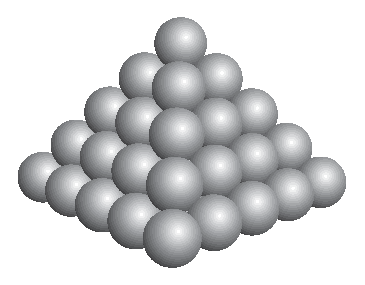
\includegraphics{PS/fcc_small.eps}
  \caption{The face-centered cubic packing}
  \label{fig:fcc}
\end{figure}


The proof of this result is presented in this paper. Here, we
describe the top-level outline of the proof and give references to
the sources of the details of the proof.

\shortversion{An expository account of the proof is contained in
\cite{CH}.  A general reference on sphere packings is \cite{CS}.  A
general discussion of the computer algorithms that are used in the
proof can be found in \cite{algorithm}.  Some speculations on the
structure of a second-generation proof can be found in
\cite{arbeitstagung}. Details of computer calculations can be found
on the internet at \cite{web}.}

\shortversion{The current paper presents an abridged form of the
proof.  The full proof appears in \cite{KC}. Samuel P.
Ferguson\index{Ferguson} has made important contributions to this
proof.  His University of Michigan thesis gives the proof of a
difficult part of the proof \cite{thesis}.  A key \chap\
(\Chap~\ref{sec:scoring}) of this paper is coauthored with
Ferguson.\index{Ferguson}}


By a {\it packing}, we mean an arrangement of congruent balls that
are nonoverlapping in the sense that the interiors of the balls are
pairwise disjoint. Consider a \index{packing} packing of congruent
balls in Euclidean three space. There is no harm in assuming that
all the balls have unit radius. The density of a packing does not
decrease when balls are added to the packing. Thus, to answer a
question about the greatest possible density we may add
nonoverlapping balls until there is no room to add further balls.
Such a packing will be said to be {\it saturated}.
%
 \index{saturated}
 \index{overlap}

Let $\Lambda$ be the set of centers of the balls in a
\index{saturated} saturated packing. Our choice of radius for the
balls implies that any two points in $\Lambda$ have distance at
least $2$ from each other. We call the points of $\Lambda$ {\it
\index{vertex} vertices}.  Let $B(x,r)$ denote the closed ball in
Euclidean three space at center $x$ and radius $r$. Let
$\delta(x,r,\Lambda)$ be the finite density, defined as the ratio
of the volume of $B(x,r,\Lambda)$ to the volume of $B(x,r)$, where
$B(x,r,\Lambda)$ is defined as the intersection with $B(x,r)$ of
the union of all balls in the packing. Set $\Lambda(x,r) = \Lambda
\cap B(x,r)$.\index{ZZdelta@$\delta(x,r,\Lambda)$}

Recall that the \index{Voronoi cell} Voronoi cell
$\Omega(v)=\Omega(v,\Lambda)$\index{ZZzomega@$\Omega(v)$} around a
vertex $v\in \Lambda$ is the set of points closer to $v$ than to
any other ball center. The volume of each Voronoi cell in the
face-centered cubic packing is $\sqrt{32}$.  This is also the
volume of each Voronoi cell in the hexagonal-close packing.

\begin{definition}\label{def:negligible}
Let $A:\Lambda\to\R$ be a function.  We say that $A$\index{Az@$A$}
is
  {\it negligible\/}\index{negligible}
if there is a constant $C_1$ such that for all $r\ge1$ and all
$x\in\ring{R}^3$, we have
   $$\sum_{v\in\Lambda(x,r)} A(v) \le C_1 r^2.$$
We say that the function $A:\Lambda\to\R$ is
  {\it fcc-compatible\/}\index{fcc-compatible}
if for all $v\in\Lambda$ we have the inequality
$$\sqrt{32}\le \op{vol}(\Omega(v)) + A(v).$$
\end{definition}

The value $\op{vol}(\Omega(v)) + A(v)$ may be interpreted as a
{\it corrected\/} volume\index{corrected volume} of the Voronoi
cell. Fcc-compatibility asserts that the corrected volume of the
Voronoi cell is always at least the volume of the Voronoi cells in
the face-centered cubic and hexagonal-close packings.




\begin{lemma}
\label{lemma:deltabound} If there exists a \index{negligible}
negligible \index{fcc-compatible} fcc-compatible function
$A:\Lambda\to\R$ for a saturated packing $\Lambda$, then there
exists a constant $C$ such that for all $r\ge1$ and all
$x\in\ring{R}^3$, we have
    $$
    \delta(x,r,\Lambda)
    \le \pi/\sqrt{18} + C/r.
    $$
The constant $C$ depends on $\Lambda$ only through the constant
$C_1$.
\end{lemma}



\begin{proof}
The numerator $\op{vol}\, B(x,r,\Lambda)$ of $\delta(x,r,\Lambda)$
is at most the product of the volume of a ball $4\pi/3$ with the
number $|\Lambda(x,r+1)|$ of balls intersecting $B(x,r)$.  Hence
    \begin{equation}
    \op{vol}\, B(x,r,\Lambda) \le |\Lambda(x,r+1)| 4\pi/3.
    \label{eqn:Abound}
    \end{equation}

In a saturated packing each Voronoi cell is contained in a ball of
radius $2$ centered at the {\it center} of the cell.  The volume
of the ball $B(x,r+3)$ is at least the combined volume of Voronoi
cells whose center lies in the ball $B(x,r+1)$. This observation,
combined with fcc-compatibility and negligibility, gives
    \begin{equation}
    \begin{split}
    \sqrt{32}|\Lambda(x,r+1)|
    &\le \sum_{v\in\Lambda(x,r+1)} (A(v) +
    \op{vol}(\Omega(v))) \\
    &\le C_1 (r+1)^2 + \op{vol}\,B(x,r+3) \\
    &\le C_1 (r+1)^2 + (1+3/r)^3 \op{vol}\,B(x,r)
    \label{eqn:Bbound}
    \end{split}.
    \end{equation}
Recall that $\delta(x,r,\Lambda)=
\op{vol}\,B(x,r,\Lambda)/\op{vol}\,B(x,r)$. Divide Inequality
\ref{eqn:Abound} through by $\op{vol}\,B(x,r)$.  Use
Inequality~\ref{eqn:Bbound} to eliminate $|\Lambda(x,r+1)|$ from the
resulting inequality.  This gives
    $$\delta(x,r,\Lambda)
        \le \frac{\pi}{\sqrt{18}} (1+3/r)^3 + C_1 \frac{(r+1)^2}{r^3\sqrt{32}}.
    $$
The result follows for an appropriately chosen constant $C$.
\end{proof}

An analysis of the preceding proof shows that fcc-compatibility
leads to the particular value $\pi/\sqrt{18}$ in the statement of
Lemma~\ref{lemma:deltabound}.  If fcc-compatibility were to be
dropped from the hypotheses, any negligible function $A$ would
still lead to an upper bound $4\pi/(3L)$ on the density of a
packing, expressed as a function of a lower bound $L$ on all
$\op{vol}\,\Omega(v)+A(v)$.


\begin{remark} \label{remark:precise}
We take the precise meaning of the Kepler conjecture to be a bound
on the essential supremum of the function $\delta(x,r,\Lambda)$ as
$r$ tends to infinity. Lemma \ref{lemma:deltabound} implies that the
essential supremum of $\delta(x,r,\Lambda)$ is bounded above by
$\pi/\sqrt{18}$, provided a negligible fcc-compatible function can
be found.  The strategy will be to define a negligible function, and
then to solve an optimization problem in finitely many variables to
establish that it is fcc-compatible.
\end{remark}

\Chap~\ref{sec:compact} defines a compact topological space
$\op{DS}$ (the space of decomposition stars
\ref{def:decomposition-star}) and a continuous function $\sigma$
on that space, which is directly related to packings.

If $\Lambda$ is a saturated packing, then there is a geometric
object $D(v,\Lambda)$ constructed around each vertex
$v\in\Lambda$. $D(v,\Lambda)$ depends on $\Lambda$ only through
the vertices in $\Lambda$ that are at most a constant distance
away from $v$.  That constant is independent of $v$ and $\Lambda$.
The objects $D(v,\Lambda)$ are called {\it decomposition stars},
and the space of all decomposition stars is precisely $\op{DS}$.
\index{decomposition star} Section~\ref{sec:cell-ds} shows that
the data in a decomposition star is sufficient to determine a
Voronoi cell\index{Voronoi cell}
$\Omega(D)$\index{ZZzomega@$\Omega(D)$} for each $D\in\op{DS}$.
The same section shows that the Voronoi cell attached to $D$ is
related to the Voronoi cell of $v$ in the packing by relation
   $$\op{vol}\,\Omega(v) = \op{vol}\,\Omega(D(v,\Lambda)).$$
\Chap~\ref{sec:scoring} defines a continuous real-valued function
$A_0:\op{DS}\to\ring{R}$ that assigns a ``weight'' to each
decomposition star.  The topological space $\op{DS}$ embeds into a
finite dimensional Euclidean space. The reduction from an infinite
dimensional to a finite dimensional problem is accomplished by the
following results.

\begin{theorem}\label{lemma:negligible'}
For each saturated packing $\Lambda$, and each $v\in\Lambda$,
there is a decomposition star $D(v,\Lambda)\in\op{DS}$ such that
the function $A:\Lambda\to\ring{R}$ defined by
   $$A(v)= A_0(D(v,\Lambda))$$
is negligible for $\Lambda$.
\end{theorem}

This is proved as Theorem~\ref{lemma:negligible}.  The main object
of the proof is then to show that the function $A$ is
fcc-compatible. This is implied by the inequality (in a finite
number of variables)
      \begin{equation}
      \sqrt{32}\le\op{vol}\,\Omega(D)+ A_0(D),
      \label{eqn:32}
      \end{equation}
for all $D\in\op{DS}$.

In the proof it is convenient to reframe this optimization problem
by composing it with a linear function.  The resulting continuous
function $\sigma:\op{DS}\to\ring{R}$ is called the
  {\it scoring function}, or {\it score}.
  \index{scoring function}\index{score}

Let $\dtet$\index{ZZdeltatet@$\dtet$} be the packing density of a
regular tetrahedron. That is, let $S$ be a regular tetrahedron of
edge length $2$.  Let $B$ the part of $S$ that lies within
distance $1$ of some vertex. Then $\dtet$ is the ratio of the
volume of $B$ to the volume of $S$. We have $\dtet = \sqrt{8}
\arctan(\sqrt{2}/5)$.

Let $\doct$\index{ZZdeltaoct@$\doct$} be the packing density of a
regular octahedron of edge length $2$, again constructed as the
ratio of the volume of points within distance $1$ of a vertex to
the volume of the octahedron.

The density of the face-centered cubic packing is a weighted average of
these two ratios
    $$\frac{\pi}{\sqrt{18}} = \frac{\dtet}{3} + \frac{2 \doct}{3}.$$
This determines the exact value of $\doct$ in terms of $\dtet$. We have
$\doct \approx 0.72$.

In terms of these quantities,
\begin{equation}
    \sigma(D) = -4 \doct (\op{vol}(\Omega(D)) + A_0(D)) +
    \frac{16\pi}{3}.
\end{equation}

\begin{definition}\label{def:pt}
We define\index{point}\index{pt} the constant
   $$\pt = 4\arctan(\sqr2/5) - \pi/3.$$
Its value is approximately $pt \approx 0.05537.$  Equivalent
expressions for $\pt$ are
    $$
    \pt = \sqrt2 \dtet - \frac{\pi}{3} = -2 (\sqrt2 \doct -
    \frac{\pi}{3}).
    $$
\end{definition}

%The following conjecture is made in \cite{formulation}

In terms of the scoring function $\sigma$, the optimization
problem in a finite number of variables (Inequality~\ref{eqn:32})
takes the following form. The proof of this inequality is a
central concern in this paper.

\begin{theorem}[Finite dimensional reduction]\label{theorem:sigma}
The maximum of $\sigma$ on the topological space $\op{DS}$ of all
decomposition stars is the constant $8\,\pt\approx 0.442989$.
\end{theorem}

\begin{remark} The Kepler conjecture is an optimization problem in
an infinite number of variables (the coordinates of the points of
$\Lambda$).   The maximization of $\sigma$ on $\op{DS}$ is an
optimization problem in a finite number of variables.
Theorem~\ref{theorem:sigma} may be viewed as a finite-dimensional
reduction of the Kepler conjecture.
\end{remark}
\bigskip


Let $t_0=1.255$ ($2t_0 = 2.51$).\index{tZ0@$t_0=1.255$}  This is a
parameter that is used for truncation throughout this paper.
%
 \index{truncation parameter}

Let $U(v,\Lambda)$
 %
 \index{UZ@$U(v,\Lambda)$}
 \index{UZ@$U(D)$}
be the set of vertices in $\Lambda$ at nonzero distance at most
$2t_0$ from $v$.  From $v$ and a decomposition star $D(v,\Lambda)$
it is possible to recover $U(v,\Lambda)$, which we write as $U(D)$.
We can completely characterize the decomposition stars at which the
maximum of $\sigma$ is attained.

\begin{theorem}
\label{theorem:sharp} Let $D$ be a decomposition star at which the
function $\sigma:\op{DS}\to\ring{R}$ attains its maximum. Then the
set $U(D)$ of vectors at distance at most $2t_0$ from the center
has cardinality $12$. Up to Euclidean motion, $U(D)$ is one of two
arrangements: the kissing arrangement of the $12$ balls around a
central ball in the face-centered cubic
packing\index{face-centered cubic} or the kissing arrangement of
$12$ balls in the hexagonal-close packing\index{hexagonal-close
packing}.
\end{theorem}

There is a complete description of all packings in which every
sphere center is surrounded by $12$ others in various combinations
of these two patterns. All such packings are built from parallel
layers of the $A_2$ lattice.  (The $A_2$ lattice formed by
equilateral triangles, is the optimal packing in two dimensions.)
See \longversion{\Part~\ref{part:intro}}\shortversion{\cite{KC}}.


\section{Basic Concepts in the Proof}
\label{sec:outline}


To prove Theorems~\ref{theorem:kepler}, \ref{theorem:sigma}, and
\ref{theorem:sharp}, we wish to show that there is no
counterexample.  In particular, we wish to show that there is no
decomposition star $D$ with value $\sigma(D)
> 8\,\pt$.  We reason by contradiction, assuming the existence of
such a decomposition star.  With this in mind, we call $D$ a {\it
contravening decomposition star},\index{contravening} if
    $$\sigma(D)\ge 8\,\pt.$$
In much of what follows we will tacitly assume that every decomposition
star under discussion is a contravening one.  Thus, when we say that no
decomposition stars exist with a given property, it should be
interpreted as saying that no such contravening decomposition stars
exist.\index{decomposition star!contravening}

To each contravening decomposition star $D$, we associate a
(combinatorial) plane graph $G(D)$.  A restrictive list of
properties of plane graphs is described in
Section~\ref{sec:graphproperty}. Any plane graph satisfying these
properties is said to be {\it tame}. All \index{tame} tame plane
graphs have been classified. There are several thousand, up to
isomorphism.  The list appears in \cite{web}.  We refer to this
list as the {\it archival list}\index{archival list of graphs} of
plane graphs.


A few of the tame plane graphs are of particular interest. Every
decomposition star attached to the face-centered cubic packing gives the
same plane graph (up to isomorphism).  Call it $G_{fcc}$.  Likewise,
every decomposition star attached to the hexagonal-close packing gives
the same plane graph $G_{hcp}$.
%Let $\op{DS}_{crit}$ be the set of
%decomposition stars $D$ such that the set $U(D)$ of vertices is the
%kissing arrangement of the $12$ balls around a central ball in the
%face-centered cubic or hexagonal-close packing.
\begin{figure}[htb]
  \centering
  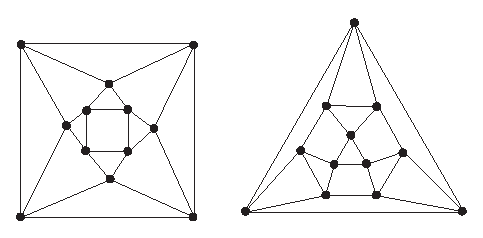
\includegraphics{PS/gfcchcp.eps}
  \caption{The plane graphs $G_{fcc}$ and $G_{hcp}$}
  \label{fig:gfcchcp}
\end{figure}

There is one more tame plane graph that is particularly troublesome.
It is the graph $G_{pent}$\index{pentahedral prism} obtained from
the pictured configuration of twelve balls tangent to a given
central ball (Figure \ref{fig:pentahedral}). (Place a ball at the
north pole, another at the south pole, and then form two pentagonal
rings of five balls.) This case requires individualized attention.
S. Ferguson\index{Ferguson} proves the following theorem in
\shortversion{his thesis \cite{thesis}.}
\longversion{\Part~\ref{part:ferguson}.}

\begin{theorem} [Ferguson] \label{lemma:ferguson}
There are no contravening decomposition stars $D$ whose associated
plane graph is isomorphic to $G_{pent}$.
\end{theorem}


\begin{figure}[htb]
  \centering
  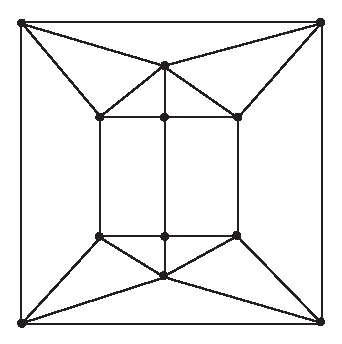
\includegraphics{PS/gpent.eps}
  \caption{The plane graph $G_{pent}$}\index{pentahedral prism}
   of the pentahedral prism.
  \label{fig:pentahedral}
\end{figure}

\section{Logical Skeleton of the Proof}
\label{sec:logic}

Consider the following six claims.  Eventually we will give a
proof of all six statements.  First, we draw out some of their
consequences.  The main results (Theorems~\ref{theorem:kepler},
\ref{theorem:sigma}, and \ref{theorem:sharp}) all follow from
these claims.

\begin{claim}\label{claim-A}
If the maximum of the function $\sigma$ on $\op{DS}$ is $8\,\pt$,
then for every saturated packing $\Lambda$ there exists a
negligible fcc-compatible function $A$.
\end{claim}

\begin{claim}\label{claim-B}
Let $D$ be a contravening decomposition star. Then its plane graph
$G(D)$ is tame.
\end{claim} %\ref{theorem:contravene} in kepler.tex

\begin{claim}\label{claim-C}
If a plane graph is tame, then it is isomorphic to one of the
several thousand plane graphs that appear in the archival list of
plane graphs.
\end{claim} %\ref{theorem:classification} in kepler.tex

\begin{claim}\label{claim-D}
If the plane graph of a contravening
decomposition star is isomorphic to one in the archival list of
plane graphs, then it is isomorphic to one of the following three
plane graphs: $G_{pent}$, $G_{hcp}$, or $G_{fcc}$.
\end{claim} %\label{lemma:fcc-hcp-pent} in linprog.tex

\begin{claim}\label{claim-E}
There do not exist any contravening decomposition stars
$D$ whose associated graph is isomorphic to $G_{pent}$.
\end{claim} %\label{lemma:ferguson} in form.tex

\begin{claim}\label{claim-F}
Contravening decomposition stars exist.
If $D$ is a contravening
decomposition star, and if the plane graph of $D$ is isomorphic to
$G_{fcc}$ or $G_{hcp}$, then $\sigma(D) = 8\,\pt$.  Moreover, up
to Euclidean motion, $U(D)$ is the kissing arrangement of the $12$
balls around a central ball in the face-centered cubic packing or
the kissing arrangement of $12$ balls in the hexagonal-close
packing.
\end{claim} %\label{lemma:local-optimality} in local_opt.tex

Next, we state some of the consequences of these claims.

\begin{lemma}\label{lemma:claim-fcc-graph}
Assume Claims~\ref{claim-B}, \ref{claim-C}, \ref{claim-D}, and
\ref{claim-E}. If $D$ is a contravening decomposition star, then
its plane graph $G(D)$ is isomorphic to $G_{hcp}$ or $G_{fcc}$.
\end{lemma}

\begin{proof} Assume that $D$ is a contravening decomposition
star.  Then its plane graph is tame, and consequently appears on
the archival list of plane graphs.  Thus, it must be isomorphic to
one of $G_{fcc}$, $G_{hcp}$, or $G_{pent}$.  The final graph is
ruled out by Claim~\ref{claim-E}.
\end{proof}

\begin{lemma}\label{lemma:claim-sigma}
Assume Claims~\ref{claim-B}, \ref{claim-C}, \ref{claim-D},
\ref{claim-E}, and \ref{claim-F}. Then Theorem~\ref{theorem:sigma}
holds.
\end{lemma}

\begin{proof}
By Claim~\ref{claim-F} and Lemma~\ref{lemma:claim-fcc-graph}, the
value $8\,\pt$ lies in the range of the function $\sigma$ on
$\op{DS}$.   Assume for a contradiction that there exists a
decomposition star $D\in \op{DS}$ that has $\sigma(D)>8\,\pt$. By
definition, this is a contravening star. By
Lemma~\ref{lemma:claim-fcc-graph}, its plane graph is isomorphic
to $G_{hcp}$ or $G_{fcp}$.  By Claim~\ref{claim-F},
$\sigma(D)=8\,\pt$, in contradiction with $\sigma(D)>8\,\pt$.
\end{proof}

\begin{lemma}\label{lemma:claim-sharp}
Assume Claims~\ref{claim-B}, \ref{claim-C}, \ref{claim-D},
\ref{claim-E}, and \ref{claim-F}.  Then
Theorem~\ref{theorem:sharp} holds.
\end{lemma}

\begin{proof}  By Theorem~\ref{theorem:sigma}, the maximum of
$\sigma$ on $\op{DS}$ is $8\,\pt$.  Let $D$ be a decomposition
star at which the maximum $8\,\pt$ is attained.  Then $D$ is a
contravening star. Lemma~\ref{lemma:claim-fcc-graph} implies that
the plane graph is isomorphic to $G_{hcp}$ or $G_{fcc}$.  The
hypotheses of Claim~\ref{claim-F} are satisfied.  The conclusion
of Claim~\ref{claim-F} is the conclusion of
Theorem~\ref{theorem:sharp}.
\end{proof}

\begin{lemma}
Assume Claims~\ref{claim-A}--\ref{claim-F}. Then the Kepler
conjecture (Theorem~\ref{theorem:kepler}) holds.
\end{lemma}

\begin{proof} As pointed out in Remark~\ref{remark:precise}, the precise
meaning of the Kepler conjecture is for every saturated packing
$\Lambda$, the essential supremum of $\delta(x,r,\Lambda)$ is at
most $\pi/\sqrt{18}$.

Let $\Lambda$ be the set of centers of a saturated packing.  Let
$A:\Lambda \to \ring{R}$ be the negligible, fcc-compatible
function provided by Claim~\ref{claim-A} (and
Lemma~\ref{lemma:claim-sigma}). By Lemma~\ref{lemma:deltabound},
the function $A$ leads to a constant $C$ such that for all $r\ge
1$ and all $x\in \ring{R}^3$, the density $\delta(x,r,\Lambda)$
satisfies
   $$\delta(x,r,\Lambda) \le \pi/\sqrt{18} + C/r.$$
This implies that the essential supremum of $\delta(x,r,\Lambda)$
is at most $\pi/\sqrt{18}$.
\end{proof}

\begin{remark}
One other theorem (Theorem~\ref{lemma:negligible'}) was stated
without proof in Section~\ref{sec:statement}.  This result was
placed there to motivate the other results.  However, it is not an
immediate consequence of Claims~\ref{claim-A}--\ref{claim-F}.  Its
proof appears in Theorem~\ref{lemma:negligible}.
\end{remark}

\section{Proofs of the Central Claims}

The previous section showed that the main results in the
introduction (Theorems~\ref{theorem:kepler}, \ref{theorem:sigma},
and \ref{theorem:sharp}) follow from six claims. This section
indicates where each of these claims is proved, and mentions a few
facts about the proofs.

Claim~\ref{claim-A} is proved in Theorem~\ref{lemma:exista}.
Claim~\ref{claim-B} is proved in Theorem~\ref{theorem:contravene}.
Claim~\ref{claim-C}, the classification of tame graphs, is proved in
Theorem~\ref{theorem:classification}. By the classification of such
graphs, this reduces the proof of the Kepler conjecture to the
analysis of the decomposition stars attached to the finite explicit
list of tame plane graphs.  We will return to Claim~\ref{claim-D} in
a moment.  Claim~\ref{claim-E} is Ferguson's thesis, cited as
Theorem~\ref{lemma:ferguson}.

Claim~\ref{claim-F} is the local optimality of the face-centered
cubic and hexagonal close packings.   In
\Chap~\ref{sec:local-opt}, the necessary local analysis is carried
out to prove Claim~\ref{claim-F} as
Corollary~\ref{lemma:local-optimality2}.

%\begin{lemma}
%A decomposition star whose plane graph is $G_{fcc}$ or $G_{hcp}$ has
%    $$\sigma(D) \le 8\,\pt,$$
%with equality precisely when the decomposition star belongs to
%$\op{DS}_{crit}$. \end{lemma}

%In light of this result, we prove Theorem \ref{theorem:sigma} and
%Theorem \ref{theorem:sharp} by proving that any decomposition star
%whose graph is tame and not equal to $G_{fcc}$ or $G_{hcp}$ is not
%contravening.

Now we return to Claim~\ref{claim-D}. This claim is proved as
Theorem~\ref{lemma:fcc-hcp-pent}.  The idea of the proof is the
following.  Let $D$ be a contravening decomposition star with
graph $G(D)$. We assume that the graph $G(D)$ is not isomorphic to
$G_{fcc}$, $G_{hcp}$, $G_{pent}$ and then prove that $D$ is not
contravening. This is a case-by-case argument, based on the
explicit archival list of plane graphs.

To eliminate these remaining cases, more-or-less generic arguments
can be used.  A linear program is attached to each tame graph $G$.
The linear program can be viewed as a linear relaxation of the
nonlinear optimization problem of maximizing $\sigma$ over all
decomposition stars with a given tame graph $G$. Because it is
obtained by relaxing the constraints on the nonlinear problem, the
maximum of the linear problem is an upper bound on the maximum of
the original nonlinear problem. Whenever the linear programming
maximum is less than $8\,\pt$, it can be concluded that there is
no contravening decomposition star with the given tame graph $G$.
This linear programming approach eliminates most tame graphs.

When a single linear program fails to give the desired bound, it
is broken into a series of linear programming bounds, by branch
and bound techniques.  For every tame plane graph $G$ other than
$G_{hcp}$, $G_{fcc}$, and $G_{pent}$,\index{pentahedral prism} we
produce a series of linear programs that establish that there is
no contravening decomposition star with graph $G$.

The \paper~is organized in the following way.
\Chaps~\ref{sec:construction} through \ref{sec:scoring} introduce
the basic definitions.  \Chap~\ref{sec:scoring} gives a proof of
Claim~\ref{claim-A}. \Chap~\ref{sec:local-opt} proves
Claim~\ref{claim-F}. \longversion{\Chaps~\ref{sec:fine} through
\ref{sec:fb} present the fundamental estimates.}
\Chaps~\ref{sec:def-and-class} through
\ref{sec:proof-classification} give a proof of Claim~\ref{claim-C}.
\Chaps~\ref{sec:startame} through \ref{sec:weight} give a proof of
Claim~\ref{claim-B}. \Chaps~\ref{sec:linearprogram} through
\ref{sec:branchbound} give a proof of Claim~\ref{claim-D}.
Claim~\ref{claim-E} (Ferguson's thesis) \shortversion{is to be
published as a separate paper.} \longversion{appears in
\Part~\ref{part:ferguson}.}


\chapter{Construction of the $Q$-system}
\label{sec:construction}

%This chapter has been written in a way that to be logically independent
%of the other papers in this series.  However, some of the results are
%technical lemmas that are required in other chapters. Thus, some of the
%results in this chapter may seem to be lacking in motivation. For
%motivation and a top-level view of the proof of the Kepler conjecture,
%the reader should consult Chapter~\ref{sec:overview}.  The reader is
%strongly encouraged to read that chapter first.  The paper \cite{CH}
%also gives an informal introduction to the proof that is less
%technically demanding than this paper.

%The ``program" to prove the Kepler conjecture has been changed somewhat
%from some of my earlier papers (see \cite{part1} and \cite{part2}).
%Hence, we do not rely on any definitions or ``program-related'' theorems
%from these papers.  However, we make free use of statements in pure
%geometry from those papers, when it is perfectly clear that these
%statements do not depend on any program-specific definitions or results.
%All program-specific results are proved from scratch in this paper,
%even when the proof is nearly identical to a proof found in one of these
%earlier papers.

It is useful to separate the parts of space of relatively high
packing density from the parts of space with relatively low packing
density.  The $Q$-system, which is developed in this \chap, is a
crude way of marking off the parts of space where the density is
potentially high.  The $Q$-system is a collection of simplices whose
vertices are points of the packing $\Lambda$. The $Q$-system is
reminiscent of the Delaunay decomposition, in the sense of being a
collection of simplices with vertices in $\Lambda$.  In fact, the
$Q$-system is the remnant of an earlier approach to the Kepler
conjecture that was based entirely on the Delaunay decomposition
(see \cite{remarks}).  However, the $Q$-system differs from the
Delaunay decomposition in crucial respects.  The most fundamental
difference is that the $Q$-system, while consisting of
nonoverlapping simplices, does not partition all of space.

This \chap\ defines the set of simplices in the $Q$-system and
proves that they do not overlap.  In order to prove that the
simplices in the $Q$-system do not overlap,  we develop a long
series of lemmas that study the geometry of intersections of
various edges and simplices.  At the end of this \chap, we give
the proof that the simplices in the $Q$-system do not overlap.

\section{Description of the $Q$-system}
\label{sec:Q-describe}



Fix a packing of balls of radius $1$. We identify the packing with
the set $\Lambda$ of its centers.  A packing is thus a subset
$\Lambda$ of $\ring{R}^3$ such that for all $v,w\in\Lambda$,
$|v-w|<2$ implies $v=w$. The centers of the balls are called {\it
\index{vertex} vertices}. The term `vertex' will be reserved for
this technical usage.  A packing is said to be {\it
\index{saturated} saturated\/} if for every $x\in\ring{R}^3$,
there is some $v\in\Lambda$ such that $|x-v|<2$. Any packing is a
subset of a saturated packing. We assume that $\Lambda$ is
saturated. The set $\Lambda$ is countably infinite.

\begin{definition}  We define the {\it truncation parameter}
\index{truncation parameter ($t_0=1.255$)} to be the constant
$t_0=1.255$. It is used throughout. Informal arguments that led to
this choice of constant are described in
\longversion{\Part~\ref{part:intro}}\shortversion{\cite{KC}}.
\end{definition}

Precise constructions that rely on the truncation parameter $t_0$
will appear below.  We will regularly intersect Voronoi cells with
balls of radius $t_0$ to obtain lower bounds on their volumes.  We
will regularly disregard vertices of the packing that lie at
distance greater than $2t_0$ from a fixed $v\in\Lambda$ to obtain
a finite subset of $\Lambda$ (a finite cluster of balls in the
packing) that is easier to analyze than the full packing
$\Lambda$.

The truncation parameter is the first of many decimal constants
that appear. Each decimal constant is an exact rational value,
e.g. $2t_0 = 251/100$.  They are not to be regarded as
approximations of some other value.

\begin{definition}
A {\it quasi-regular\/} triangle\index{quasi-regular triangle} is
a set $T\subset \Lambda$ of three vertices such that if $v,w\in T$
then $|w-v|\le2t_0$. \end{definition}

\begin{definition}
A \index{simplex} simplex\index{simplex} is a set of four
vertices.
%The
%edge-lengths of a simplex $S$ are the lengths $|w-v|$ for $w,v\in
%S$ and $w\ne v$.
A {\it quasi-regular\/} tetrahedron is a simplex $S$ such that if
$v,w\in S$ then $|w-v|\le 2t_0$. A {\it quarter\/} is a simplex
whose edge lengths $y_1,\ldots,y_6$ can be ordered to satisfy
$2t_0\le y_1\le\sqr8$, $2\le y_i\le 2t_0$, $i=2,\ldots,6$. If a
quarter satisfies the strict inequalities $2t_0< y_1< \sqrt8$,
then we say that it is a strict quarter. We call the longest edge
$\{v,w\}$ of a quarter its {\it \index{diagonal} diagonal\/}. When
the quarter is strict, we also say that its diagonal is strict.
When the quarter has a distinguished vertex, the quarter is {\it
upright\/} if the distinguished vertex is an endpoint of the
diagonal, and {\it flat\/} otherwise.
\end{definition}
\index{quarter!strict} \index{quarter!upright}
\index{quarter!flat} \index{quasi-regular}
\index{quasi-regular!triangle} \index{quasi-regular!tetrahedron}

At times, we identify a simplex with its convex hull. We will say,
for example, that the circumcenter of a simplex is contained in
the simplex to mean that the circumcenter is contained in the
convex hull of the four vertices.  Similar remarks apply to
triangles, quasi-regular tetrahedra, quarters, and so forth.  We
will write $|S|$ for the convex hull of $S$ when we wish to be
explicit about the distinction between $|S|$ and its set of
extreme points.

When we wish to give an order on an edge, triangle, simplex, etc.
we present the object as an ordered tuple rather than a set. Thus,
we refer to both $(v_1,\ldots,v_4)$ and $\{v_1,\ldots,v_4\}$ as
simplices, depending on the needs of the given context.

\begin{definition}\index{overlap}
Two manifolds with boundary {\it overlap\/} if their interiors
intersect.
\end{definition}


\begin{definition}  A set $O$ of six vertices is
called a {\it quartered \index{octahedron} octahedron}, if there are
four pairwise nonoverlapping strict quarters $S_1,\ldots,S_4$ all
having the same diagonal, such that $O$ is the union of the four
sets $S_i$ of four vertices.  (It follows easily that the strict
quarters $S_i$ can be given a cyclic order with respect to which
each strict quarter $S_i$ has a face in common with the next, so
that a quartered octahedron is literally a octahedron that has been
partitioned into four quarters.)
\end{definition}

\begin{remark}\label{def:oct-order}
A quartered octahedron may have more than one diagonal of length
less than $\sqr8$, so its decomposition into four strict quarters
need not be unique.  The choice of diagonal has no particular
importance.  Nevertheless, to make things canonical, we pick the
diagonal of length less than $\sqrt8$ with an endpoint of smallest
possible value with respect to the lexicographical ordering on
coordinates; that is, with respect to the ordering $(y_1,y_2,y_3)
< (y_1',y_2',y_3')$, if $y_i=y'_i$, for $i=1,\ldots,k$, and
$y_{k+1}<y'_{k+1}$.  This selection rule for diagonals is fully
translation invariant in the sense that if one octahedron is a
translate of another (whether or not they belong to the same
saturated packing), then the selected diagonal of one is a
translate of the selected diagonal of the other.
\end{remark}

%An {\it octahedral ordering} of a saturated packing is a function
%that assigns a choice of diagonal of length less than $\sqrt8$ to
%each quartered octahedron.  We fix once and for all an octahedral
%ordering of every saturated packing.  We may assume that the
%choice is fully translation invariant in the sense that if
%$\Lambda$ and $\Lambda'$ are any two saturated packings (not
%necessarily distinct) and one contains an octahedron that is a
%translation of an octahedron in the other, then the choice of
%diagonal in one is a translation of the choice in the other.  One
%such (translation invariant) ordering would be the diagonal with
%an endpoint with the smallest possible value with respect to the
%lexicographical ordering on the coordinates.


%This choice of distinguished diagonal is entirely immaterial for
%the proof of the Kepler conjecture.  However, we wish to assert
%that certain constructions are canonical.  For that reason, we
%prefer to avoid basing our choice of diagonal on an arbitrary
%well-ordering of the diagonals. However, there are various rules
%for picking out one diagonal that do not involved any arbitrary
%choices and that rely instead on suitable lexicographical
%orderings of the edge-lengths in the octahedron. A canonical rule
%will be translation and rotation invariant.  Such a rule can be
%designed so that it always selects a diagonal of length less than
%$\sqrt8$ whenever such a diagonal exists.  Of course, any
%canonical rule based on edge-lengths will be invariant under the
%group of isometries of the octahedron, any cannot select a
%distinguished diagonal from a regular octahedron. However, a
%regular octahedron with sides at least $2$ has diagonals of length
%at least $\sqrt8$, and it therefore not a quartered octahedron. To
%avoid excess pedantry, we will not spell out a rule in detail.
% FALSE! Cannot always break the symmetry between the two shorter diags.



\begin{definition} \label{def:anchor}
If $\{v_1,v_2\}$ is an edge of length between $2t_0$ and $\sqr8$,
we say that a vertex $v$ $(\ne v_1,v_2)$ is an {\it \index{anchor}
anchor\/} of $\{v_1,v_2\}$ if its distances to $v_1$ and $v_2$ are
at most $2t_0$.
%
\end{definition}

The two vertices of a quarter that are not on the diagonal are
anchors of the diagonal, and the diagonal may have other anchors
as well.

\begin{definition}\label{def:q-system}
Let $\CalQ$ be the set of quasi-regular tetrahedra and strict
quarters, enumerated as follows. This set is called the
$Q$-system.  It is canonically associated with a saturated packing
$\Lambda$.  (The $Q$ stands for quarters and quasi-regular
tetrahedra.)
%
  \index{Q-system@$Q$-system}


\begin{enumerate}
   \item All quasi-regular tetrahedra.
   \item Every strict quarter such that none of the quarters along
   its diagonal overlaps any other
   quasi-regular tetrahedron or strict quarter.
   \item Every strict quarter whose diagonal has four or more
   anchors, as long as there are not exactly four anchors arranged
   as a quartered
   octahedron.
   \item The fixed choice of four strict quarters in each
   quartered octahedron.
   %\item Assume a strict quarter does not overlap a quasi-regular tetrahedron,
   %overlaps at least one other strict quarter,
   % and is not part of a quartered octahedron.  Of these, we include
   %\begin{enumerate}
   \item Every strict quarter $\{v_1,v_2,v_3,v_4\}$ whose diagonal
      $\{v_1,v_3\}$ has exactly three anchors $v_2$, $v_4$, $v_5$ provided that
      the following hold (for some choice of indexing).
      (a) $\{v_2,v_5\}$ is a strict diagonal
      with exactly three anchors: $v_1$, $v_3$, $v_4$.
      (b) $d_{24}+d_{25}>\pi$, where $d_{24}$ is the dihedral angle
       of the simplex $\{v_1,v_3,v_2,v_4\}$ along the edge $\{v_1,v_3\}$
       and $d_{25}$ is the dihedral angle of the simplex
       $\{v_1,v_3,v_2,v_5\}$ along the edge $\{v_1,v_3\}$.
       %The sum of the dihedral
       %  angles $\dih(v_1,v_3,v_2,v_4)+\dih(v_1,v_3,v_2,v_5)$ is
       %  greater than $\pi$.
   %\end{enumerate}
\end{enumerate}
No other quasi-regular tetrahedra or strict quarters are included
in the $Q$-system $\CalQ$.
\end{definition}


The following theorem is the main result of this \chap.

\begin{theorem}\label{thm:nonoverlap}
For every saturated packing, there exists a uniquely determined
$Q$-system.  Distinct simplices in the $Q$-system have disjoint
interiors.
\end{theorem}

While proving the theorem, we give a complete classification of
the various ways in which one quasi-regular tetrahedron or strict
quarter can overlap another.

Having completed our primary purpose of showing that the simplices
in the $Q$-system do not overlap, we state the following small
lemma. It is an immediate consequence of the definitions, but
which is nonetheless useful in the \chaps\ that follow.

\begin{lemma} \label{lemma:diags-engulf}
If one quarter along a diagonal lies in the $Q$-system, then all
quarters along the diagonal lie in the $Q$-system.
\end{lemma}

\begin{proof} This is true by construction.  Each of the defining properties
of a quarter in the $Q$-system is true for one quarter along a
diagonal if and only if  it is true of all quarters along the
diagonal.
\end{proof}


\section{Geometric Considerations}
    \label{sec:decomposition}

\begin{remark}  The primary definitions and
constructions of this paper are translation invariant.  That is,
if $\lambda\in\ring{R}^3$ and $\Lambda$ is a saturated packing,
then $\lambda+\Lambda$ is a saturated packing.  If
$A:\Lambda\to\ring{R}$ is a negligible fcc-compatible function for
$\Lambda$, then $\lambda+v\mapsto A(v)$ is a negligible
fcc-compatible function for $\lambda+\Lambda$.  If $\CalQ$ is the
$Q$-system of $\Lambda$, then $\lambda+\CalQ$ is the $Q$-system of
$\lambda+\Lambda$. Because of general translational invariance,
when we fix our attention on a particular $v\in\Lambda$, we will
often assume (without loss of generality) that the coordinate
system is fixed in such a way that $v$ lies at the origin.
\end{remark}

Our simplices are generally assumed to come labeled with a
distinguished vertex, fixed  at the origin. (The origin will
always be at a vertex of the packing.) We number the edges of each
simplex $1,\ldots,6$, so that edges $1$, $2$, and $3$ meet at the
origin, and the edges $i$ and $i+3$ are opposite, for $i=1,2,3$.
(See Figure~\ref{fig:diag11}.)  $S(y_1,y_2,\ldots,y_6)$ denotes a
simplex whose edges have lengths $y_i$, indexed in this way. We
refer to the endpoints away from the origin of the first, second,
and third edges as the first, second, and third vertices.
%
 \index{labels!edge}
 \index{first!edge}

\begin{definition}\label{def:dih}
In general, let $\dih(S)$ be the dihedral angle of a simplex $S$
along its first edge. When we write a simplex in terms of its
vertices $(w_1,w_2,w_3,w_4)$, then $\{w_1,w_2\}$ is understood to
be the first edge.
%
 \index{dih (dihedral angle)}
\end{definition}

\begin{definition}
We define the {\it radial projection\/} of a set $X$ to be the
radial projection $x\mapsto x/|x|$ of $X\setminus{0}$ to the unit
sphere centered at the origin. We say the two sets {\it cross\/}
if their radial projections to the unit sphere
overlap.\index{projection of a set}
%
 \index{cross}
 \index{radial projection}
\end{definition}


\begin{definition}
    \label{def:calE}
If $S$ and $S'$ are nonoverlapping simplices with a shared face $F$,
we define $\CalE(S,S')$ as the distance between the two vertices
(one on $S$ and the other on $S'$) that do not lie on $F$.  We may
express this as a function
   $$\CalE(S,S')=\CalE(S(y_1,\ldots,y_6),y_1',y_2',y_3')$$
of nine variables, where $S=S(y_1,\ldots,y_6)$  and
$S'=S(y_1',y_2',y_3',y_4,y_5,y_6)$, positioned so that $S$ and $S'$
are nonoverlapping simplices with a shared face $F$ of edge-lengths
$(y_4,y_5,y_6)$.   The function of nine variables is defined only
for values $(y_i,y_i')$ for which the simplices $S$ and $S'$ exist.
(Figure~\ref{fig:diag11}).
\end{definition}

\begin{figure}[htb]
  \centering
  \includegraphics{PS/calE.eps}
  \caption{$\CalE$ measures the distance between the vertices at $0$ and $v$.
   The standard indexing of the edges of a simplex
   is marked on the lower simplex.}
  \label{fig:diag11}
\end{figure}

Several lemmas in this paper rely on calculations of lower bounds
to the function $\CalE$ in the special case when the edge between
the vertices $0$ and $v$ passes through the shared face $F$. If
intervals containing $y_1,\ldots,y_6,y_1',y_2',y_3'$ are given,
then lower bounds on $\CalE$ over that domain are generally easy
to obtain.  Detailed examples of calculations of the lower bound
of this function can be found in \cite[Sec. 4]{part1}.

To work one example, we suppose we are asked to give a lower bound
on $\CalE$ when the simplex $S=S(y_1,\ldots,y_6)$ satisfies
$y_i\ge2$ and $y_4,y_5,y_6\le 2t_0$ and
$S'=S(y'_1,y'_2,y'_3,y_4,y_5,y_6)$ satisfies $y'_i\ge2$, for
$i=1,\ldots,3$. Assume that the edge $\{0,v\}$ passes through the
face shared between $S$ and $S'$, and that $|v|<\sqrt8$, where $v$
is the vertex of $S'$ that is not on $S$.  We claim that any pair
$S,S'$ can be deformed by moving one vertex at a time until $S$ is
deformed into $S(2,2,2,2t_0,2t_0,2t_0)$ and $S'$ is deformed into
$S(2,2,2,2t_0,2t_0,2t_0)$.  Moreover, these deformations preserve
the constraints (including that $\{0,v\}$ passes through the shared
face), and is non-increasing in $|v|$.  From the existence of this
deformation, it follows that the original $|v|$ satisfies
   $$|v| \ge \CalE(S(2,2,2,2t_0,2t_0,2t_0),2,2,2).$$

We produce the deformation in this case as follows. We define the
{\it pivot\/} of a vertex $v$ with respect to two other vertices
$\{v_1,v_2\}$ as the circular motion of $v$ held at a fixed
distance from $v_1$ and $v_2$, leaving all other vertices fixed.
The {\it axis\/}\index{axis} of the \index{pivot} pivot is the
line through the two fixed vertices. Each pivot of a vertex can
move in two directions.  Let the vertices of $S$ be
$\{0,v_1,v_2,v_3\}$, labeled so that $|v_i|=y_i$.  Let
$S'=\{v,v_1,v_2,v_3\}$.  We pivot $v_1$ around the axis through
$0$ and $v_2$. By picking a suitable direction for the pivot,
$v_1$ moves away from $v$ and $v_3$. Its distance to $0$ and $v_2$
remains fixed. We continue with this circular motion until
$|v_1-v_3|$ achieves its upper bound or the segment $\{v_1,v_3\}$
intersects the segment $\{0,v\}$ (which threatens the constraint
that the segment $\{0,v\}$ pass through the common face).  (We
leave it as an exercise\footnote{Compare
Lemma~\ref{lemma:no-pass-sqrt2}.} to check that the second
possibility cannot occur because of the edge length upper bounds
on both diagonals of $\sqrt8$.  That is, there does not exist a
convex planar quadrilateral with sides at least $2$ and diagonals
less than $\sqrt8$.) Thus, $|v_1-v_3|$ attains its constrained
upper bound $2t_0$. Similar pivots to $v_2$ and $v_3$ increase the
lengths $|v_1-v_2|$, $|v_2-v_3|$, and $|v_3-v_1|$ to $2t_0$.
Similarly, $v$ may be pivoted around the axis through $v_1$ and
$v_2$ so as to decrease the distance to $v_3$ and $0$ until the
lower bound of $2$ on $|v-v_3|$ is attained.  Further pivots
reduce all remaining edge lengths to $2$.   In this way, we obtain
a rigid figure realizing the absolute lower bound of $|v|$.  A
calculation with explicit coordinates gives $|v|>2.75$.

Because lower bounds are generally easily determined from a series
of pivots through arguments such as this one, we will state them
without proof. We will state that these bounds were obtained by
{\it geometric considerations}, to indicate that the bounds were
obtained by the deformation arguments of this paragraph.
\index{geometric considerations}


\section{Incidence Relations}


\begin{lemma} \label{lemma:v-interior-alt}
Let $v,v_1,v_2,v_3$, and $v_4$ be distinct points in $\ring{R}^3$
with pairwise distances at least $2$.  Suppose that $|v_i-v_j|\le
2t_0$ for $i\ne j$ and $\{i,j\}\ne\{1,4\}$. Then $v$ does not lie
in the convex hull of $\{v_1,v_2,v_3,v_4\}$.
\end{lemma}

\begin{proof}
This lemma is proved in~\cite[Lemma 3.5]{part1}.
\end{proof}



\begin{lemma} \label{lemma:v-interior}
Let $S$ be a simplex whose edges have length between $2$ and
$2\sqrt2$.  Suppose that $v$ has distance at least $2$ from each
of the vertices of $S$.  Then $v$ does not lie in the convex hull
of $S$.
\end{lemma}

\begin{proof} Assume for a contradiction that $v$ lies in the
convex hull of $S$.   Place a unit sphere around $v$.  The simplex
$S$ partitions the unit sphere into four spherical triangles,
where each triangle is the intersection of the unit sphere with
the cone over a face of $S$, centered at $v$.   By the constraints
on the lengths of edges, the arclength of each edge of the
spherical triangle is at most $\pi/2$.  ($\pi/2$ is attained when
$v$ has distance $2$ to two of the vertices, and these two
vertices have distance $2\sqrt2$ between them.)  A spherical
triangle with edges of arclength at most $\pi/2$ has area at most
$\pi/2$.  In fact, any such spherical triangle can be placed
inside a octant of the unit sphere, and each octant has area
$\pi/2$. This partitions the sphere of area $4\pi$ into four
regions of area at most $\pi/2$. This is absurd.
\end{proof}

\bigskip
\begin{corollary}\label{cor:interior}
%{Lemma 1.2}
No vertex of the packing is contained in the convex hull of a
quasi-regular tetrahedron or quarter (other than the vertices of
the simplex).
\end{corollary}

\begin{proof}
The corollary is immediate.
\end{proof}


\begin{definition} \label{def:passes-through}
Let $v_1,v_2,w_1,w_2,w_3\in\Lambda$ be distinct.  We say that an
edge $\{v_1,v_2\}$ {\it passes through} the triangle
$\{w_1,w_2,w_3\}$ if the convex hull of $\{v_1,v_2\}$ meets some
point of the convex hull of $\{w_1,w_2,w_3\}$ and if that point of
intersection is not any of the extreme points $v_1$, $v_2$, $w_1$,
$w_2$, $w_3$.
%
 \index{passes through}
\end{definition}

\begin{lemma} \label{lemma:2t0-doesnt-pass-through}
%\proclaim{Lemma 1.3}
An edge of length $2t_0$ or less cannot pass through a triangle
whose edges have lengths $2t_0$, $2t_0$, and $\sqr8$ or less.
\end{lemma}

\begin{proof}  The distance between each pair of vertices is at least 2.
Geometric considerations show that the edge has length at least
$${\CalE}(S(2,2,2,2t_0,2t_0,\sqr8),2,2,2) > 2t_0.$$
\end{proof}

\begin{definition}\label{def:eta}\index{circumradius}
%
 \index{Zeta@$\eta$}
Let $\eta(x,y,z)$ denote the circumradius of a
triangle with edge-lengths $x$, $y$, and $z$.
\end{definition}


\begin{lemma}
\label{lemma:no-pass-sqrt2}
%{\bf Lemma I 3.2.}
Suppose that the circumradius of $\{v_1,v_2,v_3\}$ is less than
$\sqrt2$. Then an edge $\{w_1,w_2\}\subset\Lambda$ of length at
most $\sqr8$ cannot pass through the face.
\end{lemma}

\begin{proof}  Assume for a contradiction that $\{w_1,w_2\}$ passes through the
triangle $\{v_1,v_2,v_3\}$.   By geometric considerations, the
minimal length for $\{w_1,w_2\}$ occurs when $|w_i-v_j|=2$, for
$i=1,2$, $j=1,2,3$.  This distance constraint places the
circumscribing circle of $\{v_1,v_2,v_3\}$ on the sphere of radius
$2$ centered at $w_1$ (resp. $w_2$).  If $r<\sqrt2$ is the
circumradius of $\{v_1,v_2,v_3\}$, then for this extremal
configuration we have the contradiction
    $$\sqrt8\ge |w_1-w_2| = 2\sqrt{4-r^2}>\sqrt8.$$
\end{proof}

\begin{lemma} \label{lemma:qrtet-pair-pass}
%{Lemma 1.4}
If an edge of length at most $\sqrt{8}$ passes through a
quasi-regular triangle, then each of the two endpoints of the edge
is at most $2.2$ away from each of the vertices of the triangle
(see Figure~\ref{fig:dia31}).\index{quasi-regular!triangle}
\end{lemma}

\begin{figure}[htb]
  \centering
  \includegraphics{PS/dia31.ps}
  \caption{Frame (a) depicts two quasi-regular tetrahedra that share
  a face.  The same convex body may also be viewed as three quarters
  that share a diagonal, as in Frame (b).}
  \label{fig:dia31}
\end{figure}


\begin{proof}
Let the diagonal edge be $\{v_0,v_0'\}$ and the vertices of the
face be $\{v_1,v_2,v_3\}$.  If $|v_i-v_0|>2.2$ or $|v_i-v_0'|>2.2$
for some $i>0$, then geometric considerations give the
contradiction
$$|v_0-v_0'|\ge{\CalE}(S(2,2,2,2t_0,2t_0,2t_0),2,2,2.2) > \sqr8.$$
\end{proof}

%\begin{lemma}\label{lemma:2.15}
%Let $\{v_1,v_2,v_3\}$ be a quasi-regular triangle.  Assume that there is
%a vertex $v$ such that the distance from $v$ to the circumcenter is less
%than the circumradius.  Then $|v-v_i|\le2.15$, for $i=1,2,3$.  In
%particular, $\{v,v_1,v_2,v_3\}$ is a quasi-regular tetrahedron.
%\end{lemma}
%
%\begin{proof} This is proved in \cite[Lemma~3.4]{part1}.
%\end{proof}

\begin{lemma}\label{lemma:qrtet-quarter}
Suppose $S$ and $S'$ are quasi-regular tetrahedra that share a
face.  Suppose that the edge $e$ between the two vertices that are
not shared has length at most $\sqrt8$.   Then the convex hull of
$S$ and $S'$ consists of three quarters with diagonal $e$.  No
other quarter overlaps $S$ or $S'$.
\end{lemma}

\begin{proof}
Suppose that $S$ and $S'$ are adjacent quasi-regular tetrahedra
with a common face $F$.   By the
Lemma~\ref{lemma:qrtet-pair-pass}, each of the six external faces
of this pair of quasi-regular tetrahedra has circumradius at most
$\eta(2.2,2.2,2t_0)<\sqr2$. A diagonal of a quarter  cannot pass
through a face of this size by Lemma~\ref{lemma:no-pass-sqrt2}.
This implies that no other quarter overlaps these quasi-regular
tetrahedra.
\end{proof}


\begin{lemma} \label{lemma:pass-anchor}
%\proclaim{Lemma 1.5}
Suppose an edge $\{w_1,w_2\}$ of length at most $\sqr8$ passes
through the face formed by a diagonal $\{v_1,v_2\}$ and one of its
anchors. Then $w_1$ and $w_2$ are also anchors of $\{v_1,v_2\}$.
\end{lemma}

\begin{proof}  This follows from
the inequality
  $${\CalE}(S(2,2,2,\sqr8,2t_0,2t_0),2,2,2t_0) > \sqr8$$
and geometric considerations.
\end{proof}


\begin{definition} \label{def:height}  Let $\Lambda$ be a
saturated packing.  Assume that the coordinate system is fixed in
such a way that the origin is a vertex of the packing.  The {\it
height\/} of a vertex is its distance from the
origin.
%
 \index{height}
\end{definition}

\begin{definition} \label{def:enclosed}\index{enclosed}
We say that a vertex is {\it enclosed\/} over a figure
if it lies in the interior of the
cone at the origin generated by the figure.
%
 \index{vertex!enclosed}\index{enclosed}
\end{definition}


\begin{definition} \label{def:corner}
An {\it adjacent pair of quarters} consists of two quarters
sharing a face along a common diagonal. The common vertex that
does not lie on the diagonal is called the {\it base point\/} of
the adjacent pair.  (When one of the quarters comes with a marked
distinguished vertex, we do {\it not\/} assume that this marked
vertex coincides with the base point of the pair.)  The other four
vertices are called the {\it corners\/}  of the configuration.
%
 \index{adjacent pair}
 \index{base point}
 \index{corner}
\end{definition}

\begin{definition}
If the two corners, $v$ and $w$, that do not lie on the diagonal
satisfy $|w-v|<\sqrt8$, then the base point and four corners can
be considered as an adjacent pair in a second way, where $\{v,w\}$
functions as the diagonal.  In this case we say that the original
diagonal and the diagonal $\{v,w\}$ are {\it conflicting
diagonals}.\index{conflicting diagonal} %
\end{definition}

\begin{definition}
A quarter is said to be {\it isolated}\index{isolated} if it
is not part of an adjacent pair.  Two isolated quarters that
overlap are said to form an {\it isolated
pair}.\index{pair!isolated}
%
\end{definition}

\begin{lemma} \label{lemma:skew-quad}
%\proclaim{Lemma 1.6}
Suppose that there exist four nonzero vertices $v_1,\ldots,v_4$ of
height at most $2t_0$ (that is, $|v_i|\le 2t_0$) forming a skew
quadrilateral. Suppose that the diagonals $\{v_1,v_3\}$ and
$\{v_2,v_4\}$ have lengths between $2t_0$ and $\sqr8$. Suppose the
diagonals $\{v_1,v_3\}$ and $\{v_2,v_4\}$ cross. Then the four
vertices are the corners of an adjacent pair of quarters with base
point at the origin.
\end{lemma}

\begin{proof}
 Set $d_1=|v_1-v_3|$ and $d_2 = |v_2-v_4|$.
By hypothesis, $d_1$ and $d_2$ are at most $\sqr8$.
 If $|v_1-v_2|>2t_0$,
geometric considerations give the contradiction
    $$\max(d_1,d_2)\ge \CalE(S(2t_0,2,2,2t_0,\sqr8,2t_0),2,2,2) > \sqr8
    \ge\max(d_1,d_2).$$
Thus, $\{0,v_1,v_2\}$ is a quasi-regular triangle,  as are
$\{0,v_2,v_3\}$, $\{0,v_3,v_4\}$, and $\{0,v_4,v_1\}$ by symmetry.
\end{proof}

\begin{lemma} \label{lemma:oct}
%\proclaim{Lemma 1.7}
If, under the same hypotheses as Lemma~\ref{lemma:skew-quad},
there is a vertex $w$ of height at most $\sqr8$ enclosed over the
adjacent pair of quarters, then $\{0,v_1,\ldots,v_4,w\}$ is a
quartered octahedron.
\end{lemma}


\begin{proof}
 If the enclosed $w$ lies over say $\{0,v_1,v_2,v_3\}$, then
$|w-v_1|$, $|w-v_3|\le 2t_0$ (Lemma~\ref{lemma:pass-anchor}), where
$\{v_1,v_3\}$ is a diagonal. Similarly, the distance from $w$ to the
other two corners is at most $2t_0$.
\end{proof}

\begin{lemma} \label{lemma:double-face}
%proclaim{Lemma 1.8}
Let $v_1$ and $v_2$ be anchors of $\{0,w\}$ with $2t_0\le |w|\le
\sqr8$. If an edge $\{v_3,v_4\}$ passes through both faces,
$\{0,w,v_1\}$ and $\{0,w,v_2\}$, then $|v_3-v_4|>\sqr8$.
\end{lemma}

\begin{proof}
Suppose the figure exists with $|v_3-v_4|\le\sqr8$. Label vertices
so $v_3$ lies on the same side of the figure as $v_1$. Contract
$\{v_3,v_4\}$ by moving $v_3$ and $v_4$ until
    $\{v_i,u\}$ has length $2$,
for $u=0,w,v_{i-2}$, and $i=3,4$. Pivot $w$ away from $v_3$ and
$v_4$ around the axis $\{v_1,v_2\}$ until
    $|w|=\sqr8$.
Contract $\{v_3,v_4\}$ again. By stretching $\{v_1,v_2\}$, we
obtain a square of edge two and vertices $\{0,v_3,w,v_4\}$. Short
calculations based on explicit formulas for the dihedral angle and
its partial derivatives give
    \begin{equation}
        \dih(S(\sqr8,2,y_3,2,y_5,2)) > 1.075,\quad
        y_3,y_5\in[2,2t_0],\label{eqn:1.7.1}
    \end{equation}
    %
    \begin{equation}
    \dih(S(\sqr8,y_2,y_3,2,y_5,y_6)) >1,\quad
        y_2,y_3,y_5,y_6\in[2,2t_0].
        \label{eqn:1.7.2}
    \end{equation}
Then
$$\pi\ge \dih(0,w,v_3,v_1) + \dih(0,w,v_1,v_2) + \dih(0,w,v_2,v_4)
    > 1.075 + 1 + 1.075 > \pi.$$
Therefore, the figure does not exist.
\end{proof}

\begin{lemma} \label{lemma:single-enclosed}
%proclaim{Lemma 1.11}
Two vertices $w,w'$ of height at most $\sqr8$ cannot be enclosed
over a triangle $\{v_1,v_2,v_3\}$ satisfying $|v_1-v_2|\le\sqrt8$,
$|v_1-v_3|\le 2t_0$, and $|v_2-v_3|\le 2t_0$.
\end{lemma}

\begin{proof}
For a contradiction, assume the figure exists. The long edge
$\{v_1,v_2\}$ must have length at least $2t_0$ by
Lemma~\ref{lemma:qrtet-pair-pass}. This diagonal has anchors
$\{0,v_3,w,w'\}$. Assume that the cyclic order of vertices around
the line $\{v_1,v_2\}$ is $0,v_3,w,w'$. We see that $\{v_1,w\}$ is
too short to pass through $\{0,v_2,w'\}$, and $w$ is not inside
the simplex $\{0,v_1,v_2,w'\}$.  Thus, the projections of the
edges $\{v_2,w\}$ and $\{0,w'\}$ to the unit sphere at $v_1$ must
intersect.  It follows that $\{0,w'\}$ passes through
$\{v_1,v_2,w\}$ or $\{v_2,w\}$ passes through $\{v_1,0,w'\}$.  But
$\{v_2,w\}$ is too short to pass through $\{v_1,0,w'\}$.  Thus,
$\{0,w'\}$ passes through both $\{v_1,v_2,w\}$ and
$\{v_1,v_2,v_3\}$. Lemma~\ref{lemma:double-face} gives the
contradiction $|w'|>\sqrt8$.
\end{proof}

\begin{lemma} \label{lemma:pass-makes-quarter}
%{Lemma 1.9}
Let $v_1,v_2,v_3$ be anchors of $\{0,w\}$, where
$2t_0\le|w|\le\sqr8$, $|v_1-v_3|\le\sqr8$, and the edge
$\{v_1,v_3\}$ passes through the face $\{0,w,v_2\}$.  Then
$\min(|v_1-v_2|,|v_2-v_3|)\le2t_0$. Furthermore, if the minimum is
$2t_0$, then $|v_1-v_2|=|v_2-v_3|=2t_0$.
\end{lemma}

\begin{proof}
Assume $\min\ge2t_0$. As in the proof of
Lemma~\ref{lemma:double-face}, we may assume that $(0,v_1,w,v_3)$
is a square.  We may also assume, without loss of generality, that
$|w-v_2|=|v_2|=2t_0$. This forces $|v_2-v_i|=2t_0$, for $i=1,3$.
This is rigid,  and is the unique figure that satisfies the
constraints. The lemma follows.
\end{proof}


\bigskip

\section{Overlap of Simplices}
\label{sec:nonoverlap}

This section gives a proof of Theorem~\ref{thm:nonoverlap}
(simplices in the $Q$-system do not overlap).  This is accomplished
in a series of lemmas.  The first of these treats quasi-regular
tetrahedra.


\begin{lemma} \label{lemma:qrtet-over}
A quasi-regular tetrahedron does not overlap any
other simplex in the $Q$-system.
\end{lemma}

\begin{proof} Edges of quasi-regular tetrahedra are too short to
pass through the face of another quasi-regular tetrahedron or
quarter (Lemma~\ref{lemma:2t0-doesnt-pass-through}).  If a
diagonal of a strict quarter passes through the face of a
quasi-regular tetrahedron, then Lemma~\ref{lemma:qrtet-quarter}
shows that the strict quarter is one of three joined along a
common diagonal.  This is not one of the enumerated types of
strict quarter in the $Q$-system.
\end{proof}

\begin{lemma} \label{lemma:oct-over}
A quarter in the $Q$-system that is part of a
quartered octahedron does not overlap any other simplex in the
$Q$-system.
\end{lemma}

\begin{proof} By construction, the quarters that lie along a
different diagonal of the octahedron do not belong to the
$Q$-system.  Edges of length at most $2t_0$ are too short to pass
through an external face of the octahedron
(Lemma~\ref{lemma:2t0-doesnt-pass-through}). A diagonal of a
strict quarter cannot pass through an external face either,
because of Lemma~\ref{lemma:qrtet-pair-pass}.
\end{proof}

\begin{lemma}\label{lemma:adj-over}
Let $Q$ be a strict quarter that is part of an adjacent pair.
Assume that $Q$ is not part of a quartered octahedron.  If $Q$
belongs to the $Q$-system, then it does not overlap any other
simplex in the $Q$-system.
\end{lemma}

The proof of this lemma will give valuable details about how one
strict quarter overlaps another.

\begin{proof}
Fix the origin at the base point of an adjacent pair of quarters.
We investigate the local geometry when another quarter overlaps
one of them.  (This happens, for example, when there is a
conflicting diagonal in the sense of Definition~\ref{def:corner}.)

%if both diagonals between opposite corners of the adjacent pair of
%quarters have lengths at most $\sqr8$.  We will see that a
%conflict like this between the diagonals between corners is the
%only way an adjacent pair of quarters can overlap another quarter.
%We call these {\it conflicting\/} diagonals.

Label the base point of the pair of quarters $v_0$, and the four
corners  $v_1$, $v_2$, $v_3$, $v_4$, with $\{v_1,v_3\}$ the common
diagonal. Assume that $|v_1-v_3|<\sqrt8$.\index{conflicting
diagonals}

If two quarters overlap then a face on one of them overlaps a face
on the other.  By Lemmas~\ref{lemma:single-enclosed} and
\ref{lemma:double-face}, we actually have that some edge (in fact
the diagonal) of each passes through a face of the other.  This
edge cannot exit through another face by
Lemma~\ref{lemma:double-face} and it cannot end inside the simplex
by Corollary~\ref{cor:interior}. Thus, it must end at a vertex of
the other simplex.  We break the proof into cases according to
which vertex of the simplex it terminates at. In Case 1, the edge
has the base point as an endpoint.  In Case 2, the edge has a
corner as an endpoint.

\noindent{\bf Case 1.} {\it The edge $\{0,w\}$ passes through the
triangle $\{v_1,v_2,v_3\}$, where $\{0,w\}$ is a diagonal of a
strict quarter.}

Lemma~\ref{lemma:pass-anchor} implies that $v_1$ and $v_3$ are
anchors of $\{0,w\}$. The only other possible anchors of $\{0,w\}$
are $v_2$ or $v_4$, for otherwise an edge of length at most $2t_0$
edge passes through a face formed by $\{0,w\}$ and one of its
anchors. If both $v_2$ and $v_4$ are anchors, then we have a
quartered octahedron, which has been excluded by the hypotheses of
the lemma.  Otherwise, $\{0,w\}$ has at most $3$ anchors: $v_1$,
$v_3$, and either $v_2$ or $v_4$. In fact, it must have exactly
three anchors, for otherwise there is no quarter along the edge
$\{0,w\}$. So there are exactly two quarters along the edge
$\{0,w\}$. There are at least four anchors along $\{v_1,v_3\}$:
$0$, $w$, $v_2$, and $v_4$.  The quarters along the diagonal
$\{v_1,v_3\}$ lie in the $Q$-system. (None of these quarters is
isolated.)  The other two quarters, along the diagonal $\{0,w\}$,
are not in the $Q$-system. They form an adjacent pair of quarters
(with base point $v_4$ or $v_2$) that has conflicting diagonals,
$\{0,w\}$ and $\{v_1,v_3\}$, of length at most $\sqr8$.

\noindent {\bf Case 2.}  {\it $\{v_2,v_4\}$ is a diagonal of
length less than $\sqr8$ (conflicting with $\{v_1,v_3\}$).}

(Note that if an edge of a quarter passes through the shared face
of an adjacent pair of quarters, then that edge must be
$\{v_2,v_4\}$, so that Case 1 and Case 2 are exhaustive.) The two
diagonals $\{v_1,v_3\}$ and $\{v_2,v_4\}$ do not overlap. By
symmetry, we may assume that $\{v_2,v_4\}$ passes through the face
$\{0,v_1,v_3\}$. Assume (for a contradiction) that both diagonals
have an anchor other than $0$ and the corners $v_i$. Let the
anchor of $\{v_2,v_4\}$ be denoted $v_{24}$ and that of
$\{v_1,v_3\}$ be $v_{13}$. Assume the figure is not a quartered
octahedron, so that $v_{13}\ne v_{24}$. By
Lemma~\ref{lemma:2t0-doesnt-pass-through}, it is impossible to
draw the edges $\{v_1,v_{13}\}$ and $\{v_{13},v_3\}$ between $v_1$
and $v_3$.  In fact, if the edges pass outside the quadrilateral
$\{0,v_2,v_{24},v_4\}$, one of the edges of length at most $2t_0$
(that is,
    $\{0,v_2\}$, $\{v_2,v_{24}\}$, $\{v_{24},v_4\}$,
or $\{v_4,0\}$) violates the lemma applied to the face
$\{v_1,v_3,v_{13}\}$. If they pass inside the quadrilateral, one of the
edges $\{v_1,v_{13}\}$, $\{v_{13},v_3\}$ violates the lemma applied to
the face
    $\{0,v_{2},v_4\}$ or $\{v_{24},v_2,v_4\}$.
We conclude that at most one of the two diagonals has additional
anchors.

If neither of the two diagonals has more than three anchors, we
have nothing more than two overlapping adjacent pairs of quarters
along conflicting diagonals.  The two quarters along the lower
edge $\{v_2,v_4\}$ lie in the $Q$-system.  Another way of
expressing this ``lower-edge'' condition is to require the two
adjacent quarters $Q_1$ and $Q_2$ satisfy
$\dih(Q_1)+\dih(Q_2)>\pi$, when the dihedral angles are measured
along the diagonal. The pair $(Q_1',Q_2')$ along the upper edge
will have $\dih(Q_1')+\dih(Q_2')<\pi$.

If there is a diagonal with more than three anchors,  the quarters
along the diagonal with more than three anchors lie in the
$Q$-system.  Any additional quarters along the diagonal
$\{v_2,v_4\}$ belong to an adjacent pair. Any additional quarters
along the diagonal $\{v_1,v_3\}$ cannot intersect the adjacent
pair along $\{v_2,v_4\}$.  Thus, every quarter intersecting an
adjacent pair also belongs to an adjacent pair.

In both possibilities of case 2, the two quarters left out of the
$Q$-system correspond to a conflicting diagonal.
\end{proof}

\begin{remark}\label{remark:iso}
We have seen in the proof of the Lemma~\ref{lemma:adj-over} that
if a strict quarter $Q$ overlaps a strict quarter that is part of
an adjacent pair, then $Q$ is also part of an adjacent pair. Thus,
if an isolated strict quarter overlaps another strict quarter,
then both strict quarters are necessarily isolated.
\end{remark}

\begin{lemma}\label{lemma:iso-over}
If an isolated strict quarter $Q$ overlaps another strict quarter,
then the diagonal of $Q$ has exactly three anchors.
\end{lemma}

The proof of the lemma will give detailed information about the
geometrical configuration that is obtained when an isolated
quarter overlaps another strict quarter.

\begin{proof}  Assume that there are two strict quarters $Q_1$ and $Q_2$
that overlap.  Following Remark~\ref{remark:iso}, assume that
neither is adjacent to another quarter. Let $\{0,u\}$ and
$\{v_1,v_2\}$ be the diagonals of $Q_1$ and $Q_2$. Suppose the
diagonal $\{v_1,v_2\}$ passes through a face $\{0,u,w\}$ of $Q_1$.
By Lemma~\ref{lemma:pass-anchor}, $v_1$ and $v_2$ are anchors of
$\{0,u\}$. Again, either the length of $\{v_1,w\}$ is at most
$2t_0$ or the length of $\{v_2,w\}$ is at most $2t_0$, say
$\{w,v_2\}$ (by Lemma~\ref{lemma:pass-makes-quarter}). It follows
that
    $Q_1=\{0,u,w,v_2\}$ and $|v_1-w|\ge2t_0$.
($Q_1$ is not adjacent to another quarter.)  So $w$ is not an anchor of
$\{v_1,v_2\}$.

Let $\{v_1,v_2,w'\}$ be a face of $Q_2$ with $w'\ne 0,u$. If
$\{v_1,w',v_2\}$ does not link $\{0,u,w\}$, then $\{v_1,w'\}$ or
$\{v_2,w'\}$ passes through the face $\{0,u,w\}$, which is
impossible by Lemma~\ref{lemma:2t0-doesnt-pass-through}. So
$\{v_1,v_2,w'\}$  links $\{0,u,w\}$ and an edge of $\{0,u,w\}$
passes through the face $\{v_1,v_2,w'\}$. It is not the edge
$\{u,w\}$ or $\{0,w\}$, for they are too short by
Lemma~\ref{lemma:2t0-doesnt-pass-through}.  So $\{0,u\}$ passes
through $\{w',v_1,v_2\}$. The only anchors of $\{v_1,v_2\}$ (other
than $w'$) are $u$ and $0$ (by Lemma~\ref{lemma:double-face}).
Either $\{u,w'\}$ or $\{w',0\}$ has length at most $2t_0$ by
Lemma~\ref{lemma:pass-makes-quarter}, but not both, because this
would create a quarter adjacent to $Q_2$. By symmetry,
$Q_2=\{v_1,v_2,w',0\}$ and the length of $\{u,w'\}$ is greater
than $2t_0$. By symmetry, $\{0,u\}$ has no other anchors either.
This determines the local geometry when there are two quarters
that intersect without belonging to an adjacent pair of quarters
(see Figure~\ref{fig:diag19}).  It follows that the two quarters
form an isolated pair.
\end{proof}

\begin{figure}[htb]
  \centering
  \includegraphics{PS/isolatedpair.eps}
  \caption{An isolated pair.  The isolated pair consists of two simplices
   $Q_1=\{0,u,w,v_2\}$ and $Q_2=\{0,w',v_1,v_2\}$.  The six extremal vertices
   form an octahedron. This is not a quartered octahedron because the edges
   $\{u,w'\}$ and $\{w,v_1\}$ have length greater than $2t_0$.}
  \label{fig:diag19}
\end{figure}


Isolated quarters that overlap another strict quarter do not
belong to the $Q$-system.



%
%By geometric considerations,
%reduce to the case where
%the vertices $w$ and $w'$ have height at most $\sqr8$ and
%are enclosed in the quarter $S(2,2,2,2t_0,2t_0,\sqr8)$.
%We may assume that $w$ and $w'$ each have distance
%2 from two of the vertices of the quarter.  There are two possibilities.
%In either case $w$ or $w'$ forms a quarter with a face of the flat quarter.
%By Lemmas 1.2, 1.4, 1.9, 1.10, this leaves nowhere for the other
%enclosed vertex to go. \qed\enddemo

%\begin{remark} \label{remark:def-q-system}
%We conclude this section with a summary of the rules determining the
%$Q$-system.  The preceding discussion shows that these rules can be
%consistently applied in a way that produces a set of nonoverlapping
%simplices.\index{Q-system}

%\begin{itemize}
%    \item Every simplex in the $Q$-system is a quasi-regular tetrahedron
%    or a strict quarter.
%    \item Every quasi-regular tetrahedron belongs to the $Q$-system.
%    \item If a quarter overlaps a quasi-regular tetrahedron, it does
%    not belong to the $Q$-system.
%    \item If a strict quarter does not overlap any other strict
%    quarter or quasi-regular tetrahedron,
%    then it
%    belongs to the $Q$-system.
%    \item If a quarter is part of an isolated pair, then it does not
%    belong to the $Q$-system.
%    \item For every quartered octahedron, pick one diagonal of length less than $\sqrt8$
%    and put the four quarters along
%    that diagonal in the $Q$-system, but not any of the quarters that
%    overlap these.
%    \item Suppose that a strict quarter does not overlap a quasi-regular
%    tetrahedron, does overlap at least one other strict quarter,
%    is not part of an isolated pair, and is not part of a
%    quartered octahedron.  It follows from the fact that
%    the quarter is not an
%    isolated pair, that the diagonal of the quarter has at least three anchors.
%        \begin{itemize}
%            \item If there are four or more anchors, then the
%            quarter $Q$ belongs to the $Q$-system.
%            \item If there are three anchors, and it overlaps a strict
%            quarter with more than three anchors, then $Q$ does not belong to the $Q$-system.
%            \item If there are three anchors and every strict
%            quarter it overlaps
%            also has three anchors, then by the
%            discussion above, there is exactly one other quarter $Q_2$ along the diagonal of $Q_1$.
%            The quarter $Q_1$ belongs to the $Q$-system if and only if
%                $\dih(Q_1)+\dih(Q_2)>\pi$.
%        \end{itemize}
%\end{itemize}
%\end{remark}

\bigskip

We conclude the \chap\ with the proof of the main theorem of the
\chap.

\begin{proof} {\bf (Theorem~\ref{thm:nonoverlap})}
The rules defining the $Q$-system specify a uniquely determined
set of simplices.  The proof that they do not overlap is
established by the preceding series of lemmas.
Lemma~\ref{lemma:qrtet-over} shows that quasi-regular tetrahedra
do not overlap other simplices in the $Q$-system.
Lemma~\ref{lemma:oct-over} shows that the quarters in quartered
octahedra are well-behaved. Lemma~\ref{lemma:adj-over} shows that
other quarters in adjacent pairs do not overlap other simplices in
the $Q$-system. Finally, we treat isolated quarters in
Lemma~\ref{lemma:iso-over}. These cases cover all possibilities
since every simplex in the $Q$-system is a quasi-regular
tetrahedron or strict quarter, and every strict quarter is either
part of an adjacent pair or isolated.
\end{proof}





\chapter{$V$-cells}
\label{sec:vcells}

In the proof of the Kepler conjecture we make use of two quite
different structures in space.  The first structure is the
$Q$-system, which was defined in the previous \chap.  It is inspired
by the Delaunay decomposition of space. It consists of a
nonoverlapping collection of simplices that have their vertices at
the points of $\Lambda$.  Historically, the construction of the
nonoverlapping simplices of the $Q$-system grew out of a detailed
investigation of the Delaunay decomposition.

The second structure is inspired by the Voronoi decomposition of
space. In the Voronoi decomposition, the vertices of $\Lambda$ are
the centers of the cells.  It is well known that the Voronoi
decomposition and Delaunay decomposition are dual to one another.
Our modification of Voronoi cells will be called $V$-cells.

In general, it is not true that a Delaunay simplex is contained in
the union of the Voronoi cells at its four vertices.  This
incompatibility of structures adds a few complications to Rogers's
elegant proof of a sphere packing bound \cite{Rogers}. In this
\chap, we show that $V$-cells are compatible with the $Q$-system
in the sense that each simplex in the  $Q$-system is contained in
the union of the $V$-cells at its four vertices
(Lemma~\ref{lemma:Q-divide}). A second compatibility result
between these two structures is proved in
Lemma~\ref{lemma:V-cell-local}.

The purpose of this \chap\ is to define $V$-cells and to prove the
compatibility results just mentioned.  In the proof of the Kepler
conjecture it will be important to keep both structures (the
$Q$-system and the $V$-cells) continually at hand. We will
frequently jump back and forth between these dual descriptions of
space in the course of the proof.  In \Chap~\ref{sec:compact}, we
define a geometric object (called the decomposition star) around a
vertex that encodes both structures.  The decomposition star will
become our primary object of analysis.


\section{$V$-Cells}
\label{sec:cells}




\begin{definition} \label{def:Voronoi}
    The \index{Voronoi cell} Voronoi cell
$\Omega(v)$ around a vertex $v\in\Lambda$ is the set of points
closer to $v$ than to any other vertex.
\end{definition}




\begin{definition}\label{def:barrier}
We construct a set of triangles $\CalB$ in the packing.  The
triangles in this set will be called {\it barriers}.\index{barrier}
A triangle $\{v_1,v_2,v_3\}$ with vertices in the packing belongs to
$\CalB$ if and only if  one or more of the following properties hold
of it.
\begin{enumerate}
    \item The triangle is a
    quasi-regular, or\index{quasi-regular!triangle}
    \item The triangle is a face of a simplex in the $Q$-system.
\end{enumerate}
\end{definition}

\begin{lemma}\label{lemma:barrier-no-overlap}
 No two barriers overlap; that is, no two open triangular regions of
 $\CalB$ intersect.
\end{lemma}

\begin{proof} If there is overlap, an edge $\{w_1,w_2\}$ of one triangle passes
through the interior of another $\{v_1,v_2,v_3\}$.  Since
$|w_1-w_2|<\sqrt8$,  we have that the circumradius of
$\{v_1,v_2,v_3\}$ is at least $\sqrt2$ by
Lemma~\ref{lemma:no-pass-sqrt2} and that the length $|w_1-w_2|$ is
greater than $2t_0$ by Lemma~\ref{lemma:2t0-doesnt-pass-through}.
If the edge $\{w_1,w_2\}$ belongs to a simplex in the $Q$-system,
the simplex must be a strict quarter.  If $\{v_1,v_2,v_3\}$ has
edge lengths at most $2t_0$, then
Lemma~\ref{lemma:qrtet-pair-pass} implies that $|w_i-v_j|\le2.2$
for $i=1,2$ and $j=1,2,3$.   The simplices $\{v_1,v_2,v_3,w_1\}$
and $\{v_1,v_2,v_3,w_2\}$ form a pair of quasi-regular tetrahedra.
We conclude that $\{v_1,v_2,v_3\}$ is a face of a quarter in the
$Q$-system. Since, the simplices in the $Q$-system do not overlap,
the edge $\{w_1,w_2\}$ does not belong to a simplex in the
$Q$-system. The result follows.
\end{proof}




\begin{definition} \label{def:obstructed}
We say that a point $y$ is {\it obstructed\/} at $x\in\ring{R}^3$
if the line segment from $x$ to $y$ passes through the interior of
a triangular region in $\CalB$. Otherwise, $y$ is unobstructed at
$x$.  The `obstruction' relation between $x$ and $y$ is clearly
symmetric.\index{obstructed}
\end{definition}

For each $w\in\Lambda$, let $I_w$ be the cube of side $4$, with
edges parallel to the coordinate axes, centered at $w$.  Thus,
   $$I_0 = \{(y_1,y_2,y_3) :  |y_i|\le 2,\quad i=1,2,3\}.$$
$I_w$ has diameter $4\sqrt3$ and $I_w\subset B(w,2\sqrt3)$.  Let
$\Rp$ be the subset of $x\in\ring{R}^3$ for which $x$ is not
equidistant from any two $v,w\in \Lambda(x,2\sqrt3)=
B(x,2\sqrt3)\cap\Lambda$. The subset $\Rp$ is dense in
$\ring{R}^3$, and is obtained locally around a point $x$ by
removing finitely many planes (perpendicular bisectors of
$\{v,w\}$, for $v,w\in B(x,2\sqrt3)$). For $x\in\Rp$, the vertices
of $\Lambda(x,2\sqrt3)$ can be strictly ordered by their distance
to $x$.

\begin{definition}\label{def:phi}
Let $\Lambda$ be a saturated packing. We define a map
$\phi:\Rp\to\Lambda$ such that the image of $x$ lies in
$\Lambda(x,2\sqrt3)$.   If $x\in \Rp$, let
   $$\Lambda_x = \{w\in\Lambda : x \in I_w \text{ and
      $w$ is unobstructed at $x$}\}.$$
If $\Lambda_x = \emptyset$, then let $\phi(x)$ be the vertex of
$\Lambda(x,2\sqrt3)$ closest to $x$.   (Since $\Lambda$ is
saturated, $\Lambda(x,2\sqrt3)$ is nonempty.)  If $\Lambda_x$ is
nonempty, then let $\phi(x)$ be the vertex of $\Lambda_x$ closest to
$x$.
\end{definition}

%\begin{remark} \label{def:phi}
%
%    The truncation $|v-x|\le4$ in the definition of $\Rp$ is
%    quite arbitrary.  We could replace $4$ with any sufficiently large
%    truncation constant $C$.  For example, $C=2^{100}$ would work just as well.  However,
%    there will be various mild constraints on the lower bound of $C$.
%    It should be at least $\eta(2,2t_0,\sqrt8)\approx 1.45$ and it
%    should be at least the circumradius of every simplex, all of
%    whose edges have length at most $\sqrt8$. (This gives $C\ge
%    \sqrt3$.)
%\end{remark}

\begin{definition}\label{def:vcell}
For $v\in\Lambda$, let $\op{VC}(v)$ be defined as the closure of
$\phi^{-1}(v)$ in $\ring{R}^3$.  We call it the {\it $V$-cell\/}
at $v$.\index{V-cell}\index{VZ@$VC(v)$ ($V$-cell)}
%
\end{definition}


\begin{remark}
In a saturated packing, the Voronoi cell at $v$ will be contained
in a ball centered at $v$ of radius $2$.  Hence $I_v$ contains the
Voronoi cell at $v$.  By construction, the $V$-cell at $v$ is
confined to the cube $I_v$.  The cubes $I_v$ were introduced into
the definition of $\phi$ with the express purpose of forcing
$V$-cells to be reasonably small.  Had the cubes been omitted from
the construction, we would have been drawn to frivolous questions
such as whether the closest unobstructed vertex to some
$x\in\ring{R}^3$ might be located in a remote region of the
packing.
\end{remark}


%By construction, $V$-cells at different vertices are disjoint and
%give a partition of the subset $\Rp$.  Because of the truncation
%in Remark~\ref{def:phi}, the $V$-cell at $v$ is contained in
%$B(v,4)$, a closed ball of radius $4$ at $v$.

The set of $V$-cells is our promised decomposition of space.

\begin{lemma} $V$-cells cover space.  The interiors of distinct
$V$-cells are disjoint.  Each $V$-cell is the closure of its
interior.
\end{lemma}

\begin{proof}  The sets $\phi^{-1}(v)$, for $v\in\Lambda$ cover
$\Rp$.  Their closures cover $\ring{R}^3$.  The other statements in
the lemma will follow from the fact that a $V$-cell is a union of
finitely many nonoverlapping closed convex polyhedra.  This is
proved below in Lemma~\ref{lemma:V-convex}.
\end{proof}

\begin{lemma}\label{lemma:V-convex}
Each $V$-cell is a finite union of nonoverlapping convex polyhedra.
\end{lemma}

\begin{proof}
During this proof, we ignore sets of measure zero in $\ring{R}^3$
such as finite unions of planes.  Thus, we present the proof as if
each point belongs to exactly one Voronoi cell, although this
fails on an inconsequential set of measure zero in $\ring{R}^3$.

It is enough to show that if $E\subset\ring{R}^3$ is an arbitrary
unit cube, then the $V$-cell decomposition of space within $E$
consists of finite unions of nonoverlapping convex polyhedra. Let
$X_E$ be the set of $w\in\Lambda$ such that $I_w$ meets $E$.
Included in $X_E$ is the set of $w$ whose Voronoi cells cover $E$.
The rules for $V$-cells assign $x\in E$ to the $V$-cell centered at
some $w\in X_E$.

Let $d$ be an upper bound on the distance between a vertex in
$X_E$ and a point of $E$. By the pythagorean theorem, we may take
$d=(1+2)\sqrt3$.  Let $B_E$ be the set of barriers with a vertex
at most distance $d$ from some point in $E$.

For each pair $\{u,v\}$ of distinct vertices of $X_E$, draw the
perpendicular bisecting plane of $\{u,v\}$.  Draw the plane
through each barrier in $B_E$. Draw the plane through each triple
$\{u,v,w\}$, where $u\in X_E$ and $\{v,w\}$ are two of the
vertices of a barrier in $B_E$. These finitely many planes
partition $E$ into finitely many convex polyhedra. The ranking of
distances from $x$ to the points of $X_E$ is constant for all $x$
in the interior of any fixed polyhedron.  The set of $w\in X_E$
that are obstructed at $x$ is constant on the interior of any
fixed polyhedron.  Thus, by the rules of construction of
$V$-cells, for each of these convex polyhedra, there is a $V$-cell
that contains it.  The result follows.
\end{proof}

\begin{remark}\label{remark:pathology}
A number of readers of the first version of this manuscript
presumed that $V$-cells were necessarily star-convex, in large
part because of the inapt name {\it `decomposition star'\/} for a
closely related object. The geometry of a $V$-cell is
significantly more complex than that of a Voronoi cell. Nowhere do
we make a general claim that all $V$-cells are convex,
star-convex, or even connected.  In Figure~\ref{fig:nonstar}, we
depict a hypothetical case in which the $V$-cell at $v$ is
potentially disconnected.  (This Figure is merely hypothetical,
because I have not checked whether it is possible to satisfy all
the metric constraints needed for it to exist.)  The shaded
triangle represents a barrier.  The point $x$ is obstructed by the
shaded barrier at $w$.  If $x$ and $y$ lie closer to $w$ than to
$v$, if $v$ is the closest unobstructed vertex to $x$, if $w$ is
the closest unobstructed vertex to $y$, if $x$, $y$, and $z$ are
all unobstructed at $v$, and if $z$ lies closer to $v$ than to
$w$, then it follows that $x$ and $z$ lie in the $V$-cell at $v$,
but that the intervening point $y$ does not.  Thus, if all of
these conditions are satisfied, the $V$-cell at $v$ is not
star-shaped at $v$.
\end{remark}


%At the same time, we
%do not make any claims to the contrary.
%This paper is intentionally silent on this issue.
%Figure~\ref{fig:nonstar} illustrates one potentially non-star
%convex situation.
%Figure~\ref{fig:nonstar} illustrates a situation that could
%potentially lead star-convexity to fail. Suppose that $v$ is the
%center of the $V$-cell and that $x$ is a point that belongs to the
%$V$-cell at $v$ even though it is closer to another vertex $w$.
%The vertex $w$ is obstructed at $x$ by a barrier $b$. If we move
%along the segment from $x$ to $v$, we reach a point $y$ that is no
%long obstructed at $w$. Thus, $y$ may belong the $V$-cell at
%$w$. As we move closer to $v$ along the same segment, we reach a
%point $z$ that is closer to $v$ than to $w$.  It belongs the
%$V$-cell at $v$. Thus, we see the potential for two points $z$ and
%$x$ to lie in the same $V$-cell, but to be separated by  points
%such as $y$ in a different $V$-cell.  Of course, pictures like
%this are suggestive of possibilities, but do not prove anything.
%\end{remark}

%   Warning: do not uncritically assume that $V$-cells are
%  star convex.  A proof of star-convexity would have to eliminate
%  possibilities such as the one illustrated.
% Might it not be possible for the points
%   $x$ (obstructed at $w$ by the shaded barrier)
%   and $z$ to belong to the $V$-cell
%   at $v$, even when an intermediate point $y$ belongs to the
%   $V$-cell at $w$?}

\begin{figure}[htb]
  \centering
  \includegraphics{PS/nonstar.eps}
  \caption{A hypothetical arrangement that leads to a nonconvex
   $V$-cell at $v$.}
\label{fig:nonstar}
\end{figure}

\begin{remark} Although we have not made a detailed investigation
of the subtleties of the geometry of $V$-cells, we face a
practical need to give explicit lower bounds on the volume of
$V$-cells. Possible geometric pathologies are avoided in the proof
by the use of truncation.  (To obtain lower bounds on the volume
of $V$-cells, parts of the $V$-cell can be discarded.)  For
example, Lemma~\ref{lemma:VC-Omega} shows that inside $B(v,t_0)$,
the $V$-cell and the Voronoi cell are equal.

In general, truncation will discard points $x$ of $V$-cells where
$\Lambda_x = \emptyset$. These estimates also discard points of
the $V$-cell that are not part of a star-shaped subset of the
\longversion{$V$-cell (to be defined
later).}\shortversion{$V$-cell. (This star-shaped region is not
made explicit in this paper.  It is discussed in detail in
\cite{KC}.)}

Truncation will be justified later in Lemma~\ref{lemma:R'}, which
shows that the term involving the volume of $V$-cells in the
scoring function $\sigma$ has a negative coefficient, so that by
decreasing the volume through truncation, we obtain an upper bound
on the function $\sigma$.
\end{remark}


\section{Orientation}
\label{sec:orientation}

We introduce the concept of the orientation of a simplex and study
its basic properties.  The orientation of a simplex will be used
to establish various compatibilities between $V$-cells.

\begin{definition} \label{def:orientation}
We say that the {\it orientation\/} of the face of a simplex is
{\it negative} if the plane through that face separates the
circumcenter of the simplex from the vertex of the simplex that
does not lie on the face.  The orientation is positive if the
circumcenter and the vertex lie on the same side of the plane. The
orientation is zero if the circumcenter lies in the plane.
\end{definition}
\index{orientation}

\begin{lemma} \label{lemma:at-most-one-negative}
%proclaim{Lemma 2.1}
At most one face of a quarter $Q$ has negative orientation.
\end{lemma}


\begin{proof}
The proof applies to any simplex with nonobtuse faces. (All faces
of a quarter are acute.) Fix an edge and project $Q$ orthogonally
to a triangle in a plane perpendicular to that edge. The faces
$F_1$ and $F_2$ of $Q$ along the edge project to edges $e_1$ and
$e_2$ of the triangular projection of $Q$. The line equidistant
from the three vertices of $F_i$ projects to a line perpendicular
to $e_i$, for $i=1,2$. These two perpendiculars intersect at the
projection of the circumcenter of $Q$.  If the faces of $Q$ are
nonobtuse, the perpendiculars pass through the segments $e_1$ and
$e_2$ respectively; and the two faces $F_1$ and $F_2$ cannot both
be negatively oriented.
\end{proof}

\begin{definition}
    \label{def:chi}
Define the polynomial $\chi$ by
    $$
    \begin{array}{lll}
    \chi(x_1,\ldots,x_6)
    &= x_1 x_4 x_5 + x_1 x_6 x_4 + x_2 x_6 x_5 + x_2 x_4 x_5 + x_5 x_3 x_6 \\
        &\quad+ x_3 x_4 x_6 - 2 x_5 x_6 x_4 - x_1 x_4^2 - x_2 x_5^2 - x_3 x_6^2.
    \end{array}
    $$
\index{ZZwchi@$\chi$}
\end{definition}

In applications of $\chi$, we have $x_i = y_i^2$, where
$(y_1,\ldots,y_6)$ are the lengths of the edges of a simplex.

\begin{lemma} \label{lemma:chi}
A \index{simplex} simplex $S(y_1,\ldots,y_6)$ has negative
orientation along the face indexed by $(4,5,6)$ if and only if
    $\chi(y_1^2,\ldots,y_6^2)<0$.
\end{lemma}

\begin{proof} (This lemma is asserted without proof in \cite{part1}.)
Let $x_i = y_i^2$.  Represent the simplex as
$S=\{0,v_1,v_2,v_3\}$, where $\{0,v_i\}$ is the $i$th edge.  Write
$n = (v_1-v_3)\times (v_2-v_3)$, a normal to the plane
$\{v_1,v_2,v_3\}$.   Let $c$ be the circumcenter of $S$. We can
solve for a unique $t\in\ring{R}$ such that $c + t\, n $ lies in
the plane $\{v_1,v_2,v_3\}$.  The sign of $t$ gives the
orientation of the face $\{v_1,v_2,v_3\}$. We find by direct
calculation that
        $$t =
        \frac{\chi(x_1,\ldots,x_6)}{\sqrt{\Delta(x_1,\ldots,x_6)}
        u(x_4,x_5,x_6)},
        $$
where the terms $\Delta$ and $u$ in the denominator are positive
whenever $x_i=y_i^2$, where $(y_1,\ldots,y_6)$ are the lengths of
edges of a simplex (see \cite[Sec.~8.1]{part1}). Thus, $t$ and
$\chi$ have the same sign. The result follows.
\end{proof}



\begin{lemma}
\label{lemma:neg-orient-quad}
%\proclaim{Lemma 2.2}
Let $F$ be a set of three vertices.  Assume that one edge between
pairs of vertices has length between $2t_0$ and $\sqrt8$ and that
the other two edges have length at most $2t_0$.  Let $v$ be any
vertex not on $Q$. If the simplex $(F,v)$ has negative orientation
along $F$, then it is a quarter.
\end{lemma}

\begin{proof}  The orientation of $F$ is determined by the sign of the function
$\chi$ (see Lemma~\ref{lemma:chi}). The face $F$ is an acute or
right triangle. Note that $\partial\chi/\partial x_1 = x_4
(-x_4+x_5+x_6)$.  By the law of cosines, $-x_4+x_5+x_6\ge0$ for an
acute triangle. Thus, we have monotonicity in the variable $x_1$,
and the same is true of $x_2$, and $x_3$. Also, $\chi$ is
quadratic with negative leading coefficient in each of the
variables $x_4$, $x_5$, $x_6$. Thus, to check positivity, when any
of the lengths is greater than $2t_0$, it is enough to evaluate
$$\chi(2^2,2^2,4t_0^2,x^2,y^2,z^2), \quad
\chi(2^2,4t_0^2,2^2,x^2,y^2,z^2),  \quad
\chi(4t_0^2,2^2,2^2,x^2,y^2,z^2),$$ for $x\in[2,2t_0]$,
$y\in[2,t_0]$, and $z\in[2t_0,\sqr8]$, and verify that these values
are nonnegative. (The minimum, which must be attained at corner of
the domain, is  $0$.)
\end{proof}

\begin{lemma}
\label{lemma:neg-orient-tet} Let $\{v_1,v_2,v_3\}$ be a quasi-regular
triangle.  Let $v$ be any other vertex. If the simplex
$S=\{v,v_1,v_2,v_3\}$ has negative orientation along $\{v_1,v_2,v_3\}$,
then $S$ is a quasi-regular tetrahedron and $|v-v_i|<2t_0$.
\end{lemma}

\begin{proof} The proof is similar to the proof of
Lemma~\ref{lemma:neg-orient-quad}. It comes down to checking that
    $$
    \chi(2^2,2^2,4t_0^2,x^2,y^2,z^2)>0,$$
    for $x,y,z\in[2,2t_0]$.
\end{proof}

\begin{lemma}\label{lemma:sqrt2-chi+}
%
If a face of a simplex has circumradius less than $\sqrt2$, then
the orientation is positive along that face.
\end{lemma}

\begin{proof}
If the face has circumradius less than $\sqrt2$, by monotonicity
    $$\chi(y_1^2,\ldots,y_6^2) \ge \chi(4,4,4,y_4^2,y_5^2,y_6^2)
    = 2 y_4^2 y_5^2 y_6^2
    (2/\eta(y_4,y_5,y_6)^2 - 1) >0.$$
(Here $y_i$ are the edge-lengths of the simplex.)
\end{proof}



%These two lemmas imply that if $Q$ is in the $Q$-system and if $x\in Q$
%lies in the interior of Voronoi cell at a vertex $v$ other than those of
%$Q$, then $v$ is a vertex of a quarter or quasi-regular tetrahedron
%adjacent to $Q$. The Voronoi cells at the vertices of simplices in the
%$Q$-system cover all the simplices in the $Q$-system.

\section{Interaction of $V$-cells with the $Q$-system}


We study the structure of one $V$-cell, which we take to be the $V$-cell
at the origin $v=0$.  Let $\CalQ$ be the set of simplices in the
$Q$-system.  For $v\in\Lambda$, let $\CalQ_v$ be the subset of those
with a vertex at $v$.\index{Qv@$\CalQ_v$}

\begin{lemma} \label{lemma:voronoi-truncation-over-Q}
If $x$ lies in the (open) \index{Voronoi cell} Voronoi cell at the
origin, but not in the $V$-cell at the origin, then there exists a
simplex $Q\in\CalQ_0$, such that $x$ lies in the cone (at $0$)
over $Q$. Moreover, $x$ does not lie in the interior of $Q$.
\end{lemma}

\begin{proof}
If $x$ lies in the open Voronoi cell at the origin, then the
segment $\{t\, x : 0\le t \le 1\}$ lies in the Voronoi cell as
well. By the definition of $V$-cell, there is a barrier
$\{v_1,v_2,v_3\}$ that the segment passes through.  If the simplex
$Q=\{0,v_1,v_2,v_3\}$ were to have positive orientation with
respect to the face $\{v_1,v_2,v_3\}$, then the circumcenter of
$\{0,v_1,v_2,v_3\}$ would lie on the same side of the plane
$\{v_1,v_2,v_3\}$ as $0$, forcing the intersection of the Voronoi
cell with the cone over $Q$ to lie in this same half space. But by
assumption $x$ is a point of the Voronoi cell in the opposing half
space. Hence, the simplex $Q$ has negative orientation along
$\{v_1,v_2,v_3\}$.

By construction, the barriers are acute or right triangles.  The
function $\chi$ (which gives the sign of the orientations of
faces) is monotonic in $x_1,x_2,x_3$ when they come from simplices
(see the proof of Lemma~\ref{lemma:neg-orient-quad}.) We consider
the implications of negative orientation for each kind of barrier.
If the barrier is a quasi-regular triangle, then
Lemma~\ref{lemma:neg-orient-tet} gives that the $Q$ is a
quasi-regular tetrahedron when $\chi<0$. If the barrier is a face
of a flat quarter in the $Q$-system, then
Lemma~\ref{lemma:neg-orient-quad} gives that $Q$ is a flat-quarter
in the $Q$-system as well.  Hence $Q\in\CalQ_0$.

The rest is clear.
\end{proof}

\begin{lemma} \label{lemma:sqrt2-unobstructed}
If $x$ lies in the open ball of radius $\sqrt2$ at the origin, and
if $x$ is not in the closed cone over any simplex in $\CalQ_0$,
then the origin is unobstructed at $x$.
\end{lemma}

\begin{proof}
Assume for a contradiction that the origin is obstructed by the
barrier $T=\{u,v,w\}$ at $x$, and $\{0,u,v,w\}$ is not in
$\CalQ_0$. We show that every point in the convex hull of $T$ has
distance at least $\sqrt2$ from the origin.  Since $T$ is a
barrier, each edge $\{u,v\}$ has length at most $\sqrt8$.
Moreover, the heights $|u|$ and $|v|$ are at least $2$, so every
point along each edge of $T$ has distance at least $\sqrt2$ from
the origin. Suppose that the closest point to the origin in the
convex hull of $T$ is an interior point $p$. Reflect the origin
through the plane of $T$ to get $w'$.  The assumptions imply that
the edge $\{0,w'\}$ passes through the barrier $T$ and has length
less than $\sqrt8$. If the barrier $T$ is a quasi-regular
triangle, then Lemma~\ref{lemma:qrtet-pair-pass} implies that
$\{0,u,v,w\}$ is a quasi-regular tetrahedron in $\CalQ_0$, which
is contrary to the hypothesis.  Hence $T$ is the face of a quarter
in $\CalQ_0$.  By Lemma~\ref{lemma:pass-makes-quarter}, one of the
simplices $\{0,u,v,w\}$ or $\{w',u,v,w\}$ is a quarter. Since
these are mirror images, both are quarters.  Hence $\{0,u,v,w\}$
is a quarter and it is in the $Q$-system by
Lemma~\ref{lemma:diags-engulf}.   This contradicts the hypothesis
of the lemma.
\end{proof}

The following corollary is a $V$-cell analogue of a standard fact
about Voronoi cells.

\begin{corollary}
The $V$-cell at the origin contains the open unit ball at the
origin.
\end{corollary}

\begin{proof}  Let $x$ lie in the open unit ball at the origin.  If it is not in
the cone over any simplex, then the origin is unobstructed by the
lemma, and the origin is the closest point of $\Lambda$. Hence
$x\in\op{VC}(0)$.  A point in the cone over a simplex
$\{0,v_1,v_2,v_3\}\in\CalQ_0$ lies in $\op{VC}(0)$ if and only if
it lies in the set bounded by the perpendicular bisectors of $v_i$
and the plane through $\{v_1,v_2,v_3\}$.  The bisectors pose no
problem. It is elementary to check that every point of the convex
hull of $\{v_1,v_2,v_3\}$ has distance at least $1$ from the origin.
(Apply the reflection principle as in the proof of
Lemma~\ref{lemma:sqrt2-unobstructed} and invoke
Lemma~\ref{lemma:2t0-doesnt-pass-through}.)
\end{proof}

\begin{lemma}\label{lemma:unobstr-t0}
If $x\in B(v,t_0)$, then $x$ is unobstructed at $v$.
\end{lemma}

\begin{proof}   For a contradiction, supposed that the barrier $T$
obstructs $x$ from the $v$.  As in the proof of
Lemma~\ref{lemma:sqrt2-unobstructed}, we find that every edge of
$T$ has distance at least $\sqrt2$ from the $v$.  We may assume
that the point of $T$ that is closest to the origin is an interior
point.  Let $w$ be the reflection of $v$ through $T$.  By
Lemma~\ref{lemma:2t0-doesnt-pass-through}, we have $|v-w|>2t_0$.
This implies that every point of $T$ has distance at least $t_0$
from $v$.  Thus $T$ cannot obstruct $x\in B(0,t_0)$ from $v$.
\end{proof}

\begin{lemma}\label{lemma:VC-Omega}
Inside the ball of radius $t_0$ at the origin, the $V$-cell and
Voronoi cell coincide:
   $$B(0,t_0)\cap \op{VC}(0) = B(0,t_0)\cap \Omega(0).$$
\end{lemma}

\begin{proof} Let $x\in B(0,t_0)\cap \op{VC}(0)\cap\Omega(v)$, where
$v\ne0$.  By Lemma~\ref{lemma:unobstr-t0}, the origin is
unobstructed at $x$.  Thus, $|x-v|\le |x|\le t_0$.  By
Lemma~\ref{lemma:unobstr-t0} again, $v$ is unobstructed at $x$, so
that $x\in \op{VC}(v)$, contrary to the assumption
$x\in\op{VC}(0)$.  Thus $B(0,t_0)\cap\op{VC}(0)\subset\Omega(0)$.
Similarly, if $x\in B(0,t_0)\cap \Omega(0)$, then $x$ is
unobstructed at the origin, and $x\in \op{VC}(0)$.
\end{proof}

\bigskip


\begin{definition} \label{def:arc} For every pair of vertices
$v_1$, $v_2$ such that $\{0,v_1,v_2\}$ is a quasi-regular
triangle,  draw a geodesic arc on the unit sphere with endpoints
at the radial projections of $v_1$ and $v_2$. These arcs break the
unit sphere into regions called {\it standard regions}, as
follows. Take the complement of the union of arcs inside the unit
sphere.  The closure of a connected component of this complement
is a \index{standard region} standard region. We say that the
standard region is triangular \index{triangular!standard region}
if it is bounded by three geodesic arcs, and say that it is
non-triangular otherwise.
%
\end{definition}

\begin{lemma}
\label{lemma:nocross}
 Let $v_1$, $v_2$, $v_3$, and $v_4$ be distinct vertices
such that $|v_i|\le 2t_0$ for $i=1,2,3,4$ and
$|v_1-v_3|,|v_2-v_4|\le 2t_0$. Then the edges $\{v_1,v_3\}$ and
$\{v_2,v_4\}$ do not cross. In particular, the arcs of
Definition~\ref{def:arc} do not meet except at endpoints.
\end{lemma}

\begin{proof} Exchanging $(1,3)$ with $(2,4)$ if necessary, we may
assume for a contradiction that the edge $\{v_1,v_3\}$ passes
through the face $\{0,v_2,v_4\}$.  Geometric considerations lead
immediately to a contradiction
    $$2t_0 < \CalE(2,2,2,2t_0,2t_0,2t_0,2,2,2) \le |v_1-v_3|\le 2t_0.$$
\end{proof}




\begin{lemma}
\label{lemma:Q-in-region} Each simplex in the $Q$-system with a
vertex at the origin lies entirely in the closed cone over some
standard region $R$.
\end{lemma}

\begin{proof}  Assume for a contradiction that $Q=\{0,v_1,v_2,v_3\}$
with $v_1$ in the open cone over $R_1$ and $v_2$ in the open cone
over $R_2$.  Then $\{0,v_1,v_2\}$ and $\{0,w_1,w_2\}$ (a wall
between $R_1$ and $R_2$) overlap; and this is contrary to
Lemma~\ref{lemma:barrier-no-overlap}.
\end{proof}

\begin{remark} The next two lemmas help to determine which $V$-cell
a given point $x$ belongs to.  If $x$ lies in the open cone over a
simplex $Q_0$ in $\CalQ$, then Lemma~\ref{lemma:Q-divide}
describes the $V$-cell decomposition inside $Q$, and beyond $Q$
the origin is obstructed by a face of $Q$, so that such $x$ do not
lie in the $V$-cell at $0$. If $x$ does not lie in the open cone
over a simplex in $\CalQ$, but lies in the open cone over a
standard region $R$, then Lemma~\ref{lemma:V-cell-local} describes
the $V$-cell.  It states in particular, that for unobstructed $x$,
it can be determined whether $x$ belongs to the $V$-cell at the
origin by considering only the vertices $w$ that lie in the closed
cone over $R$ (the standard region containing the radial
projection of $x$). In this sense, the intersection of a $V$-cell
with the open cone over $R$ is {\it local\/} to the cone over $R$.
\end{remark}

\begin{lemma}\label{lemma:Q-divide}
If $x$ lies in the interior of a simplex $Q\in\CalQ$, and if it
does not lie on the perpendicular bisector of any edge of $Q$,
then it lies in the $V$-cell of the closest vertex of $Q$.
\end{lemma}

\begin{proof} The segment to any other vertex $v$ crosses a face of the
simplex. Such faces are barriers so that $v$ is obstructed at $x$. Thus,
the vertices of $Q$ are the only vertices that are not obstructed at
$x$.
\end{proof}

%\begin{lemma} \label{lemma:Q-}
%Let $R$ be a standard region, and let $x$ be a point in the open cone
%over $R$.  Assume that $x$ does not lie in the open cone over any
%simplex in $\CalQ_v$.  Such a point $x$ lies in the $V$-cell at the
%origin if and only if the following three conditions are met.
%    \begin{itemize}
%        \item For every vertex $v\ne0$ in the closed cone over $R$, if
%        $x$ is closer to $v$ than to the origin, then $v$ is obstructed at
%        $x$.
%        \item $x$ lies within the truncation radius of
%        Remark~\ref{def:phi}; that is, $x\in B(0,4)$.
%        \item $x$ is not equidistant from two or more closest
%        unobstructed vertices in the cone over $R$.
%    \end{itemize}
%\end{lemma}

Let $\CalB_0'$ be the set of triangles $T$ such that one of the
following holds
\begin{itemize}
    \item $T$ is a barrier at the origin, or
    \item $T=\{0,v,w\}$ consists of a diagonal of a quarter in the
    $Q$-system together with one of its anchors.
\end{itemize}

\begin{lemma} [Decoupling Lemma]\label{lemma:V-cell-local}
Let $x\in I_0$, the cube of side $4$ centered at the origin
parallel to coordinate axes.  Assume that the closed segment
$\{x,w\}$ intersects the closed $2$-dimensional cone with center
$0$ over $F=\{0,v_1,v_2\}$, where $F\in\CalB'_0$. Assume that the
origin is not obstructed at $x$. Assume that $x$ is closer to the
origin than to both $v_1$ and $v_2$. Then $x\not\in\op{VC}(w)$.
\end{lemma}
\index{decoupling lemma}

\begin{remark}  The Decoupling Lemma is a crucial result.  It
permits estimates of the scoring function in
\Chap~\ref{sec:scoring} to be made separately for each standard
region.  The estimates for separate standard regions are far
easier to come by than estimates for the score of the full
decomposition star.  Eventually, the separate estimates for each
standard will be reassembled with linear programming techniques in
\Chap~\ref{sec:linearprogram}.
\end{remark}



\begin{proof}
%
%To prove that the conditions are sufficient, it is enough to consider
%points $x$ in the open cone over $R$ that satisfies the four conditions.
%Either it
%lies in $\Rp$ and hence lies in the $V$-cell at some
%other vertex $w$, or it does not lie in $\Rp$ and it is
%equidistant from two or more closest unobstructed vertices. In the
%latter case, let $w$ be any of the equidistant closest vertices not in
%the cone over $R$.
%
%
(This proof is a minor adaptation of \cite[Lemma~2.2]{part2}.)
Assume for a contradiction that $x$ lies in $\op{VC}(w)$. In
particular, we assume that $w$ is not obstructed at $x$.  Since
the origin is not obstructed at $x$, $w$ must be closer to $x$
than $x$ is to the origin:
    $x\cdot w \ge w\cdot w/2$.
The line segment from $x$ to $w$ intersects the closed cone $C(F)$
of the triangle $F=\{0,v_1,v_2\}$.

Consider the set $X$ containing $x$ and bounded by the planes
$H_1$ through $\{0,v_1,w\}$, $H_2$ through $\{0,v_2,w\}$,  $H_3$
through $\{0,v_1,v_2\}$, $H_4 = \{x: x\cdot v_1 = v_1\cdot
v_1/2\}$, and $H_5 = \{x: x\cdot v_2 = v_2\cdot v_2/2\}$.  The
planes $H_4$ and $H_5$ contain the faces of the Voronoi cell at
$0$ defined by the vertices $v_1$ and $v_2$.  The plane $H_3$
contains the triangle $F$. The planes $H_1$ and $H_2$ bound the
set containing points, such as $x$, that can be connected to $w$
by a segment that passes through $C(F)$.

Let $P = \{x: x\cdot w> w\cdot w/2\}$. The choice of $w$ implies that
$X\cap P$ is nonempty. We leave it as an exercise to check that $X\cap
P$ is bounded.  If the intersection of a bounded polyhedron with a
half-space is nonempty, then some vertex of the polyhedron lies in the
half-space.  So some vertex of $X$ lies in $P$.

We claim that the vertex of $X$ lying in $P$ cannot lie on $H_1$. To see
this, pick coordinates $(x_1,x_2)$ on the plane $H_1$ with origin
$v_0=0$ so that $v_1 = (0,z)$ (with $z>0$)
 and $X\cap H_1\subset X':=\{(x_1,x_2) : x_1\ge 0, \ x_2\le z/2\}$.
See Figure~\ref{fig:haII23}.  If the quadrant $X'$ meets $P$, then
the point $v_1/2$ lies in $P$. This is impossible, because every
point between $0$ and $v_1$ lies in the Voronoi cell at $0$ or
$v_1$, and not in the Voronoi cell of $w$. (Recall that for every
vertex $v_1$ on a barrier at the origin, $|v_1|<\sqrt8$.)

\begin{figure}[htb]
  \centering
  \includegraphics{PS/haII23.eps}
  \caption{The perpendicular bisector to $\{0,w\}$ (dashed line) cannot meet
  the quadrant $X'$ (shaded).}
  \label{fig:haII23}
\end{figure}

Similarly, the vertex of $X$ in $P$ cannot lie on $H_2$.  Thus, the
vertex must be the unique vertex of $X$ that is not on $H_1$ or
$H_2$, namely, the point of intersection of $H_3$, $H_4$, and $H_5$.
This point is the circumcenter $c$ of the face $F$.  We conclude
that the polyhedron $X_0:= X\cap P$ contains $c$. Since $c\in X_0$,
the simplex $S=\{w,v_1,v_2,0\}$ has nonpositive orientation along
the face $\{0,v_1,v_2\}$.  By Lemmas~\ref{lemma:neg-orient-quad} and
\ref{lemma:neg-orient-tet}, the simplex $S$ lies in $\CalQ_0$.


Let $c$ be the circumcenter of the triangle $F=\{0,v_1,v_2\}$ and
let $c_2$ be the circumcenter of the simplex $\{0,v_1,v_2,w\}$.
Let $C$ be the convex hull of $\{0,v_1/2,v_2/2,c,c_2\}$.  The set
$C$ contains the set of points separated from $w$ by the
half-plane $H_3$, closer to $w$ than to $0$, and closer to $0$
than both $v_1$ and $v_2$. The point $x$ lies in this convex hull
$C$. Since this convex hull is nonempty, the simplex $S$ has
negative orientation along the face $\{0,v_1,v_2\}$.

%hypotheses of Lemma~\ref{lemma:2.15} are met for $T=F$, and the vertices
%$0$, $v_1$, $v_2$, and $w$ are the vertices of a quasi-regular
%tetrahedron $S$. By Lemma~\ref{lemma:2.15}, $|w'-v_i|< 2.3$, for
%$i=0,1,2$. The circumradius of the face $F$ is between $\sqrt{2}$ and
%$2t_0/\sqrt{3}\approx 1.449$.

By assumption, $w$ is not obstructed at $x$. Hence the segment
from $w$ to $x$ does not pass through the face $\{0,v_1,v_2\}$.
The set $C'$ of points $y\in C$ such that the segment from $w$ to
$y$ does not pass through the face $\{0,v_1,v_2\}$ is thus
nonempty. The set $C'$ must include the extreme point $c_2$ of
$C$. This means that the plane $\{w,v_1,v_2\}$ separates $c_2$
from the origin, so that the simplex $S$ has negative orientation
also along the face $\{w,v_1,v_2\}$.  This contradicts
Lemma~\ref{lemma:at-most-one-negative}.
\end{proof}

\longversion{ We draw out a simple consequence of the proof. Let
$F=\{0,v_1,v_2\}$ with edges of length between $2$ and $\sqrt8$.
Let $S=\{0,w,v_1,v_2\}$, and assume that $S$ has negative
orientation along $F$. Let $c$ be the circumcenter of the triangle
$F=\{0,v_1,v_2\}$ and let $c_2$ be the circumcenter of the simplex
$\{0,v_1,v_2,w\}$. Let $C$ be the convex hull of
$\{0,v_1/2,v_2/2,c,c_2\}$.  The set $C$ contains the set of points
separated from $w$ by the half-plane $H_3$, closer to $w$ than to
$0$, and closer to $0$ than both $v_1$ and $v_2$. Let $x$ lie in
this convex hull $C$.}

\longversion{
\begin{lemma}\label{lemma:back} In this context, $w$ is obstructed at $x$.
\end{lemma}
}

\longversion{
\begin{proof} This is what the final paragraph of the previous proof proves by contradiction.
\end{proof}
}






\chapter{Decomposition Stars} \label{sec:compact}

This \chap\ constructs a topological space $\op{DS}$ such that
each point of $\op{DS}$ encodes the geometrical data surrounding a
vertex in the packing. The points in this topological space are
called decomposition stars.  A decomposition star encodes all of
the local geometrical information that will be needed in the local
analysis of a sphere packing.  This geometrical data is
sufficiently detailed that it is possible to recover the $V$-cell
at $v\in\Lambda$ from the corresponding point in the topological
space.  It is also possible to recover the simplices in the
$Q$-system that have a vertex at $v\in\Lambda$. Thus, a
decomposition star has a dual nature that encompasses both the
Voronoi-like $V$-cell and the Delaunay-like simplices in the
$Q$-system.  By encoding both structures, the decomposition star
becomes our primary geometric object of analysis.

It can be helpful at times to visualize the decomposition star as
a polyhedral object formed by the union of the simplices at $v$ in
the $Q$-system with the $V$-cell at $v\in\Lambda$.
%A geometric
%realization of the decomposition star of a vertex in the
%face-centered cubic packing is shown in Figure~\ref{}.
Although
such descriptions can be helpful to the intuition, the formal
definition of a decomposition star is rather more combinatorial,
expressed as a series of indexing sets that hold the data that is
needed to reconstruct the geometry. The formal description of the
decomposition star is preferred because it encodes more
information than the polyhedral object.

The term ``decomposition star'' is derived from the earlier term
``Delaunay star'' that was used in \cite{remarks} as the name for
the union of Delaunay simplices that shared a common vertex.
Delaunay stars are star-convex.  It is perhaps unfortunate that
the term ``star'' has been retained, because (the geometric
realization of) a decomposition star need not be star convex. In
fact, Remark~\ref{remark:pathology} suggests that $V$-cells can be
rather poorly behaved in this respect.

%The topological space of decomposition stars admits a natural
%compactification. \index{decomposition star}

\bigskip

%\begin{remark}  We do not make the claim that a {\it decomposition star\/}
%is {\it star convex}.  The term {\it `star'\/} is meant informally
%here, and was chosen because the decomposition stars often
%resemble star-shaped objects.  However, no general mathematical
%claims are being advanced by this terminology.
%\end{remark}

\section{Indexing Sets}
\label{sec:indexing}

We are ready for the formal description of decomposition stars.

Let $\omega=\{0,1,2\ldots\}$.  Pick a bijection
$b:\omega\to\Lambda$ and use this bijection to index the vertices
$b(i)=v_i\in\Lambda$, $i=0,1,2\ldots$. Define the following
indexing sets.
   \begin{itemize}
   \item Let $I_1=\omega$.
   \item Let $I_2$ be the set of
      unordered pairs of indices $\{i,j\}$ such that $|v_i-v_j|\le2t_0=2.51$.
   \item Let $I_3$ be the set of unordered tuples of indices
      $\{i,j,k,\ell\}$ such that the corresponding simplex is a strict quarter.
   \item Let $I_4$ be the set of unordered tuples $\{i,j,k,\ell\}$
    of indices
    such that the simplex $\{v_i,v_j,v_k,v_\ell\}$ is in the $Q$-system.
   \item Let $I_5$ be the set of unordered triples $\{i,j,k\}$ of indices
   such that $v_i$ is an anchor of a
    diagonal $\{v_j,v_k\}$ of a strict quarter in the $Q$-system.
   \item Let $I_6$ be the set of unordered pairs $\{i,j\}$ of indices
   such that the
    edge $\{v_i,v_j\}$ has length in the open interval $(2t_0,\sqrt8)$.
    (This
    set includes all such pairs, whether or not they are attached to
    the diagonal of a strict quarter.)
   \item Let $I_7$ be the set of unordered triples $\{i,j,k\}$ of indices
   such that the triangle $\{v_i,v_j,v_k\}$
    is a face of a simplex in the $Q$-system and such that the
    circumradius is less than $\sqrt2$.
   \item Let $I_8$ be the set of unordered quadruples $\{i,j,k,\ell\}$
   of indices
    such that the corresponding simplex $\{v_i,v_j,v_k,v_\ell\}$
    is a quasi-regular tetrahedron
    with circumradius less than $1.41$.
    \end{itemize}

The data is highly redundant, because some of the indexing sets
can be derived from others.  But there is no need to strive for a
minimal description of the data.



\bigskip
%This completes the description of the set of decomposition stars
%as a point set.  The next task is to describe the topology on the
%set of decomposition stars and to give a compactification of the
%resulting topological space.

Set $d_0=2\sqrt2+4\sqrt3$.   We recall that
$\Lambda(v,d_0)=\{w\in\Lambda: |w-v|\le d_0\}$. Let
    $$T' = \{i : v_i \in \Lambda(v,d_0)\}.$$
It is the indexing set for a neighborhood of $v$.

Fix a vertex $v=v_a\in\Lambda$. Let $I_0'=\{\{a\}\}$. Let
   $$I_j' = \{x\in I_j : x \subset T'\},\text{ for } 1\le j\le 8.$$
Each $I_j'$ is a finite set of finite subsets of $\omega$. Hence
$I_j'\in P(P(\omega))$, where $P(X)$ is the powerset of any set
$X$.

Associate with each $v\in\Lambda$ the function $f:T'\to B(0,d_0)$
given by $f(i) = v_i - v$, and the tuple
    $$t = (I_0',\ldots,I_8')\in P(P(\omega))^9.$$


There is a natural action of the permutation group of $\omega$ on
the set of pairs $(f,t)$, where a permutation acts on the domain
of $f$ and on $P(P(\omega))$ through its action on $\omega$. Let
$[f,t]$ be the orbit of the pair $(f,t)$ under this action.  The
orbit $[f,t]$ is independent of the bijection
$b:\omega\to\Lambda$.  Thus, it is canonically attached to
$(v,\Lambda)$.

\begin{definition}\label{def:d-star0}
Let $\op{DS}^\circ$ be the set of all pairs $[f,t]$ that come
from some $v$ in a saturated packing $\Lambda$.
\end{definition}

Put a topology on all pairs $(f,t)$ (as we range over all saturated
packings $\Lambda$, all choices of indexing $b:\omega\to\Lambda$,
and all $v\in\Lambda$) by declaring $(f,t)$ to be close to $(f',t')$
if and only if $t=t'$, $\op{domain}(f)=\op{domain}(f')$, and for all
$i\in \op{domain}(f)$, $f(i)$ is close to $f'(i)$. That is, we take
the topology to be that inherited from the standard topology on
$B(0,d_0)$ and the discrete topology on the finite indexing sets.

The topology on pairs $(f,t)$ descends to the orbit space and
gives a topology on $\op{DS}^\circ$.

There is a natural compactification of $\op{DS}^\circ$ obtained by
replacing each open conditions by closed conditions.  That is, for
instance if $\{i,j\}$ is a pair in $I_6$, we allow $|f(i)-f(j)|$
to lie in the closed interval $[2t_0,\sqrt8]$. The conditions on
each of the other indexing sets $I_j$ are similarly relaxed so
that they are closed conditions.

Compactness comes from the compactness of the closed ball
$B(0,d_0)$, the closed conditions on indexing sets, and the
finiteness of $T'$.

\begin{definition} \label{def:decomposition-star}
Let $\op{DS}$ be the compactification given above of
$\op{DS}^\circ$.  Call it the space of {\it decomposition stars}.
%
 \index{decomposition star}
 \index{DZS@$\op{DS}$}
\end{definition}

\begin{definition}\label{def:dstar-at-v}  Let $v$ be a vertex in a
saturated packing $\Lambda$.   We let $D(v,\Lambda)$ denote the
decomposition star attached to $(v,\Lambda)$.
%
 \index{DZ@$D(v,\Lambda)$}
\end{definition}

Because of the discrete indexing sets, the space of decomposition
stars breaks into a large number of connected components.  On each
connected component, the combinatorial data is constant.  Motion
within a fixed connected component corresponds to a motion of a
finite set of sphere centers of the packing (in a direction that
preserves all of the combinatorial structures).

In a decomposition star, it is no longer possible to distinguish
some quasi-regular tetrahedra from quarters solely on the basis of
metric relations.  For instance, the simplex with edge lengths
$2$, $2$, $2$, $2$, $2$, $2t_0$ is a quasi-regular tetrahedron and
is also in the closure of the set of strict quarters.  The
indexing set $I_2'$, which is part of the data of a decomposition
star, determines whether the simplex is treated as a quasi-regular
tetrahedron or a quarter.

Roughly speaking, two decomposition stars $D(v,\Lambda)$ and
$D(v',\Lambda')$ are close if the translations
   $\Lambda(v,d_0)-v$ and $\Lambda'(v',d_0)-v'$ have the same
   cardinality, and there is a bijection between them that
   respects all of the indexing sets $I_j'$ and proximity of
   vertices.

\section{Cells attached to Decomposition Stars}\label{sec:cell-ds}

To each decomposition star, we can associate a $V$-cell centered
at $0$ by a direct adaptation of Definition~\ref{def:vcell}.

\begin{lemma}  The $V$-cell at $v$ depends on $\Lambda$ only
through $\Lambda(v,d_0)$ and the indexing sets
$I_j'$.\index{V-cell}
\end{lemma}

\begin{proof}
We wish to decide whether a given $x$ belongs to the $V$-cell at
$v$ or to another contender $w\in\Lambda$.  We assume that $x\in
I_v$, for otherwise $x$ cannot belong to the $V$-cell at $v$.
Similarly, we assume $x\in I_w$.  We must determine whether $v$ or
$w$ is obstructed at $x$.  For this we must know that barriers
that lie on the path between $x$ and $v$ (or $w$).  Since
$|x-w|\le2\sqrt3$ and $|x-v|\le2\sqrt3$, the point $p$ of
intersection of the barrier and the segment $\{x,v\}$ (or
$\{x,w\}$) satisfies $|x-p|\le2\sqrt3$.  All the vertices of the
barrier then have distance at most $\sqrt8+2\sqrt3$ from $x$, and
hence distance at most $d_0=\sqrt8+4\sqrt3$ from $v$.  The
decomposition star $D(v,\Lambda)$ includes all vertices in
$\Lambda(v,d_0)$ and the indexing sets of the decomposition star
label all the barriers in $\Lambda(v,d_0)$.  Thus, the
decomposition star at $v$ gives all the data that is needed to
determine whether $x\in I_v$ belongs to the $V$-cell at $v$.
%
%Let $x$ belong to the $V$-cell at $v$.  Then by construction,
%$x\in I_v\subset B(v,2\sqrt3)$.  To check whether $v$ is the
%closest unobstructed vertex at $x$, it suffices to look the
%vertices that at least as close to $x$ as $v$.  That is, vertices
%in $B(x,C_0)\subset B(v,2C_0)$.  For $w\in B(v,2C_0)$, to check
%whether it is obstructed at $x$, it is enough to check whether
%there is a barrier between $w$ and $x$.  An obstruction forces the
%convex hull of the barrier to have a point in $B(v,2C_0)$.  Its
%edges have length at most $\sqrt8$, so that the barrier is in
%$B(v,2C_0+\sqrt8)\subset B(v,C)$.  The indexing data determines
%all of the barriers in $B(v,C)$.
\end{proof}

\begin{corollary} There is a $V$-cell $\op{VC}(D)$ attached to each
decomposition star $D$ such that if $D=D(v,\Lambda)$, then
   $\op{VC}(D)+v$ is the $V$-cell attached to $(v,\Lambda)$ in
   Definition~\ref{def:vcell}.
\end{corollary}

\begin{proof}  By the lemma, the map from $(v,\Lambda)$ maps
through the data determining the decomposition star
$D(v,\Lambda)$.   The definition of $V$-cell extends: the $V$-cell
at $0$ attached to $[f,t]$ is the set of points in $B(0,C_0)$ for
which the origin is the unique closest unobstructed vertex of
$\op{range}(f)$.  The barriers for the obstruction are to be
reconstructed from the indexing data sets $I_j'$ of $t$.
\end{proof}

\begin{lemma}\label{lemma:vc-cont}
$\op{VC}(D)$ is a finite union of nonoverlapping convex polyhedra.
Moreover, $D\mapsto\op{vol}(\op{VC}(D))$ is continuous.
\end{lemma}

\begin{proof}  For the proof, we ignore sets of measure zero,
such as finite unions of planes.  We may restrict our attention to
a single connected component of the space of decomposition stars.
On each connected component, the indexing set for each barrier
(near the origin) is fixed. The indexing sets for set of vertices
near the origin is fixed.  For each $D$ the $VC$ cell breaks into
a finite union of convex polyhedra by Lemma~\ref{lemma:V-convex}.

As the proof of that lemma shows,  some faces of the polyhedra
are perpendicular bisecting planes between two vertices near the
origin.  Such planes vary continuously on (a connected component)
of $DS$.  The other faces of polyhedra are formed by planes
through three vertices of the packing near the origin.  Such
planes also vary continuously on $DS$.  It follows that the volume
of each convex polyhedron is a continuous function on $DS$.  The
sum of these volumes, giving the volume of $\op{VC}(D)$ is also
continuous.
\end{proof}

%Suppose we have finitely many sets $A_{ij}$, $i\in
%\{1,\ldots,k\}$, where $j\in J_i$, an indexing set depending on
%$i$. Suppose that for  each $i$
%   $$\coprod_{j\in J_i} A_{ij}$$ is a partition of $\ring{R}^3$,
%up to a set of measure zero.  Then for every
%   $$s\in J_1\times\cdots\times J_k,$$ set
%   $$A_s = B(0,C_0)\cap A_{1 s_1}\cap A_{2 s_2}\cap\cdots\cap A_{k s_k}.$$
%The sets $A_s$ then give a partition of $B(0,C_0)$.

%Let $H_{v,w}$ be the set of point in $\ring{R}^3$ that are closer
%to $v$ than to $w$. Note that $H_{v,w}$ and $H_{w,v}$ partition
%Euclidean space.  For a barrier $b$ and a vertex $w$, let
%$\op{hull}(b,w)$ be the interior of the convex hull of $(b,w)$.
%Let
%    $$
%    \op{obstr}(b,w) = \{x : \{x,w\} \text{ passes through } b\,\}.
%    $$
%If $C$ is the open cone over $|b|$ at $w$, then $\op{obstr}(b,w)$
%is the complement in $C$ of the convex hull of $b$ and $w$.
% Let $\op{non-obstr}(b,w)$
%be the complement of $\op{obstr}(b,w)$ and $\op{hull}(b,w)$. For
%each $b$ and $w$, the sets $\op{hull}(b,w)$, $\op{obstr}(b,w)$,
%and $\op{non-obstr}(b,w)$ give a partition of Euclidean space.

%Now fix a decomposition star $[f,t]$.  As we vary over $v$ and $w$
%in the range of $f$ and over barriers $b$ determined by the data
%$t$, all of these different partitions of Euclidean space give
%finitely many sets $A_{ij}$ as in the previous paragraph.  Thus, we
%get a partition of $B(0,C_0)$ into finitely many open sets $A_s$
%(up to a set of measure zero).

%The $V$-cell at $u$ is a disjoint union of sets $A_s$, since the
%condition for membership in the $V$-cell is described by a finite
%Boolean condition in the conditions of being closer to one vertex
%than another $H_{v,w}$, and a vertex being obstructed from $x$ by
%a barrier.  Each $\op{vol}(A_s)$ depends continuously on the
%coordinates if the individual $\op{vol}(A_{ij})$ do.

%Thus, the continuity follows from the continuity of the functions
%$\op{vol}(B(0,C_0)\cap H_{v,w})$,
%$\op{vol}(B(0,C_0)\cap\op{obstr}(b,w))$, and so forth.
%\end{proof}

\begin{lemma}
Let $\Lambda$ be a saturated packing. The Voronoi cell $\Omega(v)$
at $v$ depends on $\Lambda$ only through $\Lambda(v,d_0)$.
\end{lemma}

\begin{proof}  Let $x$ be an extreme point of a the Voronoi cell
$\Omega(v)$.  The vertex $v$ is one of the vertices closest to
$x$.  If the distance from $x$ to $v$ is at least $2$, then there
is room to place another ball centered at $x$ into the packing
without overlap.  Then $\Lambda$ is not saturated.

Thus, the distance from $x$ to $v$ is less than $2$.  The Voronoi
cell lies in the ball $B(v,2)$.  The Voronoi cell is bounded by
the perpendicular bisectors of segments $\{v,w\}$ for
$w\in\Lambda$. If $w$ has distance $4$ or more from $v$, then the
bisector cannot meet the ball $B(v,2)$ and cannot bound the cell.
Since $4<d_0$, the proof is complete.
\end{proof}

\begin{corollary} \label{lemma:vor}
The vertex $v$ and the decomposition star $D(v,\Lambda)$ determine
the Voronoi cell at $v$.  In fact, the Voronoi cell is determined
by $v$ and the first indexing set $I_1'$ of $D(v,\Lambda)$.
\end{corollary}

\begin{definition} The Voronoi cell $\Omega(D)$ of $D\in\op{DS}$
is the set containing the origin bounded by the perpendicular
bisectors of $\{0,v_i\}$ for $i\in I_1'$.
\end{definition}

\begin{remark}
It follows from Corollary~\ref{lemma:vor} that
   $$\Omega(D(v,\Lambda)) = v + \Omega(v).$$
In particular, they have the same volume.
\end{remark}

\begin{remark} From a decomposition star $D$, we can recover
the set of vertices $U(D)$
 %
  \index{UZ@$U(D)$}
of distance at most $2t_0$ from the origin, the set of barriers at
the origin, the simplices of the $Q$-system having a vertex at the
origin, the $V$-cell $VC(D)$ at the origin, the Voronoi cell
$\Omega(D)$ at the origin, and so forth.  In fact, the indexing
sets in the definition of the decomposition star were chosen
specifically to encode these structures.
\end{remark}

\section{Colored Spaces} \label{app:coloredspace}



%The optimization problem is that of a continuous function on a
%compact topological space.

In Section~\ref{sec:overview}, we introduced a function $\sigma$
 that will be formally defined in
Definition~\ref{def:sigma}. The details of the definition of
$\sigma$ are not needed for the discussion that follows.  The
function $\sigma$ on the space $\op{DS}$ of decomposition stars is
continuous. This section gives an alternate description of the
sense in which this function is continuous.

We begin with an example that illustrates the basic issues.
Suppose that we have a discontinuous piecewise linear function on
the unit interval $[-1,1]$, as in Figure \ref{fig:discontinuous}.
It is continuous, except at $x=0$.
\begin{figure}[htb]
  \centering
  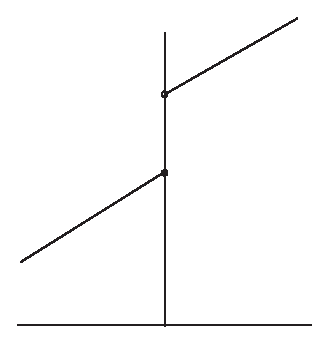
\includegraphics{PS/linear.eps}
  \caption{A piecewise linear function}
  \label{fig:discontinuous}
\end{figure}



We break the interval in two at $x=0$, forming two compact
intervals $[-1,0]$ and $[0,1]$.  We have continuous functions
$f_-:[-1,0]\to \R$ and $f_+:[0,1]$, such that
    $$
    f(x)=
    \begin{cases}
        f_-(x) & x\in[-1,0],\\
        f_+(x) & \text{otherwise}.
    \end{cases}
    $$
We have replaced the discontinuous function by a pair of
continuous functions on smaller intervals, at the expense of
duplicating the point of discontinuity $x=0$.  We view this pair
of functions as a single function $F$ on the compact topological
space with two components
    $$[-1,0]\times\{-\} \text{\ and\ } [0,1]\times\{+\}.$$
where $F(x,a) = f_a(x)$, and $a\in\{-,+\}$.

This is the approach that we follow in general with the Kepler
conjecture.  The function $\sigma$ is defined by a series of case
statements, and the function does not extend continuously across the
boundary of the cases.  However, in the degenerate cases that land
precisely between two or more cases, we form multiple copies of
decomposition star for each case, and place each case into a
separate compact domain on which the function $\sigma$ is
continuous.

This can be formalized as a {\it colored space}.  A colored space
is a topological space $X$ together with an equivalence relation
on $X$ with the property that no point $x$ is equivalent to any
other point in the same connected component as $x$.   We refer to
the connected components as colors, and call the points of $X$
{\it colored points}.  We call the set of equivalence classes of
$X$ the underlying uncolored space of $X$. Two colored points are
equal as uncolored points if they are equivalent under the
equivalence relation.
\index{colored!space}
\index{colored!points}

In our example, there are two colors ``$-$'' and ``$+$.''  The
equivalence class of $(x,a)$ is the set of pairs $(x,b)$ with the
same first coordinate.  Thus, if $x\ne0$, the equivalence class
contains one element $(x,\sign(x))$, and in the boundary case
$x=0$ there are two equivalent elements $(0,-)$ and $(0,+)$.

In our treatment of decomposition stars, there are various cases:
whether an edge has length less than or greater than $2t_0$, less
than or greater than $\sqrt8$, whether a face has circumradius
less than or greater than $\sqrt2$, and so forth. By duplicating
the degenerate cases (say an edge of exact length $2t_0$),
creating a separate connected component for each case, and
expressing the optimization problem on a colored space, we obtain
a continuous function $\sigma$ on a compact domain $X$.

The colorings have in general been suppressed in places from the
notation. To obtain consistent results, a statement about
$x\in[2,2t_0]$ should be interpreted as having an implicit
condition saying that $x$ has the coloring induced from the
coloring on the component containing $[2,2t_0]$.  A later
statement about $y\in[2t_0,\sqrt8]$ deals with $y$ of a different
color, and no relation between $x$ and $y$ of different colors is
assumed at the endpoint $2t_0$.




\shortversion{\chapter{Scoring~[Ferguson,~Hales]\index{Ferguson}}}
\longversion{\chapter{Scoring~[Ferguson,~Hales]\index{Ferguson}}}

\label{sec:scoring}

This \chap\  is coauthored by
Samuel P. Ferguson\index{Ferguson} and Thomas C. Hales.

In earlier \chaps, we describe each packing of unit balls by its set
$\Lambda\subset \ring{R}^3$ of centers of the packing.  We showed
that we may assume that our packings are saturated in the sense that
there is no room for additional balls to be inserted into the
packing without overlap. Lemma~\ref{lemma:deltabound} shows that the
Kepler conjecture follows if for each saturated packing $\Lambda$ we
can find a function $A:\Lambda\to\ring{R}$ with two properties: the
function is fcc-compatible and it is saturated in the sense of
Definition~\ref{def:negligible}.

The purpose of the first part of this \chap\ is to define a
function $A:\Lambda\to\ring{R}$ for every saturated packing
$\Lambda$ and to show that it is negligible.  The formula defining
$A$ consists of a term that is a correction between the volume of
the Voronoi cell $\Omega(v)$ and that of the $V$-cell $\op{VC}(v)$
and a further term coming from simplices of the $Q$-system that
have a vertex at $v$.

A major theorem in this \paper\ will be that this negligible
function is fcc-compatible.  The proof of fcc-compatibility can be
expressed as a difficult nonlinear optimization problem over the
compact topological space $\op{DS}$ that was introduced in
\Chap~\ref{sec:compact}.  In fact, we construct a continuous
function $A_0$ on the space $\op{DS}$ such that for each saturated
packing $\Lambda$ and each $v\in\Lambda$, the value of the function
$A$ at $v$ is a value in the range of the function $A_0$ on
$\op{DS}$. In this way, we are able to translate the
fcc-compatibility of $A$ into an extremal property of the function
$A_0$ on the space $\op{DS}$.

The proof of fcc-compatibility is more conveniently couched as an
optimization problem over a function that is related to the
function $A_0$ by an affine rescaling.   This new function is
called the score and is denoted $\sigma$.  (The exact relationship
between $A_0$ and $\sigma$ appears in Definition~\ref{def:score}.)
The function $\sigma$ is a continuous function on the space
$\op{DS}$. This function is defined in the final paragraphs of this
\chap.


\section{Definitions}
\label{sec:rules}


For every saturated packing $\Lambda$, and $v\in \Lambda$, there
is a canonically associated decomposition star $D(v,\Lambda)$. The
negligible function $A:\Lambda\to\ring{R}$ that we define is a
composite
  \begin{equation}
  A = A_0\circ D(\cdot,\Lambda)
  :\Lambda\to DS\to \ring{R},\quad v\mapsto D(v,\Lambda)\mapsto
  A_0(D(v,\Lambda)),
  \label{eqn:A}
  \end{equation}
where $A_0:\op{DS}\to\ring{R}$ is defined by
Equations~\ref{eqn:A1} and \ref{eqn:a1-sigma} below.  Each simplex
in the $Q$-system with a vertex at $v$ defines by translation to
the origin a simplex in the $Q$-system with a vertex at $0$
attached to $D(v,\Lambda)$. Let $\CalQ_0(D)$ be this set of
translated simplices at the origin. This set is determined by $D$.

\begin{definition} \label{def:context}
Let $Q$ be a quarter in $\CalQ_0(D)$.  We say that the {\it
context\/} of $Q$ is $\x(p,q)$ if there are $p$ anchors and $p-q$
quarters along the diagonal of $Q$. Write $c(Q,D)$ for the context
of $Q\in\CalQ_0(D)$.
\end{definition}\index{context (of a quarter)}

$q$ is the number of ``gaps'' between anchors around the diagonal.
For example, the context of a quarter in a quartered octahedron is
$\x(4,0)$.  The context of a single quarter is $\x(2,1)$.
%The
%only possible contexts of upright quarters in a quad cluster are
%$\x(4,0)$, $\x(3,1)$, and $\x(2,1)$. Of course, $Q$ and $\hat Q$
%have the same context. The definition of $\sigma(Q)$ depends on
%the context of $Q$.


The function $A_0$ will be defined to be
a continuous function on $\op{DS}$ of the
form
  \begin{equation}
  A_0(D) = -\op{vol}\,(\Omega(D)) + \op{vol}\,(\op{VC}(D)) +
   \sum_{Q\in\CalQ_0(D)} A_1(Q,c(Q,D),0).
   \label{eqn:A1}
   \end{equation}
Thus, the function $A_0$ measures the difference in volume between
the Voronoi cell and $V$-cell, as well as certain contributions
$A_1$ from the $Q$-system. The function $A_1(Q,c,v)$ depends on
$Q$, its context $c$, and a vertex $v$ of $Q$.  The function
$A_1(Q,c,v)$ will not depend on the second argument when $Q$ is a
quasi-regular tetrahedron.  (The context is not defined for such
simplices.)



\begin{definition} \label{def:rogers}
An {\it orthosimplex} consists of the convex hull of
$\{0,v_1,v_1+v_2,v_1+v_2+v_3\}$, where $v_2$ is a vector
orthogonal to $v_1$, and $v_3$ is orthogonal to both $v_1$ and
$v_2$.  We can specify an orthosimplex up to congruence by the
parameters $a = |v_1|$, $b=|v_1+v_2|$, and $c=|v_1+v_2+v_3|$,
where $a\le b\le c$. This parametrization of the orthosimplex
departs from the usual parametrization by the lengths $|v_1|$,
$|v_2|$, $|v_3|$. For $a\le b\le c$,  the {\it Rogers simplex\/}
$R(a,b,c)$ is an orthosimplex of the form
$$R(a,b,c)=S(a,b,c,\sqrt{c^2-b^2},\sqrt{c^2-a^2},\sqrt{b^2-a^2}).$$
See Figure~\ref{fig:rogers}.
%
 \index{Rogers simplex}
 \index{orthosimplex}
\end{definition}

\begin{figure}[htb]
  \centering
  \includegraphics{PS/rogers.eps}
  \caption{The Rogers simplex is an orthosimplex.}
  \label{fig:rogers}
\end{figure}

\begin{definition}\label{def:quoin}\index{quoin}
Let $R$ be a Rogers simplex.  We define the {\it quoin} of $R$ to
be the  wedge-like solid (a quoin) situated above $R$. It is
defined as the solid bounded by the four planes through the faces
of $R$ and a sphere of radius $c$ at the origin. (See
Figure~\ref{fig:quoin}.)   We let $\quo(R)$ be the volume of the
quoin over $R$.  \shortversion{An explicit formula appears in
\cite{KC}.}  \longversion{If $R=R(a,b,c)$ is a Rogers simplex, the
volume $\quo(R)$ is given explicitly as follows\index{Rogers
simplex}
    \begin{equation}
    \begin{array}{lll}
    6\quo(R) &= (a+2c)  %
    % -(a^2+ac-2c^2)
    (c-a)^2\arctan(e)
        +a(b^2-a^2)e\\&-4c^3\arctan(e(b-a)/(b+c)),
    \label{eqn:3.3}
    \end{array}
    \end{equation}
where $e\ge0$ is given by $e^2(b^2-a^2)=(c^2-b^2)$.}
%
 \index{quoin}
\end{definition}


\begin{figure}[htb]
  \centering
  \includegraphics{PS/quoin.eps}
  \caption{The quoin above a Rogers simplex is the part of the
  shaded solid outside
   the illustrated box.  It is bounded by the shaded planes, the plane through
   the front face of the box, and a sphere
   centered at the origin passing through the opposite corner of the box.}
  \label{fig:quoin}
\end{figure}

Let $S$ be a simplex and let $v$ be a vertex of that simplex. Let
$\op{VC}(S,v)$ be the subset of $|S|$ consisting of points closer
to $v$ than to any other vertex of $S$. By
Lemma~\ref{lemma:Q-divide}, if $S\in\CalQ_0(D)$, then
$$\op{VC}(S,0) = \op{VC}(D)\cap |S|.$$
Under the assumption that $S$ contains its circumcenter and that
every one of its faces contains its circumcenter, an explicit
formula for the volume $\op{vol}(\op{VC}(S,v))$ has been
calculated in \cite[Section~8.6.3]{part1}. This volume formula is
an algebraic function of the edge lengths of $S$, and may be
analytically continued to give a function of $S$ with chosen
vertex $v$:
  $$\op{vol}\,\op{VC}^\op{an}(S,v).$$

\begin{lemma}\label{lemma:cap-rogers}
Let $B(0,t)$ be a ball of radius $t$ centered at the origin.  Let
$v_1$ and $v_2$ be vertices.  Assume that $|v_1|< 2t$ and $|v_2|<2
t$.  Truncate the ball by cutting away the caps
   $$\op{cap}_i = \{x\in B(0,t) :  |x- v_i| < |x|\}.$$
Assume that the circumradius of the triangle $\{0,v_1,v_2\}$ is
less than $t$. Then the intersection of the caps $\op{cap}_1\cap
\op{cap}_2$ is the union of four quoins.
\end{lemma}

\begin{proof} This is true by inspection.  See Figure~\ref{fig:capriquoin}.
Slice the intersection $\op{cap}_1\cap\op{cap}_2$ into four pieces
by two perpendicular planes: the plane through $\{0,v_1,v_2\}$,
and the plane perpendicular to the first and passing through $0$
and the circumcenter of $\{0,v_1,v_2\}$.  Each of the four pieces
is a quoin.
\end{proof}

\begin{figure}[htb]
  \centering
  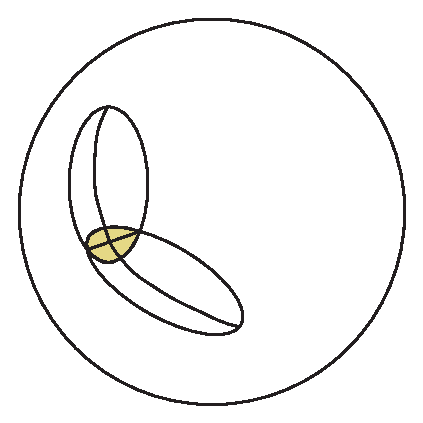
\includegraphics{PS/capriquoin.eps}
  \caption{The intersection of two caps on the unit ball can
   be partitioned into four quoins (shaded).}
  \label{fig:capriquoin}
\end{figure}

\begin{definition}\label{def:sol}
Let $v\in\ring{R}^3$ and let $X$ be a measurable subset of
$\ring{R}^3$. Let $\sol(X,v)$ be the area of the radial projection
of $X\setminus\{0\}$ to the unit sphere centered at the origin. We
call this area the {\it solid angle\/} of $X$ (at $v$).  When
$v=0$, we write the function as $\sol(X)$.
 %
 \index{sol}
 \index{solid angle}
\end{definition}


Let $S=\{v_0,v_1,v_2,v_3\}$ be a simplex. Fix $t$ in the range
$t_0\le t\le\sqrt2$.  Assume that $t$ is at most the circumradius
of $S$. Assume that it is at least the circumradius of each of the
faces of $S$.  Let $\op{VC}_t(S,v_0)$ be the intersection of
$\op{VC}(S,v_0)$ with the ball $B(v_0,t)$. Under the assumption
that $S$ contains its circumcenter and that every one of its faces
contains it circumcenter, an explicit formula for the volume
$$\op{vol}(\op{VC}_t(S,v_0))$$ is calculated by means of
Lemma~\ref{lemma:cap-rogers} through a process of inclusion and
exclusion. In detail, start with $|S|\cap B(v_0,t)$. Truncate this
solid by caps $\op{cap}_1$, $\op{cap}_2$,\index{cap} and
$\op{cap}_3$ bounded by the sphere of radius $t$ centered at $v_0$
and the perpendicular bisectors (respectively) of $\{v_0,v_1\}$,
$\{v_0,v_1\}$, $\{v_0,v_2\}$.  If we subtract the volume of each
cap $\op{cap}_i$, then we must add back the volume of the doubly
counted intersections of the caps.  The intersections of caps are
given as quoins (Lemma~\ref{lemma:cap-rogers}).  This leads to the
following formula. Let $h_i = |v_i|/2$ and
$\eta_{ij}=\eta(0,v_i,v_j)$, and let $S_3$ be the group of
permutations of $\{1,2,3\}$ in
\begin{equation}
   \op{vol}\,\op{VC}_t(S,v_0) =
   \sol(S)/3 - \sum_{i=1}^3 \frac{\dih(S,v_i)}{2\pi}\op{vol}\,\op{cap_i}
   +\sum_{(i,j,k)\in S_3} \quo(R(h_i,\eta_{ij},t)).
   \label{eqn:vol-theta-0}
\end{equation}


We extend Formula~\ref{eqn:vol-theta-0} by setting
    $$\quo(R(a,b,c)) = 0,$$
if the constraint $a < b < c$ fails to hold.  Similarly, set
$\op{vol}\,\op{cap}_i=0$ if $|v_i|\ge 2t$.  With these
conventions,  Formula~\ref{eqn:vol-theta-0} extends to all
simplices.  We write the extension of $\op{vol}\,\op{VC}_t(S,v)$
as
$$\op{vol}\,{\op{VC}^+_t}(S,v).$$



\begin{definition}\label{def:svor}
   Let\footnote{In the paper \cite{spp}, the volumes in this definition were
   volumes of Voronoi cells, and hence the notation $\vor$ for the function was
adopted. We retain $\vor$ in the notation, although this direct
connection with Voronoi cells has been lost.}
      $$
      \svor(S,v) = 4(-\doct \op{vol}\,\op{VC}^{\op{an}}(S,v)
         +\sol(S,v)/3),$$
      $$
      \svor(S,v,t) = 4(-\doct \op{vol}\,\op{VC}^+_{t}(S,v)
         +\sol(S,v)/3),$$
   and
      $$
      \svor_0(S,v) = \svor(S,v,t_0).
      $$
   When it is clear from the context that the vertex $v$ is
   fixed at the origin, we drop $v$ from the notation of these
   functions.
   If $S=\{v_1,v_2,v_3,v_4\}$, we define $\Gamma(S)$ as the average
   \begin{equation}
   \Gamma(S) = \frac{1}{4}\sum_{i=1}^4\svor(S,v_i).
   \label{eqn:gamma}
   \end{equation}
   The average $\Gamma(S)$ is called the {\it compression} of $S$.
%
 \index{compression}
 \index{ZZcamma@$\Gamma$}
\end{definition}

\begin{definition}
Let $Q$ be a quarter.   Let $\eta^+(Q)$ be the maximum of the
circumradii of the two faces of $Q$ along the diagonal of $Q$.
\end{definition}

Let $Q$ be a simplex in the $Q$-system.  We define an involution
$v\to \hat v$ on the vertices of $Q$ as follows.  If $Q$ is a
quarter and $v$ is an endpoint of the diagonal, then let $\hat v$
be the opposite endpoint of the diagonal.  In all other cases, set
$\hat v = v$.

We are ready to complete the definition of the function
$A:\Lambda\to\ring{R}$.  The definition of $A$ was reduced to that
of $A_0$ in Equation~\ref{eqn:A}.  The function $A_0$ was reduced
in turn to that of $A_1$ in Equation~\ref{eqn:A1}. To complete the
definition, we define $A_1$.

\begin{definition}\label{def:sigma}
Set
   \begin{equation}\label{eqn:a1-sigma}
   A_1(S,c,v) = -\op{vol}\,\op{VC}(S,v)+
      \frac{\sol(S,v)}{3\doct} - \frac{\sigma(S,c,v)}{4\doct}.
      \end{equation}  where $\sigma$ is given as follows:
      %
      \index{AZ1@$A_1$}
      \index{ZZsigma@$\sigma$}
\begin{enumerate}
\item If $S$ is a quasi-regular tetrahedron:
   \begin{enumerate}
      \item If the circumradius of $S$ less than $1.41$, set
         $$\sigma(S,-,v)=\Gamma(S)$$
      \item If the circumradius of $S$ is at least $1.41$, set
         $$\sigma(S,-,v)=\svor(S,v).$$
   \end{enumerate}
\item If $S$ is a strict quarter:
   \begin{enumerate}
      \item If $\eta^+(S) <\sqrt2$:
         \begin{enumerate}
         \item If the context $c$ is $(2,1)$ or $(4,0)$, set
                  $$\sigma(S,c,v)=\Gamma(S)$$
         \item If the context of $S$ is anything else, set
                  $$\sigma(S,c,v)=\Gamma(S) +
                     \frac{\svor_0(S,v)-\svor_0(S,\hat v)}{2}.$$
         \end{enumerate}
      \item If $\eta^+(S) \ge\sqrt2$:
         \begin{enumerate}
         \item If the context of $S$ is $(2,1)$, set
                  $$\sigma(S,c,v)=\svor(S,v).$$
         \item If the context of $S$ is $(4,0)$, set
                  $$\sigma(S,c,v)=\frac{\svor(S,v)+\svor(S,\hat v)}{2}.$$
         \item If the context of $S$ is anything else, set
                  $$\sigma(S,c,v)=\frac{\svor(S,v)+\svor(S,\hat
                  v)}{2}
                     +\frac{\svor_0(S,v)-\svor_0(S,\hat v)}{2}.$$
         \end{enumerate}
   \end{enumerate}
\end{enumerate}
When the context and vertex $v$ are given, we often write
$\sigma(S)$ or $\sigma(S,v)$ for $\sigma(S,c,v)$.

When $\eta^+<\sqrt2$, we say that the quarter has compression type.
Otherwise, we say it has Voronoi type.  To say that a quarter has
compression type means that $\Gamma(S)$ is one term of the function
$\sigma(S,v)$. It does not mean that $\Gamma(S)$ is equal to
$\sigma(S,v)$.
%
 \index{Voronoi type}
 \index{compression type}
\end{definition}

\longversion{The definition of $\sigma$ on quarters can be expressed
a second way in terms of a function $\mu$.  If $S$ is a quarter, set
    \begin{equation}
    \mu(S,v)=\begin{cases}
    \Gamma(S),&  \text{ if }\eta^+(S)<\sqr2,\\
    \svor(S,v),& \hbox{otherwise.}\end{cases}
    \label{eqn:3.8}
    \end{equation}
If $S$ is a flat quarter, we have $\sigma(S,c,v)=\mu(S,v)$, for all
contexts $c$.}

\longversion{Suppose $S$ is an upright
quarter.\index{quarter!upright} Definition~\ref{def:sigma} can be
expressed as follows.}

\longversion{
\begin{itemize}
 \item context $\x(2,1)$:  Set $\sigma(S,c,v)=\mu(S,v)$.
 \item context
    $\x(4,0)$:  Set $\sigma(S,c,v)=(\mu(S,v)+\mu(S,\hat v))/2$.
 \item other contexts:
 Set $\sigma(S,c,v)=(\mu(S,v)+\mu(S,\hat v)+ \svor_0(S,v) - \svor_0(S,\hat v))/2$.
\end{itemize}
 }


\begin{lemma}  $A_0:\op{DS}\to\ring{R}$ is continuous.
\end{lemma}

\begin{proof}
The continuity of $D\mapsto\op{vol}\,\op{VC}(D)$ is proved in
Lemma~\ref{lemma:vc-cont}.  The continuity of
$D\mapsto\op{vol}\,\Omega(D)$ is similarly proved.  The terms
$\op{vol}\,\op{VC}(S,v)$ and $\sol(S,v)$ are continuous. To complete
the proof we check that the function $\sigma(S,c,v)$ is continuous.
It is not continuous when viewed as a function of the set of
quarters, because of the various cases breaking at circumradius
$1.41$ and $\eta^+(S)=\sqrt2$.  However, these cutoffs have been
inserted into the data defining a decomposition star (in the
indexing sets $I_8$ and $I_9$).  Thus, the different cases in the
definition of $\sigma(S,c,v)$ land in different connected components
of the space $\op{DS}$ and continuity is obtained.
\end{proof}

We conclude this section with a result that will be of use in the
next section.

\begin{lemma}\label{lemma:A1-cancel}
Let $S=\{v_1,v_2,v_3,v_4\}$ be a simplex in the $S$-system,  and $c$
its context.   Then
   $$\sum_{i=1}^4 A_1(S,c,v_i)=0.$$
\end{lemma}

\begin{proof}
   By Formula~\ref{eqn:a1-sigma}, this is equivalent to
      \begin{equation}
      \sum_{i=1}^4 \sigma(S,c,v_i) = \sum_{i=1}^4
      \svor(S,c,v_i).
      \label{eqn:sigma-4}
      \end{equation}
Equation~\ref{eqn:sigma-4} is evident from
Definition~\ref{def:sigma} for $\sigma$.  In fact, the terms of the
form $\svor_0$ have opposing signs and cancel when we sum. The other
terms are weighted averages of the terms $\svor(S,c,v_i)$.
Equation~\ref{eqn:sigma-4} is thus established by noting that a sum
is unaffected by taking weighted averages of its terms.
\end{proof}


\section{Negligibility} \label{sec:negligible}

Let $B(x,r)$ be the closed ball of radius $r\in\ring{R}$ centered
at $x$.  Let $\Lambda(x,r)=\Lambda\cap B(x,r)$.

Recall from Definition~\ref{def:negligible} that a function
$A:\Lambda\to\ring{R}$ is said to be {\it negligible} if there is
a constant $C_1$ such that for all $r\ge1$, we have
   $$\sum_{v\in\Lambda(x,r) } A(v) \le C_1 r^2.$$
%
 \index{negligible}


Recall that a function $A: \Lambda\to\ring{R}$ given by
Equation~\ref{eqn:A}.  Explicitly, let
   $$A(v) = A_0(D(v,\Lambda)),$$
where $A_0$ in turn depends on functions $A_1$ and $\sigma$, as
determined by Equations~\ref{eqn:A1} and \ref{eqn:a1-sigma}, and
Definition~\ref{def:sigma}.

\begin{theorem}\label{lemma:negligible}
The function $A$ of Equation~\ref{eqn:A} is negligible.
\end{theorem}

\begin{proof} First we consider a simplification, where we replace
   $A$ with $A'$ defined by
      $$
      A'(v,\Lambda) = -\op{vol}(\Omega(D(v,\Lambda)))+
         \op{vol}(\op{VC}(D(v,\Lambda))).$$
(That is, at first we ignore the function $A_1$.) The Voronoi
cells partition $\ring{R}^3$, as do the $V$-cells.  We have
$\Omega(v,\Lambda)\subset B(v,2)$ (by saturation) and
$\op{VC}(v,\Lambda)\subset B(v,2\sqrt3)$ (by
Definition~\ref{def:phi}). Hence the Voronoi cells with $v\in
\Lambda(x,r)$ cover $B(x,r-2)$. Moreover, the $V$-cells with $v\in
\Lambda(x,r)$ are contained in $B(x,r+2\sqrt3)$.  Hence
   $$
   \sum_{v\in\Lambda(x,r)} A'(v) \le -\op{vol}\,B(x,r-2)
      +\op{vol}\,B(x,r+2\sqrt3)\le C_1' r^2
   $$
for some constant $C_1'$.

If we do not make the simplification, we must also include the sum
   $$\sum_{v\in\Lambda(x,r)} \sum_{Q\in\CalQ_v(D(v,\Lambda))}
      A_1 (Q,c,v).$$
Each quarter $Q=\{v_1,v_2,v_3,v_4\}$ in the $Q$-system occurs in
four sets $\CalQ_{v_i}(D(v_i,\Lambda))$.  By
Lemma~\ref{lemma:A1-cancel} the sum cancels, except when some
vertex of $Q$ lies inside $\Lambda(x,r)$ and another lies outside.
Each such simplex lies inside a shell of width $2\sqrt8$ around
the boundary.  The contribution of such boundary terms is again
bounded by a constant times $r^2$.  This completes the proof.
\end{proof}


\section{Fcc-compatibility}

We have constructed a negligible function $A$.  The rest of this
\paper\ will prove that this function is fcc-compatible.   This
section translates fcc-compatibility into a property that will be
easier to prove.  To begin with, we introduce a rescaled version
of the function $A$.

\begin{definition}\label{def:score}
Let $\sigma:\op{DS}\to\ring{R}$ be given by
   $$\sigma(D) = -4\doct (\op{vol}\,\Omega(D) + A_0(D)) +
   16\pi/3.$$
It is called the {\it score} of the decomposition star.
%
 \index{score}
 \index{ZZsigma@$\sigma(D)$}
\end{definition}

Recall from Definition~\ref{def:pt} the constant $\pt\approx
0.05537$.  This constant is called a point.\index{point}

\begin{lemma}\label{lemma:8pt-compat}
Let $A_0$, $A$, and $\sigma$ be the functions defined by
Equations~\ref{eqn:A}, \ref{eqn:A1}  \ref{eqn:a1-sigma}, and
Definition~\ref{def:sigma}. The following are equivalent.
\begin{enumerate}
  \item The minimum of the function on $\op{DS}$ given by
      $$D\mapsto \op{vol}\,\Omega(D) + A_0(D)$$
is $\sqrt{32}$.
  \item The maximum of $\sigma$ on $\op{DS}$ is $8\,\pt$.
\end{enumerate}
Moreover, these statements imply
\begin{itemize}
  \item For every saturated packing $\Lambda$,
  the function $A$ is
  fcc-compatible.
\end{itemize}
\end{lemma}

(Eventually, we prove fcc-compatibility by proving
$\sigma(D)\le8\,\pt$ for all $D\in\op{DS}$.)

\begin{proof} To see the equivalence of the first and second statements,
use Definition~\ref{def:score},  and the identity
   $$8\,\pt = -4\doct (\sqrt{32}) + 16 \pi/3.$$
(Note that this identity is parallel in form with
Definition~\ref{def:score} for $\sigma$.)

For a given saturated packing $\Lambda$, the function $A$ has the
form $A(v) = A_0(D(v,\Lambda))$.  Also, $\Omega(D(v,\Lambda))$ is
a translate of $\Omega(v)$, the Voronoi cell at $v$.  In
particular, they have the same volume.  Thus,
$\op{vol}\,\Omega(v)+A(v)$ lies in the range of the function
   $$\op{vol}\,\Omega(D) + A_0(D)$$
on $\op{DS}$.  The minimum of this function is $\sqrt{32}$ by the
first of the equivalent statements.  It now follows from the
definition of fcc-compatibility, that $A:\Lambda\to\ring{R}$ is
indeed fcc-compatible.
\end{proof}

\begin{theorem}\label{lemma:exista}
If the maximum of the function $\sigma$ on
$\op{DS}$ is $8\,\pt$, then for every saturated packing $\Lambda$
there exists a negligible fcc-compatible function $A$.
\end{theorem}

\begin{proof} This follows immediately from Theorem~\ref{lemma:negligible}
and Lemma~\ref{lemma:8pt-compat}.
\end{proof}



\section{Scores of Standard Clusters}
\label{sec:ssc}

The last section introduced a function $\sigma$ called the score. We
show that the function $\sigma$ can be expressed as a sum over terms
attached to each of the standard regions.

\begin{definition} \label{def:standard-cluster}
A {\it standard cluster\/} is a pair $(R,D)$ where $D$ is a
decomposition star and $R$ is one of its standard regions.  A {\it
quad cluster\/} is the standard cluster obtained when the standard
region is a quadrilateral.
\end{definition}
%
 \index{cluster!standard}
 \index{cluster!quad}
 \index{quad cluster}

%Recall $|S|$ is the convex hull of a set $S\subset
%\ring{R}^3$.

We break $\sigma$ into a sum
   \begin{equation}
   \sigma(D) = \sum_R\,\sigma_R(D),
   \end{equation}
indexed by the standard clusters $(R,D)$.  Let
   $$
   \op{VC}_R(D) = \op{VC}(D)\cap \op{cone}(R),
   $$
whenever $R$ is a measurable subset of the unit sphere.  Let
   $$
   \CalQ_0(R,D) = \{Q\in \CalQ_0(D) : Q\subset \op{cone}(R)\}.
   $$
By Lemma~\ref{lemma:Q-in-region},
 each $Q$ is entirely contained in the cone over a single
standard region.

\begin{definition} \label{def:score-std-region}
   Let $R$ be a measurable subset of the unit sphere.  Set
      $$
      \vor_R(D) =4\left(-\doct \op{vol}\,\op{VC}_R(D)  + \sol(R)/3\right)
      $$
      Let $R$ be a standard region. Set
      $$
      \sigma_R(D) = \vor_R(D) - 4\doct
         \sum_{Q\in\CalQ_0(R,D)} A_1(Q,c(Q,D),0).
      $$
\index{vzorR@$\vor_R$} \index{zzsigmaR@$\sigma_R$}
\end{definition}

\begin{lemma} $\sigma(D) = \sum_R\sigma_R(D)$, where the sum runs
over all standard regions $R$.
\end{lemma}

\begin{proof}
   $$
   \begin{array}{lll}
      \sigma(D)
      &= -4\doct (\op{vol}\,\Omega(D) + A_0(D))+16\pi/3\\
      &= -4\doct (\op{vol}\,\op{VC}(D)+\sum_{Q\in\CalQ_0(D)}
         A_1(Q,c(Q,D),0)) + (4) (4\pi/3)\\
      &= \sum_R 4\left (-\doct \op{vol}\,\op{VC}_R(D) -\doct
         \sum_{Q\in\CalQ_0(R,D)} A_1(Q,c(Q,D),0) +
         \sol(R)/3\right).
   \end{array}
   $$
\end{proof}

\longversion{
Also, we have
    \begin{equation}
    \op{vor}(D)=\sum_{R\in \CalR(D)}
    \op{vor}_R(D).
    \label{eqn:vorD}
    \end{equation}
    }

\begin{lemma}\label{lemma:R'}
Let $R'\subset R$ be the part of a standard region that does not
lie in any cone over any $Q\in Q_0(R,D)$.  Then
   $$
   \sigma_R(D) = \vor_{R'}(D)
      + \sum_{Q\in\CalQ_0(R,D)} \sigma(Q,c(Q,D),0).
   $$
\end{lemma}

\begin{proof} Substitute the definition of $A_1$
(Equation~\ref{eqn:a1-sigma}) into the definition of
$\sigma_R(D)$, noting that $\op{VC}(Q,0) = \op{VC}_{R''}(D)$,
where $R''$ is the intersection of $Q$ with the unit sphere.
\end{proof}

\begin{remark}   Lemma~\ref{lemma:R'} explains why we have chosen
the same symbol $\sigma$ for the functions $\sigma_R(D)$ and
$\sigma(Q,c,v)$.  We can view Lemma~\ref{lemma:R'} as asserting a
linear relation in the functions $\sigma$:
   $$\sigma_R(D) = \sigma_{R'}(D) + \sum \sigma(Q,c,0).$$
The sum runs over $Q\in\CalQ_0$ that lie in the cone over $R$.
\end{remark}

\longversion{\section{Scores of Simplices and Cones}}

\longversion{Many of the functions in this paper are defined by
terms involving volumes of simple solids.  To give estimates on the
functions, it is often convenient to partition the solids into
smaller pieces and then define corresponding functions on each of
the pieces.  For this reason, we define some variants of the
functions $\vor$ and $\sigma$.}

\longversion{
\begin{remark}\label{remark:vor}\index{vor}\index{c-vor}\index{score}
We now define a few more variants of the function $\vor$. The
function $\svor$ and its truncated version  $\svor(\cdot,t)$ have
been defined already. The function $\vor_R(D)$ will also be given a
truncated version $\vor_R(D,t)$, for a real truncation parameter
$t\ge 0$. The special case, $\vor_R(D,t_0)$ will be abbreviated
$\vor_{0,R}(D)$. There will be another variant $\op{r-vor}$ for
Rogers simplices, and another $\op{c-vor}$ for general sets.  The
general form of these functions is
    $$\op{c-vor}(X) = 4 (-\doct\op{vol}(X) + \sol(X)/3),$$
for any subset $X\subset \ring{R}^3$.   The differences between the
different versions of $\vor$ come from the different choices of the
set $X$ and the way they are parameterized.
\end{remark}}

\longversion{
\begin{definition}  \label{def:r-vor}\index{r-vor}
Let $R=R(a,b,c)$ be a Rogers simplex. Assume that the
vertex terminating the edges of lengths $a$, $b$, and $c$ is
situated at the origin. Let
    $$\op{r-vor}(R) = 4 (-\doct\op{vol}(R) + \sol(R)/3).$$
\end{definition}}


% \index{Voronoi function} We define the simplex
%version $\svor$ of the function as follows. We begin with its
%definition for simplices $S$ whose faces have positive
%orientation. Assume that $S$ has a distinguished vertex $v$, which
%e fix at the origin. Let $\sol(S)$ be the solid angle of $S$ at
%its distinguished vertex.\index{sol} Set
%$\doct=(\pi-4\arctan(\sqr2/5))/\sqr8$. Set
%    \begin{equation}
%   \svor(S) = 4(-\doct \op{vol}(\op{VC}(S,0)) + \sol(S)/3),
%   \label{eqn:3.1}
%    \end{equation}
%This formula may be analytically continued to simplices $S$ with
%negatively oriented faces, and $\svor(S)$ is defined in general by
%this analytic continuation. A formula for $\svor$ is found in
%\cite[Sec. 8.6]{part1}.  Let $S_1,\ldots, S_4$ be equal to $S$
%as unlabeled simplices, but with different distinguished vertices.

\longversion{
\begin{definition}\label{def:cone}
 Let $C(h,t)$ denote the compact cone of height $h$
and circular base. Set
%of area $\pi(t^2-h^2)$. Set
    $$
    \phi(h,t)=2(2-\doct  t h (h+t))/3.
    $$
\index{right circular cone}\index{cone}
 Then
    \begin{equation}
    \op{c-vor}(C(h,t))=2\pi(1-h/t)\phi(h,t).
    \label{eqn:3.2}
    \end{equation}
 \end{definition}
    }

\longversion{
\begin{remark}\label{remark:score}
Below, we introduce variants of the function $\sigma$. We have
already encountered $\sigma$ in Definitions~\ref{def:sigma},
\ref{def:score}, and \ref{def:score-std-region}. Informally, we call
$\sigma$ (and various functions that are closely related to it) the
{\it score}. Equation~\ref{eqn:3.2} represents the {\it score\/} of
$C(h,t)$. The solid angle of $C(h,t)$ is $2\pi(1-h/t)$, so
$\phi(h,t)$ is the score per unit area. Also, $\phi(t,t)$ is the
score per unit area of a ball of radius $t$. That is, $\phi(t,t) =
4(-\doct\op{vol}/\sol + 1/3)$.\index{score}
\end{remark}
}


\longversion{ We set
    \begin{equation}
    \begin{array}{lll}
    \svor(S,t) &=
    \sol(S)\phi(t,t)
    +\sum_{i=1,\ h_i\le t}^3 d_i (1-h_i/t) (\phi(h_i,t)-
    \phi(t,t)) \\
    &-\sum_{(i,j,k)\in S_3}
    4\doct
    \quo(R(h_i,\eta(y_i,y_j,y_{k+3}),t)).
    \label{eqn:3.5}
    \end{array}
    \end{equation}
In the definition, we adopt the convention that $\quo(R)=0$, if
$R=R(a,b,c)$ does not exist (that is, if the condition
    $0< a\le b\le c$
is violated). In the second sum, $S_3$ is the set of permutations on
three letters. This definition is compatible with
Definition~\ref{def:svor}.}


%This formula has a simple geometric interpretation when the
%circumradius of $S$ is greater than $t$ and the circumradius of
%each face is less than $t$. It represents the score\index{score}
%of the part of the Voronoi cell at the origin that lies inside $S$
%and inside a ball of radius $t$.  This can be seen geometrically
%from Figure~\ref{fig:diag36}, which depicts the intersection of
%$S$ with the Voronoi cell as three quadrilaterals forming a
%triangle. The truncation in the second frame is shown as a shaded
%region. The truncated volume can be decomposed into a solid angle
%term, three conic terms, and six quoins (with appropriate sign
%conventions).  Hence the formula for $\svor(S,t)$. }



\longversion{ Similarly, we define $\vor_P(D,t)$ for arbitrary
standard clusters $(P,D)$.  (We shift notation from $R$ to $P$ for a
standard region to avoid conflict with Rogers simplices $R$ in the
following definition.)  Extending the notation in an obvious way, we
have
    \begin{equation}
    \begin{array}{lll}
    \vor_P(D,t) &=
    \sol(P)\phi(t,t)
    +\sum_{|v_i|\le 2t} d_i (1-|v_i|/(2t)) (\phi(|v_i|/2,t)-
    \phi(t,t)) \\
    &-\sum_{R} 4\doct \quo(R).
    \label{eqn:3.7}
    \end{array}
    \end{equation}
The first sum runs over vertices in $P$ of height at most $2t$. The
second sum runs over Rogers simplices $R(|v_i|/2,\eta(F),t)$ in $P$,
where $F=\{0,v_1,v_2\}$ is a face of circumradius $\eta(F)$ at most
$t$, formed by vertices in $P$.  The constant $d_i$ is the total
dihedral angle along $\{0,v_i\}$ of the standard cluster. The
truncations $t=t_0=1.255$ and $t=\sqr2$ will be of particular
importance.
    Set $A(h) = (1-h/t_0) (\phi(h,t_0)-\phi(t_0,t_0))$.\index{A}}

\longversion{
\begin{remark}  We have introduced both untruncated and truncated
versions of functions $\vor$ and $\sigma$.  The truncated versions
are used to give upper bounds on the untruncated versions.  For
example,  in the function $\sigma(D)$, the $V$-cell contributes
through its volume, as in Remark~\ref{remark:vor}.  The volume
appears with a negative coefficient $-4\doct$.  Thus, we obtain an
upper bound on $\sigma(D)$ by discarding bits of volume from the
$V$-cell.   This suggests that we might try to give upper bounds on
the score $\sigma(D)$ by truncating the $V$-cell in various ways.
This is the reason for the truncated versions of these functions.
\end{remark}}

\longversion{\section{The Example of a Dodecahedron}}

\longversion{
\begin{example}  The following example illustrates why better bounds
on the density of packings can be obtained with $\sigma(D)$ than
with a naive approach based on the volume of Voronoi cells.  By
scoring quasi-regular tetrahedra with the compression function
$\Gamma(S)$ rather than $\op{s-vor}(S)$, we will find that the score
is lowered below $8\,\pt$ for configurations with many quasi-regular
tetrahedra. To work one example, let us assume that the
decomposition star consists of $12$ vertices located at distance $2$
from the origin, at the vertices of a regular icosahedron. The score
is approximately
   $$20\,\Gamma(S(2,2,2,2.1092,2.1092,2.1092) \approx 1.8\,\pt < 8\,\pt.$$
If $\op{s-vor}(S)$ had been used, the score would violate Theorem
1.7:
   $$20\,\op{s-vor}(S) \approx 13.5493\,\pt > 8\,\pt.$$
(This is tied to the fact that the regular dodecahedron of
inradius $1$ has smaller volume than the rhombic dodecahedron of
inradius $1$.)
\end{example}
}

    % Flyspeck
% Thomas C. Hales
% Starting with Chapter on Tame Hypermaps

% Sep 3, Removed 2 enclosed in quad properties.

\chapter{Tame Hypermap}
\indy{Index}{hypermap!tame}%

\label{sec:tame}
\indy{Index}{tame}%

\begin{summary}
This chapter is the second of the two core chapters that are devoted to the proof of the Kepler Conjecture.  If $V$ is a finite set of vectors in $\ring{R}^3$, let
$$\CalL(V) = \sum_{v\in V} L(\normo{v}/2).$$
Let $\bar B(0,r)$ be the closed ball of radius $r$.
By Corollary~\ref{cor:CE}, it suffices to show that every finite packing $V$
contained in $\bar B(0,2h_0)\setminus B(0,2)$
satisfies
\begin{equation}\label{eqn:CCE}
\CalL(V) \le 12.
\end{equation}

This chapter assumes that there exists a counterexample $V$ to this inequality and reaches a contradiction.  A subset of extremal counterexamples will be selected that are particularly well-suited for further analysis.  Every extremal counterexample gives rise to a fan and a corresponding hypermap.  
A detailed study of these hypermaps leads to a long list of properties that all such hypermaps must
possess.   A {\it tame} hypermap is defined to be precisely the set of hypermaps that have all of these
properties.   Tameness is thus an umbrella term that covers a long list of loosely related properties.

An earlier chapter on hypermaps gives an algorithm that generates all restricted hypermaps (with a given bound on the number of nodes).   Every tame hypermap is restricted and has at most $14$ nodes.  Hence a list of all tame hypermaps can be obtained by generating all restricted hypermaps and filtering out those that are not tame.   This algorithm has been implemented in computer code and run.  The result is that there is an explicit complete list of all tame hypermaps (up to isomorphism).  
This list gives the classification of tame hypermaps up to isomorphism.   This classification solves a
major step of the packing problem.

Each tame hypermap $H$ gives rise to a nonlinear optimization problem.   Maximize $\CalL(V)$ subject to the constraint that the hypermap associated with  $V$ 
is isomorphic to $H$.  This nonlinear optimization problem has a linear relaxation.  This linear program has
a maximum that is at least as large as the maximum of the nonlinear program.  The linear programs
have been solved by computer.  In every case, the maximum is less than $12$.  This means
that inequality~\ref{eqn:CCE} always holds, so that the Kepler Conjecture is confirmed.
\end{summary}
\indy{Index}{hypermap!tame}%
\indy{Index}{tame!hypermap}%



\section{Definition}


\begin{definition}[triangle,~quadrilateral]
Faces of cardinality $3$ in a hypermap are called {\it triangles}, those of
cardinality $4$ are called {\it quadrilaterals}, and so forth.  
 %
 \indy{Index}{triangle}%
 \indy{Index}{quadrilateral}%
 \indy{Notation}{pZ@$p_v$}%
\end{definition}

\begin{definition}[type,~$(p,q,r)$]\label{definition:type}
The {\it type\/} of a node is defined to be a triple of
non-negative integers $(p,q,r)$, where $p$ is the number of
triangles meeting the node, $q$ is the number of quadrilaterals
meeting it, and $r$ is the number of other faces meeting it, so that
$p+q+r$ is the total number of faces meeting the node.
%
 \indy{Index}{node!type}%
\indy{Notation}{pqr@$(p,q,r)$}%
\end{definition}


\subsection{weight assignment}\label{sec:wtassign}
\indy{Index}{weight assignment}%

Call the constant $\op{tgt}=1.541$, which arises repeatedly in
this chapter, the {\it target}. 
%
 \indy{Index}{target}%
\indy{Notation}{tgt@$\op{tgt}=1.541$}%


\begin{definition}[b]
  Define $b:\ring{N}\times \ring{N}\to \ring{R}$ by $b(p,q)=\op{tgt}$,
  except for the values in the following table:
  {
  \def\tx{\op{tgt}}
  $$\begin{matrix}  &q=0&1&2&3&4\\
           p=0&\tx&\tx&\tx&0.618&1.0\\
           1&\tx&\tx&0.66&0.618&\tx\\
           2&\tx&0.8&0.412&1.2851&\tx\\
           3&\tx&0.315&0.83&\tx&\tx\\
           4&0.35&0.374&\tx&\tx&\tx\\
           5&0.04&1.144&\tx&\tx&\tx\\
           6&0.689&\tx&\tx&\tx&\tx\\
           7&1.450&\tx&\tx&\tx&\tx
   \end{matrix}
   $$
   }
\indy{Notation}{b@$b$ (tame)}%
\end{definition}


\begin{definition}[d]
    Define $d:\ring{N}\to \ring{R}$ by
  $$d(k) = \begin{cases}
    0 & k\le3, \\
    0.206 & k=4, \\
    0.4819 & k=5, \\
    0.7578 & k=6, \\
    %1.038 & k=7, \\
    %1.315 & k=8,\\
    \op{tgt}=1.541 & \text{otherwise}.
  \end{cases}
  $$
\indy{Notation}{d@$d$ (tame)}%
\end{definition}




\begin{definition}[weight~assignment]
%
A {\it weight assignment\/} of a hypermap $H$ is a function $\tau$ on
the set of faces of $H$, taking values in the set of non-negative
real numbers. A weight assignment is {\it admissible} if the
following properties hold:
%
 \indy{Index}{weight assignment}%
 \indy{Index}{weight assignment!admissible}%
 \indy{Index}{cardinality}%
 \indy{Index}{node}%
 \indy{Notation}{ZZtau@$\tau$ (weight assignment)}%
\begin{nomerate}
 \item \case{bound~a} Let $v$ be any node of type $(5,0,1)$, and let $A$ be the set of
triangles meeting that node.
        Then
        $$\sum_{F\in A} \tau(F)
            \ge  0.63.$$
%   where $a=0.63$.
%        \label{definition:admissible:excess}
 \item \case{bound~b} If a node $v$ has type $(p,q,0)$, then
        $$\sum_{F:\,v\cap F\ne\emptyset} \tau(F) \ge b(p,q).$$
%        \label{admissible:b}
  \item \case{bound~d} If the face $F$ has cardinality $k$, then
        $\tau(F) \ge d(k)$.
\end{nomerate}
\indy{Notation}{v@$v$ (node)}%
\indy{Notation}{A@$A$ (set of triangles)}%

The sum $\sum_F \tau(F)$ (over all faces) is called the {\it total weight}. % of $\tau$.
\indy{Index}{weight!total}%
%\indy{Notation}{total@$\sum\tau$}%
\end{definition}





\subsection{hypermap property}
\label{sec:graphproperty}

A hypermap is {\it tame\/} if it satisfies the following conditions.
%
 \indy{Index}{tame}%

\begin{itemize}
    \label{definition:tame}
    %1
    \item \case{planar}  The hypermap is plain and planar.
    \item \case{simple} The hypermap is connected and simple.  In particular, every intersection of a face with a node contains at most one dart.
    \item \case{nondegenerate} The edge map $e$ has no fixed points.
    \item \case{no loops} The two darts of each edge lie in different nodes.
    \item \case{no double joins} At most one edge meets any two given nodes.
%    \label{definition:tame:40}
%    \item \case{blank}
\indy{Notation}{edgemapz@$e$ (edge map)}%
%    \item \case{triangles} If $L$ is a contour loop with three face steps, and if there exists a node in
%    the exterior of $L$, then $L$ is a face of the hypermap.
%    \label{definition:tame:3-circuit}
%\item \case{blank}
 %   \item \case{quadrilaterals} If $L$ is a contour loop with four face steps, and there are at least two nodes    in the exterior of $L$, then the interior of $L$ takes one of the forms     illustrated in Figure
 %   \ref{fig:fourcircuit}.
 %   \label{definition:tame:4-circuit}
  %  \begin{figure}[htb]
  %      \centering
  %      \myincludegraphics{\pdfp/fourcircuit.eps}
  %      \caption{Tame $4$-circuits}
  %      \label{fig:fourcircuit}
  %  \end{figure}
  \item \case{face count} The hypermap has at least three faces.
    \item \case{face size} The cardinality of each face is at least $3$ and at most $6$.
    \item \case{node count} There are either $13$ or $14$ nodes.
    \item \case{node size} The cardinality of every node is at least $3$ and at most
    $7$.
  %    \label{definition:tame:degree}
    \item \case{node types} If a node has cardinality $7$, then the type of the
       node is $(p,q,0)$ for some $p,q\ge0$.   If the
        cardinality of the node is exactly $6$, then the type of the node
        is $(5,0,1)$.
%    \label{definition:tame:degreeE}
    \item \case{weights} There exists an admissible weight assignment
        of total weight less than the target, $\op{tgt}=1.541$.
\end{itemize}
%
\indy{Index}{planar}%
\indy{Index}{simple}%
\indy{Index}{nondegenerate}%
\indy{Index}{no loops}%
\indy{Index}{no double joins}%
\indy{Index}{face}%
\indy{Index}{weight}%

\section{Classification}
    \label{sec:proof-classification}

%\section{Statement of the Theorem}
\label{sec:classification}




\begin{definition}[opposite] The opposite of a hypermap $(D,e,n,f)$ is the
hypermap $(D,f n,n^{-1},f^{-1})$.
\indy{Index}{hypermap!opposite}%
\end{definition}

\begin{lemma}\guid{PPHEUFG}
\oldrating{300}
\rating{0}
\formalauthor{Diep Trieu Thi} 
A hypermap is tame if and only if its opposite hypermap is tame as well.
\end{lemma}

A list of hypermaps appears at \cite{website:Hales:1998:Code}.

\begin{theorem}\guid{WTEMDTA}
\label{theorem:classification} Every tame hypermap is isomorphic to
a hypermap in the list~\cite{website:Hales:1998:Code}, or is isomorphic to the opposite of a
hypermap in the list.
\indy{Index}{isomorphic}%
\end{theorem}

\begin{note}%XX
The (java version of the) graph generator has been run with the new parameters described in this version of the book.  It produces finitely many graphs (about 25,000).  This new list will eventually replace the archive from 1998.  The Bauer-Nipkow formalization of the classification has not yet been adapted to this new definition of tameness.
\indy{Index}{Java}%
\end{note}


Computers are used to generate a list of all hypermaps and to check
them against the archive of tame hypermaps.  The computer program is
based on the hypermap generation construction of Section~\ref{sec:face-insert}.  According
to the results of that section, every restricted hypermap can be generated by an
elementary edge-insertion algorithm.  Every tame hypermap is a restricted hypermap.
The list of restricted hypermaps can be filtered to obtain a complete list of tame hypermaps.
\indy{Index}{computer calculation}%

\section{Contravening hypermap}

\indy{Index}{hypermap!contravening}%
%The aim is to prove Conjecture~\ref{conj:L12}.  For a contradiction, assume a counterexample. 
A counterexample to the Kepler conjecture leads to a finite packing $V\subset \bar B(0,2h_0)\setminus B(0,2)$ that violates the inequality~(\ref{eqn:CCE}).
 The purpose of this section is to select a special class of counterexamples to this inequality.
Let
\begin{equation}\label{eqn:fan-edge}
\begin{array}{lll}
 E_{std} &= \{\{v,w\}\in V^2\mid 0 < \norm{v}{w}\le 2\hm \}\\
 E_{ctc} &= \{\{v,w\}\in V^2\mid \norm{v}{w}= 2 \}\subset E_{std}.
\end{array}
\end{equation}

\begin{lemma}\guid{UBHDEUU}\rating{140}
$(V,E)$ is a fan, if $E=E_{std}$ or $E=E_{ctc}$.
\end{lemma}
$(V,E_{std})$ and $(V,E_{ctc})$ are called the standard fan and contact fan, respectively.
Let $\op{hyp}(V,E)$ be the associated hypermap.
\indy{Index}{fan!standard}%
\indy{Index}{fan!contact}%
\indy{Notation}{V@$V$ (packing)}%
\indy{Notation}{V@$( V, E ) $ (fan)}%
\indy{Notation}{hyp@$\op{hyp}$ (hypermap)}%
\indy{Notation}{E@$E_{std}$}%
\indy{Notation}{E@$E_{ctc}$}%

\begin{definition}[isolated,~surrounded]
Let $(V,E)$ be a fan.
Say that $v\in V$ is {\it isolated} in the fan if $E(v)$ is empty.
(That is, the degree of the corresponding node in the hypermap is $0$.) Say that $v\in V$ is {\it surrounded} in the fan if the azimuth angles of all darts at the node $v$ are less than $\pi$.  (In particular, the cardinality of $E(v)$ is at least three.)
\end{definition}
\indy{Index}{isolated}%
\indy{Index}{surrounded}%
\indy{Index}{angle!azimuth}%
\indy{Index}{azimuth}%
\indy{Index}{cardinality}%
\indy{Notation}{E@$E(v)$ (fan)}%

The following lemma appears in Sch\"utte and van der Waerden~\cite{vanderWaerden:1951}.

\begin{lemma}\guid{FATUGPD}\rating{200}
Given any packing $V\subset \bar B(0,2\hm)\setminus B(0,2)$,
there exists a  packing $V'$ 
in bijective correspondence with $V$:
$$
\phi:V\to V'
$$
such that $\normo{v} = \normo{\phi(v)}$ and
such that every vertex $v'$ in the contact fan of $V'$
is either isolated or surrounded.
\end{lemma}
\indy{Index}{packing!finite}%
\indy{Index}{fan!contact}%
\indy{Notation}{V@$V'$ (packing)}%

\begin{proof} Consider all finite packings in 
bijective correspondence with $V$, such that the
bijection preserves distances of points from the origin.
Among these packings, pick one $V'$ with the largest number
of isolated points in the contact graph.  If there is a point $v\in V'$ that
is not isolated and not surrounded, then it has a contact
dart with angle at least $\pi$.   Perturb $v$ away from the contacts, making it isolated, while preserving its distance to $\orz$.  The perturbed packing $V''$ has one more isolated point than $V'$, which is contrary to the supposed maximality of $V'$.  Hence, the conclusion of the 
lemma holds for $V'$.
\end{proof}

The following lemma shows that the corresponding result
holds for the standard fan.  Reader beware!  The set of isolated and surrounded vertices depends on a 
choice of fan.  The next proof makes heavy use of two different fans $(V,E_{std})$ and $(V,E_{ctc})$,
which have different sets of isolated and surrounded vertices, even though the set $V$ is
the same in both cases.



\begin{lemma}\guid{FJLBXS}\rating{1000}\label{lemma:surrounded}  % was rating{500}.
Given any packing $V\subset \bar B(0,2\hm)\setminus B(0,2)$,
there exists a  packing $V'$ 
in bijective correspondence with $V$:
$$
\phi:V\to V'
$$
such that $\normo{v} = \normo{\phi(v)}$ and
such that every vertex $v'$ in the standard fan of $V'$
is isolated or surrounded.
\indy{Index}{packing!finite}%
\end{lemma}

\begin{proof}  For any packing $V'\subset \bar B(0,2\hm)\setminus B(0,2)$, let $V'_{iso},V'_{sur}$ be the
sets of isolated and surrounded vertices of $V'$ respectively, in the {\bf contact}
fan.  
By the previous lemma,  assume
without generality that every vertex $v$ in the contact fan of $V$ is either isolated
or surrounded:
$$
V = V_{iso} \cup V_{sur}.
$$
Consider the set $\CalV$ of pairs $(V',\phi)$ consisting of a packing $V'$
and bijection $\phi:V\to V'$ such that
\begin{itemize}
\item $\phi$ preserves distances from the origin, 
\item $V_{sur}=V'_{sur}$, and 
\item the restriction of $\phi$ to $V_{sur}$ is the identity map $I$.
\end{itemize}
\indy{Notation}{V@$\CalV$ (family of packings)}%%
\indy{Notation}{V@$V_{iso}$ (contact isolated vertices)}%%
\indy{Notation}{V@$V_{sur}$ (contact surrounded vertices)}%%
\indy{Notation}{I@$I$ (identity map)}%

\claim{The set $\CalV$ is a nonempty compact topological space.}  Indeed, by fixing an enumeration
$V = \{v_0,\ldots,v_r\}$,  
the set $\CalV$ embeds into Euclidean space of dimension $3r$ under the map that sends
the pair $(V',\phi)$ to 
the point $(\phi^{-1}v_0,\ldots,\phi^{-1}v_r)$.
Thus, $\CalV$ carries a metric space topology as a subset of Euclidean space.  With a little
argument, it follows from the boundedness of $V\subset B(0,2\hm)$ that $\CalV$ is compact.
Also, $(V,I)\in \CalV$, so $\CalV\ne\emptyset$.


For any pair $(V',\phi)$ in $\CalV$ and $w\in \phi(V_{iso})$, let
$c(V',\phi,w)$, 
be the minimum distance of $w$ to a point
in $V'\setminus \{w\}$.   
For $i=1,\ldots,n=\card(V_{iso})$
define constants $c_i=c_i(V',\phi)$,
by ordering the real numbers $c(V',\phi,w)$, $w\in\phi(V_{iso})$, in increasing order:
$$
c_0 \le c_1 \le c_2 \le \cdots \le c_n.
$$
The constants $c_i:\CalV\to\ring{R}$ are continuous functions on the compact configuration space $\CalV$.
There is a nonempty 
compact subset $\CalV_0$ of $\CalV$ on which
$c_0$ attains its maximum value. Continuing recursively,
there is a nonempty compact subset $\CalV_{i+1}$ of
$\CalV_{i}$ on which $c_i$ attains its maximum value.
\indy{Notation}{c i@$c_i$ (constant)}%
\indy{Notation}{V@$\CalV_0$}%

For the configuration $(V,I)\in \CalV$, it follows that $c_0(V,I) >2$.
Hence, $c_0(V',\phi)>2$ for $(V',\phi)\in\CalV_0$.  It follows
that $V'_{iso}$ is in bijective correspondence with
$V_{iso}$, for all $(V',\phi)\in \CalV$.

\claim{Any $(V',\phi)\in \CalV_n$ has the desired property.} Otherwise,
there exists some vertex $v'\in V'_{iso}$ (in contact isolation)
is neither isolated nor surrounded in the standard fan.  
Any such vertex satisfies $c(V',\phi,\phi(v'))=c_i(V',\phi)$ for some $i$.
Among such vertices, pick the vertex with smallest index
$i$.  Write 
$$
c(V',\phi,\phi(v')) = c_i(V',\phi) = c_{i+1}(V',\phi) =\cdots= c_j(V',\phi) < c_{j+1}(V',\phi),
$$
for some $j\ge i$.  As $v'$ is not isolated in the
standard fan, it follows that $c_j(v') < 2\hm$.  As $v'$ is not surrounded in the standard fan,
in the cyclic order on
$$
\{(v',w')\in V'^2 \mid \norm{v'}{w'} = c_j(v')\},
$$
some azimuth angle is at least $\pi$.
Thus, there is a direction in which $v'$ can be perturbed
that increases $c_j$, while keeping $c_0,\ldots,c_{j-1}$
fixed.  This is contrary to the defining property of
$\CalV_n\subset\CalV_j$.  This establishes the claim.
\indy{Notation}{v@$v$ (vertex)}%
\end{proof}



\begin{lemma}\guid{FCDJDOT}\rating{100}\label{lemma:CE} 
Assume that there exists a counterexample to inequality~\ref{eqn:CCE}.  Then there also exists a counterexample $V$ with the following properties.
\begin{itemize}
\item $V\subset \bar B(0,2h_0)\setminus B(0,2)$
\item $\CalL(V) > 12$, and no finite packing in $\bar B(0,2h_0)$ attains a value larger than $\CalL(V)$.
\item The cardinality of $V$ is $13$ or $14$.
\item Every vertex $v$ is surrounded in the standard fan $(V,E_{std})$.
\item Every vertex $v$ that is not surrounded in the contact
fan $(V,E_{ctc})$ satisfies $\normo{v}=2$.
\end{itemize}
\end{lemma}

\begin{proof}  Assume that a counterexample exists.
The set of counterexamples $V\subset\bar B(0,2h_0)\setminus B(0,2)$ is a compact set.  The function $\CalL$ is a continuous function on this compact set.  Hence, there exists $V$ that maximizes the left-hand side of this inequality.

The set $V$ has cardinality $13$ or $14$ (Lemma~\ref{lemma:13-14}). Lemma~\ref{lemma:surrounded} gives the existence of a counterexample $V$ in which every vertex is surrounded or isolated in the standard fan.  By Lemma~\ref{lemma:D'}, if there are any isolated verices in the standard fan, then it is not a counterexample.  Hence, in fact every vertex is surrounded in the standard fan.  

\claim{A vertex $v$ that is not surrounded in the contact fan satisfies $\norm{v}=2$.}  Otherwise, the counterexample does not maximize the left-hand side of~\eqn{eqn:CCE}. 
\indy{Notation}{V@$V$ (set of vertices)}%
\end{proof}


\begin{definition}[contravening]
A finite packing is $V$ a {\it contravening} packing if it satisfies the properties
of Lemma~\ref{lemma:CE}.  
Its standard hypermap is $\op{hyp}(V,E_{std})$ a {\it contravening} hypermap.
\indy{Index}{packing!centered contravening}%
\indy{Index}{hypermap!contravening}%
\end{definition}



The next section studies further properties of contravening hypermaps $H$.



\section{Contravention is Tame}
\indy{Index}{tame!contravention}%
    \label{sec:contraproof}

Let $V$ be a centered packing with
standard fan $(V,E)$ and hypermap $H=\op{hyp}(V,E)=(D,e,n,f)$
be the hypermap attached to $(V,E)$.
The hypermap $H$ is plain, planar, connected, and simple.
The set of topological components of $Y(V,E)$ is in bijection with
the set of faces of $H$.  
\indy{Notation}{H@$H$ (hypermap)}%
For each face of $H$, the corresponding component $U_F$
is eventually radial with solid
angle
\indy{Notation}{U@$U_F$ (component)}%
  $$
  \sol(U_F) = 2\pi + \sum_{x\in F} (\op{azim}(x) -\pi).
  $$
Recall that
    $$\sum_{F} \sol(U_F) = 4\pi.$$
Recall the a map $v:D\to V$ that maps each dart to its vertex:
$$
v \mapsto v(x); \quad   x = (v(x),\ldots).
$$
Set 
$$h(x) = \normo{v(x)}/2.$$
Define the weight function
\begin{equation}
\begin{array}{lll}
\tau(V,E,F) &=\sum_{x\in F} \op{azim}(x)\left(1 + \dfrac{\sol_0}{\pi}(1- L(h(x)))\right) + \left(\pi+{\sol_0}\right) (2- k(F))\vspace{6pt}\\
  &= \sol(U_F) + (2- k(F))\sol_0 - \dfrac{\sol_0}{\pi}\sum_{x\in F}\op{azim}(x) (L(h(x)) - 1)\vspace{6pt}\\
&= \sol(U_F) \left( 1 + \dfrac{\sol_0}{\pi}\right) - \dfrac{\sol_0}{\pi} \sum_{x\in F} \op{azim}(x)(L(h(x))),\\
\end{array}
\end{equation}
where $\sol_0$ is the solid angle of a spherical equilateral triangle of side $\pi/3$, and $k(F)$ is the cardinality of $F$.
% 
These formulas are equivalent.  The proof of equivalence rests on the Euler formula for planar hypermaps and the solid angle formula for topological components $U_F$.
The first expression for $\tau(V,E,F)$ is particularly convenient, because it expresses $\tau$ as a sum of local contributions from each dart.
\indy{Notation}{L@$L$}%
\indy{Notation}{ZZtau@$\tau$}%
\indy{Notation}{ZZDeltanaught@$\sol_0$}%
The main conjecture may be expressed in the following alternative form:

\begin{lemma}\guid{HRXEFDM}\rating{80}
$$
\sum \tau (F) \ge 4\pi - 20\sol_0
$$
if and only if
$$
\sum L(h(x)) \le 12.
$$
\end{lemma}

\begin{proof}
The solid angles over the sphere sum to $4\pi$ and the azimuth angles at each vertex sum to $2\pi$. 
% The Euler relation for connected plain planar hypermaps gives
%$$
%\sum_F (2- k(F)) = 2\#f - 2\#e = 4 - 2\#n.
%$$
Thus,
\begin{equation}\label{eqn:delta0}
\begin{array}{lll}
\sum \tau (F) 
&= 4\pi (1 + \dfrac{\sol_0}{\pi}) - (\dfrac{\sol_0}{\pi}) 2\pi \sum_{V} L(h)\vspace{6pt}\\

&= (4\pi - 20\sol_0) + 2\sol_0 (12 - \sum_V L(h(v,\orz))).
\end{array}
\end{equation}
The result follows.
\end{proof}

The significance of the constant $\op{tgt}$ is that it is approximately equal to $4\pi - 20\sol_0$.
\indy{Notation}{tgt@$\op{tgt}=1.541$}%

\begin{theorem}\guid{MQMSMAB} \label{theorem:contravene}
Let $V$ be a contravening  packing.  Let $(H,\tau(V,E,\cdot))$ be
the hypermap and function on its faces attached to $V$ as above.
Then $H$ is a tame hypermap with admissible weight function $\tau$.
\end{theorem}
\indy{Notation}{H@$(H, \tau)$}%
\indy{Notation}{H@$H$ (hypermap)}%
\indy{Notation}{ZZtau@$\tau$ (weight)}%



\subsection{general properties}
    \label{sec:startame}

Many of the properties of tameness are trivial or have been established in earlier sections.
The following lemma quickly disposes of many of the properties of tameness.

\begin{lemma}\guid{JGTDEBU}\rating{100} %100=without (vi), %(deprecated: 300=with (vi))
A contravening hypermap $H$ satisfies Properties
\case{planar}, \case{simple}, \case{nondegenerate}, \case{no loops}, \case{no double joins}, \case{face count}, 
\case{node count}, and the first part of \case{node size}
%~(i)--(v),  % was (i)-(vi).
%(viii),  (x), and the first part of (xi).
of tameness.
\end{lemma}

\begin{proof}
The hypermap is plain, planar, connected, and simple by the general results established in the chapter on fan.  That chapter also shows that the hypermap attached to a fan satisfies properties \case{nondegenerate}, \case{no loops}, and \case{no double joins}.

%The property~(vi) is established in \cite[Lemma~3.7]{sp1}.
\claim{Properties~\case{face count} and the first half of property~\case{node size} hold}.  Indeed, every vertex is surrounded, meaning that the azimuth angles of the darts at the vertex are less than $\pi$.  As the angles around the vertex sum to $2\pi$, there are at least three darts in the node. Each of the darts in the node leads into a different face by property~\case{simple}.

%% 13 or 14 nodes.
Finally, property~\case{node count} has already been established in Lemma~\ref{lemma:CE}.
\end{proof}

There remain properties \case{face size}, %(vii), (ix), the second part of (xi), (xii), and (xiii).
\case{node types}, and \case{weights}, and the second part of \case{node size}.


\subsection{properties of nodes}
\indy{Index}{node!properties}%



\begin{lemma}\guid{CDTETAT}\rating{140} \label{lemma:0.852}
Let $H$ be a contravening
hypermap. For every dart $x$ in a triangular face of $H$,
    $$0.852\le \azim(x)\le 1.9.$$
For every dart $x$ in a nontriangular face of $H$, 
    $$1.15\le\azim(x)\le 3.27.$$
\indy{Notation}{H@$H$ (hypermap)}%
\indy{Notation}{x@$x$ (dart)}%
\indy{Notation}{v@$v$ (vertex)}%
Consequently, if a vertex $v$ has type $(p,q,0)$, then $(p,q)$
must be one of the following pairs:
$$
\begin{array}{lll}
&(0,2),~(0,3),~(0,4),~(0,5),~(1,2),~(1,3),~(1,4),~(2,1),~(2,2),~(2,3),\\
&(3,1),~(3,2),~(3,3),~(4,0),~(4,1),~(4,2),~(5,0),~(5,1),~(6,0),~(6,1),~(7,0)
\end{array}
$$
\end{lemma}
 %
 
\begin{proof}
The angle bounds are a calculation.  The sum of the azimuth angles
around a vertex satisfies:
$$
  p (0.852) + q (1.15) \le 2\pi \le p (1.9) + q (3.27),
$$
and the pairs satisfying these constraints are listed.
\end{proof}

\begin{lemma}\guid{SZIPOAS}\oldrating{80}
\rating{0}
\formalauthor{Vu Thanh}
%dcg{Lemma~21.4}{223} 
Formally contravening hypermaps satisfy the second part of property \case{node size}
%\ref{definition:tame:degree} 
of tameness: The cardinality of every
node is at most $7$.
\end{lemma}

\begin{proof}  The azimuth angle bound
$$
 (p+q+r) 0.852 \le 2\pi
$$
implies $p+q+r < 8$.
\end{proof}




\begin{lemma}\guid{KCBLRQC}\rating{300} 
Let $v$ be a node of type $(p,q,0)$.  Let $A$ be the set of faces meeting that node.  Then the property~\case{bound b} of a admissible weight assignment holds:
$$
\sum_{F\in A} \tau(V,E,F) \ge  b(p,q).
$$
\end{lemma}
\indy{Notation}{A@$A$ (faces)}%
\indy{Notation}{v@$v$ (node)}%
\indy{Notation}{pqr@$(p,q,r)$}%

\begin{proof} There is a collection of nonlinear inequalities
for $\tau(V,E,F)$ when $F$ is a triangle or quadrilateral~\cite[FUSDSPJ]{hales:2009:nonlinear}. Each nonlinear inequality has the form
\indy{Notation}{F@$F$ (polygon)}%
$$\tau(V,E,F) \ge a~\op{azim}(x) + b,$$
where $x$ is the uniquely determined dart at the node $v$ in the face $F$.  A linear programming problem comes by relaxing these nonlinear inequalities as follows.  For each nonlinear inequality,  write a linear inequality
\indy{Notation}{ZZtau@$\tau$}%
\indy{Notation}{x@$x$ (dart)}%
\indy{Notation}{v@$v$ (node)}%
$$
t(F) \ge a~z(F) + b,
$$
where $t(F)$ and $z(F)$ are variables indexed by the set $A$.
\indy{Notation}{A@$A$ (index set)}%
\indy{Notation}{t@$t$ (variable)}%
\indy{Notation}{z@$z$ (variable)}%
Then  minimize 
$$\sum_{F\in A} t(F)$$
subject to these linear inequalities and the constraint
$$
2\pi = \sum_{F\in A} z(F).
$$
Run this linear program for each of the types $(p,q,0)$ of Lemma~\ref{lemma:0.852}. The given constants are obtained from the (downward rounded) solutions to these linear programs.
\end{proof}

\begin{lemma}\guid{BDJYFFB}\rating{200}\label{lemma:deg5}
Every contravening hypermap satisfies Property \case{node types}
%\ref{definition:tame:degreeE} 
of tameness: 
If a node has cardinality $7$, then the type of the
       node is $(p,q,0)$ for some $p,q\ge0$.   If the
        cardinality of the node is exactly $6$, then the type of the node
        is $(5,0,1)$.
If the type is $(5,0,1)$, let $A$ be the set of five triangles at the
node $v$.  Then
\indy{Notation}{A@$A$ (set of triangles)}%
\indy{Notation}{v@$v$ (node)}%
$$
\sum_F \tau(V,E,F) > a.
$$
\end{lemma}



\begin{proof} These facts also come from linear programming.
The same set of nonlinear inequalities is used, and the linear
relaxation is constructed in the same way.  The linear programming
bounds are over $\op{tgt}$ in the cases excluded in the conclusion
of the lemma.  The constant $a$ is the downward rounding of the solution to the linear program for $(5,0,1)$.
\end{proof}
\indy{Notation}{tgt@$\op{tgt}=1.541$}%

\indy{Notation}{a@$a$ (constant)}%

\subsection{faces}



\begin{lemma}\guid{CRTTXAT}\rating{140}  
Every face has has cardinality at least $3$ and at most $6$.
\end{lemma}

\begin{proof} The lower bound holds, because the hypermap has no loops or double joins.  For a contradiction, let $F$ be a face of the hypermap of cardinality at least $7$.  Divide the proof into cases depending on whether the
following inequality holds:
$$
\sum _{x\in F} (\normo{v(x)}-2) \ge 4(\hm-1).
$$
If the inequality holds, then since $L$ is the linear interpolation between the points $(1,1)$ and $(\hm,0)$, and there are at most $14$ points in $V$, it follows
$$\sum_{v\in V}L(\normo{v}/2) \le 12 L(1) + 2 L(\hm) =12$$
and the main inequality holds.

Now assume that the inequality is false.
The edge $\{v,w\}$ has arclength at least
$$
\arc(\normo{v},\normo{w},\norm{v}{w}) \ge \arc(\normo{v},\normo{w},2). 
$$

A calculation~\cite[cc:arc]{hales:2009:nonlinear} gives
$$\arc(\normo{v},\normo{w},2)\ge 1 - 0.6076 (\normo{w}/2 - 1) - 0.6076 (\normo{v}/2 - 1).$$ %%CC:arc
The sum over a face of size at least $7$ gives:
$$
\begin{array}{lll}
\sum \arc(\normo{v_i},\normo{v_{i+1}},\norm{v_i}{v_{i+1}})&\ge
7 - 0.6076 \sum (\normo{v_i}-2) \\
   &\ge 7 - 0.6076 (2) (0.52) \\
   &> 2\pi,
\end{array}
$$
which is contrary to the upper bound on the edge length
sum in Lemma~\ref{lemma:convex-hyp}.
\end{proof}



\section{Main Estimate}\label{sec:weight}


The main result of this section is the following:

\begin{theorem}\guid{THJPDQA}\rating{0}  %points for OLNSWLK below.
The weight assignment $\tau$ on a contravening hypermap is admissible of  total weight less than $\op{tgt}=1.541$.
\indy{Index}{weight assignment}%
\end{theorem}
\indy{Notation}{tgt@$\op{tgt}=1.541$}%

%\subsection{admissibility}
\label{sec:admissibility}




\begin{lemma}\guid{OLNSWLK}\rating{3000} %including lemmas that lead up to it.  Interval ineq may be assumed.  
Let $F$ be a face of cardinality $k$ in a contravening hypermap.  Then
        $\tau(V,E,F) \ge d(k)$.
\end{lemma}
\indy{Notation}{F@$F$ (face)}%
\indy{Notation}{k@$k$ (cardinality)}%

In the original 1998 proof, the corresponding result
is called the ``Main Theorem.''  The proof of that 
theorem takes about 30 pages and relies on many
long computer calculations.  The proof given here
is substantially simpler than the proof of the
Main Theorem, but
it is still nontrivial.  Here, we have the advantages
of knowing that the polygons are convex, the hypermap
is simple, and each face has at most six sides.

The proof adopts the following convention for
configurations.  Let $v_0,\ldots,v_{n-1}$ be the vertices
of the polygon, and write
$$
y_i = \normo{v_i},\quad y_{ij} = \norm{v_i}{ v_j}.
$$
\indy{Notation}{v@$v$ (vertex)}%

It is helpful to keep in mind the origin of the constants $d(k)$.
Although the proofs do not produce sharp lower bounds on $\tau(V,E,F)$, the
statement of the lemma is motivated by the following configurations.
Consider a polygon with $k$ sides all of length $y_{i,i+1}=2$, heights
$y_i=2$, and $k-3$ diagonals of length $2\hm$: $y_{0,j}=2\hm$, for
$j=2,\ldots,k-2$.  Evaluating $\tau$ on these rigid configurations gives
$$
\tau(V,E,F) = \begin{cases}
0.20612\ldots & k=4\\
0.48356\ldots & k=5\\
0.760993\ldots &k=6
\end{cases}
$$
These constants $d(k)$ were chosen to be slightly smaller than these values.\footnote{Note $\tau(2.1028,2,2,2,2.52,2.52) = 0.275951\ldots < 0.277433\ldots = \tau(2,2,2,2,2.52,2.52)$.}
\indy{Notation}{d@$d$ (constant)}%
\indy{Notation}{ZZtau@$\tau$}%
\indy{Notation}{k@$k$ (cardinality)}%

\begin{proof}  Consider the cycle in the fan
giving the face $F$.  For the purposes of this
estimate,  discard all the vertices of $V$
that do not belong to the cycle as well as all edges
of $E_{std}$ that lie outside the cycle.
Write $\tau(V)$ for the value of $\tau(V,E,F)$ as a
function of the positions of the vertices in $V$,
keeping the set of edges of the cycle fixed.  The
azimuth angles associated with the face $F$ will be
call the interior angles.  
\indy{Notation}{F@$F$ (fan)}%
\indy{Notation}{E@$E_{std}$}%
\indy{Notation}{ZZtau@$\tau$}%
\indy{Index}{angle!interior}%

The idea of the proof is simple.   Deform $V$ in a way to decrease $\tau(V)$.  Pick the deformations to lie in subspaces of small dimension to allow us to verify directly that the deformations are nonincreasing in $\tau(V)$.  As the deformations continue, the configuration $V$ moves into a subspace of smaller and smaller dimension.  Eventually, the dimension becomes sufficiently small that a direct interval arithmetic calculation may show that $\tau(V)$ satisfies the desired bounds.
\indy{Notation}{V@$V$ (configuration)}%

Break the proof into several parts in the following subsections
\end{proof}


\subsection{halting conditions}
\indy{Index}{halting conditions}%

The deformation is required to maintain the following
constraints:
\begin{itemize}
\item $V\cup\{\orz\}$ is a packing.
\item The interior angles are at most $\pi$.
\item The distances satisfy $\norm{v}{w}\ge 2\hm$, if $\{v,w\}$ is
not an edge.  (Call these the diagonals.)
\end{itemize}
\indy{Notation}{V@$V\cup\{\orz\}$ (packing)}%
\indy{Index}{diagonal}%
If any of the constraints become binding, the
constraint is frozen, and the deformation continues along the remaining degrees of freedom of the configuration.  The deformations are described in detail below.
\indy{Index}{deformation}%

\subsection{recursion}
\indy{Index}{recursion}%

Initially, the diagonals satisfy $\norm{v}{w}>2\hm$.
If after deformation, equality holds;  the deformation stops, and the cycle is cut into two smaller along the diagonal
and continue recursively with deformations for each smaller cycle.  A cut edge has length $\norm{v}{w}=2\hm$, and
 all further deformations are required to keep this distance fixed.  

On a smaller cycle, let $r$ be the number of original edges and $s$ be the number of edges produces by cuts along a diagonal fixed at $2\hm$.  (Call this second kind of edge a {\it cut} edge.  Let $\tau(V(r,s))$ be the functon $\tau$ on a configuration $V$ with parameters $r$ and $s$.  Starting from polygon with at most six sides, the values $(r,s)$ that might be obtained are
\indy{Notation}{r@$r$ (parameter)}%
\indy{Notation}{s@$s$ (parameter)}%
\indy{Notation}{ZZtau@$\tau$}%
$$
(3,0),~(2,1),~(1,2),~(0,3),~
(4,0),~(3,1),~(2,2),~
(5,0),~(4,1),~
(6,0)
$$
That is, $0\le s\le 3$ and $3-s\le r\le 6-2s$.
The recursive bound is
\begin{equation}\label{eqn:drs}
\tau(V(r,s)) \ge d(r,s) = 0.103 (2-s) + 0.2759 (r+2s-4) 
\end{equation}
Note that $d(k,0) = d(k)$. Also, note that cutting
$V(r,s)$ along a new diagonal to produce $V(r_1,s_1)$
and $V(r_2,s_2)$ gives parameters that satisfy $r_1+r_2=r$ and $s_1+s_2 = 2+s$.
Also,
\begin{equation}\label{eqn:drs-add}
\begin{array}{lll}
d(r,s) &= d(r_1+r_2,s_1+s_2-2) \\
  &=0.103 (4-s_1-s_2) + 0.2759 (r_1+r_2+2s_1+2s_2-8) \\
  &=d(r_1,s_1) + d(r_2,s_2).\\
\tau(V(r,s)) &= \tau(r_1+r_2,s_1+s_2-2)\\
  &=\tau(V(r_1,s_1)) +\tau(V(r_2,s_2))\\
\end{array}
\end{equation}
The definition of $d(r,s)$ has been
chosen so that the recursive 
bound~\eqn{eqn:drs} implies the
lemma.
\indy{Notation}{d@$d$ (function)}%

In the proof that follows,  assume for a contradiction that the
inequality~\eqn{eqn:drs} fails, and that the counterexample is minimal in the sense that $r+s$ as small as possible.   Minimality allows the assumption that no diagonals develop as the deformation progresses.

\subsection{deformations}

There are the following $\tau$-nonincreasing deformations:
\begin{itemize}
\item {\bf (Vertex push)} Push one vertex radially toward $\orz$.  By the formula for $\tau$, this deformation decreases $\tau$.
\item {\bf (Lexell)} Fix all the heights $\normo{v}$. Then $\tau$ depends only on the area of the convex spherical polygon.  Consider an {\it ear} of the polygon (a triangle formed by two adjacent edges and a diagonal).  By Lexell's theorem, as one increases the length of one of the edges of the polygon, the area of the ear has a unique local maximum and no local minimum.  Thus,  deform until each edge is as long or as short as possible.
\indy{Index}{deformation}%
\indy{Index}{vertex push}%
\indy{Index}{Lexell's Theorem}%
\end{itemize}


\begin{note}%XX 
These deformations are not exactly Lexell's theorem, but a slight modification that applies to the function $\tau$.  Lexell itself is not used.  This will be corrected in the text.  
\end{note}

\subsection{flat vertices}


If the interior angle has increased to $\pi$, call the vertex {\it flat}. If there are $k$ consecutive flat vertices, there are  $k+1$ corresponding edges that form a linear series, all lying in a common plane through the origin $\orz$.  When the vertex is flat, require the Lexell triangle deformations to preserve the flat vertex.  Thus,  deform along the linear series as a whole, until each is as long or as short as possible.  The next few lemmas use the triangle inequality to constrain configurations with flat vertices.
\indy{Index}{Lexell's triangle}%
\indy{Index}{vertex!flat}%

\begin{lemma}\guid{TESVAFW}
There cannot be three consecutive flat vertices.
\end{lemma}

\begin{proof} This is because of the triangle inequality.  Three flat vertices produces a linear series of length at least
$$
4\arc(2\hm,2\hm,2) > 3,
$$
but the remaining two edges (on a hexagon) have combined length at most
$$
2\arc(2,2,2\hm) < 3.
$$
\end{proof}

\begin{lemma}\guid{SDCCMGA}
If there are two consecutive flat vertices, there is no cut edge among the corresponding set of three edges.
\end{lemma}

\begin{proof}  Argue by contradiction.  From the constraints on $r$ and $s$ given above, if $s>0$, then $r+s\le 5$.  Thus, $r+s=5$, forming a triangle with a linear series of three, and the two other edges.  If $y=\normo{v}$ where $v$ is a vertex of the triangle formed by an end of the linear series, the linear series has length at least
$$
\arc(y,2\hm,2)+\arc(2\hm,2\hm,2) +\arc(2\hm,2\hm,2\hm)
$$
which is greater than the maximum sum of the other two lengths:
$$
\arc(y,2,2\hm)+\arc(2,2,2\hm).
$$
This violates the triangle inequality.
\end{proof}

\begin{lemma}\guid{CFJSRQH}  If there are two consecutive flat vertices, then (following the Lexell triangle deformations) the edges are as short as possible.
\end{lemma}

\begin{proof} The Lexell argument either increases edges as much as possible or compresses them as much as possible.  If the vertices $v_1,v_2,v_3,v_4$ of the linear series are stretched, it has length at least
\begin{equation}\label{eqn:3side}
\arc(y_1,2,2\hm)+\arc(2,2,2\hm)+\arc(2,y_4,2\hm),
\end{equation}
where $\normo{v_i}=y_i$.
However, there are at most two other vertices and three other edges.  By the triangle inequality, the sum of these three lengths is at most \eqn{eqn:3side}.
Thus, equality is obtained in the triangle inequality, and the polygon reduces to a linear segment.  This forces the two other vertices to be precisely equal to $v_2$ and $v_3$, which is contrary to the assumption of a packing with distance separations at least $2$.
\end{proof}

\begin{lemma}\guid{OUCPLRI} If there are two consecutive flat vertices, then without loss of generality,  assume that one of them has minimal or maximal height:
$$\normo{v}\in \{2,2\hm\}.$$
\indy{Index}{minimal height}%
\indy{Index}{maximal height}%
\end{lemma}

\begin{proof}
Assume there are two adjacent flat angles $v_2,v_3$, forming a linear series $v_1,v_2,v_3,v_4$.
Assume without loss of generality (by previous reductions) that
\indy{Index}{angle!flat}%
$\norm{v_i}{v_{i+1}}=2$, for $i=1,2,3$.
Let $y_i = \normo{v_i}$.
Pull one vertex $v_2$ away from $\orz$ and push the other $v_3$ in such a way that fixes $y_2+y_3$, while decreasing the arclength of the linear series.  This follows by concavity.
In fact, the arclength is given by a sum of three terms:
  $$
  \sum_{i=1}^3\arc(y_i,y_{i+1},2).
  $$
This follows from a calculation showing that the second derivative of $\arc(t,s,2)$ with respect to $t$ is negative, for $t,s\in[2,2\hm]$.  Thus, the
sum is also concave, so that arclength is decreased as much as possible when the heights are extremal.
\end{proof}

In summary,  the following possible configurations of flat angles may occur:
\begin{itemize}
\item There are two consecutive flat angles contracted as much as possible.  They form a linear series $v_1,v_2,v_3,v_4$ where
$$
y_2\in\{2,2\hm\},\quad
y_{i,i+1}=2,\quad i=1,2,3.
$$
\item There is a single flat angle contracted as much as possible.  There
is a linear series $v_1,v_2,v_3$ where
$$
y_{i,i+1}=2,\quad i=1,2.
$$
\item There is a single flat angle stretched as much as possible.  There
is a linear series $v_1,v_2,v_3$ where
$$
\normo{v_2}=2,\quad
\norm{v_i}{v_{i+1}}=2\hm,\quad i=1,2.
$$
\indy{Index}{linear!series}%
\end{itemize}


\subsection{Adjusting heights}

Fix three consecutive vertices $u,v,w$ of the cycle.
\indy{Notation}{uvertex@$u$ (vertex)}%
\indy{Notation}{v@$v$ (vertex)}%
\indy{Notation}{wz@$w$ (vertex)}%
Assume $\norm{v}{u}$ and $\norm{v}{w}$ are already at their extremal value (either $2$ for  $2\hm$).  Then the function $\tau(V)$ may be considered as a function
of the edges of the simplex $\orz,u,v,w$ as $v$ moves with the other points of $V$ fixed.  Fix $5$ edges of the simplex as parameters and vary $\normo{v}$, so that $\tau$ becomes a function of a single variable.
\indy{Notation}{ZZtau@$\tau$}%

\begin{lemma}\guid{DFSLRHA} As a function of $\normo{v}$
 $\tau$ has negative second derivative whenever the derivative is zero.  Thus, $\tau$ has no local minimum.
\indy{Index}{derivative}%
\indy{Index}{local minimum}%
\end{lemma}

Consequently,  deform by either increasing or decreasing $\normo{v}$ as much as possible.  

\begin{proof}
The proof is an interval arithmetic calculation over a four-dimensional space~\cite[cc:d2a]{hales:2009:nonlinear}.  %%cc:d2a
\end{proof}


The same can be done when there is one flat vertex forming a linear series of length $2$, with compressed edges:

\begin{lemma}\guid{DCEETTF}
As a function of $\normo{v}$
 $\tau$ has negative second derivative whenever the derivative is zero.  Thus, $\tau$ has no local minimum.
\end{lemma}

\begin{proof}
The proof is an interval arithmetic calculation over a five-dimensional space~\cite[cc:d2b]{hales:2009:nonlinear}. %%cc:d2b
\end{proof}


Thus, if there a sequence of a flat vertex $u$, an acute vertex $v$, and another acute vertex, then  assume that $u$ or $v$ has extremal height $\in\{2,2\hm\}$.
\indy{Notation}{u@$u$ (vertex)}%
\indy{Notation}{v@$v$ (vertex)}%


\subsection{Adjusting quadrilaterals}

Suppose that there are four consecutive vertices $v_1,v_2,v_3,v_4$ that are not flat, and consider the chain of four consecutive vertices $v_1,v_2,v_3,v_4$. By Lexell arguments, each edge $\norm{v_i}{v_{i+1}}$ is $2$ or $2\hm$. Set $y_i = \normo{v_i}$ and $y_{ij} = \norm{v_i}{v_j}$. After adjusting heights $y_i$ is $2$ or $2\hm$, for $i=2,3$. This leaves four degrees of freedom:
$$
y_1,y_4,y_{14},
$$
and a diagonal to the quadrilateral, say $y_{13}$. Assume without loss of generality that  $y_{14}\ge 2\hm$.  (If it is smaller, it is an uncut edge of the polygonal, of length $2$, so that the polygon is actually a convex quadrilateral.  This special case is most easily dealt with separately.)
\indy{Notation}{y@$y$ (diagonal)}%

\begin{lemma}\guid{CMBZAOZ}
In this context, the function $\tau$ as a function of $y_1,y_4,y_{14},y_{13}$ does not have an interior point local minimum.
\end{lemma}
\indy{Notation}{ZZtau@$\tau$}%

\begin{proof} This is an interval arithmetic calculation~\cite[cc:qua]{hales:2009:nonlinear} in four variables.%% cc:quad tau-estimate, deform a quadrilateral.
\end{proof}

As a consequence, the minimum occurs when a new flat vertex forms.   Then eliminate any case with four consecutive vertices that are not flat (after treating the quadrilateral with four edges $y_{ij}=2$ as a special case).

\subsection{Cases}

More than one of these can be combined in a single polygon.   Represent the sizes of the linear series in a polygon with $k$ sides as a partition of $k$.
The number of parts of the partition gives the number of sides of the polygon when each linear series is considered a single side. 
\indy{Index}{linear!series}%

Let us review the combinatorial possibilities.  In each case,  check that the inequality holds, to complete the proof of the main estimate.  Label each 
case by the partition.  If the partition is $(\mu_1,\mu_2,\ldots)$, 
index the vertices in the same order as the partition, with $v_0$
the vertex occurring just before the first flat vertex.  For example,
if the partition is $(3,1,1)$, the polygon is a pentagon, flattened into
an effective triangle, with vertices $v_0,\ldots,v_4$, where $v_1$ and $v_2$
are the flat vertices.
\indy{Notation}{ZZmu@$\mu$ (partition)}%

The following constraints hold on the partition: it is
a partition of $k$, where $3\le k\le 6$; there
are at least three parts; the largest part is at most $3$;  there are
at most two consecutive parts that equal $1$, unless it is a special triangle $(1,1,1)$ or
quadrilateral case $(1,1,1,1)$, discussed below.  In only one case
does the order of the parts matter: $(2,1,2,1)$ versus $(2,2,1,1)$.

\begin{itemize}
\item {\bf (1,1,1)}  This is a triangle.  There are three degrees of
freedom $y_i$.  Since this is arising from a polygon that was not originally a triangle,  assume that for at least one of the edges: $y_{ij}=2\hm$.
\item {\bf (1,1,1,1)}  This is a convex quadrilateral with four sides $y_{ij}=2$ and four extremal heights $y_i$.  There is one degree of freedom given by the diagonal.
\item {\bf (2,1,1)} This is a quadrilateral, flattened into an effective triangle.  There are two degrees of freedom: one of the three variables $y_0,y_1,y_2$ is extremal.  All of the other variables are extremal.
\item {\bf (3,1,1)}  This is a pentagon, flattened into an effective triangle.  There are three degrees of freedom $y_0,y_{03},y_3$ along the flattened side, and no freedom in the rest of the figure.  It follows that $y_{01}=y_{12}=y_{23}=2$.
\item {\bf (2,2,1)} This is a pentagon, flattened into an effective triangle.  The edge lengths $y_{i,i+1}$ are all extremal.  Because of height adjustments, there are three degrees of freedom in the heights $y_i$.
\item {\bf (3,2,1)} This is a hexagon, flattened into an effective triangle.  There are four degrees of freedom.
\item {\bf (2,2,2)}  This is a hexagon, flattened into an effective triangle.  There are six degrees of freedom, given by all heights $y_i$.
\item {\bf (2,1,2,1)} This is a hexagon, flattened into an effective quadrilateral.  There are five degrees of freedom: a diagonal $y_{03}$ to the quadrilateral and four independent heights.
\item {\bf (2,2,1,1)}  This is a hexagon, flattened into an effective quadrilateral.  There are four degrees of freedom: a diagonal $y_{03}$ to the quadrilateral and three independent heights.
\indy{Index}{triangle}%
\indy{Index}{quadrilateral}%
\indy{Index}{pentagon}%
\indy{Index}{hexagon}%
\end{itemize}


Interval arithmetic calculations~\cite[cc:tau]{hales:2009:nonlinear} %% cc:par partition cases for tau[r,s]. 
for each of these cases completes the proof. The proof that contravening hypermaps are tame is complete.

\section{Linear Programs}

One can attach a linear program to each tame hypermap.
For each tame hypermap $H$ there is a configuration space $D(H)$ of all
finite packings $V\subset \bar B(0,2\hm)\setminus B(0,2)$ whose standard fan is
isomorphic to $H$.
\indy{Notation}{H@$H$ (hypermap)}%
\indy{Notation}{D@$D(H)$ (configuration space)}%

A nonlinear optimization problem asks for the maximum of
\begin{equation}\label{eqn:L2}
\sum_{v\in V} L(\normo{v}/2)
\end{equation}
over all $V\in D(H)$.

The linear program comes as a linear relaxation of this nonlinear
optimization problem on $D(H)$. That is, the optimal solution of the
the linear program has value at least as great as the corresponding
nonlinear problem.  By showing that the value of each linear program
is at most $12$, one may conclude that the maximum of \eqn{eqn:L2}
is at most $12$.


\begin{note}%XX
The linear programming part of the proof has not been completed. There are six cases that remain.
\end{note}


    %
\chapter{Further Results}

\begin{note}%XX 
The results sketched in this chapter are still preliminary.  A number of the estimates that have been stated have not yet been rigorously proved by computer. 
\end{note}

\section{Strong Dodecahedral Theorem}

K. Bezdek has conjectured that the Voronoi cell of smallest surface is the regular dodecahedron with inradius $1$.  This is known as the strong dodecahedral conjecture.  L. Fejes T\'oth's classical dodecahedral conjecture asserts that the Voronoi cell of smallest volume is the regular dodecahedron of inradius $1$.
\indy{Index}{Bezdek, K.}
\indy{Index}{Voronoi cell}
\indy{Index}{fejestoth@Fejes T\'oth, L.}
\indy{Index}{dodecahedral conjecture}

\begin{lemma}  The strong dodecahedral conjecture implies the dodecahedral conjecture.
\end{lemma}

\begin{proof}  Let $A_1,\ldots,A_n$ be the areas of the faces of a Voronoi cell.  Let $h_1,\ldots,h_n$ be the distances of the faces from the center of the Voronoi cell.  Then $h_i\ge 1$.  Assume that $\sum A_i \ge A_D$, where $A$ is the surface area of a dodecahedron.  Then its volume is
$$
V = \sum A_i h_i/3 \ge \sum A_i/3 = V_D,
$$
where $V_D$ is the volume of the regular dodecahedron.
\end{proof}
\indy{Index}{regular dodecahedron!volume}
\indy{Notation}{A@$A$ (Voronoi cell face area)}
\indy{Notation}{V@$V_D$ (volume of dodecahedron)}

This section sketches a proof of the strong dodecahedral theorem.  The notaton follows Section~\ref{sec:rogers}.

Let $\Omega(\lambda_0)$ be a Voronoi cell.    It has a Rogers partition
$$
\Omega(\lambda_0) = \bigcup_{\lambda\in \Lambda(3),\lambda[0]=\lambda_0 } R(\lambda).
$$
Let 
$$
a = \norm{ v(\lam_0,\lam_1)}{  \lam_0},\quad
b = \norm{(\lam_0,\lam_1,\lam_2)}{ \lam_0},\quad
c = \norm{ v(\lam_0,\lam_1,\lam_2,\lam_3)}{  \lam_0}.\quad
$$
Let $B$ be the ball of radius $1.26$ centered at $\lam_0$.
\indy{Notation}{ZZZomega@$\Omega$ (Voronoi cell)}
\indy{Index}{Rogers partition}


\subsection{$D$-cells}

Define $D_k$-cells for $k=2,3,4$, for each $\lam\in\Lam(3)$.
\indy{Notation}{dcell@$D_k$}
\indy{Index}{D-cells}

{\bf $D_4$:~}  Define a $D_4$-cell to be empty unless $c<1.3$.  If $c<1.3$ define it to be
  $$
  \bigcup_{v(\lam)=v(\mu), \mu\in \Lam(3),\ \mu[0]=\lam[0]}  R(\mu)\cap B.
$$
This is equal to
$$
\op{conv}\{\lam_0,\lam_1,\lam_2,\lam_3\} \cap \Omega(\lam_0)\cap B.
$$
(The circumradius is monotonic in the edge lengths when $c<1.3$.
If any edge $\norm{\lam_i}{\lam_j}$ is greater than $2.52$, then
$c > \op{rad}(2,2,2,2,2,2.52) > 1.3$.  Hence all edges of the simplex have length at most $2.52$.)
\indy{Index}{edge!length}

{\bf $D_3$:~} Define the $D_3$-cell to be empty unless $c\ge 1.3$ and $b< 1.26$.  If $c \ge 1.3$ and $b< 1.26$, there is a unique point $p$
on the segment from $v(\lam[2])$ to $v(\lam)$ at distance $1.3$ from $\lam_0$.  Let 
$$
R_1(\lam) = \op{conv}(\{\lam_0,v(\lam[1]),v(\lam[2]),p\} ),\quad
R_2(\lam) = \op{conv}(\{\lam_0,v(\lam[1]),p,v(\lam)\} ),\quad
$$
Let $\lam' = (\lam_0,\lam_2,\lam_1,\lam_3)$.
Define the $D_3$-cell to be
$$
(R_1(\lam) \cup R_1(\lam'))\cap B.
$$
(The condition $b< 1.26$ implies the constraint $\norm{\lam_i}{\lam_j}< 2.62$, for $i,j\in\{0,1,2\}$.)

{\bf $D_2$:~} Define the $D_3$-cell to be empty unless $c\ge 1.3$.
Set $R'(\lam) = R_2(\lam)$ if $b< 1.26$ an $R'(\lam) = R(\lam)$
otherwise.  Define the $D_3$-cell to be
$$
R'(\lam) \cap B.
$$

\begin{lemma}  Two $D_k$-cells either intersect in a set of measure zero or coincide.  The union of the $D_k$-cells is $\Omega(\lambda_0)\cap B$.
\end{lemma}
\indy{Index}{measure!measure zero}

Every $D_k$-cell $X$ is eventually radial at $\lam_0$ and has
a well-defined solid angle $\sol(X)$.
\indy{Notation}{solidangle@$\sol$ (solid angle)}

Every $D_k$-cell $X$ has an {\it exposed} surface area $\op{surf}(X)$.
This is the area of the intersection of the boundary of 
$\Omega(\lam_0)\cap B$ with $X$.  It consists of the sum of the
areas of the analytic faces that do not meet the vertex $\lam_0$.
\indy{Index}{exposed}
\indy{Index}{surface area!exposed}
\indy{Notation}{surf@$\op{surf}$}

Every $D_k$-cell has a set $E(X)$ of distinguished edges and a dihedral angle $\dih(e)$ for $e\in E(X)$.  Each edge has a length $h(e)$.
\indy{Index}{angle!dihedral}
\indy{Notation}{dih}
\indy{Index}{edge!length}

\subsection{kissing estimates}

The strong dodecahedral conjecture reduces to a kissing estimate.
\indy{Index}{kissing estimate}

\begin{lemma} The surface area of $\Omega(\lam_0)$ is at least that
of $\Omega(\lam_0)\cap B$.
\end{lemma}
\indy{Index}{surface area}
\indy{Index}{dodecahedral conjecture}

\begin{definition}
Define constants $a$ and $b$ as follows.  Let $y_D$ be defined
by the condition
$$
\sol(2,2,2,y_D,y_D,y_D) = \pi/5.
$$
Let $S=\{\lam_0,\lam_1,\lam_2,\lam_3\}$ be given.  Let $V(S)$ be the
volume of the intersection of the convex hull of $S$ with set of points closer to $\lam_0$ than to any other point in $S$.  When $\norm{\lam_0}{\lam_i} = 2$ and $\norm{\lam_i}{\lam_j} = y$ for $i,j\ge 1$, this volume depends
only on $y$. Write $v(y) = V(S)$.  Set
$$
f(y) = v(y) + a \sol(2,2,2,y,y,y) + 3 b \dih(2,2,2,y,y,y).
$$
The linear system
$$
f(y_D) = 0,\quad f'(y_D) = 0
$$
has a unique solution in $a,b$ with values $a=-0.581\ldots$, $b=0.0232\ldots$.
\end{definition}
\indy{Notation}{a@$a$ (dodecahedral parameter)}
\indy{Notation}{b@$b$ (dodecahedral parameter)}
\indy{Notation}{yd@$y_D$ (dodecahedral parameter)}
\indy{Index}{convex hull}
\indy{Index}{regular dodecahedron!volume}

Note that the regular dodecahedron has volume $20 v(y_D)$ and surface area $60 v(y_D)$.  Also,
$$
2\sol(2,2,2,y_D,y_D,y_D) =\dih(2,2,2,y_D,y_D,y_D)=2\pi/5.
$$
\indy{Index}{regular dodecahedron}
\indy{Index}{regular dodecahedron!surface area}

\begin{conjecture}[local inequality]  For any $D_k$-cell $X$
$$
\op{surf}(X)/3 + a \sol(X) + b \sum_{e\in E(X)} L(h(e)) \dih(e) \ge 0.
$$
Equality should hold precisely when $X$ is a $4$-cell with edges
$(2,2,2,y_D,y_D,y_D)$.
\end{conjecture}
\indy{Index}{local inequality}

\begin{note} %%
The dimension of a $k$-cell is at most $6$.  Thus, it should be possible to verify this inequality directly by interval arithmetic.
\end{note}

\begin{lemma}  The local inequality and the kissing number estimate
$$
\sum L(h) \le 12
$$
imply the strong dodecahedral conjecture.
\end{lemma}

\begin{proof} 
Sum the local inequality over all the $D_k$-cells in a Voronoi cell.  The solid angles sum to $4\pi$ and the dihedral angles around each edge sum to $2\pi$:
$$
\begin{array}{lll}
\op{surf}(\Omega) &\ge \op{surf}(\Omega\cap B)\\
&=\sum_X \op{surf}(X)\\
&\ge -12\pi a - 6\pi\, b  \sum L(h)\\
&\ge -12\pi a - 72\pi\, b\\
&= 60 (v(y_D) - f(y_D))\\
&= 60 v(y_D).\\
\end{array}
$$
The final term is the surface area of a regular dodecahedron.
\end{proof}

Thus, the strong dodecahedral conjecture follows from the same kissing number estimate that is used to prove the Kepler conjecture.  The case of equality in these inequalities occurs only for the regular dodecahedron.

\section{Packings with Full Contact}



Call a nonempty packing $\Lambda$ in $\ring{R}^3$ in which every vertex has distance $2$ from  $12$ other vertices a {\it packing with full contact}. L Fejes T\'oth has made the following conjecture.
\indy{Index}{packing!full contact}
\indy{Index}{full contact}
\indy{Notation}{ZZlambda@$\Lambda$ (packing)}

\begin{conjecture}  Let $\Lambda$ be a packing with full contact.  Then for every vertex $\lambda\in\Lambda$, the arrangement of $12$ around that vertex is the kissing configuration of the face-centered cubic or hexagonal-close packing. 
\end{conjecture}
\indy{Index}{packing!hexagonal}
\indy{Index}{packing!face-centered cubic}
\indy{Index}{kissing configuration}

\begin{lemma}\guid{LIHVTRE}  Conjecture~\ref{conj:L12} implies that for every vertex $\lambda\in\Lambda$ in a packing with full contact, $\norm{\lambda'}{\lambda}\ge 2.52$, whenever $\norm{\lambda'}{\lambda}> 2$.
\end{lemma}
\indy{Index}{packing!full contact}
\indy{Index}{full contact}

\begin{proof} Let $\lam_1,\ldots,\lam_{12}$ be the twelve kissing vertices.  The conjecture gives
$$
12 + L(h(\lam,\lam')) = \sum_{i=1}^{12} L(h(\lam,\lam_i)) + L(h(\lam,\lam')) \le 12.
$$
This imples that $L(h(\lam,\lam'))\le 0$, so $\norm{\lam}{\lam'}\ge 2.52$.
\end{proof}

Thus, the contact fan is the same as the standard fan (using a cutoff for edges that is strictly less than $2.52$) for any vertex in a packing with full contact.  Consider the hypermap attached to the fan.
\indy{Index}{hypermap}
\indy{Index}{fan}


\subsection{hypermaps with tame contact}

The notion of tameness is modified to cover hypermaps that arise as the standard fan of centered packing with full contact.  
\indy{Index}{tame}
\indy{Index}{hypermap!tame}

\begin{definition}[b]
Define $b:\ring{N}\times \ring{N}\to \ring{R}$ by $b\pqr{(p,q,0)}=1.541$,   except for the following values:
$$
b(0,3,0)=b(1,3,0)=0.618,\quad b(2,2,0)=0.412.
$$
\end{definition}
\indy{Notation}{b@$b$ (tame contact parameter)}

\begin{definition}[d]
    Define $d:\ring{N}\to \ring{R}$ by
  $$d(n) = \begin{cases}
    0 & n=3, \\
    0.206 & n=4, \\
    0.483 & n=5, \\
    0.760 & n=6, \\
    1.037 & n=7, \\
    1.314 & n=8,\\
    \op{tgt}=1.541 & \text{otherwise}.
  \end{cases}
  $$
(In particular, $d(n) = 0.206 + 0.277 (n-4)$, for $n=4,\ldots,8$.)
\end{definition}
\indy{Notation}{d@$d$ (tame contact parameter)}

\begin{definition}[weight~assignment]
%
A {\it weight assignment\/} of a hypermap $H$ is a function $\tau$ on
the set of faces of $H$, taking values in the set of non-negative
real numbers. A weight assignment is a {\it contact} weight assignment if the
following properties hold:
%
 \indy{Index}{weight assignment}
 \indy{Index}{contact!weight assignment}
\indy{Notation}{ZZtau@$\tau$ (weight assignment)}
\begin{enumerate}
  \item If the face $F$ has cardinality $n$, then
        $\tau(F) \ge d(n)$
  \item If a node $v$ has type $(p,q,0)$, then
        $$\sum_{F:\,v\cap F\ne\emptyset} \tau(F) \ge b{\pqr{(p,q,0)}}.$$
\end{enumerate}
The sum $\sum_F \tau(F)$ is called the {\it total weight} of $\tau$.
\indy{Index}{total weight}
\end{definition}



A hypermap has {\it tame contact\/} if it satisfies the following
conditions.
%
\indy{Index}{tame contact}
\indy{Index}{contact!tame}
\indy{Index}{planar}
\indy{Index}{biconnected}
\indy{Index}{nondegenerate}
\indy{Index}{loop}
\indy{Index}{double joint}
%
\begin{enumerate}
    %\label{definition:tame}
    %1
    \item {\bf (planar)} The hypermap is plain, planar.
    \item {\bf (biconnected)} The hypermap is connected and biconnected.  In particular, every face meets every node in at most one dart.
    \item {\bf (nondegenerate)} The edge map $e$ has no fixed points.
    \item {\bf (no loops)} The two darts of each edge lie in different nodes.
    \item {\bf (no double joins)} The set of edges meeting any two given nodes has cardinality at most $1$.
    %\label{definition:tame:40}
      \item{\bf (blank)}
%    \item {\bf (triangles)} If $L$ is a contour loop with $3$ face steps, and if there exists a node in
%    the exterior of $L$, then $L$ is a face of the hypermap.
    \item {\bf (blank)}
%    \item {\bf (quadrilaterals)} If $L$ is a $4$-step contour loop, and there is at least one node     in the exterior of $L$, then the interior of $L$ takes one of the forms     illustrated in Figure
%    \ref{fig:fourcircuit-FT}.
%    %\label{definition:tame:4-circuit-FT}
%    \begin{figure}[htb]
%        \centering
%        \myincludegraphics{\pdfp/fourcircuitFT.eps}
%        \caption{Tame $4$-circuits}
%        \label{fig:fourcircuit-FT}
%    \end{figure}
  \item {\bf (face)} There are at least two faces.
    \item {\bf (face)} The cardinality of each face is at least $3$ and at most $8$.
    %\label{definition:tame:length}
    \item {\bf (node)} There are $12$ nodes.
    \item {\bf (node)} The cardinality of every node is at least $2$ and at most    $4$.
    %\label{definition:tame:degree}
    \item {\bf (node)} {\tt NO CONDITION}
    %\label{definition:tame:degreeE}
    \item {\bf (weights)} There exists a contact weight assignment
        of total weight less than the target, $\op{tgt}=1.541$.
    %\label{definition:tame:squander}
\end{enumerate}
%

The set of all hypermaps with tame contact have been classified (up to isomorphism, possibly reversing orientation).  There are $8$ such hypermaps.  They have been classified by the same process described in Section~\ref{sec:proof-classification}.
\indy{Index}{contact!tame}
\indy{Index}{hypermap}
\indy{Index}{hypermap!tame}


\subsection{aggregate fans}

One may create aggregated fans in the same way as in \cite{Hales:2006:DCG} so that each face is simple.  Here is a review of the construction.
\indy{Index}{fan}
\indy{Index}{fan!aggregate}

Extend the length of the edges in the fan to anything less than  $\sqrt8$ to create a new fan.  The blades of the new fan do not meet and give a new planar hypermap.  Call the newly added edges {\it cut edges}.  After moving different connected components closer together (without creating any new edges to the stadard fan),  the new hypermap may be assumed to be connected.  Similarly, it is biconnected, without loss of generality.  Call this the {\it aggregate fan, aggregate hypermap}, and so on.   Each face is now simple with a certain number $r$ of standard edges (length exactly $2$) and a number $s$ of cut edges (length at least $2.52$ and less than $\sqrt8$), for a total of $r+s$ edges.  
The parameters satisfy $0\le s$ and $3-s \le r$.
\indy{Index}{cut edges}
\indy{Index}{hypermap!aggregate}


\subsubsection{main estimate}

The function $\tau(F)$, when restricted to kissing configurations, takes the following form:
$$
\tau(F) = \sol(F) + (2-n(F)) \Delta_0.
$$
\indy{Notation}{ZZtauf@$\tau(F)$ (aggregate fans)}
\indy{Index}{kissing configuration}
The following is the analogue for packings with full contact of the main estimate:

\begin{theorem}\guid{VGJDQJV}\label{lemma:main-estimate-12}  If a face $F$ of the aggregate hypermap has $r$ standard edges and $s$ cut edges, then 
$$\tau(F) \ge \min(d(r,s),\op{tgt})$$
where 
$$
d(r,s) = 0.103 (2-s) + 0.277 (r+2s-4).
$$
\end{theorem}

\begin{proof} This proof imitates the proof of the main estimate from \cite{Hales:2006:DCG}.    Here is a review of the method.

It is enough to consider a single simple face of the aggregate hypermap, so without generality,   assume that the vertices $V$ are all nodes that meet the face.  Let $U\subset Y(V,E)$ be the connected component corresponding to the face $F$.

Additional internal blades $C^0(\cdot)\subset U$ may be added to the fan of length at most $3.2$ as long as the blades do not cross.  By the additivity of the constants $d(r,s)$ of (\ref{eqn:drs-add}), there is a counterexample that minimizes $r+s$.  Such a counterexample will not have any blades of length at most $3.2$ and none will be created as the example is deformed to decrease $\tau(F)$.  When $r$ and $s$ are fixed, deformations that decrease the solid angle $\sol(F)$, decrease $\tau(F)$.
\indy{Index}{fan!blades}

Call a dart $x\in F$ concave or convex, according to whether $\op{azim}(x)\ge\pi$ or $\le\pi$.  Edges may be stretched (to decrease solid angle) at a concave dart until both edges at that vertex have length $3.2$. Assume this.
\indy{Index}{concave}
\indy{Index}{convex}
\indy{Index}{dart}

{\bf Case 1}:
{\it Assume $r+s\le6$ and there is a concave dart.}  A half disk of arcradius $\arc(2,2,3.2)=1.854\ldots$ fits inside the region.  It has area
$$\pi(1-\cos(\arc(2,2,3.2)))=4.02\ldots.$$
This gives
$$\tau(F) > 4.02 + (2-n)\Delta_0 \ge 4.02 -4 \Delta_0 > \op{tgt}.$$
\indy{Index}{arcradius}
\indy{Notation}{ZZtauf@$\tau(F)$ (aggregate fans)}

{\bf Case 2:}
{\it Assume that every dart is convex.}
Every edge has arclength at least $\arc(2,2,2)=\pi/3$.  By Lemma~\ref{lemma:convex-hyper}, the number of sides $r+s$ satisfies $(\pi/3)(r+s) < 2\pi$, so $r+s\le5$.  Lexell's theorem reduces the argument to situations where every edge is as long or as short as possible.  For cut edges, this means the length is $2.52$ or $3.2$, and for uncut edges, this means the length is $2$ or $3.2$.  (If the Lexell deformations produce a concave dart, then it falls back into case 1.)  The only remaining degrees of freedom are the lengths of diagonals.  As the polygon is at most a pentagon, the proof has now been reduced to a finite number of interval arithmetic verifications of dimension at most $2$.
\indy{Index}{Lexell's Theorem}

{\bf Case 3:}
{\it Assume that $r+s>6$ and there is a concave dart.}  Let $v,x$ be the number of concave and convex darts respectively.  Calculations~\cite[cc:lft]{hales:2009:nonlinear} show that the azimuth angle at each convex darts is at least $1.73$.  Place a (wedge if angle $1.73$ of a) disk at each convex dart of arcradius $\pi/6$, and a half disk at each concave dart of arcradius $\arc(2,2,3.2)-\pi/6$.  These regions are disjoint and their combined area is less than $\sol(F)$.  Hence
$$
\tau(F)=\sol(F)+(2-v-x)\Delta_0 \ge \pi v (1-\cos(\arc(2,2,3.2)-\pi/6)) + 1.73 x (1-\cos(\pi/6)) + (2-v-x)\Delta_0.
$$
The total number of darts is at most the total number of nodes, which is at most $12$.  The rightmost term is at least $\op{tgt}$ if $v> 1$. Thus, $v=1$.
\indy{Index}{angle!azimuth}
\indy{Index}{azimuth}

As in~\cite{Hales:2006:DCG}, $v=1$ implies that the region is star convex about the concave vertex.  This allows us to deform without obstruction from other vertices.  The dart $y$ adjacent to the concave dart $z$ can be deformed by decreasing the distance between it and $z$, to decrease the solid angle of $U$.  In turn, the concave dart can be deformed further to increase the distance between it and $y$, to decrease the solid angle of $U$.  This shows that the function $\tau$ has no local minimum among such arrangements, and the proof necessarily reduces to a case previously considered.  This completes the proof.
\end{proof}
\indy{Index}{star convex}
\indy{Index}{convex!star}

\subsubsection{no aggregates}

Let $(V,E)$ be the standard fan of a centered packing with full contact.  Let $U$ be a connected component of $Y(V,E)$ and let $D'$ be the set of all darts that lead into $U$.  For each $x\in D'$, let $j = j(x) >0$ be the smallest natural number such that $f^j x$ and $x$ lie at the same node.  Pick $x'\in D'$ that maximizes $x\mapsto j(x)$.  
\indy{Index}{contact!full}
\indy{Index}{fan}

\begin{lemma}\guid{VDUBAWF}\label{lemma:DU}  If $j(x')\le 5$, then the darts of $D'$ all belong to the same simple face $F$.
\end{lemma}
\indy{Index}{face!simple}

\begin{proof} Assume to the contrary that either the face is not simple or there is more than one face that leads into $U$.  Then there is some vertex $v$ interior to the $j(x')$-gon.  The azimuth angles at $v$ are each less than $2\pi/5$. They cannot sum to $2\pi$ as required.
\end{proof}

Consider possible aggregates with $j(x')\ge 6$ and $d(r,s)<\op{tgt}$.
From the classification of \cite[p.~126,~Fig.~12.1]{Hales:2006:DCG}, and the inequalities $d(9,0) > \op{tgt}$, $d(6,2) > \op{tgt}$, it follows that the set $D'$
is either simple with at most $8$ darts, or a nonsimple face $F$ with $8$ darts and $j(x')=6$.

\begin{lemma}\guid{BTZPFMU}\label{lemma:simple} The set of darts of the standard hypermap that lead into each connected component $U$ is a simple face $F$.
\end{lemma}
\indy{Index}{face!simple}
\indy{Index}{hypermap}

\begin{proof} One  case remains: $8$ darts and $j(x')=6$.  Suppose this occurs in a contravening fan.  This arrangement involves $7$ vertices: the six vertices counted by $j(x')$ and the vertex in the center of the hexagonal arrangement.  As there are $12$ vertices in all, there are five additional vertices.  Each of these five vertices meets a quadrilateral or exceptional region.  The total weight is then at least
$$
\begin{array}{lll}
d(8,0) + d(5,0) &> \op{tgt}\hbox{ or }\\
d(8,0) + 2 d(4,0) &> \op{tgt}\\
\end{array}
$$
\end{proof}
\indy{Index}{weight!total}
\indy{Index}{weight}








\subsection{contravention gives tame contact}

\begin{theorem}\guid{ZXZSVPH} The standard hypermap of a centered packing with full contact is a tame contact hypermap.
\end{theorem}
\indy{Index}{hypermap!tame}
\indy{Index}{hypermap!contact}
\indy{Index}{hypermap}
\indy{Index}{contact!full}

\begin{proof}  It is enough to go through the list of properties that define a tame contact hypermap and to verify that the standard hypermap satisfies each one.

\begin{itemize}
\item The standard hypermap is plain and planar by the general properties of fans.
\item The hypermap is connected because of Lemma~\ref{lemma:DU} which establishes that the faces are in bijection with the connected components of $Y(V,E)$.  It is biconnected, because every face is simple by Lemma~\ref{lemma:simple}.
\indy{Index}{biconnected}
\item The edge map has no fixed points by the general properties of fans.  There are no loops or multiple joins by the general properties of fans.
\item  Each node has at least two darts by biconnectness. Each face is simple; so the two darts at a node lie in different faces.  Thus, there are at least two faces.
\item The cardinality of each face is at least three because there are no loops or multiple joins.  The cardinality of a face is at most $8$ because of the estimate $d(9,0)>\op{tgt}$.  
\item There are twelve nodes by the definition of a centered packing with full contact.
\item It is already established that the cardinality of each node is at least two.  The proof that the cardinality is never five or greater appears in Lemma~\ref{lemma:no-5}.
\item The inequality $\tau(F)\ge d(n)$ is Theorem~\ref{lemma:main-estimate-12}.
\indy{Notation}{ZZtauf@$\tau(F)$}
\item The total weight of the weight assignment is given by equation~(\ref{eqn:delta0}):
$$
\sum_F \tau(F) = (4\pi - 20\Delta_0) < \op{tgt}.
$$
\indy{Index}{weight!total}
\item Let $v$ be a vertex of type $(p,q,0)$.  Let $A$ be the set of faces that meet the vertex $v$. Then 
$$
\tau_{F\in A}\tau(F) > d(4)~q.
$$
This gives the nonzero entries in the table of bounds $b(p,q,0)$.  The remaining entries follow from Lemma~\ref{lemma:no-5}.
\end{itemize}
\end{proof}




\begin{lemma}\guid{CQRHDZE}\label{lemma:no-5} 
Every node has degree at most four.
Furthermore, suppose the hypermap of a centered packing with full contact has vertex of type $(p,q,0)$.  Then $(p,q)$ must be one of the following values:
$$
(0,3)~(1,3)~(2,2).
$$
\end{lemma}

\begin{proof} Let $\alpha_0 = \op{azim}(2,2,2,2,2,2)$.  The azimuth angle of a rhombus lies between $\beta_0 = \op{azim}(2,2,2,2.52,2,2)$ and
$\beta_1 = 2\op{azim}(2,2,2,2,2.52,2)$.  That of an exceptional region is at least $\beta_0$ and at most $2\pi$.  Thus,
$$
p\alpha_0 + (q+r) \beta_0 \le 2\pi \le p\alpha_0 + q\beta_1 + r 2\pi.
$$
The only three solutions to these inequalities among the natural numbers $(p,q)$ with $r=0$ are those given. There is no solution for $(p,q,r)$ in natural numbers, if $p+q+r\ge 5$.
\end{proof}





\subsection{linear programs and conclusion}

\begin{lemma}\guid{YRTPQXK}\label{lemma:kiss-fcc} Let $H$ be the hypermap of the face-centered cubic or hexagonal-close packing.   Assume that it occurs as the standard hypermap of a centered packing with full contact.  Then the kissing configuration of the centered packing is congruent to that of the face-centered cubic or hexagonal close packing.
\end{lemma}
\indy{Index}{packing!hexagonal}
\indy{Index}{packing!face-centered cubic}
\indy{Index}{kissing configuration}
\indy{Index}{contact!full}
\indy{Index}{hypermap}

\begin{proof} Every face of the hypermap is a triangle or quadrilateral.  The  hypermap is the same as the contact hypermap.  The contact hypermap of the face-centered cubic and hexagonal-close packings fixes the eight regular triangles in the kissing arrangement.  The eight regular triangles fix the kissing arrangement up to congruence.
\end{proof}

\begin{lemma}\guid{MWWSZTX}\label{lemma:fcc-ft} Let $H$ be a hypermap with tame contact.  Assume that it occurs as the aggregate fan of a centered packing with full contact.  Then $H$ is the contact hypermap of the face-centered cubic or hexagonal-close packing.
\end{lemma}

\begin{proof} According to the classification of hypermaps with tame contact, there are eight hypermaps.  Two are the hypermaps of the fcc and hcp.  The remaining six must be eliminated.
\end{proof}

\begin{note}%%XX
I have not eliminated the other six, but it seems fairly trivial in comparison with the linear programming that is required for the proof of the Kepler Conjecture.  There are some obvious linear programming constraints:
\begin{itemize}
\item the angles around each vertex sum to $2\pi$.
\item each angle of a triangle is $\alpha_0$.
\item each angle of each rhombus is between $\beta_0$ and $\beta_1$.
\item the opposite angles of each rhombus are equal.
\item the sum of two adjacent angles of a rhombus are between
$$
\beta_0 + \beta_1 \hbox{ and } \op{azim}(2,2,2,\sqrt8,2,2)2.
$$
\end{itemize}
I suspect that these inequalities together possibly with equally trivial inequalities for a pentagon will show that all but the hcp and fcc are not feasible linear programs.
\end{note}

\begin{theorem}\guid{ANSXBOJ}[packings with full contact]  
Fejes T\'oth's conjecture on packings with full contact holds.
\end{theorem}
\indy{Index}{packing}

\begin{proof} The standard hypermap of a centered packing with full contact has tame contact.  By Theorem~\ref{lemma:fcc-ft}, this hypermap is that of the fcc or hcp.  By Lemma~\ref{lemma:kiss-fcc}, the kissing configuration of the centered packing is congruent to the fcc or hcp.  As the center of the packing may be chosen at an arbitrary vertex, every vertex is congruent to one of these two arrangements.  The result follows.
\end{proof}
\indy{Index}{hypermap}
\indy{Index}{tame}

\begin{note}%XX
I wish to acknowledge some discussions with Catalin Anghel regarding the material of this chapter.  His forthcoming thesis describes $12$-sphere kissing arrangements in much greater depth.
\end{note}
\indy{Index}{Anghel, C.}

%%%%%%%%%%%%%%%%%%%%%%%%%%%%%%%%%%%%%%%%%%%%%%%%%%%%

\bibliographystyle{abbrv}
\bibliography{all}

\end{document}
